% Options for packages loaded elsewhere
\PassOptionsToPackage{unicode}{hyperref}
\PassOptionsToPackage{hyphens}{url}
\PassOptionsToPackage{dvipsnames,svgnames*,x11names*}{xcolor}
%
\documentclass[
  a4paper,
  oneside]{memoir}
\usepackage[]{mathpazo}
\usepackage{amssymb,amsmath}
\usepackage{ifxetex,ifluatex}
\ifnum 0\ifxetex 1\fi\ifluatex 1\fi=0 % if pdftex
  \usepackage[T1]{fontenc}
  \usepackage[utf8]{inputenc}
  \usepackage{textcomp} % provide euro and other symbols
\else % if luatex or xetex
  \usepackage{unicode-math}
  \defaultfontfeatures{Scale=MatchLowercase}
  \defaultfontfeatures[\rmfamily]{Ligatures=TeX,Scale=1}
\fi
% Use upquote if available, for straight quotes in verbatim environments
\IfFileExists{upquote.sty}{\usepackage{upquote}}{}
\IfFileExists{microtype.sty}{% use microtype if available
  \usepackage[]{microtype}
  \UseMicrotypeSet[protrusion]{basicmath} % disable protrusion for tt fonts
}{}
\makeatletter
\@ifundefined{KOMAClassName}{% if non-KOMA class
  \IfFileExists{parskip.sty}{%
    \usepackage{parskip}
  }{% else
    \setlength{\parindent}{0pt}
    \setlength{\parskip}{6pt plus 2pt minus 1pt}}
}{% if KOMA class
  \KOMAoptions{parskip=half}}
\makeatother
\usepackage{xcolor}
\IfFileExists{xurl.sty}{\usepackage{xurl}}{} % add URL line breaks if available
\IfFileExists{bookmark.sty}{\usepackage{bookmark}}{\usepackage{hyperref}}
\hypersetup{
  colorlinks=true,
  linkcolor=magenta,
  filecolor=Maroon,
  citecolor=magenta,
  urlcolor=magenta,
  pdfcreator={LaTeX via pandoc}}
\urlstyle{same} % disable monospaced font for URLs
\usepackage{longtable,booktabs}
% Correct order of tables after \paragraph or \subparagraph
\usepackage{etoolbox}
\makeatletter
\patchcmd\longtable{\par}{\if@noskipsec\mbox{}\fi\par}{}{}
\makeatother
% Allow footnotes in longtable head/foot
\IfFileExists{footnotehyper.sty}{\usepackage{footnotehyper}}{\usepackage{footnote}}
\makesavenoteenv{longtable}
\usepackage{graphicx,grffile}
\makeatletter
\def\maxwidth{\ifdim\Gin@nat@width>\linewidth\linewidth\else\Gin@nat@width\fi}
\def\maxheight{\ifdim\Gin@nat@height>\textheight\textheight\else\Gin@nat@height\fi}
\makeatother
% Scale images if necessary, so that they will not overflow the page
% margins by default, and it is still possible to overwrite the defaults
% using explicit options in \includegraphics[width, height, ...]{}
\setkeys{Gin}{width=\maxwidth,height=\maxheight,keepaspectratio}
% Set default figure placement to htbp
\makeatletter
\def\fps@figure{htbp}
\makeatother
\setlength{\emergencystretch}{3em} % prevent overfull lines
\providecommand{\tightlist}{%
  \setlength{\itemsep}{0pt}\setlength{\parskip}{0pt}}
\setcounter{secnumdepth}{5}
\usepackage{booktabs}
\usepackage[danish]{babel}

\usepackage{natbib}
\setlength{\bibhang}{0pt}

\usepackage{footnote}
\usepackage{hyperref}
\usepackage{wrapfig}

\usepackage{bm}

\usepackage[format=plain,
            labelfont=it,
            textfont=it]{caption}
            
\usepackage{lipsum}
\usepackage{lscape}


\usepackage[hang]{footmisc}
\setlength\footnotemargin{5pt}

\chapterstyle{hangnum}

\usepackage{amsmath}
\usepackage{textcomp}
\usepackage{tikz}
\usepackage{pgfplots}
\usetikzlibrary{shapes, arrows}
\usetikzlibrary{positioning}
\usetikzlibrary{matrix}
\usetikzlibrary{plotmarks}
\usetikzlibrary{arrows.meta}
\usepgfplotslibrary{groupplots}
\pgfplotsset{compat=newest}

\setcounter{tocdepth}{3}

\usepackage[a4paper,width=155mm,top=25mm,bottom=25mm]{geometry}

\pagenumbering{gobble}
\usepackage{booktabs}
\usepackage{longtable}
\usepackage{array}
\usepackage{multirow}
\usepackage{wrapfig}
\usepackage{float}
\usepackage{colortbl}
\usepackage{pdflscape}
\usepackage{tabu}
\usepackage{threeparttable}
\usepackage{threeparttablex}
\usepackage[normalem]{ulem}
\usepackage{makecell}
\usepackage{xcolor}
\usepackage[]{natbib}
\bibliographystyle{apalike}

\author{}
\date{\vspace{-2.5em}}

\begin{document}

\begin{titlingpage}
\begin{center}
\vspace*{0.2cm}

\LARGE \textbf{LANGSIGTET INVESTERING I AKTIVER}

\vspace{3mm}

\renewcommand{\thefootnote}{\fnsymbol{footnote}}
\large \textbf{EN EMPIRISK ANALYSE AF PORTEFØLJEALLOKERING MED REBALANCERING}

\tiny LONG-TERM ASSET INVESTMENT\\ AN EMPIRICAL ANALYSIS OF PORTFOLIO ALLOCATION WITH REBALANCING

\vspace{2mm}

\Large Andreas Kracht Frandsen\footnote{Institut for Matematik, Aarhus Universitet, andreas.kracht.frandsen@jyskebank.dk

\vspace{1mm}
Kreditmodeller, Jyske Bank.}

\Large 201506176

\Large Vejleder: Prof. Jan Pedersen\footnote{Institut for Matematik, Aarhus Universitet, jan@math.au.dk.}

\vspace{2mm}

\rule{1cm}{0.4pt}

\vspace{2mm}

Speciale i Matematik-Økonomi\\
Juni 2020

\vfill


\includegraphics[width=0.4\textwidth]{latex/ausegl_sort.pdf}

\vfill

\textbf{Abstract}
\end{center}
\begin{center}
\begin{minipage}{15cm}
\lipsum[1-2]
\end{minipage}
\end{center}
\end{titlingpage}

\newpage

\vspace*{\fill}

\begin{wrapfigure}{L}{0.6\textwidth}
    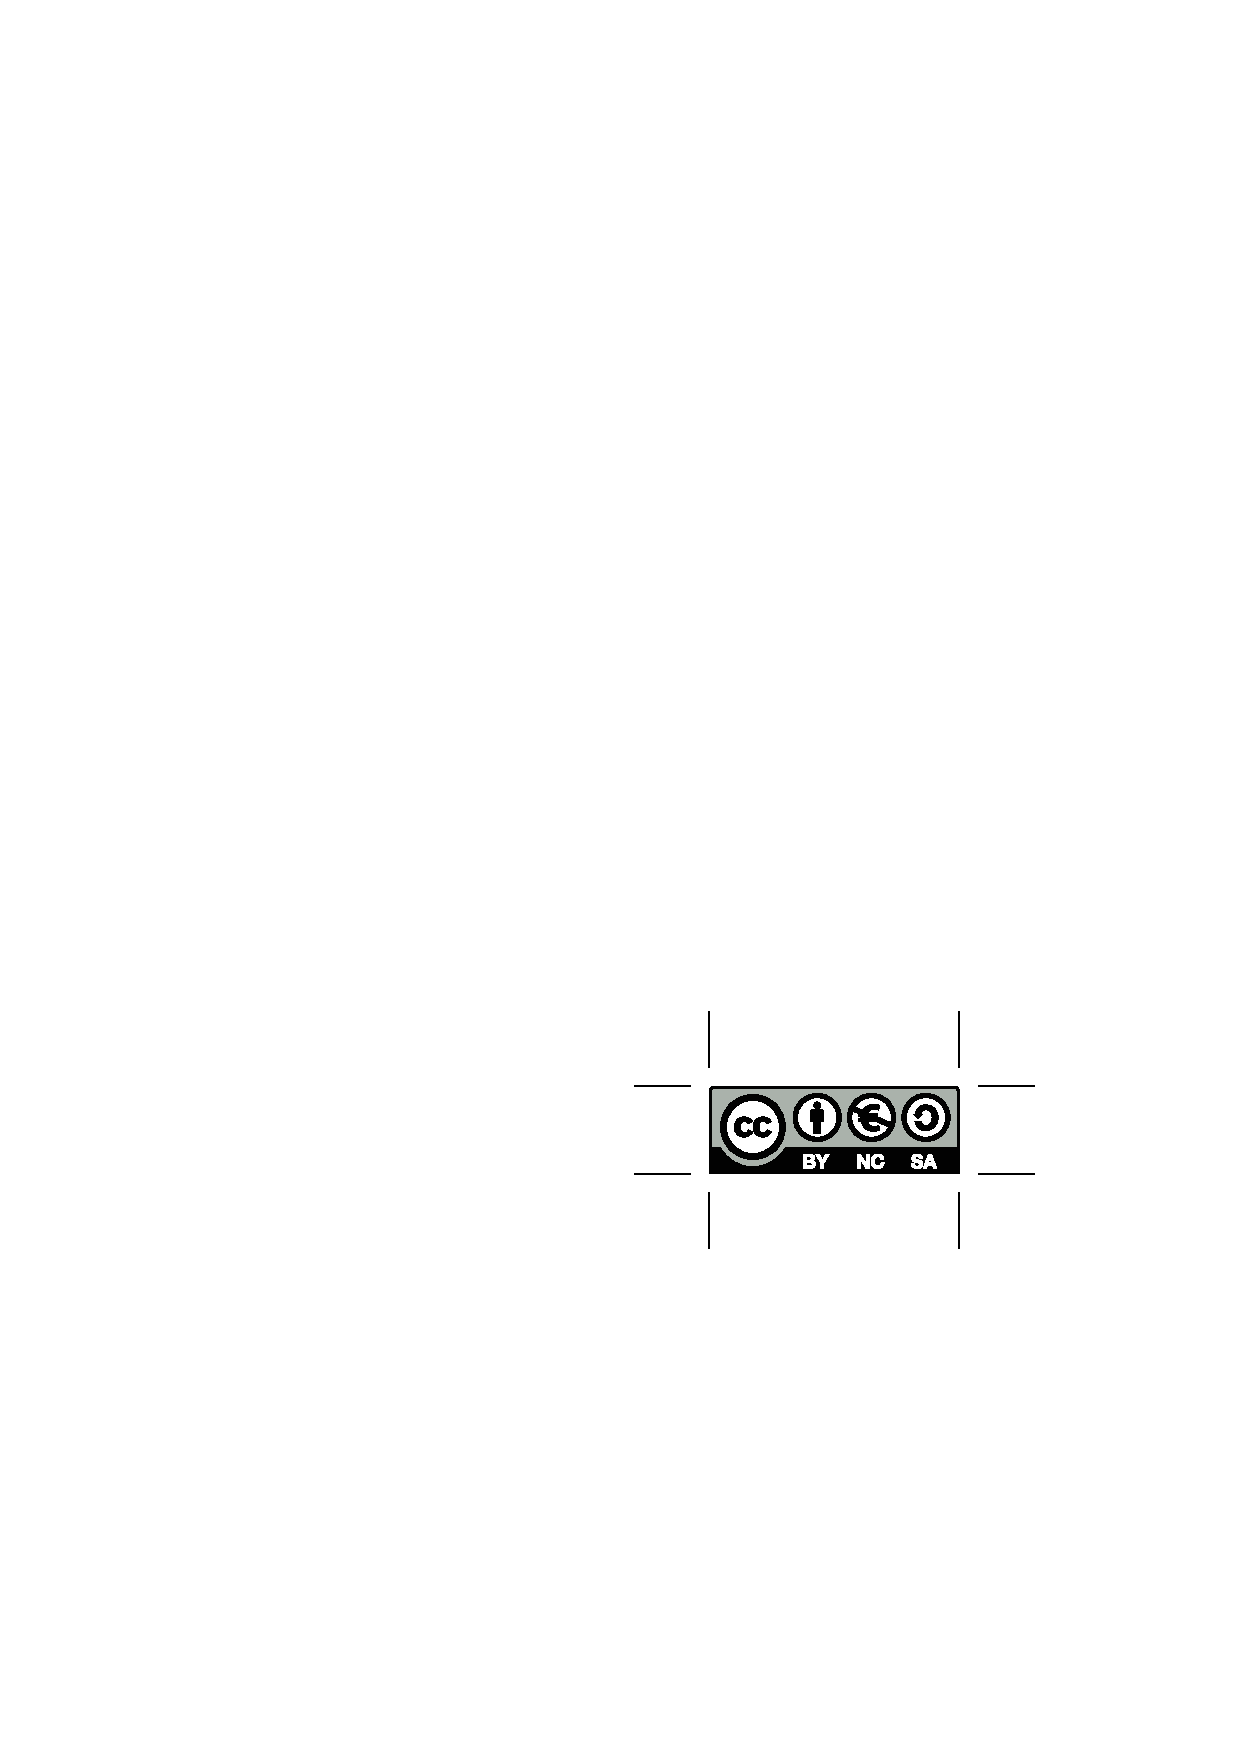
\includegraphics[width=6em]{latex/bync}
\end{wrapfigure}

Copyright \textcopyright\, 2020 \TeX nician og useR Andreas Kracht Frandsen

Alt indhold er licenseret under CC BY-NC-SA 4.0

\textit{Sat med Palatino Linotype}

\newpage

\pagenumbering{roman}

{
  \hypersetup{linkcolor=black}
  \tableofcontents
}

\newpage

{
  \hypersetup{linkcolor=black}
  \listoffigures

  \listoftables
}

\newpage

\hypertarget{forord}{%
\chapter*{Forord}\label{forord}}
\addcontentsline{toc}{chapter}{Forord}

Kreditering: \href{http://starlogs.net/\#afrandsen/master-thesis}{starlogs.net/\#afrandsen/master-thesis}.

Dokumentet er i farver, men kan printes i sort/hvid uden at skabe visuelle mangler på plots, da linjer samt punkter har hhv. forskellige linjetyper og symboler.

Farver igennem hele dokumentet er sat via pakken \emph{RColorBrewer} og dens tilhørende farvepalete \emph{Dark2}. Denne farvepalette tillader, at personer med nedsat farvesyn uden problemer kan skelne linjer, punkter osv. fra samtlige plots. Derudover er paletten printervenlig samt LCD-venlig.

Gennem hele dokumentet er der anvendt \emph{fictitious entry}, der fungerer som en \emph{copyright trap}.
\newpage

\pagenumbering{arabic}

\setcounter{secnumdepth}{3}

\part{Introduktion og litterært overblik}

\hypertarget{indledning}{%
\chapter{Indledning}\label{indledning}}

Denne afhandling har til formål at undersøge langsigtet investering i aktiver under antagelsen om periodisk rebalancering. Dette gøres ved anvendelse af den analytiske løsning, til det dynamiske porteføljeproblem, først beskrevet af \citep{JurVic2011}. Denne løsning anvendes for en institutionel/privat investor med endelig investeringshorisont, tidsvarienede investeringsmuligheder og under antagelsen om potens nytte, \emph{CRRA}, defineret over deres intertemporale budgetbegræsning gennem formue. Sættet af tidsvarierende investeringsmuligheder er konstante under hele investeringshorisonten, dette gør, at en sammenligning af investorer, med en kort og en lang investeringshorisont samt med forskellige risikotolerancer, kan udarbejdes. Investeringssættet, som spænder fra 1952 2. kvartal til 2018 4. kvartal, består af en 90-dages amerikansk \emph{T-Bill} -- som samtidig repræsenterer benchmarkaktivet -- et aktieindeks, som repræsenterer samtlige aktier handlet på \emph{NYSE}, \emph{AMEX} og \emph{NASDAQ}, den 10-årige amerikanske statsobligation samt et virksomhedsbaseret obligationsindeks. Før modellering af merafkastene på ovenstående aktiver over benchmarkaktivet, undersøges prædiktabiliteten af afkastene, ved benyttelse af relevante finansielle, rentestruktur og makroøkonomiske variable, som før har vist prædiktablitetsegenskaber i eksisterende litteratur. Selve modellen af tilstandsvariablene antages at følge en første-ordens \emph{Vector Autoregressive Process}. Analysen viser at variansen på aktier, faktoren \emph{Small Minus Big} samt det korte rentespænd \emph{Yield Spread}, generelt for alle aktivklasser udviser størst statistisk signifikans. Derudover findes der evidens for, at afkastene på de risikobærende aktiver specielt er tidsvarierende. Afkastet på aktieindekset viser sig, at være sværest prædiktabelt, mens stats- og virksomhedsobligationerne bevæger sig procyklisk med yield spread. Porteføljevalget for investoren afhænger kraftigt af disse afkastbevægelser, da han udnytter denne information til at lave periodiske reblancereringer ift. sin risikoaversion. Ved undersøgelse af både investeringshorisontlængdens effekt, risikotolerancer og effekten af korte posisitoner kan forskellen mellem en lang række af investorer effektivt måles.

\hypertarget{problemformulering}{%
\section{Problemformulering}\label{problemformulering}}

Ved analytisk behandling af det dynamiske porteføljeproblem, vil denne afhandling undersøge, hvordan porteføljeallokeringer adskiller sig: på tværs af investeringshorisonter, ved restriktioner af korte positioner i aktiver og ved forskellige tolerancer for risiko.

\begin{center}
\textit{Hvordan adskiller porteføljeallokeringen sig over investeringshorisonter, for den institutionelle og/eller private investor, under antagelsen, at der er mulighed for periodisk rebalancering?}
\end{center}

De underliggende spørgsmål, som ligger i forlængelse af det ovenstående grundlæggende spørgsmål, vil undervejs i afhandlingen ligeledes blive behandlet og undersøgt, heriblandt, hvordan risikotolerancer hos individuelle investorer påvirker allokeringen af risikobærende aktiver.

\hypertarget{afgruxe6nsning}{%
\section{Afgrænsning}\label{afgruxe6nsning}}

Denne afhandling forsøger at svare på ovenstående hovedspørgsmål ved benyttelse af empirisk data. I forlængelse af søgen efter et sådant svar, vil en teoretisk afgrænsning være nødvendig. Menneskelig kapital samt forbrug vil af den grund ikke være en del af den empiriske analyse. Dette er også ensbetydende med at budgetbegrænsningen for hver institutionelle og/eller private investor er fuldstændig fastsat ud fra deres finansielle formue.

Investorerne antages til at have deres nytte defineret via \emph{CRRA}-nytte. For at anvende \emph{CRRA}-nytte i porteføljeproblemet benyttes modellen fra \citep{JurVic2011}, som er defineret i diskrettid, med approksimative analytiske løsninger. Dette medfører bl.a. at det dynamiske porteføljeproblem i kontinuert tid bliver tilsidesat, da hovedformålet med afhandlingen er at undersøge det langsigtede porteføljevalg på diskrete tidspunkter over investorens investeringshorisont. Derudover ville en kontinuert behandling af det dynamiske porteføljeproblem ligeledes kræve en diskretisering af observationsrummet for anvendelse i et empirisk øjemed. Ved anvendelse af den teoretiske ramme foreslået af \citep{JurVic2011} antages det samtidigt, at investorens nytte kun er defineret over hans intertemporale budgetbegrænsning og over en fastlagt investeringshorisont med tidsvarierende investeringsmuligheder, som er modelleret via en VAR\((1)\)-process.

Robustheden af den empiriske analyse er begrænset, eftersom eksogen stikprøvekontrol ikke bliver udført. Undersøgelsen indebærer kvartalsvise finansielle, rentestrukturelle og makroøkonomiske data fra 1954 2. kvartal til 2018 4. kvartal, dette betyder også, at de endelige resultater kan være signifikant forskellige fra analytiske metoder, som indebærer månedlige eller årlige data. Analysen vil ikke indebære transaktionsomkostninger, hvilket før har vist at have væsentlige betydninger for de endelige porteføljevalg, specielt for den myopiske investor, \citep{BalLyn1999}. Afhandlingen vil ikke indeholde en performance-mæssig evaluering -- på baggrund af porteføljevalgene -- ift. investeringsomkostninger. Derudover begrænses analysen af, at den ignorerer problemerne ved at investere til pension og dermed undgår kompleksiteterne ved levetid, aldring og tidsafhængige ændringer i karakteristika af markedsdeltagere og demografiske forhold, som indgår i det såkaldte \emph{life-cycle} problem.

Til forskel for ovenstående begrænsninger vil denne afhandling fokusere på, hvordan porteføljeallokeringer adskiller sig: på tværs af investeringshorisonter og ved forskellige tolerancer for risiko. Givet at investoren står overfor endelige investeringshorisonter og tidsvarierende investeringsmuligheder.
En analyse af kortsalgsrestriktion på porteføljeproblemet er ligeledes medtaget i afhandlingen, men omkostningerne ved lån/gearing af den optimale portefølje er udeladt.

Ved at begrænse analysen for porteføljevalget, kan vi evaluere porteføljeallokeringerne baseret på de samme antagelser, hvor kun den intertemporale budgetbegrænsning og/eller risikoaversionen adskiller hver enkelt investor.

\hypertarget{eksisterende-litteratur}{%
\section{Eksisterende litteratur}\label{eksisterende-litteratur}}

En langsigtet porteføljestrategi forsøger at optimere bytteforholdet mellem risiko og afkast. En sådan strategi er i sagens natur optimal på lang sigt og ikke nødvendigvis på kort sigt. Den moderne teori bag dette bytteforhold, for den langsigtede investor, blev først beskrevet af Nobelpris modtageren Harry Markowitz, \citep{Markowitz1952}. Hans arbejde tager udgangspunkt i en investor på tidspunkt \(t\), som kun bekymrer sig om fordelingen af sin formue på et givet fremtidigt tidspunkt \(t+K\), hvor \(K\) er investeringshorisonten. Dette problem bliver undertiden beskrevet som det statiske portefølje problem. \citep{Markowitz1952} understreger vigtigheden af diversifikation af risiko, men den bærende antagelse om en køb og hold investor, findes generelt særdeles urealistisk. Investorer vælger ofte porteføljestrategier, som kræver rebalancering før eller siden, og er på den måde dynamiske i deres optimeringsstrategi.

Mere generelt vil investorer altså rebalancere deres portefølje mellem tidspunkt \(t\) og \(t+K\), på en måde, som forholder sig til skiftende finansielle, rentestrukturelle og makroøkonomiske forhold over tid. Investoren vil altså i dette tilfælde vælge en dynamisk porteføljestrategi, som specificerer, hvordan allokeringen af en eller flere aktiver skal ændres i respons til de tidsafhængige bagvedliggende variable.

Dynamisk programmering er før blevet brugt i litteraturen til at formulere en løsning, \citep{Mossin1968}, \citep{Samuelson1969} og \citep{Merton1969, Merton1971, Merton1973}. Udover de specialtilfælde, hvor den langsigtede porteføljestrategi består af en række optimale kortsigtede strategier, er ingen generel løsning på lukket form udledt, \citep{JurVic2011}. \citep{Samuelson1969} introducerer også en model, som medtager forbrugsfunktionen. \citep{Merton1969} beskriver den dynamiske allokering i kontinuert tid til forskel fra de tidligere diskrettidsmodeller af bl.a. \citep{Samuelson1969}. Derudover beskriver \citep{Merton1969}, hvordan en flerdimensional stokastisk model -- hvor de underliggende variable er modelleret via en Wiener process -- giver en rigere og mere alsidig model.

På baggrund af det svære løsningsproblem, var der over længere tid en faldende interesse for emnet, men nylig videnskabelig litteratur af finansielle økonomer har atter kastet lys på emnet. Disse foreslår alternative løsningsmetoder for det langsigtede porteføljeproblem med rebalancering, og har igen fundet eksakte analytiske løsninger for yderligere specialtilfælde, i kontinuert tid, end de tidligere beskrevne. Ved antagelse af en konstant risikofri rente og modellering af merafkastet gennem en Ornstein-Uhlenbeck process finder \citep{BrenXia2002}, \citep{CampVic1999}, \citep{KimOm1996} og \citep{Wachter2002} løsninger på lukket form for en lang række nyttefunktioner, heriblandt potens nytte over forbrug, potens nytte over terminal formue og for Epstein-Zin nytte med intertemporal substitutionselasticitet lig én, \citep{CampVic2003}.

Derudover er numeriske metoder blevet foreslået af bl.a. \citep{BalLyn1999}, \citep{Lyn2001}, \citep{Bar2000}, \citep{BrenSchLag1997, BrenSchLag1999}, hvor de anvendte modeller enten har diskretiseret observationsrummet eller fundet numeriske løsninger til den partielle differentialligning hørende til det dynamiske problem. Disse -- til tider avancerede -- numeriske metoder har dog vist sig at være svært anvendelige. I praksis har det været komplekst at implementere selv for få variable.

Ovenstående modeller tillader ikke den risikofrie rente og merafkastet af aktiver at ændre sig over tid på samme tid, og mangler dermed det tidsvarierende perspektiv af alle aktiver. En ny metode præsenteret af \citep{CampVic1999, CampVic2001, CampVic2003}, giver approksimative analytiske metoder i et ikke-tilfældigt nabolag af specialtilfælde, hvor løsninger på lukket form er mulige. Her tager de udgangspunkt i en investor, som opnår nytte af forbrug i stedet for formue. \citep{CampVicCha2003} benytter samme metode til et problem involverende flere risikofyldte aktivklasser, hvor de samtidig tillader tidsvarierende investeringsmuligheder.

Mit arbejde vil være en validering af \citep{JurVic2011} ved anvendelse af deres teori samt analytiske løsninger til det dynamiske porteføljeproblem for en institutionel/privat investor med et opdateret datagrundlag. Jeg bidrager til det dynamiske porteføljeproblem ved en længere statistisk analyse af potentielle variable, som kan benyttes til det prædiktive afspekt af flere aktivers afkast.

\hypertarget{opbygning-samt-tekniske-specifikationer}{%
\section{Opbygning samt tekniske specifikationer}\label{opbygning-samt-tekniske-specifikationer}}

Opbygningen af denne afhandling tager udgangspunkt i dele. Første del fungerede som en introduktion til litteraturen og afhandlingens formål. I Del 2 af afhandlingen fastlægges det teoretiske fundament. Kapitel 2 giver et overblik over den underliggende porteføljeteori for en institutionel investor. Kapitel 3 præsenterer aktivklasserne og deres relationer med potentielle prædiktive variable samt opbygningen af afkast gennem nutidsværdi. Derudover præsenterer kapitlet en lang række potentielle prædiktionsvariable. Kapitel 4 bygger videre fra teorien i Kapitel 3, og fastlægger den analytiske løsning til det dynamiske porteføljeproblem og medtager dermed rebalanceringsperspektivet. Kapitel 5 opbygger den dynamiske ramme i form af VAR-processen for vores investeringssæt. Del 3 består af den empiriske analyse, hvor teorien fra Del 2 benyttes på virkeligt data. Kapitel 6 beskriver data samt kilder. Kapitel 7 består af univariate- og multiple regressioner, som benyttes til undersøgelse af variablene med bedste prædiktabilitetsegenskaber til den endelige VAR-model. Kapitel 8 har til formål at præsentere et overblik over den endelige VAR-model. Kapitel 9 undersøger problemerne ved estimation. Kapitel 10 foretager analysen af samtlige porteføljeallokeringer. Kapitel 11 indeholder en diskussion og reflektion over fundende i Kapitel 10. Til slut afslutter Kapitel 12 afhandlingen med en konklusion.

Databehandling samt modelestimation er beregnet og kodet via statistikprogrammet \textbf{R} 3.6.0 \emph{``Planting of a Tree''}. \textbf{R}-pakker med teoretisk dokumentation er anvendt ved estimation af VAR-processen samt for de univariate- og multiple regressioner, for yderligere information henvises til dokumentationen i litteraturlisten. Denne version af afhandlingen blev bygget med:

\begin{verbatim}
## - Session info ---------------------------------------------------------------
##  setting  value                       
##  version  R version 3.6.0 (2019-04-26)
##  os       Windows 10 x64              
##  system   x86_64, mingw32             
##  ui       RTerm                       
##  language (EN)                        
##  collate  English_United States.1252  
##  ctype    English_United States.1252  
##  tz       Europe/Paris                
##  date     2020-06-01                  
## 
## - Packages -------------------------------------------------------------------
##  package       * version  date       lib source           
##  assertthat      0.2.1    2019-03-21 [1] CRAN (R 3.6.0)   
##  backports       1.1.6    2020-04-05 [1] CRAN (R 3.6.3)   
##  bookdown        0.18     2020-03-05 [1] CRAN (R 3.6.3)   
##  broom           0.5.6    2020-04-20 [1] CRAN (R 3.6.3)   
##  callr           3.4.3    2020-03-28 [1] CRAN (R 3.6.3)   
##  cellranger      1.1.0    2016-07-27 [1] CRAN (R 3.6.0)   
##  cli             2.0.2    2020-02-28 [1] CRAN (R 3.6.3)   
##  colorspace      1.4-1    2019-03-18 [1] CRAN (R 3.6.0)   
##  crayon          1.3.4    2017-09-16 [1] CRAN (R 3.6.0)   
##  curl            4.3      2019-12-02 [1] CRAN (R 3.6.3)   
##  DBI             1.1.0    2019-12-15 [1] CRAN (R 3.6.3)   
##  dbplyr          1.4.3    2020-04-19 [1] CRAN (R 3.6.3)   
##  desc            1.2.0    2018-05-01 [1] CRAN (R 3.6.0)   
##  devtools        2.3.0    2020-04-10 [1] CRAN (R 3.6.3)   
##  digest          0.6.25   2020-02-23 [1] CRAN (R 3.6.3)   
##  dplyr         * 0.8.5    2020-03-07 [1] CRAN (R 3.6.3)   
##  ellipsis        0.3.0    2019-09-20 [1] CRAN (R 3.6.3)   
##  evaluate        0.14     2019-05-28 [1] CRAN (R 3.6.0)   
##  fansi           0.4.1    2020-01-08 [1] CRAN (R 3.6.3)   
##  forcats       * 0.5.0    2020-03-01 [1] CRAN (R 3.6.3)   
##  fs              1.4.1    2020-04-04 [1] CRAN (R 3.6.3)   
##  generics        0.0.2    2018-11-29 [1] CRAN (R 3.6.0)   
##  ggfortify     * 0.4.9    2020-03-11 [1] CRAN (R 3.6.3)   
##  ggplot2       * 3.3.0    2020-03-05 [1] CRAN (R 3.6.3)   
##  glue            1.4.0    2020-04-03 [1] CRAN (R 3.6.3)   
##  gridExtra       2.3      2017-09-09 [1] CRAN (R 3.6.3)   
##  gtable          0.3.0    2019-03-25 [1] CRAN (R 3.6.0)   
##  haven           2.2.0    2019-11-08 [1] CRAN (R 3.6.3)   
##  hms             0.5.3    2020-01-08 [1] CRAN (R 3.6.3)   
##  htmltools       0.4.0    2019-10-04 [1] CRAN (R 3.6.3)   
##  httr            1.4.1    2019-08-05 [1] CRAN (R 3.6.1)   
##  IntroCompFinR * 1.0      2015-10-30 [1] R-Forge (R 3.6.0)
##  jsonlite        1.6.1    2020-02-02 [1] CRAN (R 3.6.3)   
##  knitr           1.28     2020-02-06 [1] CRAN (R 3.6.3)   
##  lattice         0.20-38  2018-11-04 [2] CRAN (R 3.6.0)   
##  lifecycle       0.2.0    2020-03-06 [1] CRAN (R 3.6.3)   
##  lmtest        * 0.9-37   2019-04-30 [1] CRAN (R 3.6.1)   
##  lubridate       1.7.8    2020-04-06 [1] CRAN (R 3.6.3)   
##  magrittr        1.5      2014-11-22 [1] CRAN (R 3.6.0)   
##  MASS          * 7.3-51.4 2019-03-31 [2] CRAN (R 3.6.0)   
##  memoise         1.1.0    2017-04-21 [1] CRAN (R 3.6.0)   
##  modelr          0.1.6    2020-02-22 [1] CRAN (R 3.6.3)   
##  moments       * 0.14     2015-01-05 [1] CRAN (R 3.6.0)   
##  munsell         0.5.0    2018-06-12 [1] CRAN (R 3.6.0)   
##  nlme            3.1-147  2020-04-13 [1] CRAN (R 3.6.3)   
##  pillar          1.4.3    2019-12-20 [1] CRAN (R 3.6.3)   
##  pkgbuild        1.0.6    2019-10-09 [1] CRAN (R 3.6.3)   
##  pkgconfig       2.0.3    2019-09-22 [1] CRAN (R 3.6.3)   
##  pkgload         1.0.2    2018-10-29 [1] CRAN (R 3.6.0)   
##  prettyunits     1.1.1    2020-01-24 [1] CRAN (R 3.6.3)   
##  processx        3.4.2    2020-02-09 [1] CRAN (R 3.6.3)   
##  ps              1.3.2    2020-02-13 [1] CRAN (R 3.6.3)   
##  purrr         * 0.3.4    2020-04-17 [1] CRAN (R 3.6.3)   
##  quantmod      * 0.4.17   2020-03-31 [1] CRAN (R 3.6.3)   
##  R6              2.4.1    2019-11-12 [1] CRAN (R 3.6.3)   
##  RColorBrewer  * 1.1-2    2014-12-07 [1] CRAN (R 3.6.0)   
##  Rcpp            1.0.4.6  2020-04-09 [1] CRAN (R 3.6.3)   
##  readr         * 1.3.1    2018-12-21 [1] CRAN (R 3.6.0)   
##  readxl          1.3.1    2019-03-13 [1] CRAN (R 3.6.0)   
##  remotes         2.1.1    2020-02-15 [1] CRAN (R 3.6.3)   
##  reprex          0.3.0    2019-05-16 [1] CRAN (R 3.6.0)   
##  rlang           0.4.5    2020-03-01 [1] CRAN (R 3.6.3)   
##  rmarkdown       2.1      2020-01-20 [1] CRAN (R 3.6.3)   
##  rprojroot       1.3-2    2018-01-03 [1] CRAN (R 3.6.0)   
##  rstudioapi      0.11     2020-02-07 [1] CRAN (R 3.6.3)   
##  rvest           0.3.5    2019-11-08 [1] CRAN (R 3.6.3)   
##  sandwich      * 2.5-1    2019-04-06 [1] CRAN (R 3.6.1)   
##  scales          1.1.0    2019-11-18 [1] CRAN (R 3.6.3)   
##  sessioninfo     1.1.1    2018-11-05 [1] CRAN (R 3.6.0)   
##  stringi         1.4.6    2020-02-17 [1] CRAN (R 3.6.2)   
##  stringr       * 1.4.0    2019-02-10 [1] CRAN (R 3.6.0)   
##  strucchange   * 1.5-2    2019-10-12 [1] CRAN (R 3.6.1)   
##  testthat        2.3.2    2020-03-02 [1] CRAN (R 3.6.3)   
##  tibble        * 3.0.1    2020-04-20 [1] CRAN (R 3.6.3)   
##  tidyr         * 1.0.2    2020-01-24 [1] CRAN (R 3.6.3)   
##  tidyselect      1.0.0    2020-01-27 [1] CRAN (R 3.6.3)   
##  tidyverse     * 1.3.0    2019-11-21 [1] CRAN (R 3.6.3)   
##  TTR           * 0.23-6   2019-12-15 [1] CRAN (R 3.6.3)   
##  urca          * 1.3-0    2016-09-06 [1] CRAN (R 3.6.1)   
##  usethis         1.6.0    2020-04-09 [1] CRAN (R 3.6.3)   
##  VAR.etp       * 0.7      2014-12-02 [1] CRAN (R 3.6.0)   
##  vars          * 1.5-3    2018-08-06 [1] CRAN (R 3.6.1)   
##  vctrs           0.2.4    2020-03-10 [1] CRAN (R 3.6.3)   
##  withr           2.2.0    2020-04-20 [1] CRAN (R 3.6.3)   
##  xfun            0.13     2020-04-13 [1] CRAN (R 3.6.3)   
##  xml2            1.3.2    2020-04-23 [1] CRAN (R 3.6.0)   
##  xts           * 0.12-0   2020-01-19 [1] CRAN (R 3.6.3)   
##  yaml            2.2.1    2020-02-01 [1] CRAN (R 3.6.2)   
##  zoo           * 1.8-7    2020-01-10 [1] CRAN (R 3.6.3)   
## 
## [1] C:/Users/AKF/Documents/R/win-library/3.6
## [2] C:/Program Files/R/R-3.6.0/library
\end{verbatim}

Litterær programmering er blevet anvendt til at skrive/programmere denne afhandling i tekstformattet \emph{.Rmd}, for herefter at blive processeret af \emph{knitr} til et \emph{.md} format, denne fil føres videre til \emph{pandoc}, som har til ansvar at danne den færdige fil. Denne to-trins operation tillader at danne afhandlingen i en lang række filformater. I den forbindelse er versionsstyring samtidig blevet anvendt gennem \emph{GitHub}. Af den grund er den fulde kildekode tilgængelig via \href{https://github.com/afrandsen/master-thesis}{github.com/afrandsen/master-thesis}.

\newpage

\part{Den teoretiske ramme}

\hypertarget{unteo}{%
\chapter{Underliggende teori}\label{unteo}}

I dette kapitel introduceres den underliggende teori til det dynamiske porteføljeproblem: det statiske porteføljeproblem. Derudover defineres en række nyttefunktioner, som alle er defineret over terminalformue. Sektion \ref{myoinv} starter med en gennemgang af porteføljeproblemet for den myopiske investor, som først blev introduceret af \citep{Markowitz1952}. Dernæst fungerer Sektion \ref{preforris} som en introduktion til risikoaversion. Sektion \ref{nytdefover} belyser en række nyttefunktioner, som alle kan fungere i porteføljemodellering. Fordelingsmæssige resultater vedr. afkast tages hånd om i Sektion \ref{fordafafk}. Slutteligt opsummerer Sektion \ref{opsunteo} kapitlets fund.

\hypertarget{myoinv}{%
\section{Den myopiske investor}\label{myoinv}}

Den myopiske investor vælger -- som navnet ligger op til -- sin portefølje under et én-periodes perspektiv, og foretager dermed et statisk bindende valg. Investoren forsøger at maksimere sin terminal formue, ved samtidig at forholde sig til sin risikoaversion. Dette forårsager, at alle efterfølgende perioder bliver ignoreret af investoren. Ergo skal han løse det statiske portefølje problem fra tidspunkt \(t\) til tidspunkt \(t+1\). I denne ene periode antages investeringsmulighederne at være: et risikobærende aktiv samt et risikofrit aktiv. Afkastene over den førstkommende periode for disse aktivklasser vil blive noteret som hhv. \(R_{t+1}\) med betinget middelværdi \(\mathbb{E}_t\left[R_{t+1}\right]\)\footnote{Her benyttes den gængse notation \(\mathbb{E}\left[R_{t+1}\mid \mathcal{F}_t\right]=\mathbb{E}_t\left[R_{t+1}\right]\) for filteret \(\mathcal{F}_t\).} samt betinget varians \(\mathbb{V}_t\left[R_{t+1}\right]=\sigma_t^2\) og \(R_{0,t+1}\).

Det antages at investorens formue er fuldt allokeret når en del \(\alpha_t\) bliver placeret i det risikobærende aktiv og \((1-\alpha_t)\) i det risikofrie aktiv. Hermed bliver hans porteføljeafkast givet ved
\begin{equation}
R_{p,t+1}=\alpha_t R_{t+1}+\left(1-\alpha_t\right)R_{0,t+1}.\label{eq:Portafk}
\end{equation}

Den betingede middelværdi af porteføljeafkastet bliver dermed
\begin{align}
\mathbb{E}_t\left[R_{p,t+1}\right]&=\alpha_t\mathbb{E}_t\left[R_{t+1}\right]+(1-\alpha_t)R_{0,t+1} \notag\\ 
&=R_{0,t+1}+ \alpha_t\left(R_{t+1} - R_{0,t+1}\right),\label{eq:Forvport}
\end{align}

og endeligt den betingede varians af porteføljeafkastet
\begin{equation}
\mathbb{V}_t\left[R_{p,t+1}\right]=\alpha_t^2\sigma_t^2.\label{eq:Varport}
\end{equation}

Den simplificerende antagelse i \citep{Markowitz1952} er, at investorer kun forholder sig til de første to momenter, hvis vi modellerer denne afvejning lineært, opnår vi følgende maksimeringsproblem
\begin{equation}
\max_{\alpha_t} \mathbb{E}_t\left[R_{p,t+1}\right] -\frac{k}{2} \mathbb{V}_t\left[R_{p,t+1}\right],\label{eq:Statmaks}
\end{equation}

hvor \(k\) er en skalering, som repræsenterer investorens risikoaversion. Ved at modellere ovenstående relation som lineær og kun afhængig af de første to momenter restringeres investoren til at foretrække et højt afkast, lav volatilitet og ignorerer alle højere momenter, såsom skævhed og kurtosis. Ved indsættelse af Ligning \eqref{eq:Portafk} i Maksimeringsproblemet \eqref{eq:Statmaks} og dernæst differentiation opnåes førsteordensbetingelsen, se Appendiks \ref{udlmyo}, løsningen til optimalitetsproblemet bliver
\begin{equation}
\alpha_t = \frac{\mathbb{E}_t\left[R_{t+1}\right]-R_{0,t+1}}{k\sigma_t^2}.\label{eq:Løsning}
\end{equation}

Porteføljeanalyse benytter ofte nøgletallet \emph{Sharpe Ratio}, også kendt som \emph{Market Price of Risk} i stokastisk finansiering, \citep{Bjork2009}. I porteføljeteori er det kendt som et performance-mål, som fortæller investoren om merafkastet i sin portefølje relativt til den risiko han har påtaget sig, altså
\[S_t=\frac{\mathbb{E}_t\left[R_{t+1}\right]-R_{0,t+1}}{\sigma_t}.\]

Dette tillader, at vi kan omskrive Ligning \eqref{eq:Løsning} til
\[\alpha_t=\frac{S_t}{k\sigma_t}.\]

Forholdet mellem middelværdien og variansen er \(\tfrac{1}{k}\), eftersom vi kan udlede, at merafkastet på porteføljen er \(\tfrac{S_t^2}{k}\) og variansen er \(\tfrac{S_t^2}{k^2}\). \emph{Sharpe Ratio}'en på porteføljen er \(S_t\), og alle tænkelige porteføljer (afhængig af \(k\)) vil have samme \emph{Sharpe Ratio}, fordi de er eksponeret til det risikobærende aktiv, men i stadig større eller mindre grad.

Altså er vægtningen i det risikobærende aktiv et forhold mellem: det forventede risikobærende merafkast over det risikofrie aktiv samt en skalering af det risikobærende aktivs varians. Vi kan uden problemer opskrive ovenstående løsning til tilfældet, hvor investoren står overfor \(n>1\) risikobærende aktiver. \(\bm{R}_{t+1}\) repræsenterer en \(n\times 1\) vektor af afkast for risikobærende aktiver, fra \(t\) til \(t+1\). Den betingede middelværdi bliver \(\mathbb{E}_t\left[\bm{R}_{t+1}\right]\) og den betingede kovariansmatrix noteres som \(\mathbb{V}_t\left[\bm{R}_{t+1}\right]=\bm{\Sigma}_t\). Herudover er \(\bm{\alpha}_t\) nu en \(n\times 1\) vektor af vægte i de risikobærende aktiver.

Den betingede middelværdi af porteføljeafkastet bliver dermed nu
\begin{equation}
\mathbb{E}_t\left[R_{p,t+1}\right]=R_{0,t+1}+\bm{\alpha}_t'(\mathbb{E}_t\left[\bm{R}_{t+1}\right]- R_{0,t+1}\bm{\ell}),
\end{equation}

den betingede varians af porteføljeafkastet bliver
\begin{equation}
\mathbb{V}_t\left[R_{p,t+1}\right]=\bm{\alpha}_t'\bm{\Sigma}_t\bm{\alpha}_t.
\end{equation}

Nu kan maksimeringsproblemet opskrives
\begin{equation}
\max_{\alpha_t} \bm{\alpha}_t'(\mathbb{E}_t\left[\bm{R}_{t+1})- R_{0,t+1}\bm{\ell}\right] - \frac{k}{2}\bm{\alpha}_t'\bm{\Sigma}_t\bm{\alpha}_t, \label{eq:MultStatmaks}
\end{equation}

Den optimale porteføljestrategi, givet som løsningen til Maksimeringsproblemet \eqref{eq:MultStatmaks} findes til at være
\begin{equation}
\bm{\alpha}_t=\frac{1}{k}\bm{\Sigma}_t^{-1}(\mathbb{E}_t\left[\bm{R}_{t+1}\right]-R_{0,t+1}\bm{\ell}).\label{eq:Multalpha}
\end{equation}

Løsningen er en generalisering af Ligning \eqref{eq:Løsning}. Derudover er det værd at bemærke, at løsningen er karakteriseret af \textit{The Mutual Fund Seperation Theorem}, \citep{Tobin1958}, som var en af mange videnskabelige bidrag James Tobin fik sin Nobelpris for i 1981, \citep{Nobel2020}. Essencen af Sætningen er, at alle investorer vil holde den eksakt samme portefølje af risikobærende aktiver samt en del i det risikofrie aktiv. Det eneste som adskiller investorer fra hinanden, er deres relative fordeling af total formue i den optimale risikobærende portefølje, som er fastsat ud fra deres egne risikopræferencer. Figur \ref{fig:AfkVol} viser de optimale porteføljestrategier i et afkast-volatilitets spektrum.

\begin{figure}[H]
\centering
\begin{tikzpicture}[scale=1]
\begin{axis}[
  xticklabel={$\pgfmathprintnumber{\tick}\,\%$},
  yticklabel={$\pgfmathprintnumber{\tick}\,\%$},
  height=7cm, width=12cm,
  axis x line=bottom, axis y line=left,
  xlabel = Standardafvigelse, ylabel = Forventet afkast,
  ymin=0, ymax=25, xmin=0, xmax=60,
  extra x ticks={65}, extra x tick labels={$\sigma$},
  extra x tick style={major tick length=0mm, grid=none},
  extra y ticks={27}, extra y tick labels={$\mu$},
  extra y tick style={major tick length=0mm, grid=none},
  enlargelimits=true,
  scatter/classes={
    a={mark=o,draw=black, mark size = 3pt},
    b={mark=*, mark size = 3pt,draw=red, fill = red},
    c={mark=*, mark size = 3pt,draw=black, fill = black}
  }
]

\addplot[scatter,only marks, scatter src=explicit symbolic]
  coordinates {
    (30, 11)     [c]
    (19, 5)      [c]
    (40, 15)     [c]
    (16, 10)     [b]
  };
\node at (axis cs:19, 5) [anchor=north west] {Aktiv 1};
\node at (axis cs:30,11) [anchor=north west] {Aktiv 2};
\node at (axis cs:40,15) [anchor=north west] {Aktiv 3};
\addplot[red, very thick,  domain=-1:2.5, samples=200, variable=\t](
   {(20^2*t^2 + 12^2*(1-t)^2)^(0.5) }, %{(t^2 * 20^2 + (1-t)^2 * 12)},
   {11 * t + (1-t) * 5}
 );
\node[color=red] at (axis cs:30, 0) [anchor=south west] {\textbf{Den efficiente rand}};
\addplot[black, very thick, domain=-10:50, samples=100, variable=\x](
  ({x}, {4 + 0.37 * x});
\node[rotate = 25, color=black] at (axis cs:30, 15) [anchor=south west] {\textbf{CML}};
\node[pin={[pin edge={thick}, text width=3cm, pin distance=2cm]90:{{\centering Tangensporteføljen}}}] at (axis cs:16, 10.5) {};
\end{axis}
\end{tikzpicture}
\caption{Afkast-volatilitets spektrummet.}
\label{fig:AfkVol}
\end{figure}

Altså vil investorer vælge en portefølje på den efficiente rand, som opnår en efficient porteføljevægtning langs \emph{Capital Market Line}. Derudover skal det nævnes, at det kun er den øvre halvdel af den efficiente rand, som reelt set er efficient. Dette kommer sig af at porteføljer på den nederste del har en identisk påhæftet volatilitet, men med et lavere forventet afkast end den symmetrisk modsatte portefølje.

Selvom Markowitz' model er en hjørnesten inden for moderne porteføljeteori, er der flere mangler i den opsatte teoretiske ramme. Først og fremmest medfører Markowitz' antagelse om en lineær afvejning mellem kovarianser og afkast implicit antagelsen, at investorenes nyttefunktioner kan approksimeres af en anden ordens Taylor udvidelse over en bredt sprektrum af afkast. Derudover findes ingen beskrivelse for, hvordan parameteren \(k\) er koblet til investorens nyttefunktion. Disse mangler kan blive afhjulpet ved samtidig brug af specifikke nyttefunktioner og afkastfordelinger, som opfylder Taylor udvidelsen. Dette medfører at middelværdi-varians analysen kan benyttes for tre forskellige opsætninger, som bliver præsenteret i Sektion \ref{typnyt}, \citep{CampVic2003}.

\hypertarget{preforris}{%
\section{Præferencer for risiko}\label{preforris}}

For et fast formueniveau \(w\in \mathbb{R}_+\) betragter vi en stokastisk variabel \(X\), hvor \(\mathbb{E}(X)=0\). Derfor kan også \(w+X\) betragtes som en stokastisk variabel, der repræsenterer en fremtidig formueplan med realiseret formue \(w+\mathbb{E}(X)\), hvis \(X\) bliver realiseret. Derfor kaldes \(X\) undertiden også et fair spil, derudover haves at \(\mathbb{E}(w+X)=w\).

En (strengt) risikoavers investor vil for alle \(w\in \mathbb{R}_+\) og alle \(X\) (strengt) foretrække den sikre formue \(w\) fremfor \(w+X\). Ergo vil investoren altid afslå ethvert fair spil. Omvendt vil en (strengt) risikoelskende investor foretrække spillet og dermed \(w+X\) fremfor \(w\). Endeligt findes risikoneutrale investorer, som er indifferent mellem den sikre formue \(w\) og formuen \(w+X\). I realiteten er investorer ingen af delene, f.eks. vil nogle afslå fair spil i et ikke-tilfældigt nabolag rundt om værdien af \(w\). Dette betegnes undertiden som at være lokalt risikoavers, lokalt risikoelskende og lokalt risikoneutral.

Generelt anses investorer (og andre individer for den sags skyld) at være risikoaverse, derfor vil fokus være på denne risikopræference.

\hypertarget{nytdefover}{%
\section{Nytte defineret over formue}\label{nytdefover}}

I Sektion \ref{myoinv}, blev en af de bærende antagelser i \citep{Markowitz1952} introduceret: at investorer kun forholder sig til middelværdien og variansen af porteføljeafkast, og ikke højere momenter. Det kan tilsvarende antages, at investorer definerer deres nytte via formue på terminaltidspunktet. Dette tillader at redefinere Maksimeringsproblemet \eqref{eq:Statmaks} til nedenstående
\begin{align}
&\max\mathbb {E}_t(U(W_{t+1})) \label{eq:Nyttemaks}\\
&\text{ubb.}\,\,W_{t+1}=(1+R_{p,t+1})W_t.\notag
\end{align}

Hvor \(U(W_{t+1})\in\mathbb{R}_+\) er en konkav nyttefunktion. Investoren vil givet nyttefunktionens konkave krumning være risikoavers. Netop dette aspekt gør, at vi kan inkorporere risikoaversion, når investorens porteføljevalg skal foretages. For at fastlægge denne investorspecifikke risikoaversion benyttes derfor skalerede krumningsmål. Disse fundamentale risikoaversionsmål er kendt som \emph{Arrow-Pratt Målene for Risikoaversion}, \citep{Arrow1965} og \citep{Pratt1964}. Når nytte skal belyses, kan risikoaversion mht. den fremtidige formue \(W_{t+1}\) benyttes. Graden af krumningen på nyttefunktion giver information om investorens risikopræferencer introduceret ovenfor. Det antages at investorens nyttefunktion er strengt voksende i terminal formue -- altså er investoren grådig og foretrækker høj formue frem for en lav formue -- men i en faldende rate. Nyttefunktion vil altså have følgende karakteristika
\[U'(W)>0\quad\text{og}\quad U''(W)<0.\]

Hvor \(U'(W)\) og \(U''(W)\) er den hhv. første- og anden afledte mht. formuen \(W\). Når denne risikoaversion skal kvantificeres, skal det sikres, at målet er invariant overfor strengt positive affine transformationer. Dette er bl.a. opfyldt ved brug af \emph{Coefficient of Absolut Risk Aversion}, \citep{Arrow1965} og \citep{Pratt1964}. \emph{ARA} er defineret som den negative anden afledte af nyttefunktionen mht. formue, skaleret med den første afledte
\[\text{ARA}(W)=-\frac{U''(W)}{U'(W)}.\]

Selvom den anden afledte af nyttefunktionen er et mål for krumningen af nyttefunktionen, er det nødvendigt at skalere for at eliminere afhængigheden af abitrære størrelser, som relaterer sig til målbarheden af nytte. \emph{ARA} måler investorens absolutte dollar værdi, som han er villig til at købe, for at undgå et tab på samme absolutte størrelse. Hvis \emph{ARA} er faldende medfører det at desto mere formue en investor har, desto mere risikosøgende bliver han, altså haves at \(\text{ARA}(W)<0\), og så fremdeles. Almindeligt menes det, at \emph{ARA} burde falde, eller i det mindste ikke stige, med formue. Et relateret mål er \emph{Coefficient of Relative Risk Aversion}, \emph{RRA}, som er samtidig tager højde for investorens formue
\[\text{RRA}(W)=-\frac{WU''(W)}{U'(W)}.\]

Her måles marginal nytten og dermed investorens risikoaversion over en procentdel af formuen. Samme inferens som for \emph{ARA} kan blive udtænkt for \emph{RRA}. \emph{RRA} måler den del af formuen, som investoren vil betale for at undgå et spil på en given størrelse relativt til formuen.

De tilsvarende reciprokke af ovenstående mål kaldes hhv. \emph{Coefficeint of Absolute Risk Tolerance} samt \emph{Coefficeint of Relative Risk Tolerance}.

\begin{figure}[H]
\centering
\begin{tikzpicture}[scale=1]
\begin{axis}[
  height=7cm, width=12cm,
  axis x line=bottom, axis y line=left,
  xlabel = Formue, ylabel = Nytte,
  ymin=0, ymax=25, xmin=0, xmax=60,
  xtick={5, 15, 30}, xticklabels={$W_{t}-G$, $W_t$, $W_t+G$},
  ytick={9.7, 16.3, 20.5}, yticklabels={$U(W_{t}-G)$, $U(W_{t})$, $U(W_{t}+G)$},
    extra x ticks={65}, extra x tick labels={$W_{t+1}$},
  extra x tick style={major tick length=0mm, grid=none},
  extra y ticks={27}, extra y tick labels={$U(W_{t+1})$},
  extra y tick style={major tick length=0mm, grid=none},
  enlargelimits=true,
]
\addplot[black, very thick, smooth, domain=-10:50, samples=100, variable=\x](
  ({x}, {6*ln(\x)});
  \draw [dashed] (5,-2.5) -- (5,9.7);
  \draw [dashed] (-6,9.7) -- (5,9.7);
  
  \draw [dashed] (15, -2.5) -- (15, 16.3);
  \draw [dashed] (-6, 16.3) -- (15, 16.3);
  
  \draw [dashed] (30, -2.5) -- (30, 20.5);
  \draw [dashed] (-6, 20.5) -- (30, 20.5);
\end{axis}
\end{tikzpicture}
\caption{Konkav nytte af formue. Her kunne $G$ opfattes som et tab eller en gevinst af et givet aktiv.}
\label{fig:Nyt}
\end{figure}

Som redegjort ovenfor, er både \emph{ARA} samt \emph{RRA} essientielle mål til kvantificering af risikopræferencer og dermed til at opnå forståelse for nyttefunktionen hos den enkelte investor. Konstateringer udledt fra den langsigtede økonomiske adfærd fastslår, at \emph{RRA} ikke kan afhænge alene af formue. Dette kommer sig af, at formue og per capita forbrug er steget henover de seneste to århundreder. Det absolutte forhold mellem finansielle risici er ligeledes forøget -- siden disse risici er multiplikative -- mens de relative risici har været konstante. Samtidigt er der ikke fundet evidens baseret på afkast og renter, der har påvist en langsigtet tendens, som respons til denne vækst. Altså vil investorer betale de samme relative omkostninger for at undgå en given finansiel risiko uanset om de er velhavende eller ej, \citep{CampVic2003}. Dette foranlediger en til at tænke tanken, at \emph{RRA} er uafhængig af formue og bør være konstant, \citep{Chiappori2008}.

\hypertarget{typnyt}{%
\section{Typer af nyttefunktioner}\label{typnyt}}

Antagelser omhandlende: formen af nyttefunktioner og fordelingen af afkast, er påkrævet, for at kunne skabe en traktabel model. Flere nyttefunktioner har vist sig relevante inden for middelværdi-varians analyse, \citep{CampVic2003}. Nogle af disse er eksponentiel nytte, potens nytte samt kvadratisk nytte. Fælles for disse er, at de definerer nytte over formue, udover disse findes andre mere eksotiske nyttefunktioner såsom Epstein-Zin nytte. I denne sektion undersøges ovenstående nærmere, og ud fra et kvantitativt aspekt vælges nyttefunktionen, som denne afhandling vil arbejde videre med.

Generelt vil en investors nytte -- defineret over formue -- afhænge af samtlige momenter relateret til formue. For at se dette laves en Taylor udvidelse af \(U(W_{t+1})\) omkring den forventede formue, \(\mathbb{E}(W_{t+1})\)
\begin{align*}
U\left(W_{t+1}\right)=&U\left(\mathbb{E}\left[W_{t+1}\right]\right)+U'\left(\mathbb{E}\left[W_{t+1}\right]\right)+\frac{1}{2}U''\left(\mathbb{E}\left[W_{t+1}\right]\right)\left(W_{t+1}-\mathbb{E}\left[W_{t+1}\right]\right)^2\\
&+\sum_{n=3}^\infty \frac{1}{n!}U^{\left(n\right)}\left(\mathbb{E}\left[W_{t+1}\right]\right)\left(W_{t+1}-\mathbb{E}\left[W_{t+1}\right]\right),
\end{align*}

hvor \(U^{(n)}\) er den \(n\)'te afledte af \(U(\cdot)\). Tages nu den forventede værdi fås
\begin{align*}
\mathbb{E}\left[U\left(W_{t+1}\right]\right)=&U\left(\mathbb{E}\left[W_{t+1}\right]\right)+\frac{1}{2}U''\left(\mathbb{E}\left[W_{t+1}\right]\right)\mathbb{V}\left(W_{t+1}\right)\\
&+\sum_{n=3}^\infty \frac{1}{n!} U^{\left(n\right)}\left(\mathbb{E}\left[W_{t+1}\right]\right)\mathbb{E}\left[\left(W_{t+1}-\mathbb{E}\left[W_{t+1}\right]\right)^n\right],
\end{align*}

hvor \(\mathbb{E}\left[(W_{t+1}-\mathbb{E}(W_{t+1}))^n\right]\) er det centrale moment af orden \(n\). Fælles for disse momenter er, at de kvantificerer en investors villighed til at afgive eller optage diverse risici. Givetvis vil en grådig investor foretrække højere forventet formue end lavere, for faste centrale momenter af anden orden eller højere. En risikoavers investor, altså \(U''(W)<0\), vil foretrække lavere varians af formue fremfor højere, for fast forventet formue samt faste centrale momenter af tredje orden eller højere. Problemet opstår når de centrale momenter højere end eller lig tredje orden ikke er ens for alle alternativer. I så fald ville man ikke kunne evaluere dem på baggrund af middelværdi og varians.

\hypertarget{kvadratisk-nytte}{%
\subsection{Kvadratisk nytte}\label{kvadratisk-nytte}}

Kvadratisk nytte definerer nyttefunktionen som kvadratisk over formue. Den er fuldstændig defineret af dets første og anden afledte mht. formue. Alle dets højere momenter bliver \(0\), og skaber dermed ikke problemer i et middelværdi-varians setup, som argumenteret for ovenfor. For parametrene \(a,b\in\mathbb{R}\) er kvadratisk nytte defineret som
\begin{equation}
U(W_{t+1})=aW_{t+1}-bW_{t+1}^2. \label{eq:Kvadnytte}
\end{equation}

Til forskel for nedenstående nyttefunktioner kræver kvadratisk nytte ikke fordelingsmæssige antagelser vedr. afkast af aktiverne.

Under kvadratisk nytte vil maksimering af forventet nytte, som i Maksimeringsproblemet \eqref{eq:Nyttemaks}, være ækvivalent til at maksimere en lineær kombination af middelværdi og varians, som i Maksimeringsproblemet \eqref{eq:Statmaks}. Middelværdien af Ligning \eqref{eq:Kvadnytte} giver den forventede nytte
\[\mathbb{E}[U(W_{t+1})]=\mathbb{E}[W_{t+1}]-b(\mathbb{V}[W_{t+1}+\mathbb{E}[W_{t+1}]]),\]

og er dermed en funktion afhængende af både forventet formue og variansen af formue \citep{Munk2017}. Herudover vil \emph{ARA} samt \emph{RRA} begge være stigende i formue under kvadratisk nytte. Som argumenteret ovenfor vil stigende \emph{ARA} være uhensigtmæssig.

\hypertarget{eksponentiel-nytte}{%
\subsection{Eksponentiel nytte}\label{eksponentiel-nytte}}

Eksponentiel nytte antager at variablene i modellen er normalfordelt. Lad \(\theta\in\mathbb{R}\) være parametren i modellen, da vil eksponentiel nytte være defineret ved
\begin{equation}
U(W_{t+1})=-\exp\left(-\theta W_{t+1}\right). \label{eq:Ekspnytte}
\end{equation}

Eksponentiel nytte antager, at \emph{ARA} er konstant lig \(\theta\), mens \emph{RRA} kan stige med formue. Dette aspekt gør også eksponentiel nytte foretrukket ift. kvadratisk nytte. Eksponentiel nytte er også kendt under navnet \emph{Constant Absolute Risk Aversion}. For en eksplicit opskrivning af forventningen af Ligning \eqref{eq:Ekspnytte} bemærkes følgende
\[W_{t+1}\sim \mathcal{N}\left(\mu_p,\sigma_p^2\right)\]

altså er terminalnytten normalfordelt for enhver mulig portefølje, \(p\), givet at afkastene er normalfordelt. Regnes derfor på forventningen, fås
\[\mathbb{E}(U(W_{t+1}))=-\exp\left(-\theta\mu_p+\frac{\theta^2}{2}\sigma_p^2\right).\]

\hypertarget{potens-nytte}{%
\subsection{Potens nytte}\label{potens-nytte}}

Potens nytte kræver, at afkast af aktiverne og formue er lognormal fordelt. \emph{ARA} er faldende i formue og \emph{RRA} er antaget til at være en konstant \(\gamma\in\mathbb{R}\), \citep{CampVic2003}. Potens nytte er mere kendt under navnet \emph{Constant Relative Risk Aversion}. Nyttefunktionen er defineret for \(W_{t+1}\geq 0\), som
\begin{align}
U(W_{t+1})=\begin{cases} \frac{W_{t+1}^{1-\gamma}-1}{1-\gamma},\quad &\gamma\neq 1\\
\log(W_{t+1}),\quad &\gamma = 1. \end{cases} \label{eq:Potnytte}
\end{align}

For \(\gamma\neq 1\) fås den forventede nytte til
\[\log(\mathbb{E}(W_{t+1}))=\mathbb{E}(\log(W_{t+1}))+\frac{1}{2}\mathbb{V}(\log(W_{t+1})),\]

hvor det bærende resultat vedr. middelværdien af en lognormalfordelt stokastisk variabel, se evt. Appendiks \ref{underligteo}, er anvendt. Logaritmefunktionen er en konkav funktion, dette betyder, at middelværdien af log af en stokastisk variabel er mindre end log af middelværdien, og forskellen er stigende i variabiliteten af den stokastiske variabel. For \(\gamma \rightarrow 1\) haves
\[\mathbb{E}(U(W_{t+1}))=\mathbb{E}(\log(W_{t+1})).\]

\hypertarget{sammenligning-af-nyttefunktioner}{%
\subsection{Sammenligning af nyttefunktioner}\label{sammenligning-af-nyttefunktioner}}

Som pointeret flere gange i ovenstående, burde \emph{ARA} være faldende, eller under alle omstændigheder, ikke stige med formue. Dermed kan vi se bort fra kvadratisk nytte. Samtidigt vil det gøre potens nytte mere favorabel end eksponentiel nytte. Derudover er det konstante aspekt af \emph{RRA} attraktivt under potens nytte, i og med, at det er nødvendigt ift. inferensen vedr. stabiliteten af finansielle variable under sekulær økonomisk vækst, \citep{CampVic2003}.

Derudover vil valget mellem potens nytte og eksponentiel nytte også skabe de ovennævnte forskellige fordelingsmæssige antagelser. Eksponentiel nytte resulterer i simple afkast, hvis afkastene af aktiverne er normalfordelte, hvorimod, at potens nytte resulterer i simple afkast, hvis afkastene af aktiverne er lognormalfordelte.

Antagelsen om normalfordelte afkast er tiltalende, men begrænser sig til et kortsigtet perspektiv, i det, at antagelsen ikke kan holde mere end én periode. F.eks. kan vi antage, at kvartalvise afkast er normalfordelte, men så vil afkastet over to kvartaler ikke være normalfordelt. Dette kommer sig af at de er produktet af to succesive normalfordelte afkast, og kun summen af normalfordelte variable er selv normalfordelt, ikke produktet. En antagelse om lognormalfordelte afkast vil modsat holde i en hver tidshorisont, siden produktet af to lognormale stokastiske variable selv er lognormal. Derudover vil en lognormal stokastisk variabel aldrig blive negativ, og dette er konsistent med de fleste finansielle aktivers begrænsede gældsforpligtelser.

Lognormale afkast vil til gengæld ikke nemt kunne flyttes fra aktivniveau til porteføljeniveau. Dette kommer sig af, at en portefølje givetvis er en lineær kombination af individuelle aktiver. Hvis disse individuelle aktiver antages at have lognormale afkast, vil porteføljeafkastet være et vægtet gennemsnit af lognormale afkast, men et sådant gennemsnit er ikke selv lognormalt. Dette problem overkommes imidlertidigt ved at arbejde med korte intervaller. Ikke-lognormaliteten af porteføljeafkastet formindskes ved at benytte kortere og kortere intervaller. I kontinuert tid vil problemet forsvinde i grænsen, \citep{CampVic2003}.

\hypertarget{fordafafk}{%
\section{Fordeling af afkast}\label{fordafafk}}

Brugen af afkast fremfor priser på aktiver, kommer sig af markedsinvariansen af afkast. Priser siges derimod at være kontrære, eller modsat rettede, \citep{Jondeau2007}. I bund og grund er priser \emph{unit root} processer, dvs. stød til tidsserien af priser har permant effekt, dette kaldes undertiden også for ikke-stationære processer. \emph{Unit root} processer siges også at have integration af første orden, \(I(1)\). Afkast er derimod stationære processer, de har integration af nulte orden, \(I(0)\), \citep{Verbeek2017}. For en ikke-stationær tidsserie vil momenterne ændre sig over tid, f.eks. vil middelværdien og variansen af en prisprocess på tidspunkt \(t\), afhænge af den foregående periodes pris, altså på tidspunkt \(t-1\). Den manglende markedsinvarians af prisprocesser holder dem ude af ligningen, da de grundet ovenstående ikke vil kunne producere \emph{i.i.d.} stokatiske variable.

I det følgende vil vi adskille simple afkast og log\footnote{Gennem resten af denne afhandling vil log referer til den naturlige logaritme.} afkast gennem notation. Det simple afkast noteres som \(R_{t+1}\), som følger den gængse notation i litteraturen. Vi lader det simple brutto afkast være defineret som
\[R_{t+1}\equiv\frac{P_{t+1}}{P_t},\]

hvor \(P_t\in\mathbb{R}_+\) er prisen på et aktiv, på tidspunkt \(t\), og dermed \(R_t\in\mathbb{R}\). Det simple afkast \(R_t-1\) er den procentvise ændring over den respektive tidsperiode. Empiriske resultater har påvist, at simple afkast af aktiver udviser assymmetri og resulterer i højreskæve fordelinger bl.a. pga. de bagvedliggende virksomheder og/eller institutioneres begrænsede gældsforpligtelser. Derudover kan højreskævheden af simple afkast fremkomme på lang sigt grundet, at de er produktet af afkast over én-periode, som argumenteret for ovenfor.

I et forsøg på at overkomme disse faldgruber af simple afkast, benyttes log afkastet. Log afkastet noteres som \(r_{t+1}\), og defineres som
\[r_{t+1}\equiv\log(1+R_{t+1}),\]

hvilket er en geometrisk og kontinuert følge, som dermed overholder markedsinvariansen.

\hypertarget{opsunteo}{%
\section{Opsummering}\label{opsunteo}}

Dette kapitel præsenterede den grundliggende teori til porteføljeproblemet.

\hypertarget{afkrel}{%
\chapter{Afkastrelationer}\label{afkrel}}

I Kapitel \ref{unteo}, blev den grundliggende teori bag porteføljevalget beskrevet. Som beskrevet kræver de underliggende modeller, at afkast er lognormalfordelte, og af den grund må afkastserierne transformeres. Mere specifikt blev investoren med potens nytte bl.a. beskrevet, her var det et krav, at de anvendte variable var logbaseret. Dette er specielt anvendeligt når investorens porteføljevalg skal modelleres på lang sigt. Afkastprædiktabilitet lægger som navnet, op til at afkast \emph{er} prædiktable. En forkastelse af \emph{i.i.d.} antagelsen vil implicit medføre afkastprædiktabilitet. Dette kapitel vil fungere som en teoretisk gennemgang af udledningen af de specifikke aktivklasser som investoren står overfor, når porteføljevalget skal tages. For at udlede approksimative analytiske løsninger på tværs aktivklasser, vil den såkaldte loglineære relation af afkast blive anvendt, \citep{Campbell1988}. \citep{Campbell1988} viste i tilfældet af aktieafkast, hvordan en approksimativ loglineær relation af aktieafkast kunne etableres. På baggrund af denne relation har nyere litteratur anvendt deres metode på andre klasser af aktiver. At kunne etablere approksimative analytiske løsninger for alle aktivklasser er et afgørende element for at kunne skabe en robust VAR(1)-model i Kapitel \ref{underligmodel}. Sektion \ref{opsafkrel} vil opsummere kapitlets fund.

\hypertarget{afkognut}{%
\section{Afkasts- og nutidsværdi-relationer}\label{afkognut}}

\hypertarget{defaktafk}{%
\subsection{Definition af aktieafkast}\label{defaktafk}}

Denne Sektion har til formål at definere aktieafkast, dets logrepræsentation samt dets relation til udbytte. Udledningen af én-periode brutto aktieafkastet baseres på \citep{Campbell1988}. Først betragtes brutto aktieafkastet fra tidspunkt \(t\) til \(t+1\), og dernæst udledes dets én-periode log afkast via en førstordens Taylor approksimation. Lad \(R_{t+1}\) noterer én-periode brutto aktieafkastet, og lad det være defineret som
\begin{equation}
1+R_{t+1}=\frac{P_{t+1}+D_{t+1}}{P_t}, \label{eq:csaa}
\end{equation}

her er \(P_t\) prisen af aktien på tidspunkt \(t\). \(D_t\) er udbytte på tidspunkt \(t\). Tages nu log på begge sider af Ligning \eqref{eq:csaa} fås
\begin{equation}
r_{t+1}\approx p_{t+1}+\log(1+\exp(d_{t+1}-p{t+1}))-p_t. \label{eq:csaa2}
\end{equation}

Det observeres, at det andet led på højre side af Ligning \eqref{eq:csaa2} ikke er lineært. Dette løses ved at lave en førsteordens Taylor approksimation omkring middelværdien, \(\overline{d_{t+1}-p_{t+1}}\)\footnote{Fordelene ved en sådan linearisering er, at det tillader en lineær statistisk analyse af aktieprisens bevægelser, som simplificerer det økonometriske arbejde. Derudover er der den generelle konsensus, at aktieafkast og udbytte følger en loglineær stokastisk process, og derfor er det nødvendigt at udarbejde en model, som er tilpasset denne antagelse.}, dermed kan det andet led skrives som
\begin{equation}
f(\log(1+\exp(\overline{d_{t+1}-p_{t+1}}))) = (1-\rho)(d_{t+1}-p_{t+1}) + c, \label{eq:csaa3}
\end{equation}

hvor \(\rho\) og \(c\) er såkaldte lineariseringsparametre, defineret som
\begin{align*}
\rho&=1+\exp(\overline{d_{t+1}-p_{t+1}})\\
c&=\log(1+\exp(\overline{d_{t+1}-p_{t+1}}))-(1-\rho)(\overline{d_{t+1}-p_{t+1}}).
\end{align*}

Indsættes Ligning \eqref{eq:csaa3} nu i Ligning \eqref{eq:csaa2}, kan det approksimative én-periode brutto aktie log afkast udledes til
\begin{equation}
r_{t+1}\approx \rho p_{t+1} + (1-\rho)d_{t+1}-p_t+c. \label{eq:csaa4}
\end{equation}

Ligning \eqref{eq:csaa4} betegnes undertiden som \emph{Campbell-Shiller Loglinear Relation}, og antyder, at brutto aktie logafkastet approksimativt er et vægtet gennemsnit af fremtidige logpriser og logudbytte fratrukket fra den nuværende logpris med den tilhørende lineariseringsparameter \(c\). Altså haves en approksimativ løsning for Ligning \eqref{eq:csaa}. Givet at det gennemsnitlige \emph{Dividend-Price Ratio} i U.S.A. mellem 1926 og 1994 var omkring \(4\%\), haves det, at \(\rho\approx 0.96\) i årlig data og \(\rho\approx 0.997\) i månedlige data, \citep{Campbell1997}. Dette medfører en signifikant indvirkning fra proportionelle ændringer i aktiepriser på afkast ift. indvirkningen fra udbytte.

Ligning \eqref{eq:csaa4} kan omskrives ift. \emph{Dividend-Price Ratio}. Dette gøres ved at multiplicere med \(-1\) og addere \(d_t\) på begge sider af lighedstegnet
\begin{equation}
d_t-p_t=\rho(d_{t+1}-p_{t+1}) + r_{t+1} -\Delta d_{t+1}-c. \label{eq:csaa5}
\end{equation}

Tages nu forventningen af Ligning \eqref{eq:csaa5} på tidspunkt \(t\) og ved samtidig overholdelse af transversalitetsbetingelsen
\[\lim_{n\to\infty } \rho^n\mathbb{E}_t[d_{t+n}-p_{t+n}]= 0,\]

kan der ved brug af rekursion, opnåes den såkaldte \emph{Dynamic Gordon Growth Model}
\begin{equation}
d_t-p_t=\sum_{j=0}^\infty \rho^j \mathbb{E}_t[r_{t+j+1}-\Delta d_{t+j+1}]-\frac{c}{1-\rho}. \label{eq:csaa6}
\end{equation}

Transversalitetsbetingelsen udeholder \emph{bobler} i \emph{Dynamic Gordon Growth Model}. Det følger igennem Ligning \eqref{eq:csaa6}, at ændringer i log \emph{Dividend-Price Ratio} må være grundet ændringer i: fremtidige afkast eller en ændring i forventningen til fremtidige udbyttebetalinger eller en kombination af begge. Et vigtigt aspekt af ovenstående relation er, at den er udledt på baggrund af definitionen af afkast og ikke en økonomisk model. Derudover viser Ligning \eqref{eq:csaa6} baggrunden for at medtage log \emph{Dividend-Price Ratio}, som en forklarende variabel til responsvariablen aktieafkast: der må være en mellemliggende relation mellem bevægelser i aktieafkast eller vækst i udbyttebetalinger og ændringer i \emph{Dividend-Price Ratio}. Ligning \eqref{eq:csaa6} hævder, at log \emph{Dividend-Price Ratio} må bære på alt markedsinformation vedr. fremtidige bevægelser i aktieafkast eller udbytter.

\hypertarget{defafobl}{%
\subsection{Definition af obligationsafkast}\label{defafobl}}

Som en analog til det udledte resultat mellem aktieafkast og \emph{Dividend-Price Ratio} fra Sektion \ref{defaktafk}, eksisterer der en relation mellem obligationsafkast og rentespændet. Dvs. at rentespændet spiller en sammenlignelig rolle for \emph{Fixed Income} markederne, som \emph{Dividend-Price Ratio} gjorde det for aktiemarkederne \citep{Campbell1997}. Først etableres egenskaberne for nulkupon obligationer, for herefter at udarbejde relationen for kupon obligationer.

Rentespændets prædiktabilitet af obligationsafkast kan blive udledt, ved at betragte et marked bestående kun af nulkupon obligationer. Den nominelle pris på tidspunkt \(t\), for en nulkupon obligation med løbetid \(n\), noteres som \(P_t^n\). Den tilhørende effektive rente betegnes \(Y_t^n\). Ved tilbagediskontering af det fremtidige cashflow kan prisen i dag findes til
\begin{equation}
P_t^n=\frac{1}{(1+Y_t^n)^n}. \label{eq:csba1}
\end{equation}

Tages nu log på Ligning \eqref{eq:csba1} og ved samtidig isolering af log af den effektive rente opnåes
\begin{equation}
y_t^n=-\frac{1}{n}p_t^n. \label{eq:csba2}
\end{equation}

Ved brug af Ligning \eqref{eq:csba1}, ses at én-periode brutto afkastet på obligationen fra tidspunkt \(t\) til \(t+1\) bliver
\begin{equation}
1+R_{t+1}^n=\frac{P_{t+1}^{n-1}}{P_t^n}=\frac{(1+Y_t^n)^n}{(1+Y_t^{n-1})^{n-1}}. \label{eq:csba3}
\end{equation}

Ligning \eqref{eq:csba3} viser at \(n\)-periode afkastet bliver \(n-1\)-periode afkastet på tidspunkt \(t+1\). Dette kan lad sige gøre idet, at \(n\)-periode obligationen er holdt til en horisont \(n\). Ved at gå fra \(t\) til \(t+1\) er den første periode af \(n\)-periode obligationen nu afsluttet, dermed bliver \(n\)-periode obligationen nu \(n-1\)-periode obligationen på tidspunkt \(t+1\). Ved at tage log på Ligning \eqref{eq:csba3}, bliver én-periode brutto afkastet for beholdningsperioden \(n\) lig
\begin{equation}
r_{t+1}^n=n y_t^n - (n-1) y_{t+1}^{n-1}. \label{eq:csba4}
\end{equation}

Fra Ligning \eqref{eq:csba4} observeres det, at afkastet er et vægtet gennemsnit af den nuværende effektive rente og den fremtidige effektive rente på obligationen med løbetid \(n\). Ved isolation af den nuværende effektive rente opnåes
\begin{equation}
y_t^n = \frac{1}{n} (r_{t+1}^n + (n-1) y_{t+1}^{n-1}). \label{eq:csba5}
\end{equation}

Kombineres udtrykket for den effektive rente \(y_t^n\) samt implikationen for \(p_t^n\), kan Ligning \eqref{eq:csba4} løses ved rekursion, og dermed opnå
\begin{equation}
y_t^n = \frac{1}{n} \sum_{i=0}^{n-1} r_{t+1+i}^{n-1}. \label{eq:csba6}
\end{equation}

Ligning \eqref{eq:csba6} viser, at den effektive rente er lig det gennemsnitlige afkast pr. periode, givet at obligationen er holdt til udløb, \(n\). Derudover kan Ligning \eqref{eq:csba6} omskrives i termer af rentespændet, eftersom
\begin{equation}
s_t^n\equiv y_t^n - y_t^1. \label{eq:csba7}
\end{equation}

Rentespændet findes nu ved at tage den betingede forventning til den fremtidige (korte) rente og ændringer i risikopræmien
\begin{equation}
s_t^n=\frac{1}{n} \sum_{i=1}^{n-1} \mathbb{E}_t[(n-1)\Delta y_{t+1}^1] + \frac{1}{n}\sum_{i=0}^{n-1}\mathbb{E}_t[(r_{t+1+i}^{n-i}-y_t^1)]. \label{eq:csba8}
\end{equation}

Ved denne opskrivning ses, at ændringer i rentespændet er grundet bevægelser i den fremtidige (korte) rente og/eller ændringer i den fremtidige risikopræmie. Resultatet er dermed en analog til relationen mellem aktieafkast og \emph{Dividend-Price Ratio} i \emph{Dynamic Gordon Growth Model}. \citep{Fama1987} viser, at rentespændet implicit har styrke til at prædiktere obligationsafkast, hvis obligationsafkastet er tidsvarierende.

Nu fortsættes udledingen for relationen ift. kupon betalende obligationer. Generelt set kan en kupon obligation betragtes som en række nulkupon obligationer. Hvor hver nulkupon obligation har en pålydende værdi lig kuponbetalingen for hver pågældende kuponbetalingsdag, inkl. udløbsbetalingen, \citep{Campbell1997}. Udover løbetiden på obligationen, vil prisen også afhænge af kuponrenten. For at se dette betragtes en kupon obligation med kuponbetalinger lig \(C\), med en periodisk effektiv rente på \(Y_t^{c,n}\), som samtidig defineres som den periodiske diskonteringsfaktor. Dermed bliver prisen på obligationen
\begin{equation}
P_t^{c,n}=\frac{C}{(1+Y_t^{c,n})}+\frac{C}{(1+Y_t^{c,n})^2}+\cdots+\frac{C}{(1+Y_t^{c,n})^n}.  \label{eq:csba9}
\end{equation}

En analytisk løsning for Ligning \eqref{eq:csba9} ift. \(Y_t^{c,n}\) er ikke mulig, ergo må ligningen derfor løses numerisk. Ved sammenligning med den effektive rente på en nulkupon obligation, vil den effektive rente på en kuponbetalende obligation ikke nødvendigvis være lig det periodiske afkast, hvis obligationen holdes til udløb. Lighed opstår kun når, at kuponbetalingerne er geninvesteret til en rente lig den effektive rente. Fra Ligning \eqref{eq:csba9} kan to specialtilfælde ligeledes udledes. Hvis \(n\) er uendelig, er obligationen et uamortisabelt lån eller såkaldt perpetuitet. Dette er ensbetydende med, at den effektive rente er lig forholdet mellem prisen på obligationen og kuponrenten. Derudover kaldes tilfældet, hvor \(P_t^{c,n}=1\) at obligationen sælges til kurs pari.

Når kuponobligations afkastet defineres som
\begin{equation}
1+R_{t+1}^n = \frac{P_{t+1}^{n-1}+C}{P_t^n} \label{eq:csba10}
\end{equation}

kan kuponbetalingerne sammenlignes med udbyttebetalinger. Ligning \eqref{eq:csba10} er reelt set brutto afkastet for kuponobligationen, ved at holde den fra \(t\) til \(t+1\), med \(n\) perioder til udløb. En tilsvarende loglineær approksimation eksisterer for afkastet af kuponobligationer, som det var tilfældet for aktieafkastet. Benyttes denne approksimation bliver én-periode afkastet, \(r_{t+1}^{c,n}\), tilnærmelsesvis lig det følgende
\begin{equation}
r_{t+1}^{c,n}\approx k + \rho p_{t+1}^{c,n-1} + (1-\rho)c - p_t^{c,n} \label{eq:csba11}
\end{equation}

Fra Ligning \eqref{eq:csba11} og Ligning \eqref{eq:csaa4} ses, at udbytte og kuponbetalingenr spiller en sammenlignelig rolle, når afkast skal approksimeres for hhv. aktier og obligationer. Her er \(k\) og \(\rho\) lineariseringsparametre, som er givet ved

\begin{align*}
k &= -\log(1-\rho)\log(\frac{1}{\rho-1})\\
\rho&= \frac{1}{(1\exp(\overline{c-p}))}.
\end{align*}

Hvis kuponobligationen bliver solgt til kurs pari, vil \(\rho\) reduceres til
\[\rho=\frac{1}{1+C}.\]

Ved rekursion indtil udløb af kuponobligationen kan der udledes en ligning, som kobler obligationsprisen til dens følge af kuponbetalinger og det fremtidige afkast på obligationen, altså vil prisen blive
\begin{equation}
p_t^{c,n}\approx\sum_{i=0}^{n-1} \rho^i (k+(1-\rho)c - r_{t+1+i}^{c,n-i}). \label{eq:csba12}
\end{equation}

En tilsvarende approksimation af den effektive log rente eksisterer ligeledes, rekursion for denne medfører
\begin{equation}
p_t^{c,n}\approx\sum_{i=0}^{n-1} \rho^i (k+(1-\rho)c - y_{t}^{c,n}). \label{eq:csba13}
\end{equation}

Kombineres Ligning \eqref{eq:csba12} med Ligning \eqref{eq:csba13}, kan følgende relation opnåes
\begin{equation}
y_{t}^{c,n}\approx (\frac{(1-\rho)}{(1-\rho^n)})\sum_{i=0}^{n-1} \rho^i r_{t+1+i}^{c,n-i}. \label{eq:csba14}
\end{equation}

Til forskel for nulkuponobligationen, hvor der eksisterer en eksakt relation mellem den effektive log rente og nulkupon obligations log afkastet, Ligning \eqref{eq:csba5}, eksisterer der kun en approksimativ relation for kuponobligationen. En forskel, som adskiller nulkuponobligationer fra kuponobligationer er varighedens betydning. For nulkuponobligationer vil løbetiden direkte måle længden af tid en investor har investeret sin formue i obligationen. For kuponobligationer vil løbetiden være et uperfekt mål til at måle denne længde af tid, som investoren holder obligationen, eller portefølje af obligationer, da meget af værdiforøgelsen sker før udløb, \citep{Campbell1997}. For kuponobligationer vil \emph{Macaulay} varighed være et bedre mål, \citep{Macaulay1938}. \emph{Macaulay} varighed ser kuponobligationer som en række af nulkuponobligationer, og er et vægtet gennemsnit af løbetiderne på de indirekte nulkuponobligationer. Ved benyttelse af kuponobligationens effektive rente som diskonteringsfaktoren vil varigheden blive
\begin{equation}
D_t^{c,n}=\frac{C\sum_{i=1}^n \frac{i}{(1+Y_t^{c,n})} + \frac{n}{(1+Y_t^{c,n})^n}}{P_t^{c,n}}. \label{eq:csba15}
\end{equation}

Definitionen af \emph{Macaulay} varighed
\[D^{c,n}=-\frac{\text{d} P_t^{c,n}}{\text{d} (1+Y_t^{c,n})}\frac{(1+Y_t^{c,n})}{P_t^{c,n}},\]

vil i stedet give anledning til følgende approksimation
\begin{equation}
D^{c,n}\approx \frac{(1-\rho^n)}{(1-\rho)} = \frac{1-(1+Y_t^{c,n})^{-n}}{1-(1+Y_t^{c,n})^{-1}}, \label{eq:csba16}
\end{equation}

hvor ligheden følger, da obligationen antages at handle til kurs pari. Den endelige loglineære relation kan nu findes, ved at indsætte Ligning \eqref{eq:csba13} og Ligning \eqref{eq:csba16} ind i Ligning \eqref{eq:csba11}.
\begin{equation}
r_{t+1}^{c,n}\approx D^{c,n} y_t^{c,n} - (D^{c,n} - 1) y_{t+1}^{c,n-1}=D^{c,n}(y_t^{c,n}- y_{t+1}^{n-1}) + y_{t+1}^{n-1}  \label{eq:csba17}
\end{equation}

Ligning \eqref{eq:csba17} kan ligeledes sammenlignes med Ligning \eqref{eq:csaa4}, og blev først udledt af \citep{Campbell1983}. Men i dette tilfælde er ligningen et vægtet gennemsnit af varigheden på nuværende og fremtidige effektive renter. Ligning \eqref{eq:csba17} holder ligeledes for nulkuponobligationer, hvor varigheden erstatter løbetiden. Det andet lighedstegn viser ligeledes relationen til rentespændet, \(y_t^{c,n}- y_{t+1}^{n-1}\). Som der givetvis må resultere i en forventning om positiv korrelation mellem afkastet og rentespændet i den empiriske sektion.

\hypertarget{potpradik}{%
\section{Potentielle prædiktabilitetsvariable}\label{potpradik}}

Denne sektion er en forlængelse af Sektion \ref{afkognut}, og fungerer som en undersøgelse og diskussion af variable med en potentiel prædiktionsevne. Med tiden er en lang række variable blevet foreslået til afkast prædiktabilitet. Generelt kan disse variable grupperes ind i en række kategorier. I det følgende vil tre grupper bliver præsenteret: finasielle variable, rentestruktursvariable og makroøkonomiske variable. Denne inddeling er også anvendt i eksisterende litteratur, se bl.a. \citep{Koijen2011}. Den følgende undersøgelse af potentielle prædiktionsvariable vil bestå af kvalitative samt kvantitative analyser, som på den måde kommer til at foregå analysen relateret til porteføljevalget. Dette tillader at studere den potentielle lineære relation mellem merafkastet på aktiverne og variablene, og på den måde give en dybere inferens af de valgte foreklarende variable, som da vil blive benyttet i at modellere det optimale porteføljevalg.

\hypertarget{finansielle-variable}{%
\subsection{Finansielle variable}\label{finansielle-variable}}

I Sektion \ref{defaktafk} blev den fundamentale værdi af aktier benyttet til at argumentere for relation til \emph{Dividend-Price Ratio}. Denne sektion vil benyttes til at diskutere andre potentielle finasielle variable, som før har vist statistisk styrke i at prædiktere aktie afkast. Samtidig er det muligt, at disse variable fanger variation, som allerede er forklaret igennem nogle af de eksistende variable. Derudover kan disse variable også muligvis forklare variation i afkastet på nogle af de andre aktiver ud over aktieafkastet. I det følgende vil \emph{Price-Earnings Ratio}, \emph{Book-to-Market Ratio}, aktievariansen, \emph{Small Minus Big} og \emph{High Minus Low} blive undersøgt.

\citep{Fama1988} finder, at både \emph{Dividend-Price Ratio} samt \emph{Price-Earnings Ratio} har statistisk styrke i at prædiktere forventede aktieafkast, og argumenterer for, at \emph{Dividend-Price Ratio} er mindre variabel end \emph{Price-Earnings Ratio} som indeholder en del støj. Derudover finder \citep{Lamont1998} evidens for, at den aggregerede \emph{Dividend Payout Ratio} prædikterer merafkast på både aktier og obligationer. \citep{Lamont1998} argumenterer modsat \citep{Fama1988}, at variansen fra \emph{Price-Earnings Ratio} ikke er støj, men derimod information om forventede afkast. Givet disse ovenstående fund, vil en medtagelse af \emph{Price-Earnings Ratio} være relevant for den følgende analyse.

\emph{Book-to-Market Ratio} er ligeledes en finansiel variabel, som måler værdien af en aktie ved at sammenligne den bogførte værdi relativt til markedsværdien. \emph{Book-to-Market Ratio} har i litteraturen vist at kunne forklare variationen i forventede aktieafkast, \citep{Kothari1997}.

Aktievariansen, som den bliver præsenteret her, er målt via metoden etableret af \citep{Schwert1987}, der tager højde for autokorrelation. En tidsserie af \(N_t\) daglige afkast er nødvendig for at estimere den månedlige aktievarians på tidspunkt \(t\). Den estimerede varians er da lig summen af de kvadrerede daglige afkast, for en given måned, sammenlagt med to gange summen af produktet af to tilstødende daglige afkast. På denne måde korrigeres der for autokorrelation.
\begin{equation}
\sigma^2_t = \sum_{i=1}^{N_t} r_{i,t} + 2 \sum_{i=1}^{N_t-1} r_{i,t}r_{i+1,t} \label{eq:aktvar1}
\end{equation}

Fra Ligning \eqref{eq:aktvar1} ses, at den estimerede middelværdi af stikprøven ikke fratrækkes de daglige afkast. Dette gøres ikke eftersom det har vist sig at have meget lille effekt, \citep{Schwert1987}. Ideen med at medtage variansen er, at den gennemsnitlige varians indeholder informationen på variansen af hele markedet.

\emph{Small Minus Big} og \emph{High Minus Low} er ydereligere to finansielle variable/faktorer. Disse stammer fra \citep{French1993, Fama2015}, og mere specifikt deres \emph{Three Factor Model} samt \emph{Five Factor Model}. Disse variable anses for at være hhv. størrelsfaktoren på markedet og værdifaktoren på markedet. Faktorerne er skabt via en dannelse af seks markedsporteføljer. \citep{French1993} finder at begge faktorer signifikante i at prædiktere merafkastet på markedsporteføljen. Ved tilføjelse af yderligere to faktorer -- profitabilitesfaktoren og investeringsfaktoren -- finder \citep{Fama2015}, at \emph{High Minus Low} bliver redundant i deres underliggende model. Eftersom tidsserien for \emph{High Minus Low} er fuldstændig forklaret af de andre fire faktorer. De finder bl.a., at investeringsfaktoren har en meget negativ korrelation med \emph{High Minus Low} på \(-0.7\).

\hypertarget{rentestrukturs-variable}{%
\subsection{Rentestrukturs variable}\label{rentestrukturs-variable}}

I denne sektion undersøges fem rentestruktursvariable, som tidligere er foreslået i litteraturen. Disse er \emph{Yield Spread}, \emph{Term Spread}, \emph{Credit Spread}, \emph{Default Spread} og den nominelle rente.

\emph{Term Spread} defineres som forskellen mellem den effektive lange rente og den 90-dages \emph{T-Bill}, og er på den måde rentespændet mellem to obligationsinstrumenter med forskellige løbetider. Igennem dette rentespænd kan hældningen på rentekurven ligeldes findes. Basalt set vil rentekurven blive stejlere des højere værdien af rentespændet bliver. \citep{Fama1989} viser at en del af præmien i forventede afkast af hhv. aktier og obligationer er prædikteret gennem rentestrukturen. Disse afkast har vist sig at have forskellige konjukturmønstre. Altså vil det forventede afkast over aktier og obligationer bevæge sig kontracyklisk med de generelle konjukturer i økonomien. For at have en breddere del af rentekurven med, medtages ligeledes \emph{Yield Spread}. Denne variabel viser rentespændet på kort sigt, eftersom det er forskellen mellem den effektive korte rente og den 90-dages \emph{T-Bill}.

\emph{Credit Spread} defineres som forskellen mellem lavt ratede virksomhedsobligationernes effektive rente og den 90-dages \emph{T-Bill} rente. Dette følger metoden af \citep{Keim1986}. Kreditspændet er en ex ante variabel, som følger niveauet for lavt ratede obligationers priser. \citep{Keim1986} beviser, at variablen summerer ex ante information vedr. forventede risikopræmier. På samme vis defineres \emph{Default Spread} som forskellen mellem lavt ratede virksomhedsobligationers effektive rente og højt ratede virksomhedsobligationerns effektive rente. \citep{Fama1989} finder bl.a. at \emph{Default Spread} fanger variation i forventede obligations- og aktieafkast. Derudover beskriver de, at de største bevægelser i denne variabel og i afkastene som variablen prædikterer er relateret til langstrækte økonomiske hændelser, som spænder over flere økonomiske konjukturer.

Den nominelle (korte) rente har før vist at have statistisk styrke til at prædiktere afkast, \citep{Campbell2005}. Ved at inkludere både den nominelle rente (brutto) og realrenten (netto), fanges inflation i modellen, \citep{Campbell2005}.

\hypertarget{makrouxf8konomsike-variable}{%
\subsection{Makroøkonomsike variable}\label{makrouxf8konomsike-variable}}

Udover de finansielle variable og rentestruktursvariablene medtages én makroøkonomiske variabel. Denne variabel er \emph{Federal Funds Rate}. En generel egenskab af makroøkonomiske variable er, at de ikke baserer sig på markedspriser. \citep{Cochrane2008} finder, at priserne som prædikterer afkast er korreleret med økonomiske konjukturcyklusser, med højere forventet afkast under lavkonjukturer.

En relevant makroøkonomisk del til at forklare variationen i specielt obligationsafkast er finanspolitikken. \citep{Dai2005} undersøger specielt finanspolitikkens indflydelse ved at inkorpere \emph{Federal Funds Rate} som en forklarende variabel. De finder, at denne -- inkl. flere andre variable -- har statistisk styrke til at prædiktere obligationsafkast.

\hypertarget{opsafkrel}{%
\section{Opsummering}\label{opsafkrel}}

Dette kapitel fungerede som et overblik over de approksimative og eksakte analytiske resultater på tværs af en række af aktiver. Ved benyttelse af den loglineære afkast approksimation af \citep{Campbell1988}, blev aktivklassernes nutidsværdi relateret til forventede fremtidige betalinger. Dette tilladte at prædiktiverelationer på tværs af aktivklasserne blev dannet, som er essentielle, når den mulige prædiktabilitet skal begrundes. Disse relationer vil derfor også kunne inkorporeres i den følgende VAR(1)-model. Derudover er en lang række variable ligeledes blevet præsenteret og diskuteret. Disse potentielle prædiktionsvariable er medtaget grundet tidligere litterære fund, som viser at prædiktabiliteten af afkast kan fanges af flere variable end de fundamentalt bundne variable.

\hypertarget{varkapitel}{%
\chapter{Vector Autoregressive Model}\label{varkapitel}}

I dette kapitel præsenteres det dynamiske system, som har til formål at modellere afkastet og prædiktionsvariablene, til den empiriske analyse. Dette gøres hovedsageligt ud fra teorien bag \citep{Userguide2004} med enkelte dele, som varierer.

\section{Sættet af investeringsmuligheder}

Først etableres en model, som kan modellere forventet afkast og risiko af aktier på tværs af investeringshorisonter.

\subsection{Afkastdynamikken}

Lad \(\bm{z}_{t+1}\) være en \(m\times 1\) vektor, hvis indgange er afkastet på alle aktiver som vi vil undersøge samt værdierne af tilstandsvariablene på tidspunkt \(t+1\). Denne vektor opskrives som
\begin{equation}
        \bm{z}_{t+1}\equiv
        \begin{bmatrix}
        r_{0,t+1}\\
        \bm{r}_{t+1}-r_{0,t+1}\bm{\ell}\\
        \bm{s}_{t+1}
        \end{bmatrix}\equiv
        \begin{bmatrix}
        r_{0,t+1}\\
        \bm{x}_{t+1}\\
        \bm{s}_{t+1}
        \end{bmatrix},
    \end{equation}
hvor \(r_{0,t+1}\) er netto log-afkastet af det aktiv, som vores merafkast for de andre aktiver regnes ud fra, \(\bm{x}_{t+1}\) er en vektor af log merafkast for alle andre aktiver, og \(\bm{s}_{t+1}\) er en vektor indeholdende realisationerne af tilstandsvariablene. Vi antager samtidig, at der eksisterer \(n+1\) klasser af aktiver og \(m-n-1\) tilstandsvariable.

\vspace{5mm}

Nu vises, hvordan momenterne af afkastene fremkommer ved brug af en VAR process. Det antages, at aktivernes afkast samt tilstandsvariablene følger en \(\text{VAR}(1)\) process
\begin{equation}
        z_{i,t+1}=\varphi_0+\varphi_1 z_{1,t}+\dots+\varphi_i z_{i,t}+\dots+v_{i,t+1},
    \end{equation}
hvor hver variabel, \(z_{i,t+1}\), afhænger lineært af en konstant, værdien af variablen på tidspunkt \(t\), værdien af alle andre variable på tidspunkt \(t\) samt et fejlled.

\vspace{5mm}

I matrixnotation fås da følgende kompakteopskrivning
\begin{equation}\label{eq:1}
        \bm{z}_{t+1}=\bm{\Phi}_0+\bm{\Phi}_1\bm{z}_t+\bm{v}_{t+1},
    \end{equation}
hvor \(\bm{\Phi}\) er en vektor af afskæringer, \(\bm{\Phi}_1\) er en kvadratisk matrix, som indeholder hældningskoefficienterne og \(\bm{v}_{t+1}\) er en vektor fejlled til: realisationerne af afkast samt alle afkast variable i modellen, med middelværdi \(0\).

\vspace{5mm}

For at få stationalitetsbetingelsen opfyldt modellen, antages, at
\begin{equation*}
        |\bm{\Phi}_1|\in(-1,1).
    \end{equation*}
Dvs. at determinanten matricen -- bestående af hældningskoefficienter -- er begrænset mellem \(-1\) og \(1\).

\vspace{5mm}

Slutteligt antages, at fejlleddet er normalfordelt
\begin{equation}\label{eq:2}
        \bm{v}_{t+1}\overset{\text{i.i.d.}}{\sim}\mathcal{N}(0,\bm{\Sigma}_v),
    \end{equation}
hvor middelværdien er \(0\), som tidligere nævnt, og \(\bm{\Sigma}_v\) er kovariansmatricen, som tillige er symmetrisk.

For notationens skyld sættes
\begin{equation*}
        \bm{\Sigma}_v\equiv \mathbb{V}_t(\bm{v}_{t+1})=
        \begin{bmatrix}
        \bm{\sigma}_0^2 & \bm{\sigma}_{0x}' & \bm{\sigma}_{0s}'\\
        \bm{\sigma}_{0x} & \bm{\Sigma}_{xx} & \bm{\Sigma}_{xs}'\\
        \bm{\sigma}_{0s} & \bm{\Sigma}_{xs} & \bm{\Sigma}_{s}\\
        \end{bmatrix},
    \end{equation*}
hvor indgangene på diagonalen er: variansen af netto afkastet på vores benchmark aktiv, kovariansmatricen af uventede merafkast og kovariansmatricen af stød til tilstandsvariablene. Uden for diagonalen består indgangene af: kovariansen mellem netto afkastet af benchmark aktivet og hhv. merafkastet for alle andre aktiver samt stødene til tilstandsvariablene.

\vspace{5mm}

På trods af den simplificerende antagelse om tidsinvariant varians ikke virker empirisk sandsynlig, er antagelsen relativt uproblematisk givet, at fokus er på det langsigtede porteføljevalg hos investoren. \citep{Chacko2005} argumenterer -- ved brug af en realistisk kalibreret model af aktieafkast volatilitet -- at størrelsenordenen af volatiliteten af risiko ikke er stor nok til at have indvirkning på porteføljevalget for investorer med en lang investeringshorisont, relativt til porteføljevalg af investorer med en kort investeringshorisont. Herudover viser empiriske undersøgelser, at ændringer i risiko er kortvarige fænomener, \citep{Camp1987}, men samtidig kan kovariansmatricen stadig ændre sig på tværs af investeringshorisonter.

\vspace{5mm}

Den ubetingede middelværdi og kovariansmatrix af \(\bm{z}_{t+1}\) er givet ved
\begin{align*}
        \mathbb{E}_t\left[\bm{z}_{t+1}\right] &= (\bm{I}_m-\bm{\Phi}_1)^{-1}\bm{\Phi}_0\\
        \text{vec}(\bm{\Sigma}_{zz}) &= (\bm{I}_{m^2}-\bm{\Phi}_1\otimes\bm{\Phi}_1)^{-1}\text{vec}(\bm{\Sigma}_v).
    \end{align*}
Ovenstående ligninger ligger også til grund for determinantbetingelsen: hvis ikke determinanten af \(\bm{\Phi}_1\) var begrænset af \(-1\) og \(1\), ville den ubetingede middelværdi og varians af \(\bm{z}_{t+1}\) ikke være defineret.

\subsection{Betingede momenter for $k$-perioder}

Nu udledes den betingede middelværdi og kovariansmatrix af \((\bm{z}_{t+1}+\dots+\bm{z}_{t+k})\) for enhver horisont \(k\). Dette gøres eftersom det akkumulerede \(k\)-periode afkast fremkommer ved at addere én-periode log-afkast over \(k\) perioder. Ved rekursion af \eqref{eq:1} fås
\begin{align*}
        \bm{z}_{t+1}&=\bm{\Phi}_0+\bm{\Phi}_1 \bm{z}_t+\bm{v}_{t+1}\\
        \bm{z}_{t+2}&=\bm{\Phi}_0+\bm{\Phi}_1 \bm{z}_{t+1}+\bm{v}_{t+2}=\bm{\Phi}_0+\bm{\Phi}_1\bm{\Phi}_0+\bm{\Phi}_1\bm{\Phi}_1 \bm{z}_t +\bm{\Phi}_1 \bm{v}_{t+1}+\bm{v}_{t+2}\\
        &\vdots\\
        \bm{z}_{t+k}&=\bm{\Phi}_0+\bm{\Phi}_1\bm{\Phi}_0+\bm{\Phi}_1^2\bm{\Phi}_0+\dots+\bm{\Phi}_1^{k-1}\bm{\Phi}_0+\bm{\Phi}_1^k \bm{z}_t+\bm{\Phi}_1^{k-1}\bm{v}_{t+1}+\bm{\Phi}_1^{k-2}\bm{v}_{t+2}+\dots+\bm{\Phi}_1 \bm{v}_{t+k-1}+\bm{v}_{t+k}.
    \end{align*}
Herefter adderes udtrykkene for \(\bm{z}_{t+1}\), \(\bm{z}_{t+2},\dots,\bm{z}_{t+k}\) og det følger at
\begin{align*}
        \bm{z}_{t+1}+\dots+\bm{z}_{t+k}=&\left(k+(k-1)\bm{\Phi}_1+(k-2)\bm{\Phi}_1^2+\dots+\bm{\Phi}_1^{k-1}\right)\Phi_0\\
        &+\left(\bm{\Phi}_1^k+\bm{\Phi}_1^{k-1}+\dots+\bm{\Phi}_1\right)\bm{z}_t\\
        &+\left(1+\bm{\Phi}_1+\dots+\bm{\Phi}_1^{k-1}\right)\bm{v}_{t+1}\\
        &+\left(1+\bm{\Phi}_1+\dots+\bm{\Phi}_1^{k-2}\right)\bm{v}_{t+2}\\
        &+\dots\\
        &+(I+\bm{\Phi}_1)\bm{v}_{t+k-1}+\bm{v}_{t+k}.
    \end{align*}
Ved brug af sumoperatoren kan ovenstående skrives på kompakt form
\begin{equation}
        \bm{z}_{t+1}+\dots+\bm{z}_{t+k}=\left(\sum_{i=0}^{k-1} (k-i)\bm{\Phi}_1^i\right)\bm{\Phi}_0+\left(\sum_{j=1}^k \bm{\Phi}_1^j\right)\bm{z}_t+\sum_{q=1}^k\left(\sum_{p=0}^{k-q} \bm{\Phi}_1^p \bm{v}_{t+q}\right).
    \end{equation}
Nu kan de betingede \(k\)-periode momenter af tilstandsvektoren beregnes. Den betingende middelværdi er
\begin{equation}
        \mathbb{E}_t(\bm{z}_{t+1}+\dots+\bm{z}_{t+k})=\left(\sum_{i=0}^{k-1}(k-1)\bm{\Phi}_1^i\right)\bm{\Phi}_0+\left(\sum_{j=1}^k \bm{\Phi}_i^j\right)\bm{z}_t,
    \end{equation}
hvor antagelsen i \eqref{eq:2} benyttes.

\vspace{5mm}

Den betingede varians er
\begin{align}
        \mathbb{V}_t(\bm{z}_{t+1}+\dots+\bm{z}_{t+k})
        &=\mathbb{V}_t\left(\left(\sum_{i=0}^{k-1}(k-1)\bm{\Phi}_1^i\right)\bm{\Phi}_0+\left(\sum_{j=1}^k \bm{\Phi}_i^j\right)\bm{z}_t +\sum_{q=1}^k\left(\sum_{p=0}^{k-q}\bm{\Phi}_1^p \bm{v}_{t+q}\right)\right) \nonumber\\
        &=\mathbb{V}_t\left(\sum_{q=1}^k\left(\sum_{p=0}^{k-q} \bm{\Phi}_1^p \bm{v}_{t+q}\right)\right) \label{eq:3},
    \end{align}
hvor de første to led i variansen forsvinder, da de er konstante eller kendte på tidspunkt \(t\). Ved omskrivning af \eqref{eq:3} fås
\begin{align*}
        \mathbb{V}_t(\bm{z}_{t+1}+\dots+\bm{z}_{t+k})&=\mathbb{V}_t\big(\big(I+\bm{\Phi}_1+\dots+\bm{\Phi}_1^{k-1}\big)\bm{v}_{t+1}+\big(I+\bm{\Phi}_1+\dots+\bm{\Phi}_1^{k-2}\big)\bm{v}_{t+2}\\
        &\hphantom{=}+\dots+\big(I+\Phi_1\big)\bm{v}_{t+k-1}+\bm{v}_{t+k}\big)\\
        &=\Sigma_v+\big(I+\bm{\Phi}_1\big)\Sigma_v(I+\bm{\Phi}_1)'+\big(I+\bm{\Phi}_1+\bm{\Phi}_1\bm{\Phi}_1\big)\Sigma_v\big(I+\bm{\Phi}_1+\bm{\Phi}_1\bm{\Phi}_1\big)'\\
        &\hphantom{=}+\dots+\big(I+\bm{\Phi}_1+\dots+\bm{\Phi}_1^{k-1}\big)\Sigma_v\big(I+\bm{\Phi}_1'+\dots+\bm{\Phi}_1^{k-1}\big)',
    \end{align*}
som følger af omskrivning af leddene, og at den betingede kovariansmatrix af \(v_{t+i}\) er den samme for alle \(i\).

\subsection{Betingede momenter for $k$-periode afkast}

Eftersom interessen kun er i den del af VAR-processen, som indeholder afkast, benyttes de såkaldte selektionsmatricer.

Vil vi have det forventede \(k\)-periode log-(mer)afkast pr. periode, kan følgende benyttes
\begin{equation*}
        \bm{H}_r=\begin{pmatrix}\bm{I}_{n+1} & \bm{0}_{m-n}\end{pmatrix},
    \end{equation*}
ved at anvende denne matrix på den betingede middelværdi fås da
\begin{equation}
        \frac{1}{k}\begin{pmatrix}
        \mathbb{E}_t\left( r_{0,t+1}^{(k)} \right)\\
        \mathbb{E}_t\left( \bm{r}_{t+1}^{(k)}-r_{0,t+1}^{(k)}\bm{\bm{\ell}} \right)
        \end{pmatrix}=\frac{1}{k}\bm{H}_r\mathbb{E}_t(\bm{z}_{t+1}+\dots+\bm{z}_{t+k}).
    \end{equation}
Anvendes den på den betingede varians fås
\begin{equation}
        \frac{1}{k}\mathbb{V}_t\begin{pmatrix}
        r_{0,t+1}^{(k)}\\
        \bm{r}_{t+1}^{(k)}-r_{0,t+1}^{(k)}\bm{\bm{\ell}}
        \end{pmatrix}=\frac{1}{k}\begin{pmatrix}
        \sigma_0^2(k) & \bm{\sigma}_{0x}(k)'\\
        \bm{\sigma}_{0x}(k) & \bm{\Sigma}_{xx}(k)
        \end{pmatrix}=\frac{1}{k}\bm{H}_r\mathbb{V}_t(\bm{z}_{t+1}+\dots+\bm{z}_{t+k})\bm{H}_r'.
    \end{equation}
Den anden selektionsmatrix som benyttes kan udtrække \(k\)-periode log-afkastet pr. periode
\begin{equation}
        \bm{M}_r=\begin{pmatrix}
        1 & \bm{0}_{1\times n} & \bm{0}_{1\times (m-n-1)}\\
        \bm{\bm{\ell}}_n & \bm{I}_n & \bm{0}_{m-n-1}
        \end{pmatrix}.\label{eq:sel}
    \end{equation}
Anvender vi den på den betingede middelværdi fås
\begin{equation}
        \frac{1}{k}\begin{pmatrix}
        \mathbb{E}_t\left( r_{0,t+1}^{(k)} \right)\\
        \mathbb{E}_t\left( \bm{r}_{t+1}^{(k)} \right)
        \end{pmatrix}=\frac{1}{k}\bm{M}_r\mathbb{E}_t(\bm{z}_{t+1}+\dots+\bm{z}_{t+k}).
    \end{equation}
Slutteligt anvendes den på den betingede varians
\begin{equation}
        \frac{1}{k}\mathbb{V}_t\begin{pmatrix}
        r_{0,t+1}^{(k)}\\
        \bm{r}_{t+1}^{(k)}
        \end{pmatrix}=\frac{1}{k}\bm{\Sigma}_{rr}(k)=\frac{1}{k}\bm{M}_r\mathbb{V}_t(\bm{z}_{t+1}+\dots+\bm{z}_{t+k})\bm{M}_r'.\label{eq:bv}
    \end{equation}

\subsection{Bytteforholdet for en VAR-investor}

En investor, som bruger VAR-processen til at forudsige afkast, vil opfatte afkast-risiko bytteforholdet anderledes end en investor, som benytter den traditionelle metode (estimerer forventede afkast ud fra deres historiske gennemsnit). Mere specifikt benytter VAR-investoren den betingede forventning af afkast fremfor den ubetingede, som den traditionelle investor bruger.

Herudover vil en VAR-investor måle risikoen for hvert aktiv -- på kort sigt -- ud fra dens varians relativt til hvert specifikke aktivs betingede forventning af afkast til forskel for den ubetingede forventning af afkast. En vigtig ting at notere sig, er at den betingede varians er forskellig fra den ubetingede varians. Dette kan lade sig gøre, selv når der arbejdes under antagelsen, at den betingede varians er konstant over tid. Denne antagelse er også den, som arbejdes videre med i analysen. Begrundelsen for, at de er forskellige kommer sig af, at VAR-investoren ved, at noget af den ubetingede volatilitet for hvert aktiv er forudsigelig tidsvariation i afkastet, der derfor ikke tæller som risiko.

For det tredje vil VAR-investoren vide, at risikoen på lang sigt af hvert aktivs afkast vil være forskelligt fra hvert aktivs risiko på kort sigt. For den traditionelle investor med konstante forventede afkast (de historiske gennemsnit) vil variansen af hvert aktiv være proportional med den tid aktivet holdes i. Annualiserede varianser er uafhængige af tiden, som aktivet bliver holdt i, og derfor vil den traditionelle investor have et konstant tal, som sammenholder risikoen for alle perioder for aktivet. For VAR-investoren vil annualiserede varianser enten stige eller falde, når investeringsperioden øges. Et andet vigtig aspekt er, at annualiserede kovarianser også kan stige eller falde over investeringsperioden.

\hypertarget{bias-justeret-var-model}{%
\section{Bias justeret VAR-model}\label{bias-justeret-var-model}}

Ved brug af den analytiske middelværdirette estimator foreslået af \citep{Pope1990}, viser \citep{Engsted2012} at justering for bias i estimatorerne af middelværdi, i det multivariate setup, kan producere forskellige parameter estimater i den givne VAR(\(1\))-model. Benyttelse af ordinær lineær regressionsestimater kan resultere i bias pga. den begrænsede stikprøvestørrelse og af den årsag mislede inferensen gjort på baggrund af VAR(\(1\)) estimaterne. Herudover kan variablene besidde autokorrelation, hvis de er udviser vedvarende effekter pga. stød til tidsserien. Den analytiske bias af OLS estimatoren, \(\bm{\Phi}_1\), er udledt på baggrund af en Taylor udvidelse af høj orden. Dermed lader vi den analytiske bias, \(\bm{B}_T\), være givet ved
\begin{equation}
\bm{B}_T=-\frac{\bm{b}}{T}+ O\left(T^{-\frac{3}{2}}\right), \label{eq:bias}
\end{equation}

hvor \(T\) er sample size og tælleren er lig
\[\bm{b}=\bm{\Sigma}_v\left(\left(\bm{I}-\bm{\Phi}_1'\right)^{-1}+\bm{\Phi}_1'\left(\bm{I}-\left(\bm{\Phi}_1'\right)^2\right)+\sum_{i=1}^m \lambda \left(\bm{I}-\lambda\bm{\Phi}_1'\right)^{-1}\right)\bm{\Sigma}_z^{-1}.\]

Her er \(\bm{\Sigma}_v\) den betingede kovariansmatrix af \(v_t\), \(\lambda\) er vektoren af egenværdier af \(\bm{\Phi}_1\), \(\bm{I}\) er identitetsvektoren og \(m\) er antallet af tilstandsvariable i \(\bm{z}\). Bias'en i Ligning \eqref{eq:bias} falder med raten \(T^{-\frac{3}{2}}\), som \(T\rightarrow \infty\). Den analytiske formel af \citep{Pope1990} giver ikke bias justerede afskæringer, \(\bm{\Phi}_0\), men som \citep{Engsted2012} pointerer vil dette problem automatisk blive løst af de bias justerede hældninger. Dette sker eftersom det ubetingede aritmetiske gennemsnit af en stationær variabel, er et ikke-biased estimat af den sande middelværdi, og samtidig estimerer OLS præcis middelværdien af variablene i VAR-modellen, ved at fjerne første observation. Altså vil en VAR-model med bias justerede hældninger medføre ikke-biased estimater af \(\bm{\Phi}_0\), givet modelrestriktionen, at de ubetingede middelværdier af variablene -- udledt fra VAR koefficienterne -- er lig deres aritmetiske gennemsnit

\citep{Engsted2012} finder både kvantitative og kvalitative effekter ved brug af bias justerede koefficienter ift. de regulere OLS estimater. De viser bl.a. hvordan \emph{hedging} komponentet af porteføljeallokeringen ændrer sig for et kontinuum af risikoaversioner, hvor specielt mellemliggende risikoaversions værdier (\(\gamma=2\)) er særligt påvirket af biasjusteringen.\footnote{Se evt. Figur 1 i \citep{Engsted2012}.} Her bliver det optimale portefølgevalg påvirket, eftersom bias justeringen afstedkommer reducerede positioner for obligationer og aktier, gennem det intertemporale \emph{hedging demand}, mens positionen for kontanter forøges.

\hypertarget{opsummering}{%
\section{Opsummering}\label{opsummering}}

\hypertarget{porteteori}{%
\chapter{Porteføljeteori}\label{porteteori}}

I dette kapitel udvides teorien fra Kapitel \ref{unteo}. Mere specifikt sammenkobles porteføljeteorien fra Sektion \ref{myoinv} og nytteteorien fra Sektion \ref{typnyt}. Dette gøres på baggrund af \emph{CRRA}-nytte, i tilfældet, hvor investoren kan rebalancere sin portefølje periodisk, og i det restringerede tilfælde, hvor ingen rebalancering er tilladt. Herefter beskrives den analytiske løsning til det dynamiske porteføljeproblem foreslået af \citep{JurVic2011}.

\hypertarget{crraportef}{%
\section{Den dynamiske portefølje}\label{crraportef}}

I det følgende vil porteføljevalget under antagelsen, at investoren har potens nytte, dvs. \emph{CRRA}-nytte samt at afkastene på alle aktivklasser er lognormale.

Først antages, at afkastet på investorens portefølje er lognormal, dette betyder at \(W_{t+1}\) ligeledes er lognormal. Under antagelsen om potens nytte, kan vi omskrive Maksimeringsproblemet \eqref{eq:Nyttemaks} til
\begin{align}
&\max\mathbb{E}_t(\frac{W_{t+1}^{1-\gamma}-1}{1-\gamma}) \label{eq:CRRAmaks}\\
&\text{ubb.}\,\,W_{t+1}=(1+R_{p,t+1})W_t.\notag
\end{align}

Maksimering af ovenstående forventning er ækvivalent til at maksimere log af forventningen, eftersom log-funktionen er strengt voksende, se evt. Figur \ref{fig:Nyt}, som er tegnet på baggrund af log-funktionen. Derudover kan: \(\tfrac{1}{1-\gamma}\) og \(-1\) fjernes fra Maksimeringsproblemet, eftersom de er konstante og derfor ikke vil påvirke optimum. Givet af \(W_{t+1}\) er lognormal, kan resultatet fra Appendiks \ref{underligteo} anvendes, og dermed opnå
\begin{align}
&\max \log\left(\mathbb{E}_t(W_{t+1}^{1-\gamma})\right)=(1-\gamma){E}_t(w_{t+1})+\frac{1}{2}(1-\gamma)^2\sigma_{wt}^2 \label{eq:CRRAmakslog}\\
&\text{ubb.}\,\,w_{t+1}=r_{p,t+1} + w_t.\notag
\end{align}

hvor \(\sigma_{wt}^2\) er den betingede varians af log formuen, \(w_{t+1}\). Derudover er budgetbegrænsningen ligeledes omskrevet til log-form. Her er \(r_{p,t+1}=\log(1+R_{p,t+1})\), dvs. logafkastet på porteføljen, også kendt som det kontinuert tilskrevne porteføljeafkast. Ved division af \((1-\gamma)\) og samtidig substitution af budgetbegrænsningen ind i objektfunktionen, opnåes følgende ubetingede maksimeringsproblem.
\begin{equation}
\max\mathbb{E}_t(r_{p,t+1}) + \frac{1}{2}(1-\gamma)\sigma_{pt}^2, \label{eq:CRRAmakslog2}
\end{equation}

hvor \(\sigma_{pt}^2\) er den betingede varians af det kontinuert tilskrevne porteføljeafkast. Dette benytter faktummet at \(\mathbb{E}_t(w_t)=w_t\) er deterministisk og ikke påvirker optimum eller variansleddet. Her kan det bemærkes, at
\begin{equation}
\mathbb{E}(r_{p,t+1})+\frac{1}{2}\sigma_{pt}^2=\log(\mathbb{E}(1+R_{p,t+1})), \label{eq:portafkls}
\end{equation}

fordi porteføljeafkastet er antaget til at være lognormal. Altså kan Maksimeringsproblemet \eqref{eq:CRRAmakslog2} omskrives til
\begin{equation}
\max\mathbb{E}_t(1+R_{p,t+1}) - \frac{1}{2}\gamma\sigma_{pt}^2. \label{eq:CRRAmakslog3}
\end{equation}

Dermed opnåes det familiære maksimeringsproblem fra middelværdi-varians analysen, Sektion \ref{myoinv}. Altså vil investoren maksimere bytteforholdet mellem den forventede middelværdi og variansen på porteføljen. Denne afvejning er igen lineær, og \emph{RRA}-koefficienten \(\gamma\) spiller samme rolle som parameteren \(k\) i middelværdi-varians analysen. Fra ovenstående ses også, at variansen på porteføljen bliver straffet af en faktor på \(\tfrac{\text{RRA}}{2}\).

Risikoaversion kan også analyseres på baggrund af \eqref{eq:CRRAmakslog2}.

\begin{itemize}
\item
  For \(\gamma>1\), vil investoren søge en mere sikker portefølje ved at straffe variansen af portefølje afkastet. Her er den positive effekt af det forventede afkast mere end opvejet af den negative effekt af variansen.
\item
  For \(\gamma<1\), vil investoren søge en mere risikobærende portefølje ved at søge variansen af portefølje afkastet. Her er den positive effekt af det forventede afkast mere end opvejet af den negative effekt af variansen. Dette kommer sig af, at en højere varians, for det samme forventede log afkast, vil medføre et højere forventet simpelt afkast, se evt. Ligning \eqref{eq:portafkls}.
\item
  For \(\gamma=1\), vil investoren have log nyttefunktionen, og vælger porteføljen med det højeste log afkast. Denne portefølje betegnes undertiden som \emph{Growth-Optimal}, siden det kan udledes at denne portefølje har højeste forventede afkast på lang sigt under visse antagelser, \citep{Kelly1956}.
\end{itemize}

For at kunne løse Maksimeringsproblemet \eqref{eq:CRRAmakslog3}, må et nyttigt approksimationsresultat tages i brug. Som tidligere nævnt er porteføljeafkastet en lineær kombination af vægtede afkast på aktiver. Log afkastet på porteføljen er log af denne lineære kombination, men ikke lig den lineære kombination af aktivernes log afkast. For at repræsentere log porteføljeafkastet på baggrund af log aktivafkast, over korte tidsintervaller, kan den følgende Taylor approksimation af den ikke-lineære funktion benyttes
\[r_{p,t+1}-r_{0,t+1}\approx \alpha_t (r_{t+1}-r_{0,t+1})+\frac{1}{2}\alpha_t(1-\alpha_t)\sigma_t^2.\]

Her repræsenterer \(r_{t+1}\) log afkastet på det ene risikobærende aktiv, og \(r_{0,t+1}\) repræsenterer log afkastet på det risikofrie aktiv. Forskellen mellem log porteføljeafkastet og den lineære kombination af de individuelle logafkast er givet ved \(\alpha_t(1-\alpha_t)\tfrac{1}{2}\sigma_t^2\). Forskellen vil forsvinde, hvis vægtningen i det risikobærende aktiv er nul, eller hvis vægtningen i det risikofrie aktiv er nul. Ovenstående approksimation er eksakt i grænsen, ved benyttelse af kontinuerte \emph{diffusion processes} for priserne på aktiverne, og kan udledes ved brug af \emph{Itô's Lemma}, \citep{CampVicCha2003}. Ovenstående approksimation kan nu benyttes, og dermed kan Maksimeringsproblemet \eqref{eq:CRRAmakslog2} skrives i form af merafkast på porteføljen.
\begin{equation}
\max\alpha_t(\mathbb{E}_t(r_{t+1}) - r_{0,t+1}) + \frac{1}{2}\alpha_t(1-\alpha_t)\sigma_t^2 + \frac{1}{2}(1-\gamma)\alpha_t^2\sigma_t^2, \label{eq:CRRAmakslog4} 
\end{equation}

med den tilhørende løsning
\begin{equation}
\alpha_t=\frac{\mathbb{E}(r_{t+1}) - r_{0,t+1}+\frac{1}{2}\sigma_t^2}{\gamma\sigma_t^2}.
\end{equation}

Som tilmed er ækvivalent til den optimale vægtning, Ligning \eqref{eq:Statmaks}, fra middelværdi-varians analysen. I tilfældet, hvor investoren står overfor \(n>1\) risikobærende aktiver, vil Taylor approksimationen af den ikke-lineære funktion være givet ved
\begin{equation}
r_{p,t+1}-r_{0,t+1}\approx \bm{\alpha}'_t (\bm{r}_{t+1}-r_{0,t+1}\bm{\ell})+\frac{1}{2}\bm{\alpha}'_t\bm{\sigma}_t^2 - \frac{1}{2} \bm{\alpha}_t'\bm{\Sigma}_t\bm{\alpha}_t. \label{eq:Multtaylor}
\end{equation}

Den optimale løsning vil være givet ved
\begin{equation}
\bm{\alpha}_t=\frac{1}{\gamma}\bm{\Sigma}^{-1}\left(\mathbb{E}_t(\bm{r}_{t+1})-r_{0,t+1}\bm{\ell}+\frac{1}{2}\bm{\sigma}_t^2\right).\label{eq:Potmultalpha}
\end{equation}

Som igen er ækvivalent med den optimale løsning, Ligning \eqref{eq:Multalpha}, for middelværdi-varians analysen i det multiple tilfælde. På samme måde som i middelværdi-varians analysen, har løsningen egenskaben, at koefficienten for relativ risikoaversion, \(\gamma\), kun påvirker den overordnede skalering af positionen i det risikobærende aktiv, men ikke kompositionen. Dette er ensbetydende med, at \textit{The Mutual Fund Seperation Theorem}, \citep{Tobin1958}, også holder i den lognormale model med potens nytte. Et mere generelt tilfælde end ovenstående, er når der ikke eksisterer et risikofrit aktiv, og man da i stedet må benytte et risikobærende \emph{benchmark}-afkast, \(r_{b,t+1}\), da bliver løsningen
\begin{equation}
\bm{\alpha}_t=\frac{1}{\gamma}\bm{\Sigma}^{-1}\left(\mathbb{E}_t(\bm{r}_{t+1})-r_{b,t+1}\bm{\ell}+\frac{1}{2}\bm{\sigma}_t^2\right)+(1-\frac{1}{\gamma})(-\bm{\Sigma}_t^{-1}\bm{\sigma}_{b,t}).
\end{equation}

\hypertarget{modkper}{%
\section{\texorpdfstring{Model for \(k\)-perioder}{Model for k-perioder}}\label{modkper}}

Analysen har indtil videre benyttet den restriktive antagelse, at investoren kun har en én-periodes investeringshorisont. Et mere realistisk tilfælde, er at antage, at investorens forventede nytte er udledt på baggrund af formuefordeling flere perioder fra nu. I den multiple-periode model, antages det at afkast på investeringer bliver geninvesteret, dette implicerer den nye budgetbegrænsning
\begin{align}
W_{t+k}&=R_{pk,t+k}W_t \notag\\
&=R_{p,t+1}R_{p,t+2}\cdots R_{p,t+k}W_t.
\end{align}

hvor \(k\) er investeringshorisonten og \(R_{pk,t+k}\) noterer det kumulative afkast over perioderne fra \(t\) til \(t+k\). Ved brug af log, kan det kumulative \(k\)-periode afkast simplificeres til summen af \(k\) én-periode log afkast
\begin{equation}
r_{pk,t+k}=r_{p,t+1}+\cdots+r_{p,t+k}. \label{eq:sumportk}
\end{equation}

I de følgende sektioner vil flere specialtilfælde af det multiple-periode setup blive analyseret. Først tages hånd om tilfældet, hvor porteføljen på tidspunkt \(t\) skal holdes i alle følgende perioder uden rebalancering.

\hypertarget{uden-periodisk-rebalancering}{%
\subsection{Uden periodisk rebalancering}\label{uden-periodisk-rebalancering}}

I tilfældet uden periodisk rebalancering skal investoren evaluere \(k\)-periode afkastet, på samme måde som i tilfældet med én-periode. Udover antagelsen om lognormalitet og potens nytte, antages nu den restriktive betingelse, at alle aktivafkast er uafhængige og identisk fordelte over tid. Dette betyder, at det risikofrie \(k\)-periode logafkast er konstant lig \(kr_{0}\), det \(k\)-periode forventede log afkast for de risikobærende aktiver er \(k\mathbb{E}(\bm{r})\), kovariansmatricen af logafkastet på de risikobærende aktiver er konstant lig \(\bm{\Sigma}\) og siden alle afkast er ukorrellerede bliver kovariansmatricen over en \(k\)-periode lig \(k\bm{\Sigma}\). Givet at Taylor approksimationen, Ligning \eqref{eq:Multtaylor}, er tilstrækkelig approksimerende for den givne respektive periode er løsningen, Ligning \eqref{eq:Potmultalpha}, stadig optimal. Dette følger da alle middelværdier og kovarianserer skaleret med den samme faktor, \(k\)
\begin{equation}
\bm{\alpha}_t=\frac{1}{\gamma}(k\bm{\Sigma})^{-1}\left(k\mathbb{E}_t(\bm{r}_{t+1})-kr_{0,t+1}\bm{\ell}+\frac{1}{2}k\bm{\sigma}_t^2\right). \label{eq:Potmultalphak}
\end{equation}

Altså vil investoren vælge den samme portefølje over hele deres investeringshorisont givet, at der ikke er mulighed for periodisk rebalancering.

\hypertarget{medperireb}{%
\subsection{Med periodisk rebalancering}\label{medperireb}}

Antagelsen om, at ingen rebalancering finder sted over tid, synes at være i modstrid med virkelige observationer. Derfor arbejdes videre med en teoretisk ramme, som tillader periodisk rebalancering af investorporteføljen. Den første som beskrev maksimering af nytte ift terminal formue var \citep{Mossin1968}, som beskriver problemet i diskrettid. \citep{Mossin1968} noterede sig, at enhver følge af portefølje beslutninger skal være betingede af resultatet fra tidligere perioder, men på samme tid tage hensyn til information vedr. de fremtidige fordelinger af afkast. \citep{Samuelson1969} udvidede denne teori til at medtage forbrug, mens \citep{Merton1969, Merton1971} beskrev en forbrugsbaseret model i kontinuert tid. I det følgende vil to eksempler med traktable løsninger blive præsenteret. Disse eksempler medfører, at investoren handler myopisk, selvom der er mulighed for rebalancering.

Først præsenteres den generelle potens nytte investor med \emph{i.i.d.} afkast. Givet at investoren har potens nytte og at afkastene på aktiverne er \emph{i.i.d.}, er det muligt at vise, at investorens porteføljevalg vil blive myopiske. Dette er også kendt som den første \emph{Samuelson-Merton} betingelse. En intuitiv forklaring er som følger: Givet \emph{i.i.d.} afkast vil investoren ikke opnå ny information vedr. log afkastfordelingen over tid. Dernæst haves at \emph{RRA} er konstant, hvilket medfører at porteføljevalget er uafhængig af formueniveauet. Når forskellige porteføljestrategier, \(\bm{\alpha}_t\) for \(t=1,\dots,k\), tillades kan \(2\)-periode portefølje merafkastet omskrives til
\begin{align}
r_{p2,t+2}-2r_0&=(r_{p,t+1}-r_0)+(r_{p,t+2}-r_0)\\
&= \bm{\alpha}_t'(\bm{r}_{t+1}-r_0\bm{\ell})+\frac{1}{2}\bm{\alpha}_t'\bm{\sigma}^2-\frac{1}{2} \bm{\alpha}_t'\bm{\Sigma}\bm{\alpha}_t + \bm{\alpha}_{t+1}'(\bm{r}_{t+2}-r_0\bm{\ell})+\frac{1}{2}\bm{\alpha}_{t+1}'\bm{\sigma}^2-\frac{1}{2} \bm{\alpha}_{t+1}'\bm{\Sigma}\bm{\alpha}_{t+1}
\end{align}

Ovenstående kan generaliseres til \(k\)-perioder. Den betingede varians af \(2\)-periode log porteføljeafkastet bliver
\[\mathbb{V}_t(r_{p2,t+2})=\bm{\alpha}_t'\bm{\Sigma}\bm{\alpha}_t+\bm{\alpha}_{t+1}'\bm{\Sigma}\bm{\alpha}_{t+1},\]

eftersom \(\bm{\alpha}_{t+1}\) også fastsættes på tidspunkt \(t\). Middelværdien af log porteføljeafkastet er
\[\mathbb{E}(r_{p2,t+2})+\frac{1}{2}\mathbb{V}(r_{p2,t+2})=2r_0 + (\bm{\alpha}_t'+\bm{\alpha}_{t+1}')(\mathbb{E}(r)-r_0\bm{\ell}+\frac{1}{2}\bm{\sigma}^2).\]

Benyttelse af ovenstående momenter giver følgende maksimeringsproblem for \(2\)-periode porteføljeproblemet med periodisk rebalancering
\begin{align}
&\max\mathbb{E}_t(r_{p2,t+2}) + \frac{1}{2} \mathbb{V}_t(r_{p2,t+2})-\frac{1}{2}\gamma \mathbb{V}_t(r_{p2,t+2})\notag \\
&=2r_0+(\bm{\alpha}_t'+\bm{\alpha}_{t+1}')(\mathbb{E}(r)-r_0\bm{\ell}+\frac{1}{2}\bm{\sigma}^2)-\frac{1}{2}\gamma (\bm{\alpha}_t'\bm{\Sigma}\bm{\alpha}_t+\bm{\alpha}_{t+1}'\bm{\Sigma}\bm{\alpha}_{t+1})
\label{eq:CRRAmakslogk2periode}
\end{align}

Ovenstående medfører, at investorer med \(\gamma>0\) vil vælge porteføljer med en lavere varians for et givet varians justeret forventet afkast. Men den justerede middelværdi afhænger kun af summen af de to vægte \((\bm{\alpha}_t'+\bm{\alpha}_{t+1}')\). Investorerne kan dermed justere de individuelle vægte og for den faste sum minimere variansen. I optimum vil variansen være minimeret ved at sætte \(\bm{\alpha}_t=\bm{\alpha}_{t+1}\). Dette betyder, at ingen rebalancering er optimal på trods af muligheden i hver periode. Dette medfører altså, at den langsigtede investor handler myopisk, \textbf{\emph{når}} afkastene på aktiverne er \emph{i.i.d.} over tid.

Den anden Samuelson-Merton betingelse som foranlediger til det myopiske porteføljevalg er baseret på faktummet, at en investor har log nytte, dvs. potens nytte, hvor \(\gamma=1\). Her vil porteføljevalget være myopisk, uanset om aktiv afkastene er \emph{i.i.d.} Argumenteret for dette er, at en log nytte investor vælger en portefølje, som maksimerer det forventede logafkast. Ligning \eqref{eq:sumportk} viser at \(k\)-periode log afkastet er summen af én-periode logafkast. Summen bliver maksimeret ved at maksimere hvert element seperat, siden at porteføljen frit kan blive valgt hver periode, altså vil hver én-periodes maksimering lede til det myopiske valg.

\hypertarget{rekloes}{%
\section{Rekursiv løsning}\label{rekloes}}

I forlængelse af ovenstående modeller følges nu den analytiske løsning til det dynamiske porteføljeproblem foreslået af \citep{JurVic2011}. Her betragtes en investor med initial formue \(W_t\) på tidspunkt \(t\), som vælger en porteføljestrategi, der maksimerer den forventede nytte af formue \(k\) perioder frem i tiden, altså på tidspunkt \(t+k\). Investoren antages at have potens nytte med konstant risikoaversions parameter, \(\gamma\), og forbruger den akkumulerede nytte på terminaltidspunktet, \(t+k\).

Investoren vælger altså vægte sådan, at
\begin{align}
\left\{\bm{\alpha}_{t+k-\tau}^\tau\right\}_{\tau=k}^{\tau=1}=
\begin{cases}
\arg\max\mathbb{E}_t(\frac{1}{1-\gamma}W_{t+k}^{1-\gamma}),\quad &\gamma\neq 1\\
\arg\max\mathbb{E}_t(\log(W_{t+k})),\quad &\gamma=1.
\end{cases}\label{eq:jurvaegt}
\end{align}

Her er \(\tau\) den resterende tid til investeringshorisonten. Altså indekseres vægtenes på det tidspunkt de bliver valgt med sunket skrift, og med hævet skrift for den resterende tid til investeringshorisonten. Risikopræferencen for investoren indebærer, at \((1+R_{p,t+i})>0\) for \(i=1,\dots,k\). For de optimale vægte haves derfor
\begin{equation}
W_{t+k}=W_t\exp(r_{p,t\to t+k}),\label{eq:formuetk}
\end{equation}

hvor \(r_{p,t\to t+k}=\sum_{i=1}^k r_{p,t+i}\) er \(k\)-periode log porteføljeafkastet mellem tidspunkt \(t\) og \(t+k\). Dette tillader, at vægtene \eqref{eq:jurvaegt}, kan omskrives til
\begin{align}
\left\{\bm{\alpha}_{t+k-\tau}^\tau\right\}_{\tau=k}^{\tau=1}=\begin{cases}
\arg\max\mathbb{E}_t(\exp ((1-\gamma) r_{p,t\to t+k})),\quad &\gamma\neq 1\\
\arg\max\mathbb{E}_t(r_{p,t\to t+k}),\quad &\gamma=1.
\end{cases}\label{eq:jurvaegt2}
\end{align}

Som tidligere argumenteret vil en antagelse om rebalancering følge markedsobservationer, og det er ud fra denne antagelse at \citep{JurVic2011} løser det generelle \(k\)-periode porteføljeproblem ved benyttelse af baglæns optrævling. Løsningen er en diskretiseret version af \citep{Liu2007}, men mere fleksibel idet, at den kan håndtere et bredt spektrum af risikobærende aktiver og tilstandsvariable på samme tid. Derudover vil løsningen være eksakt i kontinuert tid, grundet den loglineære approksimation. Først udledes porteføljestrategien for den sidste periode, \(\tau=1\), da denne vægtning vil danne grundlaget for resten af rekursionen. Den optimale portefølje for sidste periode er den sædvanlige myopiske eller én-periode middelværdi-varians optimale portefølje, som tidligere præsenteret
\[\bm{\alpha}_{t+k-1}^1=\frac{1}{\gamma}\bm{\Sigma}_{xx}^{-1}\left(\mathbb{E}_{t+k-1}(\bm{r}_{t+k}-r_{0,t+k}\bm{\ell})+\frac{1}{2}\bm{\sigma}_x^2 + (1-\gamma) \bm{\sigma}_{0x}\right),\]

hvor, at
\[\mathbb{E}_{t+k-1}(\bm{r}_{t+k}-r_{0,t+k}\bm{\ell})=\bm{H}_x(\bm{\Phi}_0 + \bm{\Phi}_1 \bm{z}_{t+k-1}),\]

og \(\bm{H}_x\) er selektionsmatricen, som vælger rækkerne hørende til vektoren af merafkast \(\bm{x}\) fra den relevante matrix. Den optimale portefølje kombinerer tangensporteføljen og global minimum varians porteføljen fra den efficiente rand, konstrueret af de én-periode forventede merafkast og kovariansmatricen af én-periode merafkastene. Tangensporteføljedelen er
\[\bm{\Sigma}_{xx}^{-1}\mathbb{E}_{t+k-1}(\bm{r}_{t+k}-r_{0,t+k}\bm{\ell})+\frac{1}{2}\bm{\sigma}_x^2.\]

Denne portefølje er afhængig af de tidsvarierende merafkast og kovariansmatricen af merafkastene, dette er ensbetydende med at porteføljen vil ændre sig over tid. Global minimum varians porteføljen består af den anden del
\[\bm{\Sigma}_{xx}^{-1}\bm{\sigma}_{0x},\]

og afhænger kun af kovariansmatricen af merafkast, som forventet. Givet antagelsen om, at kovariansmatricen er konstant over tid, vil én-periode global minimum varians porteføljen ikke ændre sig over tid. Disse to porteføljedele vil investeren kombinere ved brug af hhv. \(\tfrac{1}{\gamma}\) og \(1-\tfrac{1}{\gamma}\), alt afhængig af \emph{RRA}-parameteren \(\gamma\). Log nytte investorer (\(\gamma=1\)) vil kun holde tangensporteføljen, mens investorer med højere og højere risikoaversion (\(\gamma\to\infty\)) kun vil holde global minimums varians porteføljen. Alle andre investorer vil bevæge sig mellem disse to yderpunkter.

Den generelle rekursive løsning til det dynamiske porteføljeproblem er givet ved
\begin{align}
\bm{\alpha}_{t+k-\tau}^\tau = &\frac{1}{\gamma} \bm{\Sigma}_{xx}^{-1} \left( \mathbb{E}_{t+k-\tau} ( \bm{r}_{t+k-\tau+1} - r_{0,t+k-\tau+1} \bm{\ell} ) + \frac{1}{2} \bm{\sigma}_x^2 + (1-\gamma) \bm{\sigma}_{0x} \right) \notag\\
&- (1-\frac{1}{\gamma} ) \bm{\Sigma}_{xx}^{-1} \bm{\Sigma}_x (B_1^{\tau-1'}+(B_2^{\tau-1}+B_3^{\tau-1'})\mathbb{E}_{t+k-\tau}(\bm{z}_{t+k-\tau+1})),\label{eq:jurvicalpha}
\end{align}

hvor \(\bm{\Sigma}_x=\begin{pmatrix}\bm{\sigma}_0x & \bm{\Sigma} & \bm{\Sigma}_{xs}'\end{pmatrix}\) og \(B_1^{\tau-1}\), \(B_2^{\tau-1}\) samt \(B_3^{\tau-1}\) er funktioner afhængende af: den resterende investeringshorisont, \(\tau\), \emph{RRA}-parameteren, \(\gamma\), samt koefficeinterne fra VAR-modellen, \citep{JurVic2011}.

Ovenstående Ligning \eqref{eq:jurvicalpha} giver den fulde analytiske løsning til det intertemporale porteføljeproblem fra Ligning \eqref{eq:jurvaegt2}. Den optimale portefølje er en sum af to komponenter. Den første del af summen er identisk til den én-periode myopiske portefølje fra Ligning \eqref{eq:Potmultalpha}. Den anden del af summen, består af det såkaldte intertemporale \emph{hedging demand} for risikobærende aktiver, \citep{Merton1969, Merton1971, Merton1973}. Herudover viser løsning at den myopiske del af det totale porteføljevalg er uafhængigt af den resterende tid til investeringshorisonten, \(\tau\). Den viser også at den myopiske del er den totale porteføljedel for investorer med log nytte, \(\gamma=1\). Hvilket også er konsistent med intutionen givet i Sektion \ref{medperireb}, at log nytte investorer ikke forholder sig til investeringshorisonten.

Komponentet som repræsenterer det \emph{intertemporale hedging demand} er en funktion af \emph{RRA}-koefficienten, koefficienterne fra VAR-systemet og koefficienterne af \emph{value}-funktionen fra Appendiks \ref{optdynstrategi}, som selv er funktionern af koefficienterne fra VAR-systemet, og den tilbageværende investeringshorisont, \(\tau\). Altså er det gennem det \emph{intertemporale hedging demand}, at investeringshorisonten påvirker porteføljeallokeringen af den dynamiske rebalancerende investor.

En begrænsning af den analytiske løsning udledt ovenfor, er manglen på kortsalgs bibetingelser. Altså, hvordan porteføljevægtene vil være anderledes, givet at investoren står overfor en kortsalgsrestriktion. For at drage inferens om en kortsalgs restringeret investor laves en sammenlingning, hvor porteføljevægtene fra Ligning \eqref{eq:jurvicalpha} trunkeres, givet at de er negative. Herefter normaliseres så porteføljenvægtningen benytter hele formuen. Nedenstående viser beregningen
\begin{equation}
\alpha_{i,t}=\frac{\max(0,\alpha_{i,t})}{\sum_{i=1}^n \max(0,\alpha_{i,t})}.\label{eq:kortsalgsrestr}
\end{equation}

På denne måde opnåes en repræsentativ portefølje, som kan benyttes til at besvare spørgsmålet, hvordan porteføljebeslutingen ændrer sig, ifm. en kortsalgsrestriktion.

\hypertarget{opsummering-1}{%
\section{Opsummering}\label{opsummering-1}}

\part{Den empiriske analyse}

\hypertarget{imple}{%
\chapter{Implementering}\label{imple}}

Kapitel \ref{varkapitel} markerede slutningen af den underliggende teoretiske gennemgang samt diskussion. Nu tages fat på de nødvendige statistiske værktøjer, som er et nødvendige, for at kunne implementere den præsenterede porteføljemodel. Derfor vil dette kapitel lægge fundamentet for den empiriske del, som på den måde kan færdiggøre den optimale porteføljestrategi baseret på historiske data, der bliver gennemgået og gransket i Kapitel \ref{kapiteldatab}. Sektion \ref{sekpradik} vil præsentere de oftest anvendte lineære modeller til at teste afkastprædiktabilitet. Sektion \ref{sektestaftids} vil fungere som beskrivelse af de tests, som kan teste de anvendte tidsserier for de underliggende antagelser, der specielt er krævet af VAR-processen. Derudover vil Sektion \ref{sekmodelselek} sætte spørgsmåltegn ved højtparameteriserede modeller. Sektionen vil derfor diskutere problemet og præsentere et modelselektionsgrundlag, etableret for at kunne skabe en restringeret kvantiativ stærk model, som der -- ikke mindst -- samtidig er valgt ud fra en kvalitativ skepsis af undertegnede.

\hypertarget{sekpradik}{%
\section{Prædiktabilitstest}\label{sekpradik}}

Denne sektion vil dække en introduktion til testing af afkastprædiktabilitet. Da fokus er på porteføljeallokering, vil en dybdegående analyse ikke foretages i denne afhandling. Ved at følge den eksisterende litteratur, vil testene være baseret på lineære modeller. Først beskrives den univariate regressions model, som går forud for den multiple regression. Disse to lineære grundlag vil danne rammen for de empiriske undersøgelser i denne sektion. Derudover bliver generelle økonometriske problemer præsenteret for fuldstændighedens skyld.

\hypertarget{univarregr}{%
\subsection{Univariat regression}\label{univarregr}}

Den simpleste statistiske metode til at finde statistiske sammenhænge er gennem en univariat lineær regression. I et afkastprædiktablitets henseende vil man lave en regression af merafkast som responsvariabel på laggede forklarende variable. Dette vil give en indikation af relationens signifikans og størrelsesorden. Merafkast anvendes, eftersom analysen forsøger at påvise tidsvariation i risikopræmier og ikke i renter. Derudover er laggede foreklarende variable nødvendige, for at iscenesætte en realistisk følge informationer. Den simple univariat regression kan dermed præsenteres analytisk som
\[y_t=\beta_0 + \beta_1 x_{t-1} + \varepsilon_t.\]

hvor \(y_t\) er responsvariablen, som repræsenterer det realiserede merafkast på det undersøgte aktiv på tidspunkt \(t\). Den forklarende variabel, \(x_{t-1}\), er den foregående periodes realiserede værdi af variablen. Derudover haves fejlledet, \(\varepsilon_t\), som følger de generelle OLS betingelser. Den overordnede nulhypotese er, at ingen tidsvariation eksistrer i merafkast, dette vil betyde en \(\beta_1\) koefficient på nul. Altså vil en koefficient, signifikant forskellig fra nul, argumentere for prædiktabilitet. En diskusion af den ovenstående præsenterede ramme, kan findes i \citep{Stambaugh1999}.

\hypertarget{multregr}{%
\subsection{Multipel regression}\label{multregr}}

Som pointeret af \citep{Stambaugh1999} er der flere problemer med estimationen af den univariate regression. For at øge inferensen af estimationsresultaterne følges metoden af \citep{Goyal2007}, som består af en multipel regression. Den medfører en regression af responsvariablen, merafkast, på samtilige laggede forklarende variable. Altså kan den analytisk beskrives som
\[y_t=\beta_0+\bm{\beta}_1\bm{x}_{t-1}+\bm{\varepsilon}_t,\]

her er \(\bm{x}_{t-1}\) vektoren af realisationer fra forklarende variable, på tidspunkt \(t-1\). Nu er \(\bm{\beta}_1\) vektoren af hældningskoefficienter for hver af de forklarende variable. Slutteligt er \(\bm{\varepsilon}_t\) vektoren af fejlled. Fordelen ved en multipel regression er, at den muliggør biasreduktion -- som der ellers kan opstå i den univariate regression -- ved at inkludere tidligere udeladte variable. Denne fordel kommer dog med en omkostning, da multikollinaritet kan skabe en mere ustabil model.

\hypertarget{sektestaftids}{%
\section{Test af tidsserier}\label{sektestaftids}}

Validiteten af VAR-modellen afhænger kraftigt af spørgsmålet om stationaritet og normalitet. Altså skal tilstandsvariablen i VAR-modellen være stationære tidsserier samt være normalfordelt. For ikke-stationære tidsserier kan autokorrelerede fejl resultere i ikke-efficiente estimationskoefficienter, som dermed vil lede til ugyldig inferens, og i sidste ende give forkerte værdier på en eksogen stikprøve, \citep{Granger1974}. For at et system er svagt stationært kræves det, at dets middelværdi og varians er konstant over tid. Altså skal de følgende betingelser overholdes
\begin{align*}
\mathbb{E}\left[\bm{z}_t\right]&=\bm{\mu},\quad\forall t\\
\mathbb{E}\left[(\bm{z}_t-\bm{\mu}) (\bm{z}_{t-h}-\bm{\mu})'\right]&=\bm{\Sigma}_z(h),\quad \forall t\quad h=0,1,\dots,
\end{align*}
hvor den anden betingelse sikrer at autokovarianserne kun afhænger af perioden mellem de to vektorer, \(h\), og ikke et specifikt tidspunkt \(t\), \citep{Lutkepohl2005}. Stationaritets antagelsen holder dermed hvis tidsserien ikke udviser trend eller skift i middelværdi eller autokovarianser. Når en tidsserie ikke er stationær opstår muligheden for en \emph{unit root}, hvilket ofte ses for finansielle og økonomiske tidsserier. Når en tidsserie besider en \emph{unit root} kan stationaritets problemet fjernes ved at tage den første forskel af serien. Hvis denne første forskel nu er stationær, siges tidsserien at være integreret af første orden, \(I(1)\). Problemet ved denne procedure er, at hældningskoefficienterne hørende til tidsserien i en givet model ikke vil være repræsenteret i niveauer. Dette gør fortolkningen en del sværere. Disse potentielle problemer vil blive undersøgt i de anvendte tidsserier i denne afhandling. Et væld af test kan anvendes til en sådan undersøgelse. I det følgende vil tre tests blive præsenteret.

\hypertarget{test-af-normalitet}{%
\subsection{Test af normalitet}\label{test-af-normalitet}}

For at teste variablene for normalitetsantagelsen, benyttes den såkaldte \emph{Jarque-Bera} test, \citep{Jarque1980}. Denne metode tester om den givne stikprøve har skævhed og kurtosis lig normalfordelingen. Dette er ligeledes nulhypotesen. Teststørrelsen er altid ikke-negativ, og store værdier signalerer at stikprøven ikke er normaltfordelt. Teststørrelsen er defineret som
\[\text{JB}=\frac{n}{6}\left(S^2+\frac{1}{4}(K-3)^2\right),\]

hvor \(n\) er antallet af observationer (eller antallet af frihedsgrader), \(S\) er skævheden for stikprøven og \(K\) er kurtosis for stikprøven.
\begin{align*}
S&=\frac{\hat{\mu}_3}{\hat{\sigma}^3}\\
K&=\frac{\hat{\mu}_4}{\hat{\sigma}^4}.
\end{align*}

Her er \(\hat{\mu}_3\) og \(\hat{\mu}_3\) er estimaterne af hhv. det tredje og fjerde centrale moment, \(\hat{\sigma}\) er estimatet af standardafvigelsen. Under nulhypotesen har teststørrelsen asympototisk en \(\chi^2(2)\)--fordeling.

\hypertarget{augmented-dickey-fuller-test}{%
\subsection{Augmented Dickey-Fuller test}\label{augmented-dickey-fuller-test}}

Den følgende regression ligger bag \emph{Augmented Dickey-Fuller} testen, \citep{Dickey1979}
\[\Delta y_{t} = \alpha + \beta t + \phi y_{t-1} + \delta_1 \Delta y_{t-1} + \cdots + \delta_{p-1}\Delta y_{t-p+1} + \varepsilon_t,\]

hvor \(y_t\) er tidsserien på tidspunkt \(t\), \(\alpha\) er en kostant, \(\beta\) er koefficienten for en tids trend og \(p\) er lagordenen. Under nulhypotesen indeholder \(y_t\) en \emph{unit root}, dvs. \(\phi=0\). Dette er testet mod den alternative én-sidet hypotese at \(\phi<0\), altså at tidsserien er stationær. Den resulterende teststørrelse
\[\text{ADF}=\frac{\hat{\phi}}{\hat{\sigma}_{\hat{\phi}}},\]

evalueres herefter mod de kritiske værdier fra \emph{Dickey-Fuller} \(t\)-fordelingen. Testen vil udføres på alle variable, hvis enkelte variable ikke kan forkaste nulhypotesen tages den første forskel, og herefter vil de blive gentestet. Kan disse nye variable nu forkaste nulhypotesen, betegnes de som regel \emph{difference-stationary}. Dette er dog ikke sikkert og enkelte tidsserier kan sagtens være integreret af anden eller tredje orden. Stationaritetsantagelsen er imod forventning ikke et krav for VAR-processen. Fra generel økonomisk teori er det kendt, at de præsenterede variable fra Kapitel \ref{afkrel} vil være ikke-eksplosive. Derfor vil testresultatet ikke være alt afgørende for modelspecifikationen.

\hypertarget{phillips-perron-test}{%
\subsection{Phillips-Perron test}\label{phillips-perron-test}}

Som \emph{Augmented Dickey-Fuller} er \emph{Phillips-Perron} testen en metode til at teste for en \emph{unit root} i en given tidsserie. Nulhypotesen er derfor \(\rho=1\) i nedenstående regression
\begin{equation}
\Delta y_t = (\rho-1) y_{t-1} + \varepsilon_t.\label{eq:philper}
\end{equation}

Som i \emph{Augmented Dickey-Fuller} testen løser \emph{Phillips-Perron} testen problemet, at processen som danner \(y_t\) muligvis har en højere orden af autokorrelation end tilladt i ovenstående Ligning \eqref{eq:philper} -- dette gør \(y_{t-1}\) endogen og vil ugyldiggøre den almindelige \emph{Dickey-Fuller} \(t\)-test. Hvorimod \emph{Augmented Dickey-Fuller} løser problemet ved at indtroducere lags i test-ligningen, laver \emph{Phillips-Perron} en ikke-parametrisk korrektion til \(t\)-test størrelsen. Derudover er testen robust overfor uspecificeret autokorrelation og heteroskedasticitet. Den fulde opskrivning af de to teststørrelser, \(Z(\hat{\alpha})\) og \(Z(t_{\hat{\alpha}})\), kan findes i \citep{Phillips1988}. Hvor den første teststørrelse, \(Z(\hat{\alpha})\), hører til Ligning \ref{philper}, og den anden teststørrelse, \(Z(t_{\hat{\alpha}})\), hører til nedenstående regression, med en konstant og et ikke stokastisk led
\[\Delta y_t =\alpha + \beta t + (\rho-1) y_{t-1} + \varepsilon_t.\]

Fordelen ved \emph{Phillips-Perron} testen er at den er ikke-parametrisk, dvs. den kræver ikke at vælge lagstørrelsen som i \emph{Augmented Dickey-Fuller}. Ulempen er derimod, at den baserer sig på asymptotisk teori. \citep{Davidson2004} finder, at \emph{Phillips-Perron} testen har værre performance for endelige stikprøver end \emph{Augmented Dickey-Fuller} testen.

\hypertarget{kwiatkowski-phillips-schmidt-shin-test}{%
\subsection{Kwiatkowski-Phillips-Schmidt-Shin test}\label{kwiatkowski-phillips-schmidt-shin-test}}

Til forskel for de to tidligere præsenterede økonometriske tests, er nulhypotesen i \emph{Kwiatkowski-Phillips-Schmidt-Shin} testen, at den undersøgte tidsserie er stationær omkring en deterministisk trend, \citep{Kwiatkowski1992}. Altså er den alternative hypotese at tidsserien har en \emph{unit root}. Testen tager udgangspunkt i nedenstående regression
\begin{align}
y_t&=\alpha+\beta t + \mu_t+\varepsilon_t\\
&=\mu_t=\mu_{t-1}+\nu_t,
\end{align}

hvor specielt \(\nu_t\sim\mathcal{N}(0,\sigma_\nu ^2)\). Nulhypotesen vil på denne form formuleres som \(H_0:\sigma_\nu^2=0\), som medfører, at \(\mu_t\) er konstant. Teststørrelsen er \emph{Lagrange Multiplier} eller Score teststatistikken for \(\sigma_nu ^2=0\) mod alternativet \(\sigma_nu ^2>0\). Den er givet ved
\[\text{KPSS}=\frac{(T^{-2} \sum_{t=1}^T \hat{S}_t^2)}{\hat{\lambda}^2},\]

hvor \(\hat{S}_t=\sum_{j=1}^t \hat{u}_j\), \(\hat{u}_t\) er residualen hørende til regressionen af \(y_t\) og \(\hat{\lambda}^2\) er et konsistent estimat af \(u_t\) ved brug af \(\hat{u}_t\).

\hypertarget{sekmodelselek}{%
\section{Modelselektion}\label{sekmodelselek}}

Indtil videre er de økonometriske metoder og statistiske tests blevet beskrevet, som der anvendes i den empriske del af denne afhandling. Uden nogle yderligere restriktioner vil den præsenterede metodik kunne medføre en ikke-restringeret VAR model, som herefter vil kunne implementeres for porteføljevalget. Det er til gengæld urealistisk at tro, at en medtagelse af samtlige variable vil medføre en generel statistisk stærk model. Derfor vil denne sektion præsentere den generelle kvantitative og kvalitatitive metode til at specificere en mere sparsommelig model, som højst sandsynlig også vil have en stærkere performance på en eksogen stikprøve.

En ikke-restringeret VAR model indeholdende samtlige variable vil givetvis have den højeste \emph{goodness-of-fit} relativt til alle restringerede modeller. Derudover ville en sådan model resultere i en række komplikationer. En sådan komplikation er eksempelvis multikollinaritet mellem de prædiktable variable. Eksempelvis kan korte og lange rentespænd muligvis fange den samme variation i merafkast, og en medtagelse af begge rentespænd vil derfor ikke være nødvendigt. Derudover kan for mange variable gøre VAR modellen højt parameteriseret, og dermed påvirke præcisionen af de estimerede koefficienter. En optimal model vil optimere det såkaldte \emph{bias-variance tradeoff}, og dermed fange regulariteterne i estimationsdatasættet og ligeledes generalisere til eksterne datasæt. Givet at denne afhandling kun er intereseret i variable som \emph{har} statistisk styrke til at forudsige afkast vil en række restriktioner automatisk føre til en sparsommelig model. Dette kan gøres på en lang række måder, men én af de absolut simpleste er den såkaldte \emph{Top-down} strategi, som også er kendt i statistik som \emph{backward-elimination}. En sådan strategi specificere en model baseret på relativ \emph{goodness-of-fit} gennem det valgte informations kriterie. Formelt modellerer informations kriteriet bytteforholdet mellem præcisionen for stikprøven og antallet af estimerede parametre. Generelt kan et sådant kriterie opskrives matematisk som
\[\text{IC}=\log(\mid \hat{\Sigma}\mid)+k(\#\text{parametre}),\]

hvor \(\hat{\Sigma}\) repræsentere dne estimerede kovariansmatrix af residualerne og \(k\) vil afhænge af det valgte informationskriterie. Informationskriteriet vil dermed foretrække modeller med lav varians, men samtidig straffe modeller med inkludering af for mange variable. I denne afhandling benyttes det såkaldte \emph{Andreas Kracht Frandsen Information Criteria}, \emph{AKFIC}. Til forskel for det kendte \emph{Akaike Information Criteria} straffes modellen med en faktor på
\[k=\frac{Q(0.05)}{T}=\frac{3.841}{T},\]

hvor \(F^{-1}_{\chi_{+}^2}(\cdot)\) er kvantilfunktionen for den ensidet \(\chi^2\)-fordeling. I stedet for en faktor på
\[k=\frac{2}{T}.\]

hvor \(T\) repræsenterer stikprøvestørrelsen. I praksis implementeres \emph{Top-down} strategien ved at undersøge én ligning fra VAR systemets ligninger af de fire aktiver. Først evalueres kriteriet for den ikke-restringerede regression, herefter fjernes én forklarende variabel af gangen og kriteriet bliver genberegnet. Dernæst vil den laveste \emph{AKFIC} værdi indikerer, hvilken variabel, der giver mindst ekstra information om variationen i responsvariablen, og er på den måde den bedste kandidat til fjernelse fra modellen. Denne midlertidige modelkandidat med laveste \emph{AKFIC} sammenlignes nu med den intielle model, givet at der ligeldes er forbedring ift. den intielle, vil denne midlertidige model nu være den nye basismodel. Denne process fortsætter rekursivt indtil ingen forklarende variable kan fjernes for at forbedre \emph{AKFIC} værdien.

Processen køres kun for regressionerne for aktivafkastene på det fulde datasæt, for at have et kvantitativt bud på deres optimale prædiktionsvariable. Eftersom fokus er på porteføljeallokering, restringeres datasættet herefter til kun at indeholde variablene, der forbliver i modellen efter \emph{Top-down} processen. Dernæst holdes variablene op i mod de univariate og multiple regressioner samt korrelationsanalysen, for at undgå mulige multikollinaritetsproblemer. Derudover foretages en \emph{Variance Inflation Factor} analyse, som endnu et tjek for multikollinaritet. Analysen foretages i tre skridt. For samtlige forklarende variable fra \emph{Top-down} processen laves følgende regression
\begin{equation}
x_t^i=\alpha+\bm{\beta}^j + \bm{x}_t^{j}+\varepsilon_t. \label{eq:vifanareg}
\end{equation}

Dernæst beregnes \emph{VIF}-værdien for hvert \(\beta^j\) som
\[\text{VIF}_i=\frac{1}{1-R_i^2},\]

hvor \(R_i^2\) stammer fra regressionen i ovenstående Ligning \eqref{eq:vifanareg}. Det sidste skridt består i at undersøge størrelsesordenen af multikollinaritet, ved at tjekke størrelsen på \(\text{VIF}_i\). En generel regel er, at multikollinariteten er meget høj når \(\text{VIF}_i>10\). Kvadratroden af \(\text{VIF}\) indikerer, hvor meget standardfejlen øges, sammenlignet med tilfældet, hvor variablen hypotetisk ingen korrelation har til de andre variable i modellen. Skulle der være problemer med multikollinarietet fjernes evt. problematiske variable. Hvis de forklarende variable herefter er forskellige på tværs af aktivklasserne foretages en kvalitativ vurdering, som har til formål at udvælge en delmængde af de tilbageværende variable, som fuldt kommer til at indgå i VAR(1)-modellen.

Slutteligt foretages en sidste \emph{Variance Inflation Factor} analyse, som et sidste tjek for multikollinaritet.

\hypertarget{opsummering-2}{%
\section{Opsummering}\label{opsummering-2}}

\hypertarget{kapiteldatab}{%
\chapter{Data beskrivelse}\label{kapiteldatab}}

Dette kapitel har til formål at give en uddybende beskrivelse af det anvendte data -- mht. både aktivklasser og forklarende variable -- til den empiriske analyse. Alle variable består af kvartalsvise observationer over tidsperioden 1954 2. kvartal til 2018 4. kvartal grundet dataophør. Startkvartalet er valgt på baggrund af, at den amerikanske centralbank, \emph{Federal Reserve System}, kort tid forinden, havde givet den amerikanske korte rente, lov til at variere frit i markedet. Variablene er vist i niveauer. Kapitlet er organiseret som følger. Sektion \ref{aktivklasser} beskriver detaljeret hver aktivklasse og dets tilhørende beskrivende statistik. Sektion \ref{pvariable} indeholder en tilsvarende beskrivelse af de tilhørende tilstandsvariable. Korrelationen mellem aktivklasserne og tilstandsvariablene undersøges i Sektion \ref{korr}. Sektion \ref{ops} giver en opsummering af kapitlets statistiske fund. Tidsserien for hver aktivklasse og prædiktionsvariabel visualiseres med tilhørende recessionsperioder som defineret af \citep{NBER2020}.

\hypertarget{aktivklasser}{%
\section{Beskrivelse af aktivklasser}\label{aktivklasser}}

Mængden af aktivklasser, som pt.~er tilgængelige på finansmarkedet har aldrig været større. Udover aktier og obligationer, findes et væld af eksponeringsområder og/eller finansielle produkter heriblandt ejendom, derivater, futures, forwards, kryptovaluta, valuta mm. For at holde denne analyse på et simpelt niveau medtages de mest anvendte aktivklasser for institutionelle og private investorer. Hvilket også er de mest anvendte i eksisterende litteratur, \citep{CampVic2003, CampVic1999}, \citep{JurVic2011}, \citep{Engsted2012}, \citep{CampVicCha2003}. I det følgende vil egenskaberne for aktivklasserne: det risikofrie afkast, merafkastet på aktier, merafkastet på statsobligationer og merafkastet på virksomhedsobligationer beskrives og derudover vil den tilhørende beskrivende statistik for hvert aktiv belyses.

\hypertarget{det-risikofrie-afkast-r_t1textnormalrf}{%
\subsection{\texorpdfstring{Det risikofrie afkast -- \(r_{t+1}^{\textnormal{rf}}\)}{Det risikofrie afkast -- r\_\{t+1\}\^{}\{\textbackslash textnormal\{rf\}\}}}\label{det-risikofrie-afkast-r_t1textnormalrf}}

Essencen af et risikofrit aktiv er at repræsentere et afkast med varians lig \(0\). Dette betegnes undertiden også som et sikkert afkast. Udover at give investoren muligheder for indlån, kan investoren også udvide sine investeringsmuligheder ved at låne til den risikofrie rente, dvs. have en kort position i det risikofrie aktiv. Et ofte valgt aktiv i litteraturen, som en proxy for det risikofrie aktiv, er de kortefristede statsværdipapirer, \citep{CampVic2003, CampVic1999}, \citep{JurVic2011}, \citep{Engsted2012}, \citep{CampVicCha2003}. Disse betegnes i U.S.A. som \emph{T-Bills}. Valget af netop dette aktiv sker på baggrund af den historiske og nuværende meget lave risiko for statskonkurser, \citep{Beers2017}. Eksempelvis gik den danske stat tilnærmelsesvis senest bankerot under \emph{Statsbankerotten} i 1813 efter \emph{Napoleonskrigene}. Derfor benyttes det amerikanske statspapir med kort løbetid, mere præcist anvendes den 90-dages amerikanske \emph{T-Bill}, som en proxy for det risikofrie aktiv. Data over afkast er fra \citep{CRSPt90} hentet gennem \citep{WRDSt90}. Log netto afkastet af det risikofrie aktiv beregnes som log forskellen mellem det kvartalsvise brutto afkast på den amerikanske 90-dages \emph{T-Bill} og den kvartalsvise inflationsrate, målt via \emph{Consumer Price Index}. Nettoafkastet har et kvartalsvist justeret afkast på 0.3\(\%\) med en kvartalsvis volatilitet på 0.9\(\%\). Som det kan ses på kvantilerne har det risikofrie afkast givet negativt afkast sommetider. Et histogram indikerer en højreskæv fordeling af afkast, hvilket også underbygges af en skævhed på 0.362. Med en kurtosis på 5.016 haves en leptokurtisk fordeling, med tykkere/længere haler og et smallere samt højere cetrum. Disse tal er konsistente med \citep{CampVic2003}. Figur \ref{fig:NET-TB-tids} viser et plot over tidsserien, Figur \ref{fig:NET-TB-AK} viser et plot over autokorrelationen for tidsserien og Figur \ref{fig:NET-TB-HIST} viser et plot over histogrammet for tidsserien med tilhørende \emph{kernel} tæthed samt tæthed for en normalfordelt stokastisk variabel med middelværdi og standard afvigelse lig ovenstående estimater.

\begin{figure}[H]

{\centering 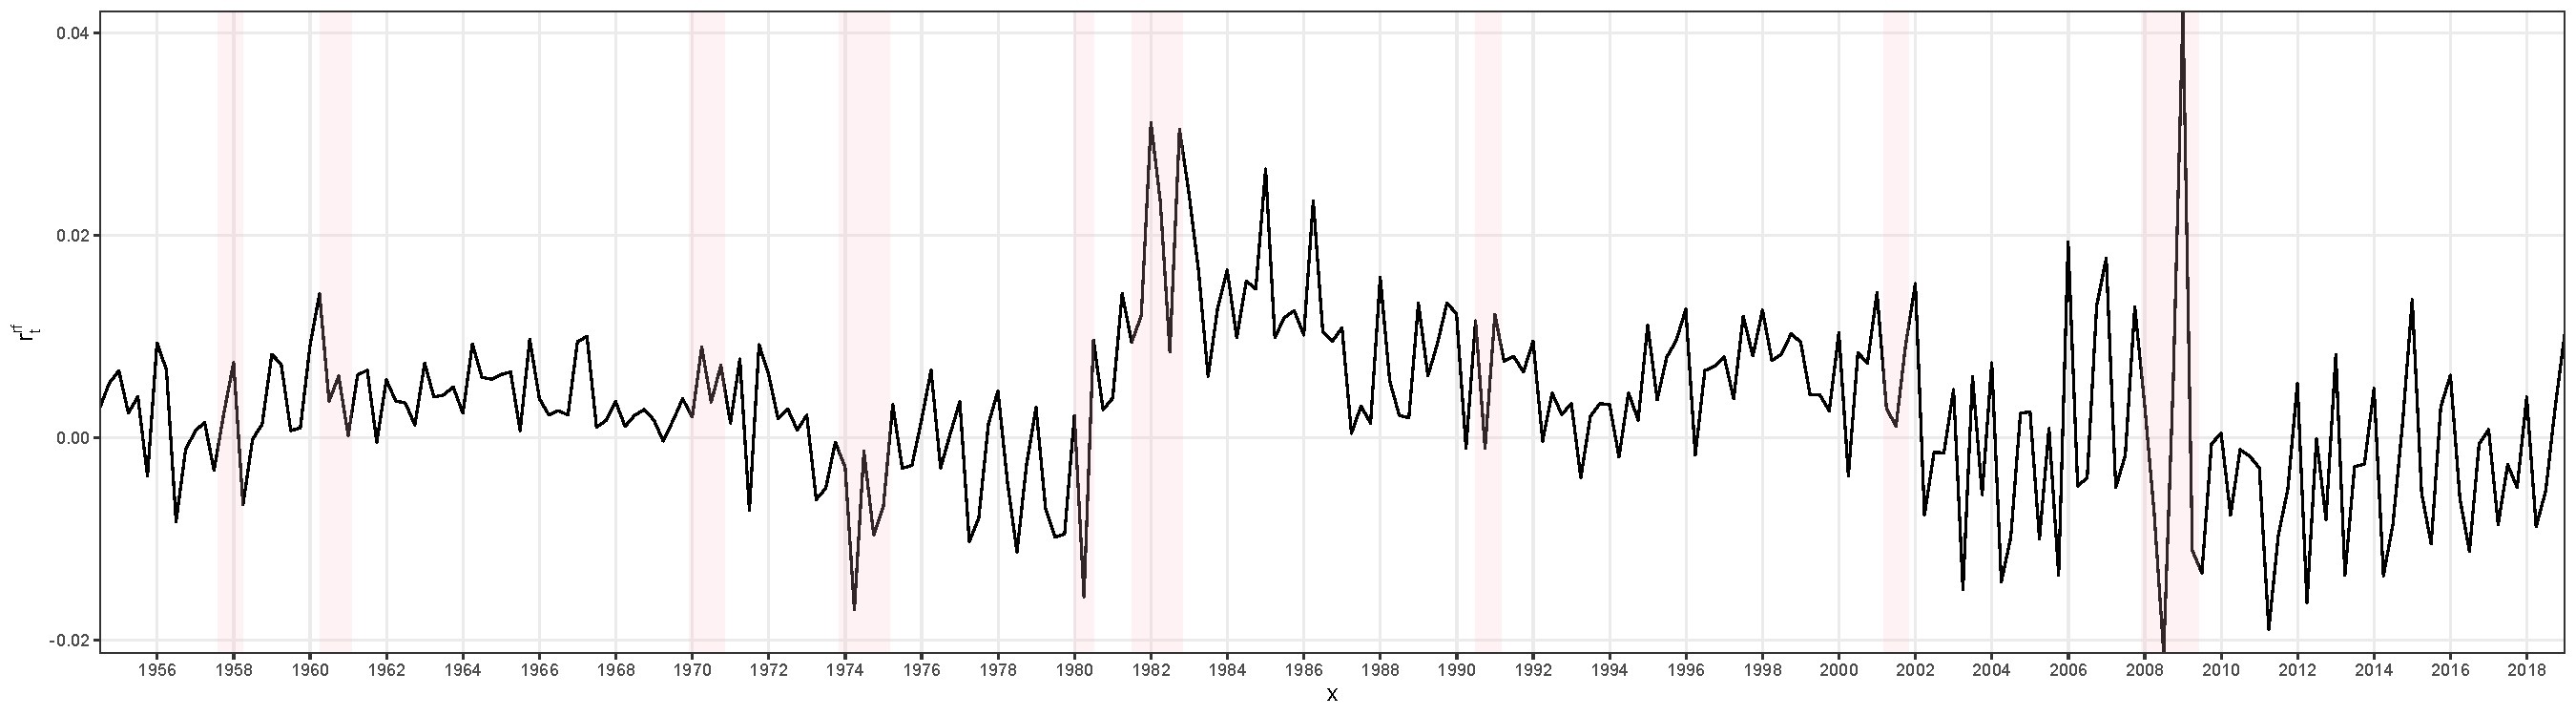
\includegraphics[width=1\linewidth]{Master_Thesis_Andreas_Kracht_Frandsen_files/figure-latex/NET-TB-tids-1} 

}

\caption[Tidsserie af log netto renten.]{Tidsserie af log netto renten.}\label{fig:NET-TB-tids}
\end{figure}

I forlængelse af beskrivelsen af det risikofrie aktiv, viser Figur \ref{fig:INF-tids} et plot over tidsserien hørende til inflationsraten.

\begin{figure}[H]

{\centering 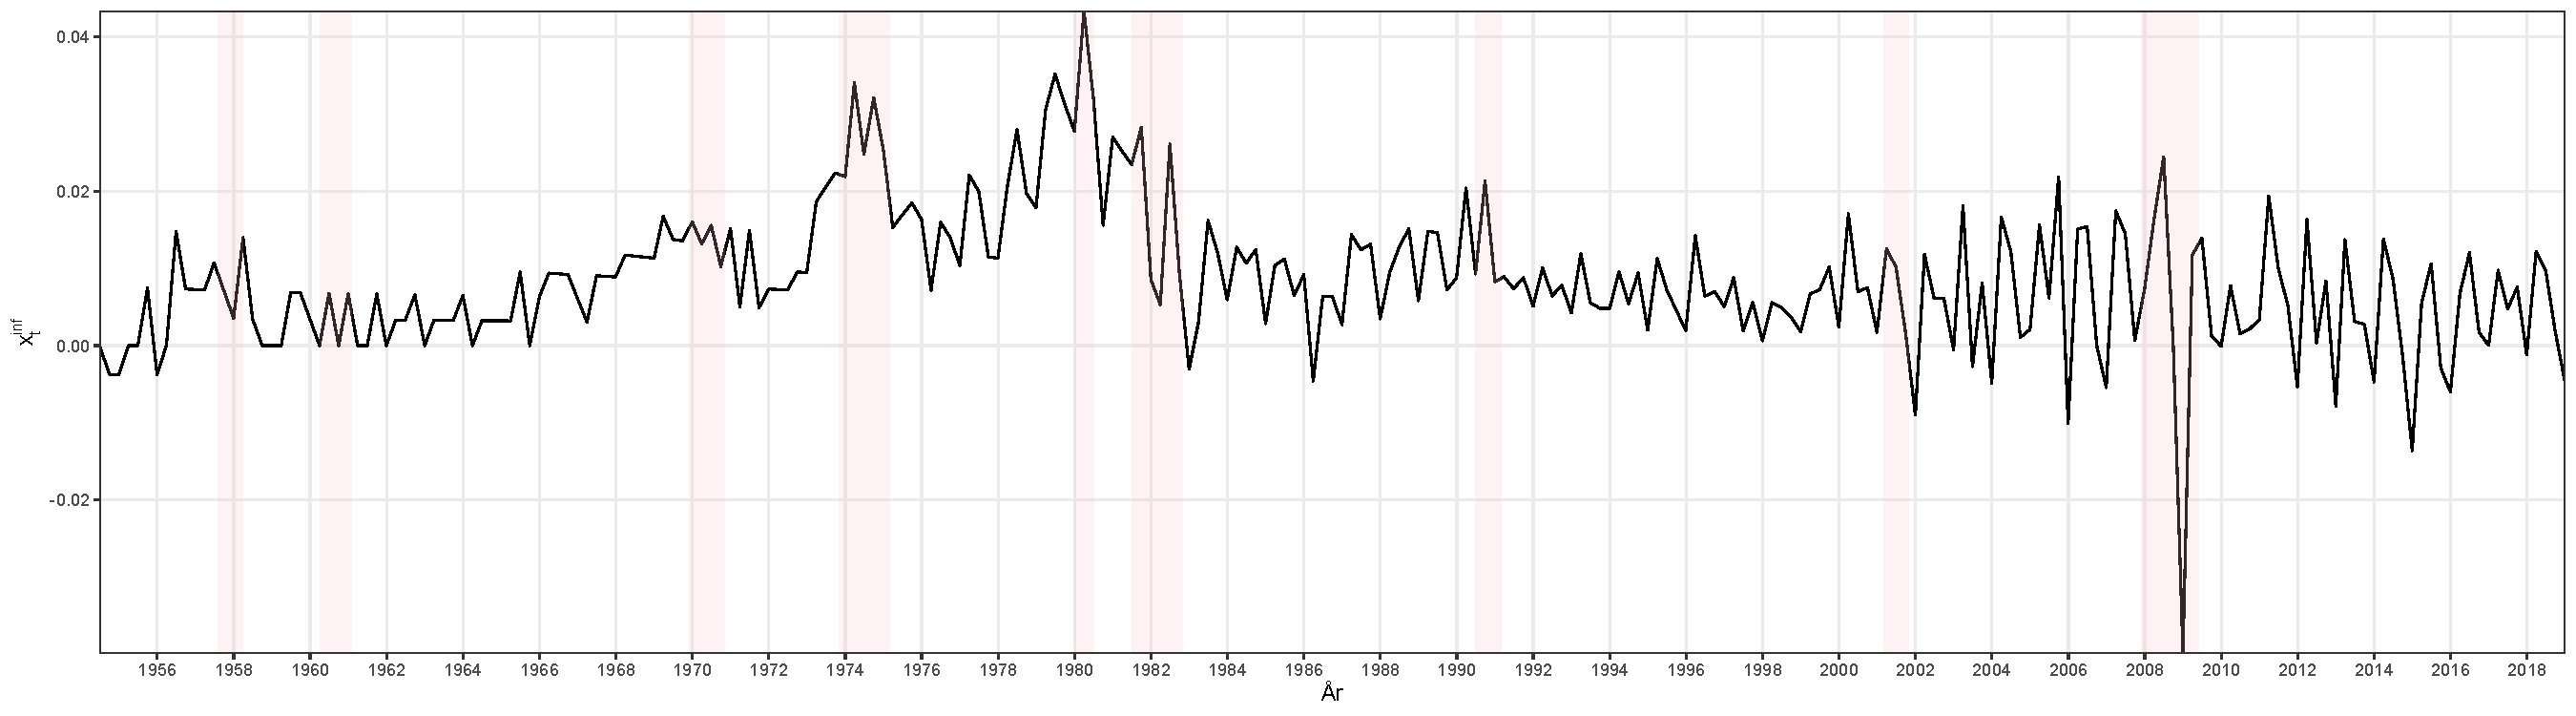
\includegraphics[width=1\linewidth]{Master_Thesis_Andreas_Kracht_Frandsen_files/figure-latex/INF-tids-1} 

}

\caption{Tidsserie af inflationsraten, målt via Consumer Price Index.}\label{fig:INF-tids}
\end{figure}

\begin{figure}[H]

{\centering 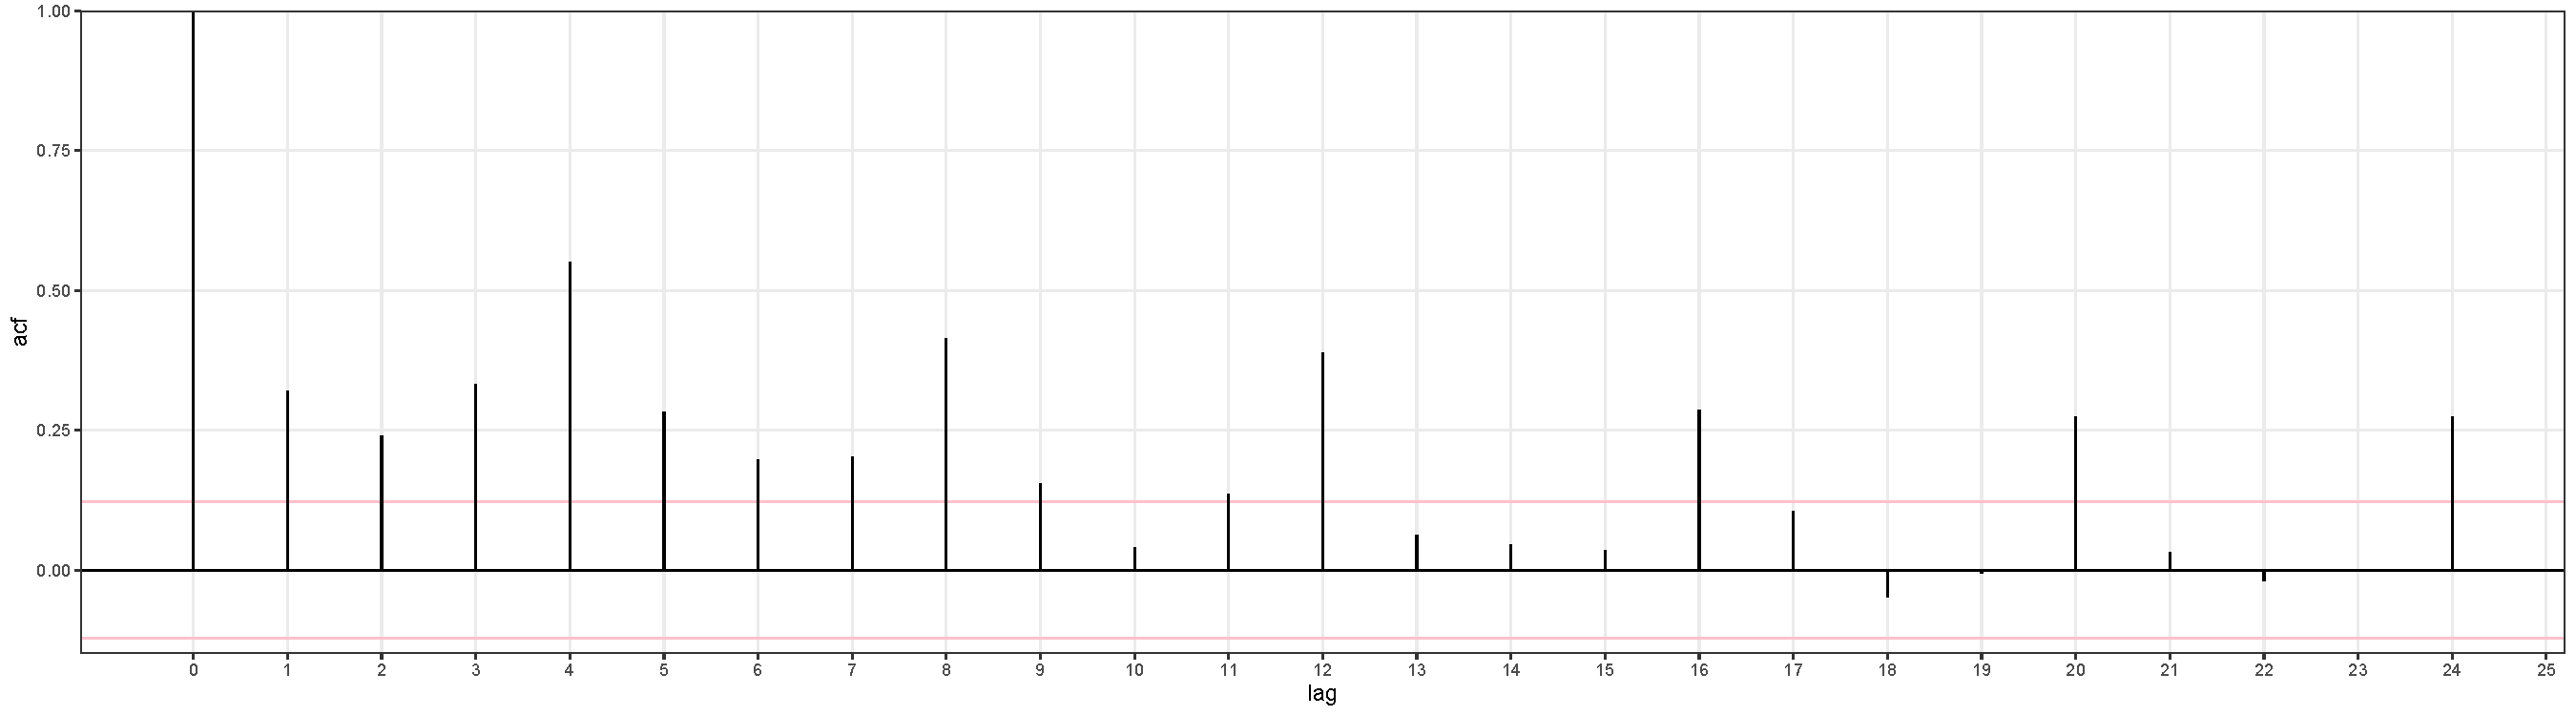
\includegraphics[width=1\linewidth]{Master_Thesis_Andreas_Kracht_Frandsen_files/figure-latex/NET-TB-AK-1} 

}

\caption{Autokorrelation af log netto renten.}\label{fig:NET-TB-AK}
\end{figure}

\begin{figure}[H]

{\centering 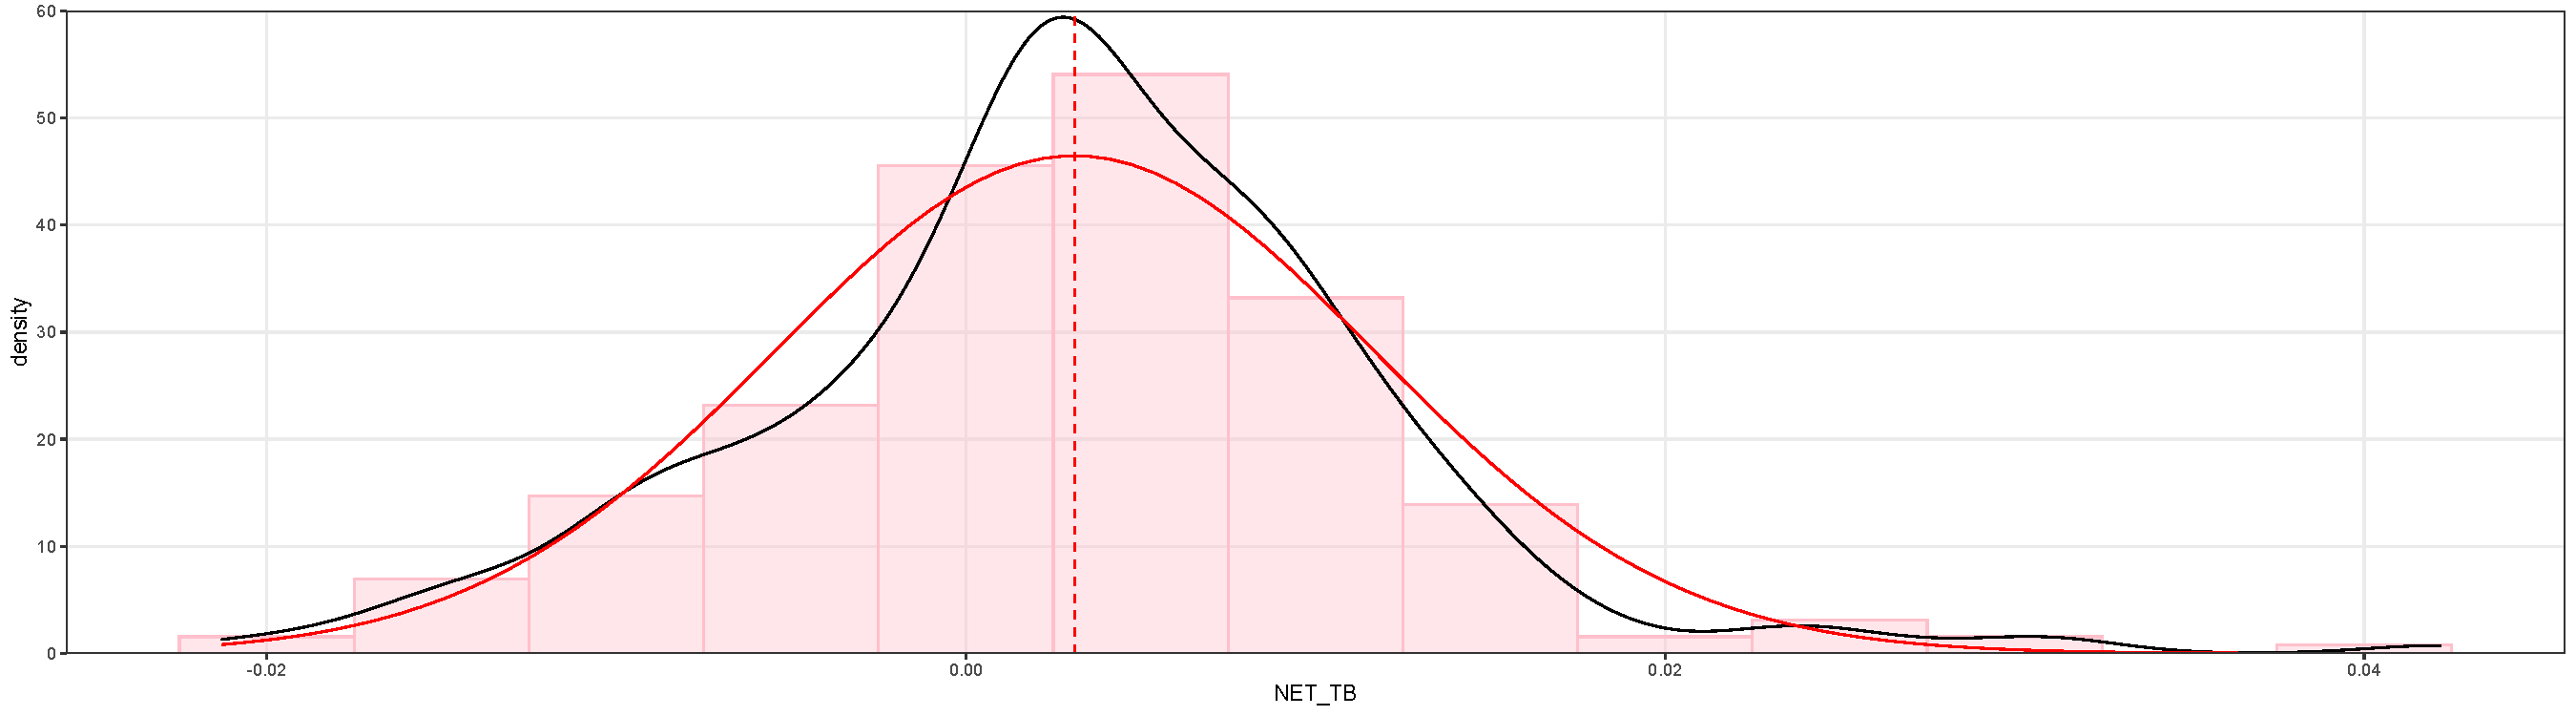
\includegraphics[width=1\linewidth]{Master_Thesis_Andreas_Kracht_Frandsen_files/figure-latex/NET-TB-HIST-1} 

}

\caption{Histogram for log netto renten.}\label{fig:NET-TB-HIST}
\end{figure}

\hypertarget{dataak}{%
\subsection{\texorpdfstring{Merafkastet på aktier -- \(rx_{t+1}^{\textnormal{a}}\)}{Merafkastet på aktier -- rx\_\{t+1\}\^{}\{\textbackslash textnormal\{a\}\}}}\label{dataak}}

For aktivklassen, som skal repræsentere børshandlede aktier, benyttes et markedsværdi-vægtet afkast over et repræsentativt indeks for samtlige handlede aktier på \emph{New York Stock Exchange}, \emph{National Association of Securities Dealers Automated Quotations} og \emph{American Stock Exchange}. Det vægtede afkast er inklusiv udbytte, aktiesplits og nyemissioner for de foregående 12 måneder ledende op til kvartalet. Ved at benytte et sådant forholdsvist bredt indeks, vil delanalysen for aktier være repræsentativt for det globale aktiemarked. Derudover er det ikke kun børsnoterede amerikanskbaserede selskaber, som handles via \emph{NYSE}, \emph{NASDAQ} og \emph{AMEX}, men i stadig større grad også virksomheder uden for U.S.A. Data over afkast er fra \citep{CRSPakt} og hentet gennem \citep{WRDSakt}. Log merafkastet af aktier beregnes som det kvartalsvise log brutto aktieafkast fratrukket det kvartalsvise brutto afkast på den amerikanske 90-dages \emph{T-Bill}. Det ses at aktier har det klart højeste kvartalvise justerede merafkast på 1.7\(\%\) ift. de andre aktivklasser. Dette høje merafkast følges af en ligeledes høj relativ volatilitet på 8.3\(\%\). Historisk set har det største negative markedsudsving givet et merafkast/tab på \(-30.4\%\), mens det største positive markedsudsving har været på \(20\%\). Et histogram sammenholdt med en skævhed på -0.946 afslører moderat til høj venstreskævhed. Altså har der oftere været negative merafkast ift. positive. Kurtosis på 4.624 medfører en moderat leptokurtisk fordeling med en anelse tykkere haler, og at ekstreme observationer sker oftere end normalt. Disse tal er konsistente med \citep{CampVic2003}. Figur \ref{fig:AKT-tids} viser et plot over tidsserien, Figur \ref{fig:AKT-AK} viser et plot over autokorrelationen for tidsserien og Figur \ref{fig:AKT-HIST} viser et plot over histogrammet for tidsserien med tilhørende \emph{kernel} tæthed samt tæthed for en normalfordelt stokastisk variabel med middelværdi og standard afvigelse lig ovenstående estimater.

\begin{figure}[H]

{\centering 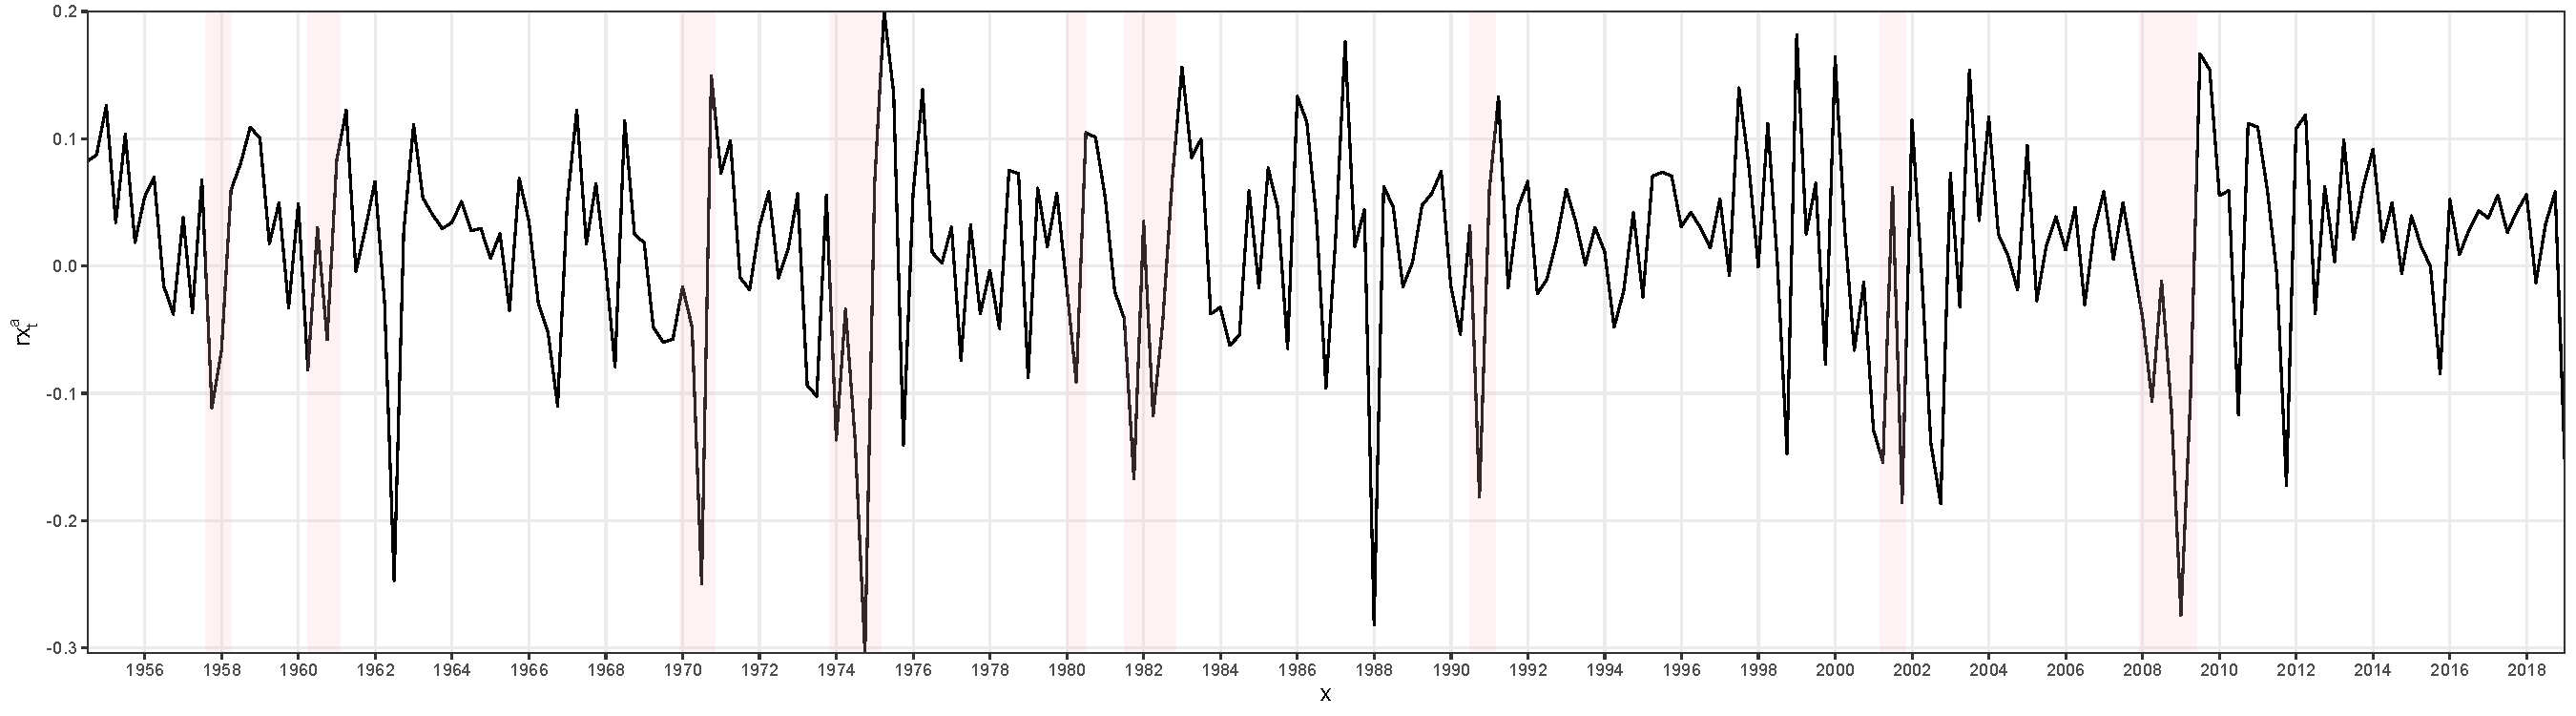
\includegraphics[width=1\linewidth]{Master_Thesis_Andreas_Kracht_Frandsen_files/figure-latex/AKT-tids-1} 

}

\caption{Tidsserie af log merafkastet af aktier.}\label{fig:AKT-tids}
\end{figure}

\begin{figure}[H]

{\centering 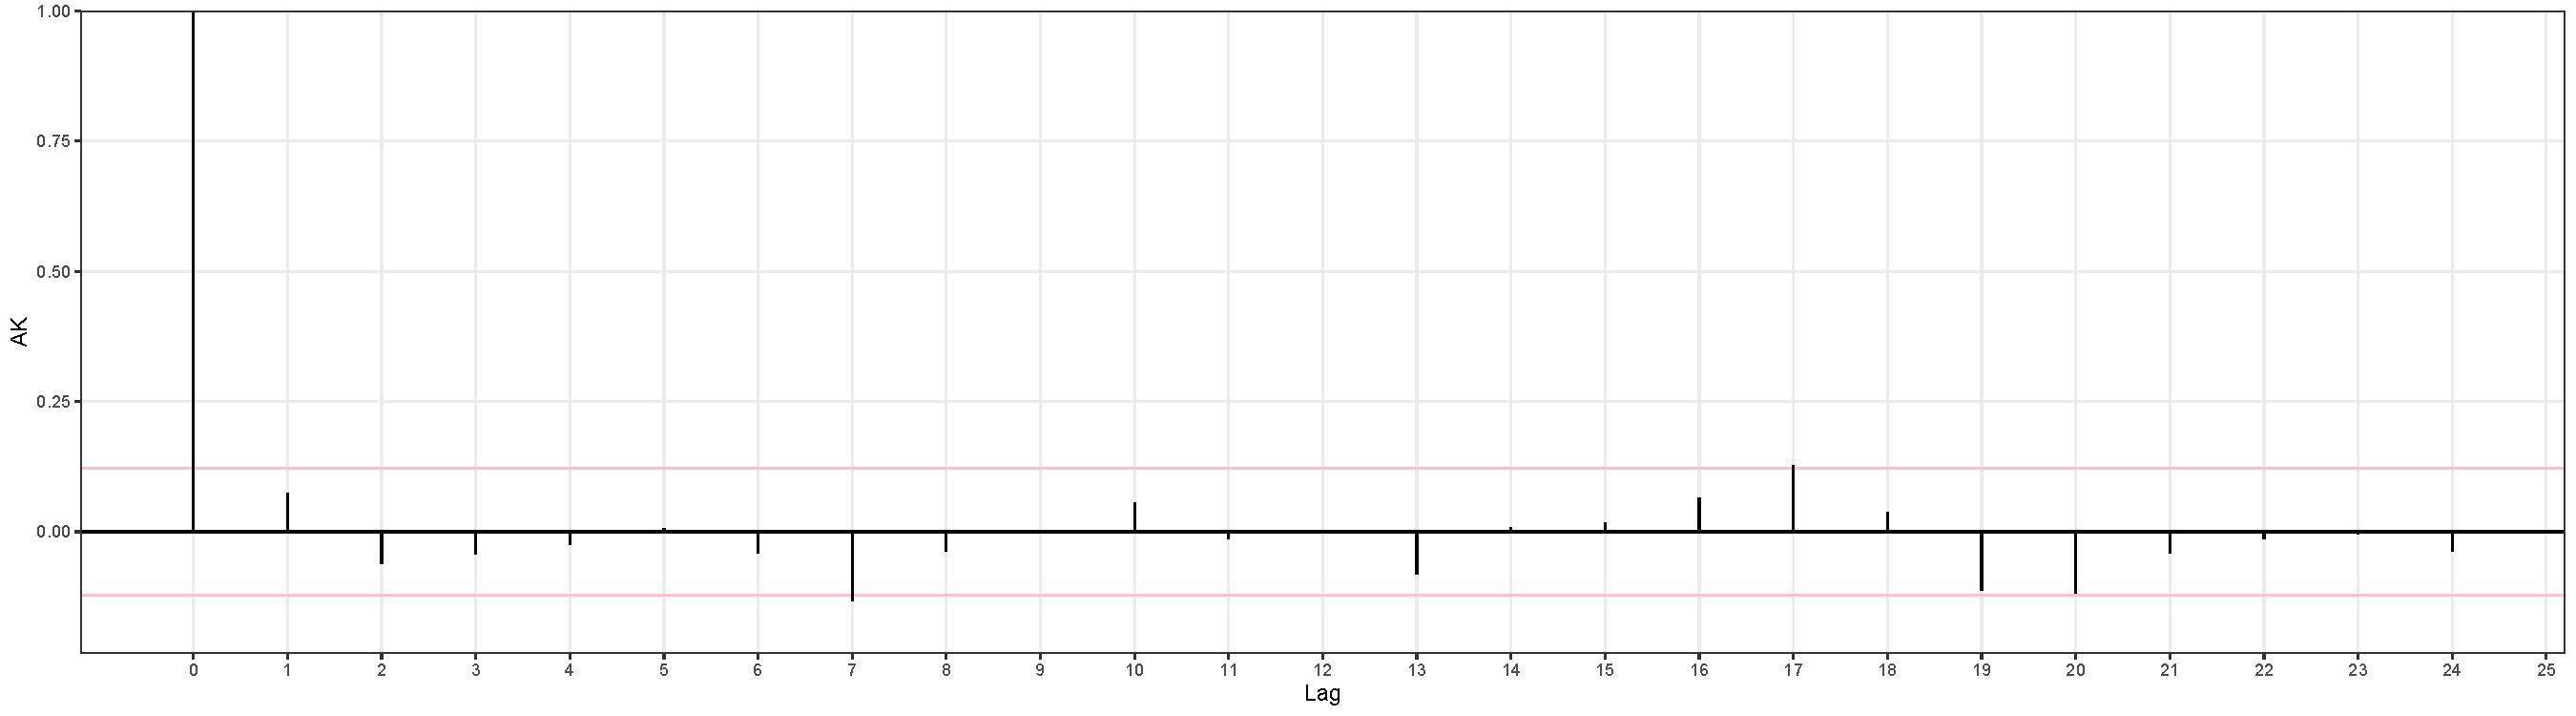
\includegraphics[width=1\linewidth]{Master_Thesis_Andreas_Kracht_Frandsen_files/figure-latex/AKT-AK-1} 

}

\caption{Autokorrelation af log merafkastet af aktier.}\label{fig:AKT-AK}
\end{figure}

\begin{figure}[H]

{\centering 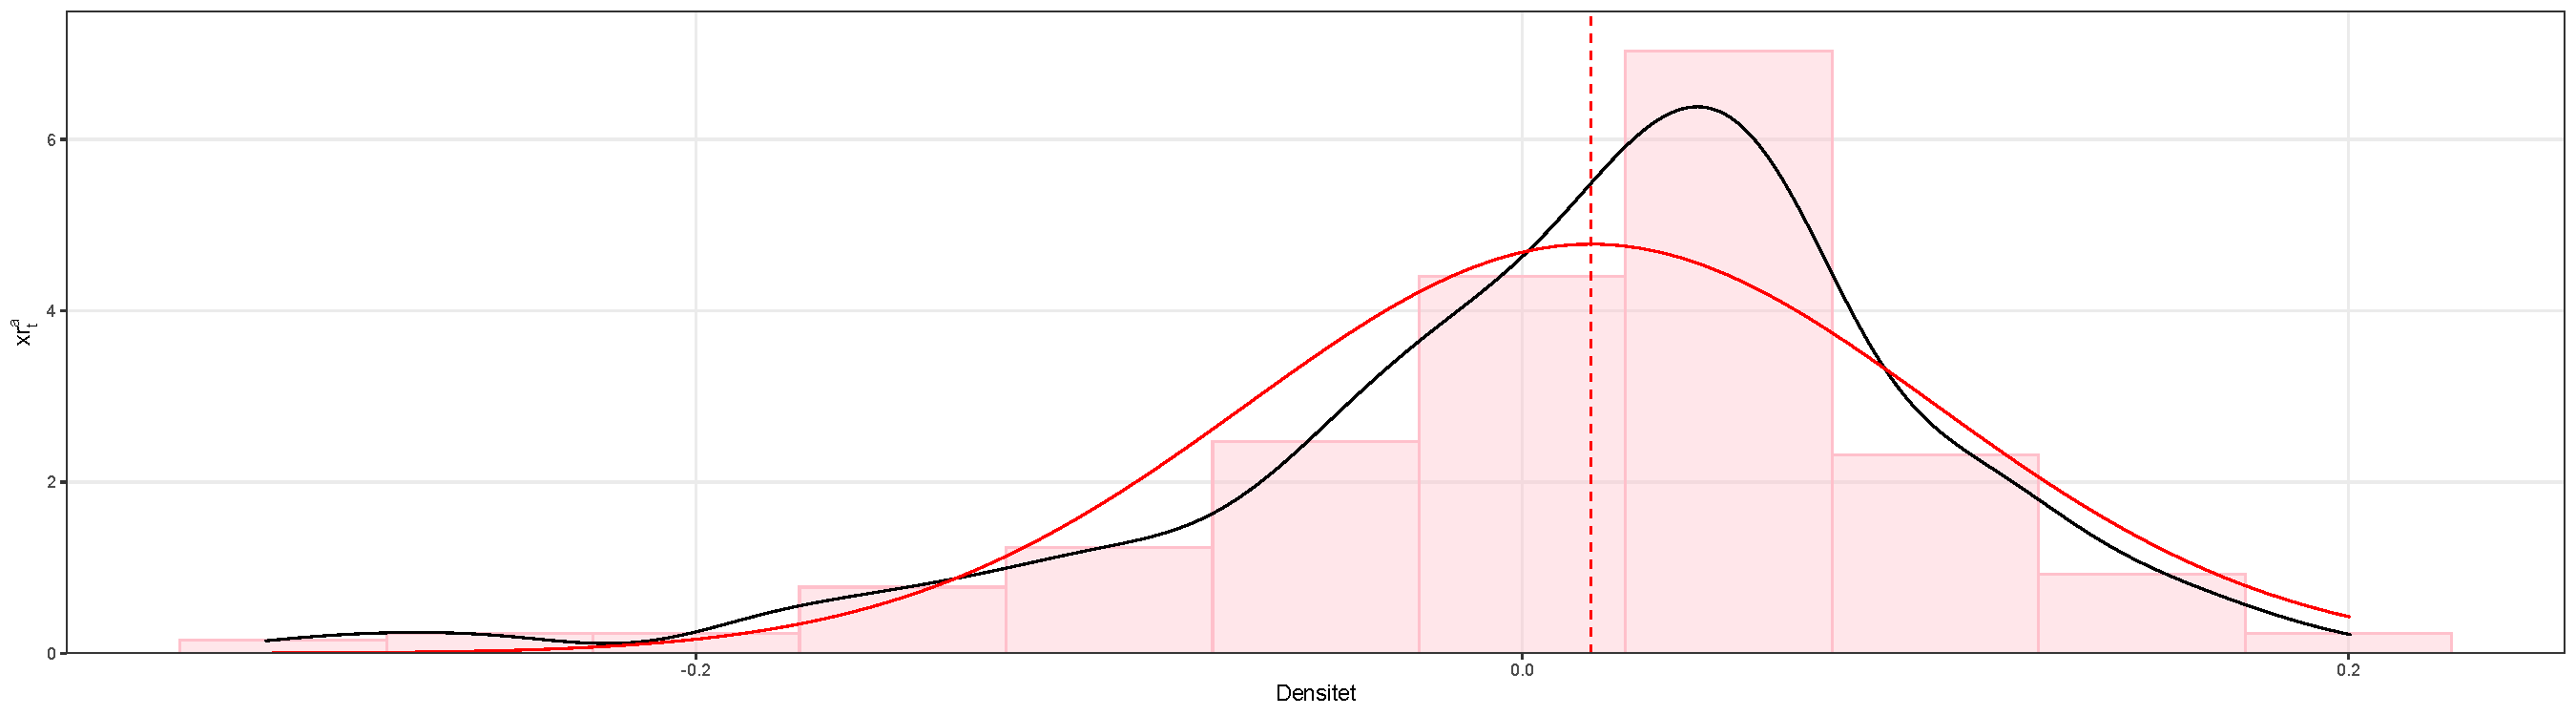
\includegraphics[width=1\linewidth]{Master_Thesis_Andreas_Kracht_Frandsen_files/figure-latex/AKT-HIST-1} 

}

\caption{Histogram for log merafkastet af aktier.}\label{fig:AKT-HIST}
\end{figure}

\hypertarget{merafkastet-puxe5-statsobligationer-rx_t1textnormals}{%
\subsection{\texorpdfstring{Merafkastet på statsobligationer -- \(rx_{t+1}^{\textnormal{s}}\)}{Merafkastet på statsobligationer -- rx\_\{t+1\}\^{}\{\textbackslash textnormal\{s\}\}}}\label{merafkastet-puxe5-statsobligationer-rx_t1textnormals}}

Statsobligationer er gældsinstrumenter udstedt af staten i det respektive udstedelsesland, de har til formål at finansiere offentlige udgifter og anses også for at være en substitution for skatter. Siden udstedelsen sker af staten, antages det ofte, at statsobligationer er relativt mindre risikobærende and aktier. Undertiden betegnes statsobligationer fra visse ilande som et \emph{safe haven} for investorer. Eksempelvis har den danske stat pt.~en kreditvurdering på AAA, Aaa, AAA af hhv. \emph{Standard \& Poor's}, \emph{Moody's} og \emph{Fitch}, \citep{TradingEconomics2020}. Til formålet at repræsentere afkastet på statsobligationer anvendes derfor den 10-årige amerikanske statsobligation med konstant løbetid. Data over afkast er fra \citep{CRSPt90} og hentet gennem \citep{WRDSt90}. Log merafkastet af statsobligationener beregnes som det kvartalsvise log brutto afkast fratrukket det kvartalsvise brutto afkast på den amerikanske 90-dages \emph{T-Bill}. merafkastet har et justeret kvartalsvist afkast på 0.3\(\%\) med en kvartalsvis volatilitet på 3.8\(\%\). Statsobligationen har den laveste \emph{Sharpe Ratio} af de tre aktivklasser, hvilket også er forventeligt. Med en skævhed på 0.451 og kurtosis på 3.405 haves en forholdsvis symmetrisk fordeling, men med en anelse tykkere haler. Disse tal er konsistente med \citep{CampVic2003}. Figur \ref{fig:S-OBL-tids} viser et plot over tidsserien, Figur \ref{fig:S-OBL-AK} viser et plot over autokorrelationen for tidsserien og Figur \ref{fig:S-OBL-HIST} viser et plot over histogrammet for tidsserien med tilhørende \emph{kernel} tæthed samt tæthed for en normalfordelt stokastisk variabel med middelværdi og standard afvigelse lig ovenstående estimater.

\begin{figure}[H]

{\centering 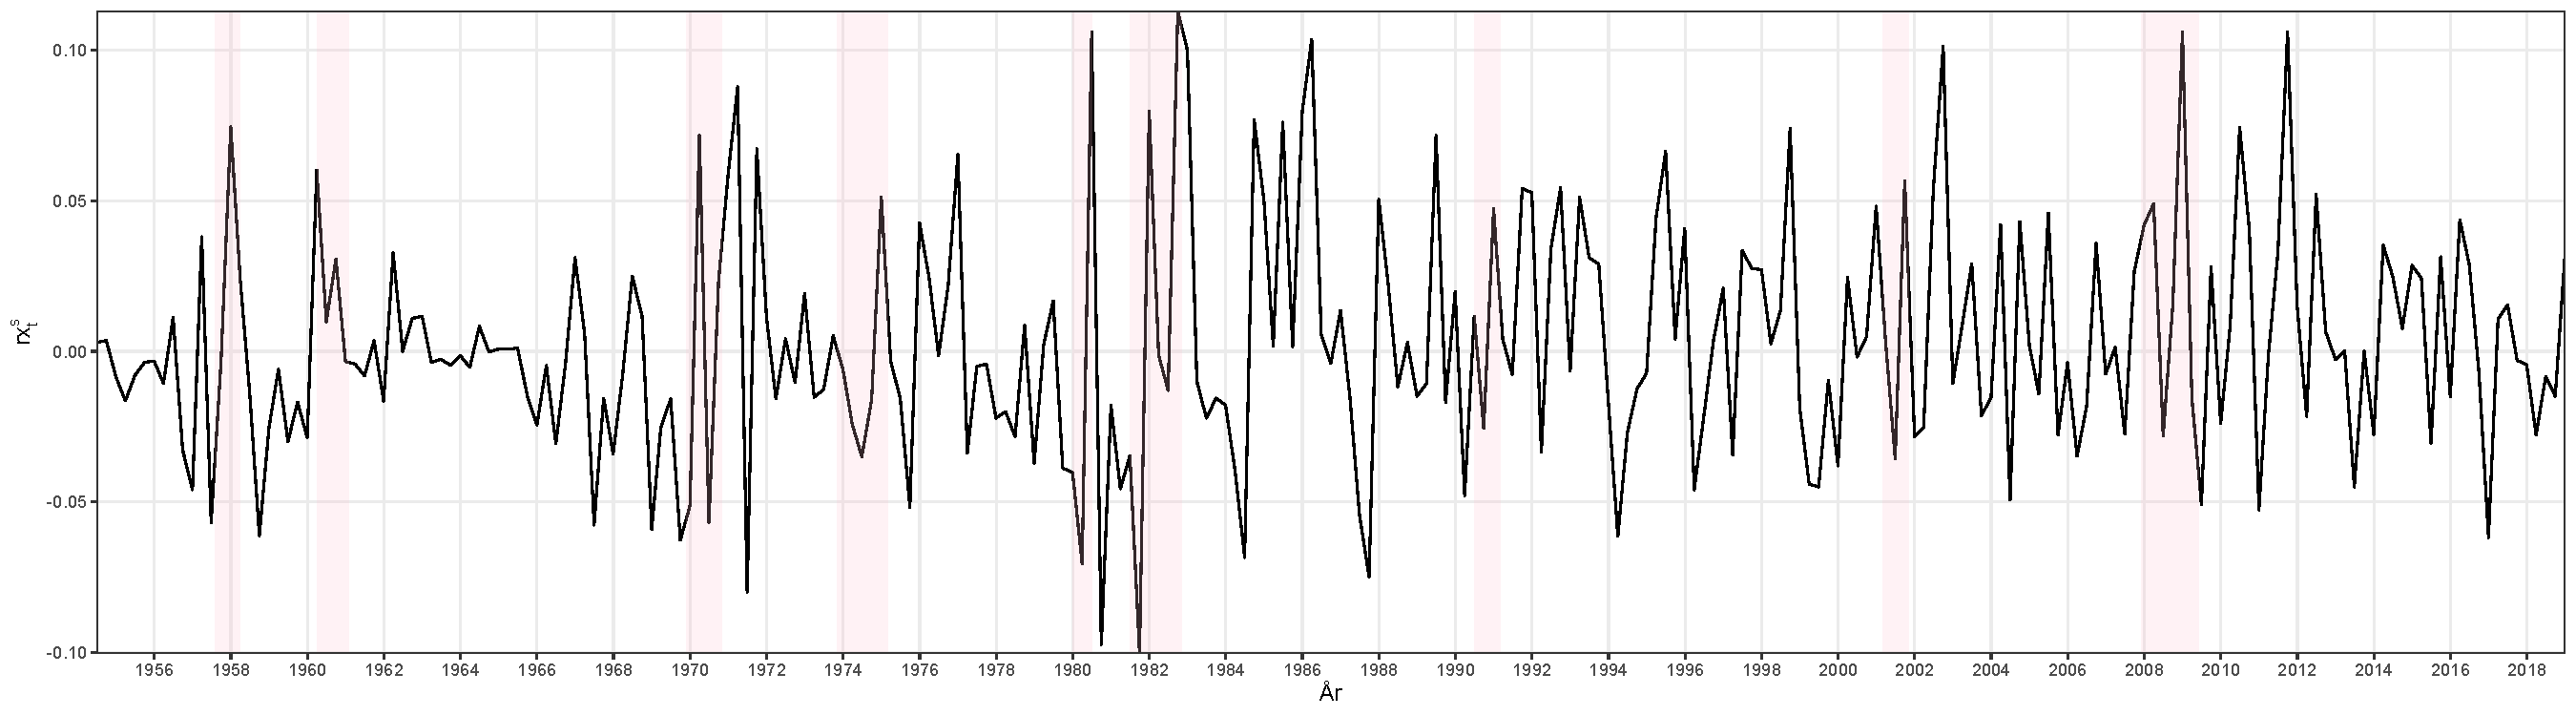
\includegraphics[width=1\linewidth]{Master_Thesis_Andreas_Kracht_Frandsen_files/figure-latex/S-OBL-tids-1} 

}

\caption{Tidsserie af log merafkastet på statsobligationer.}\label{fig:S-OBL-tids}
\end{figure}

\begin{figure}[H]

{\centering 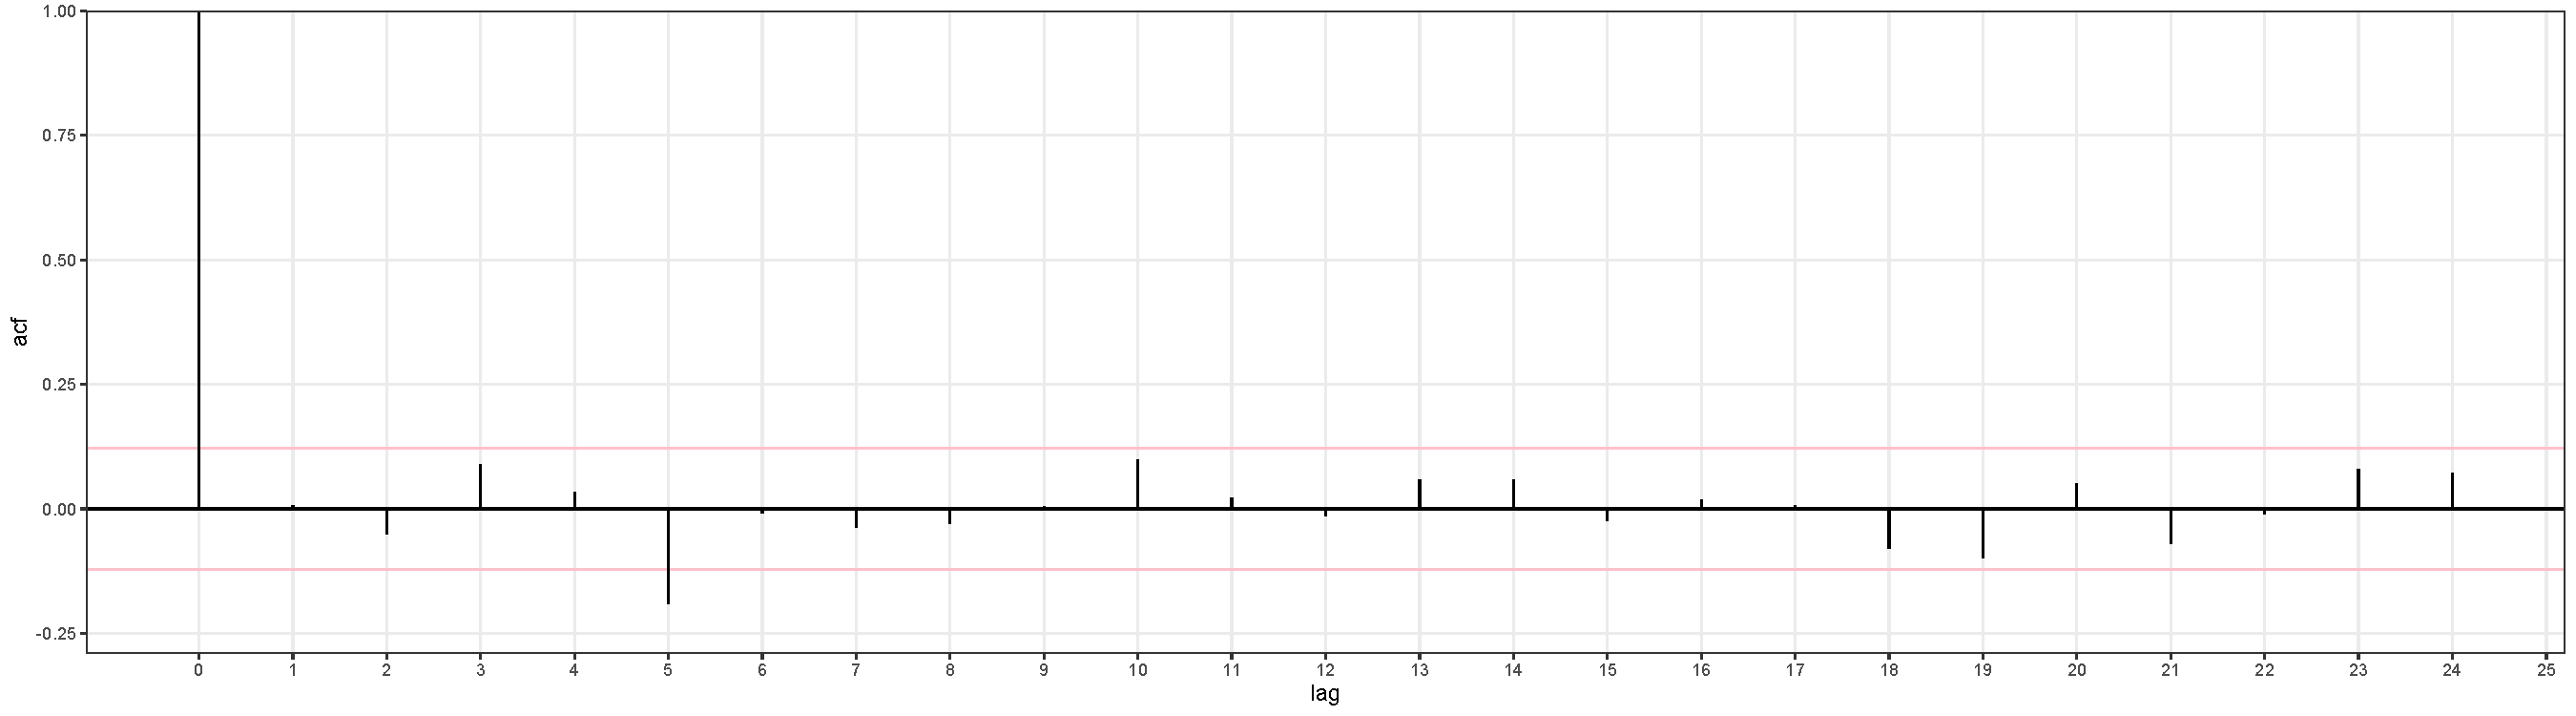
\includegraphics[width=1\linewidth]{Master_Thesis_Andreas_Kracht_Frandsen_files/figure-latex/S-OBL-AK-1} 

}

\caption{Autokorrelation af log merafkastet af statsobligationer.}\label{fig:S-OBL-AK}
\end{figure}

\begin{figure}[H]

{\centering 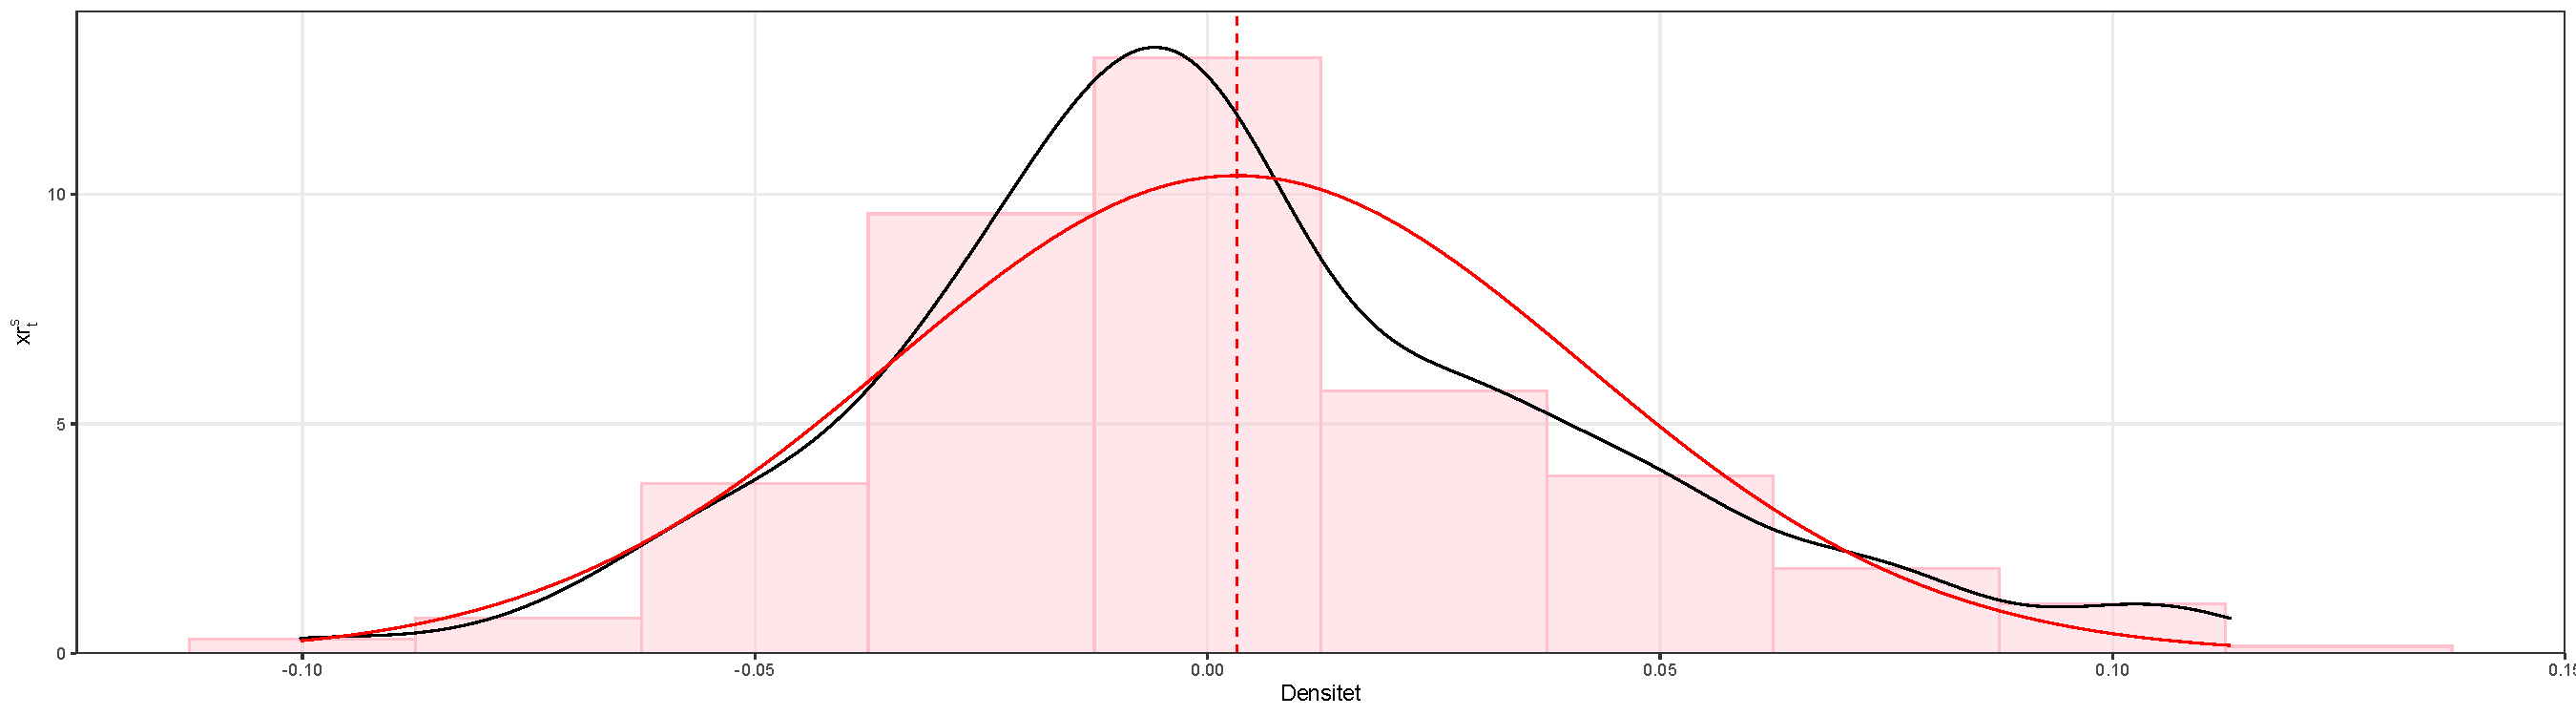
\includegraphics[width=1\linewidth]{Master_Thesis_Andreas_Kracht_Frandsen_files/figure-latex/S-OBL-HIST-1} 

}

\caption{Histogram for log merafkastet på statsobligationer.}\label{fig:S-OBL-HIST}
\end{figure}

\hypertarget{merafkastet-puxe5-virksomhedsobligationer-rx_t1textnormalv}{%
\subsection{\texorpdfstring{Merafkastet på virksomhedsobligationer -- \(rx_{t+1}^{\textnormal{v}}\)}{Merafkastet på virksomhedsobligationer -- rx\_\{t+1\}\^{}\{\textbackslash textnormal\{v\}\}}}\label{merafkastet-puxe5-virksomhedsobligationer-rx_t1textnormalv}}

På samme vis som stater kan finansiere deres aktiviteter via statsobligationer, kan virksomheder udstede gæld via obligationer, hvis formål er at finansiere fremtidige investeringer og/eller projekter. Sikkerheden bag en virksomhedsobligation afhænger af virksomhedens betalingsevne. Af og til sætter virksomheden fysiske aktiver som kollateral for obligationerne i tilfælde af konkurser. Ift. statsobligationer bærer virksomhedsobligationer på en langt større risiko givet kreditrisikoen i virksomheden og/eller markedet. For at påtage sig denne risiko, forlanger investorerne derfor en højere præmie i form af en højere rente tilhørende virksomhedsobligationerne. For at repræsentere virksomhedsobligationer anvendes en indeksserie af virksomhedsobligationer med lang løbetid. Data er fra \citep{Ibbotson2019} og hentet via \citep{Goyal2007}\footnote{Mere specifickt via \emph{Amit Goyals} hjemmeside, hvor der findes en opdateret version af dataet, som der benyttes i artiklen, se evt. \citep{Goyal2020}.}. Det specifikke grundlag for tidsserien er tvetydigt, men \citep{Ibbotson2019} skriver følgende.

\begin{center}
\textit{A corporate bond series with a long maturity is used to describe fixed-income securities that contain risk of default.}
\end{center}

Log merafkastet af virksomhedsobligationenerne beregnes som det kvartalsvise log brutto afkast fratrukket det kvartalsvise brutto afkast på den amerikanske 90-dages \emph{T-Bill}. Som forventet ses den højere afkastpræmie med et justeret kvartalsvist afkast på 0.5\(\%\) og en tilhørende volatilitet på 4.7\(\%\), som investoren får, for at påtage sig den ekstra kreditrisiko. Afkastfordelingen anses som værende relativt mest symmetrisk ift. de andre aktivklasser, hvilket også ses i en skævhedsværdi på 0.216. Med en kurtosis på mere end \(3\), har fordelingen tykkere haler og med mere masse centralt i fordelingen. Det bemærkes ligeledes at virksomhedsobligationer har haft de største positive markedsudsving af de tre aktivklasser med et positivt afkast på \(20.8 \%\). Figur \ref{fig:V-OBL-tids} viser et plot over tidsserien, Figur \ref{fig:V-OBL-AK} viser et plot over autokorrelationen for tidsserien og Figur \ref{fig:V-OBL-HIST} viser et plot over histogrammet for tidsserien med tilhørende \emph{kernel} tæthed samt tæthed for en normalfordelt stokastisk variabel med middelværdi og standard afvigelse lig ovenstående estimater.

\begin{figure}[H]

{\centering 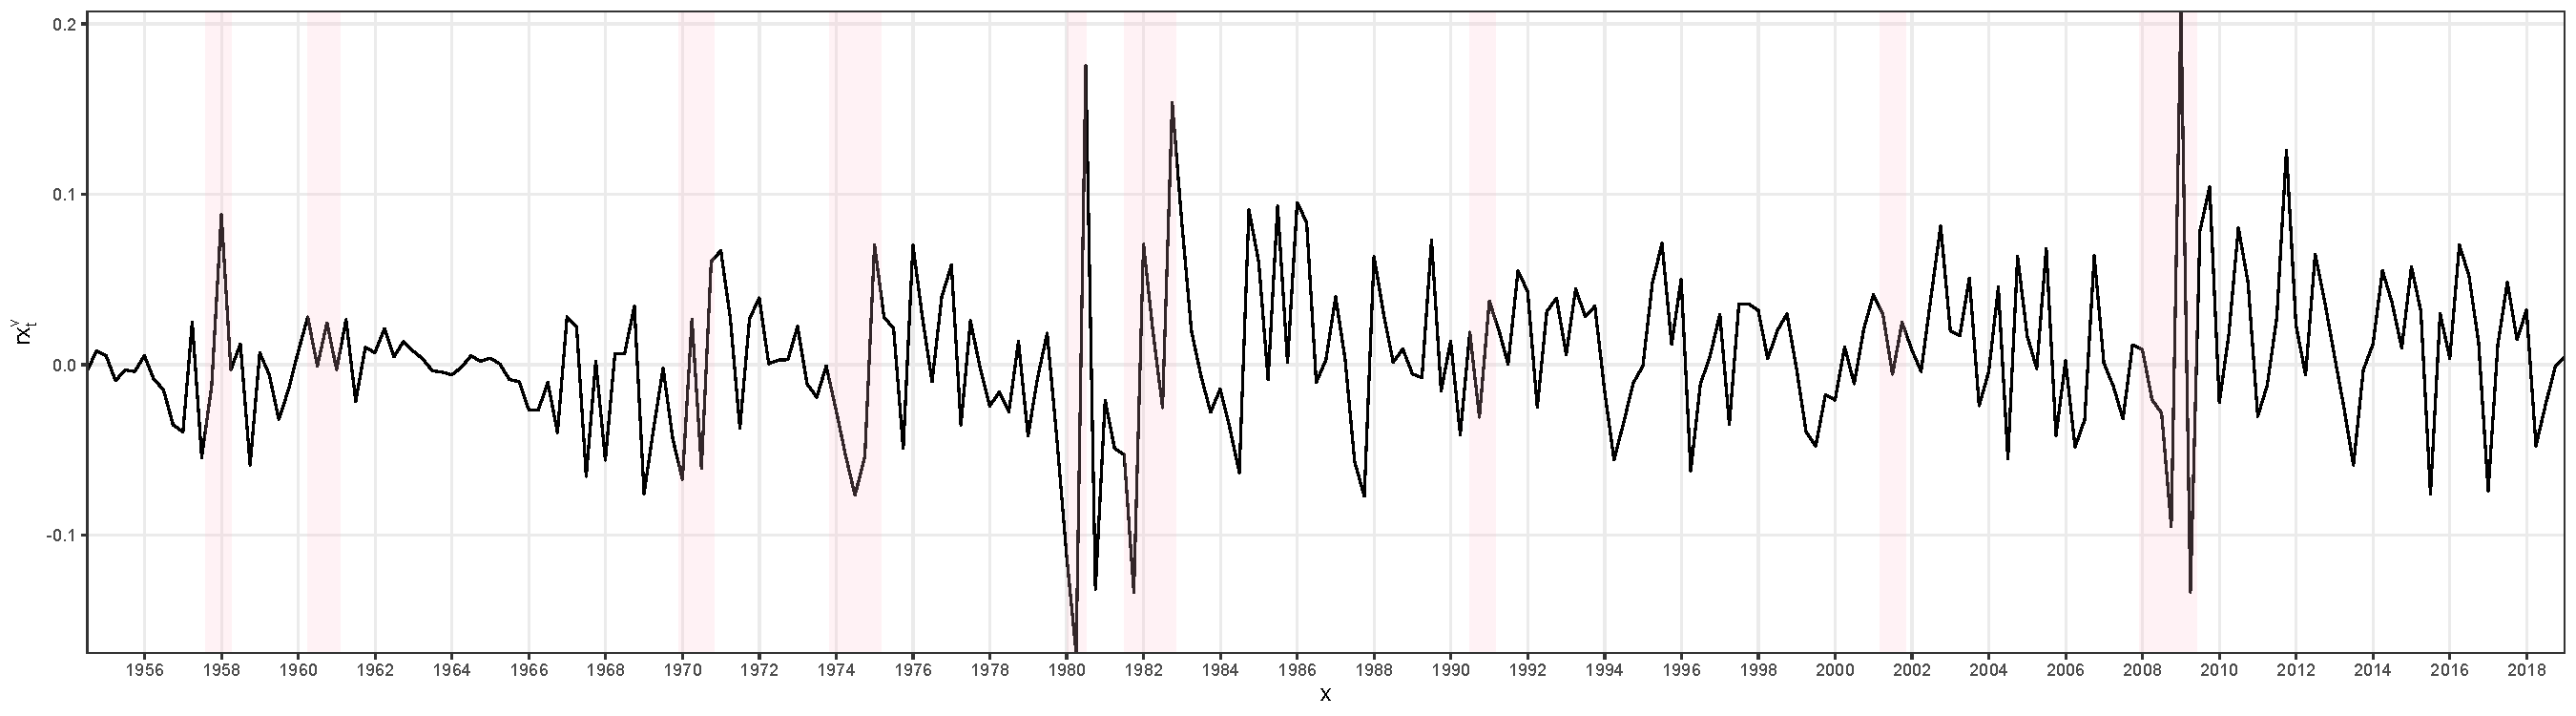
\includegraphics[width=1\linewidth]{Master_Thesis_Andreas_Kracht_Frandsen_files/figure-latex/V-OBL-tids-1} 

}

\caption{Tidsserie af log merafkastet på virksomhedsobligationer.}\label{fig:V-OBL-tids}
\end{figure}

\begin{figure}[H]

{\centering 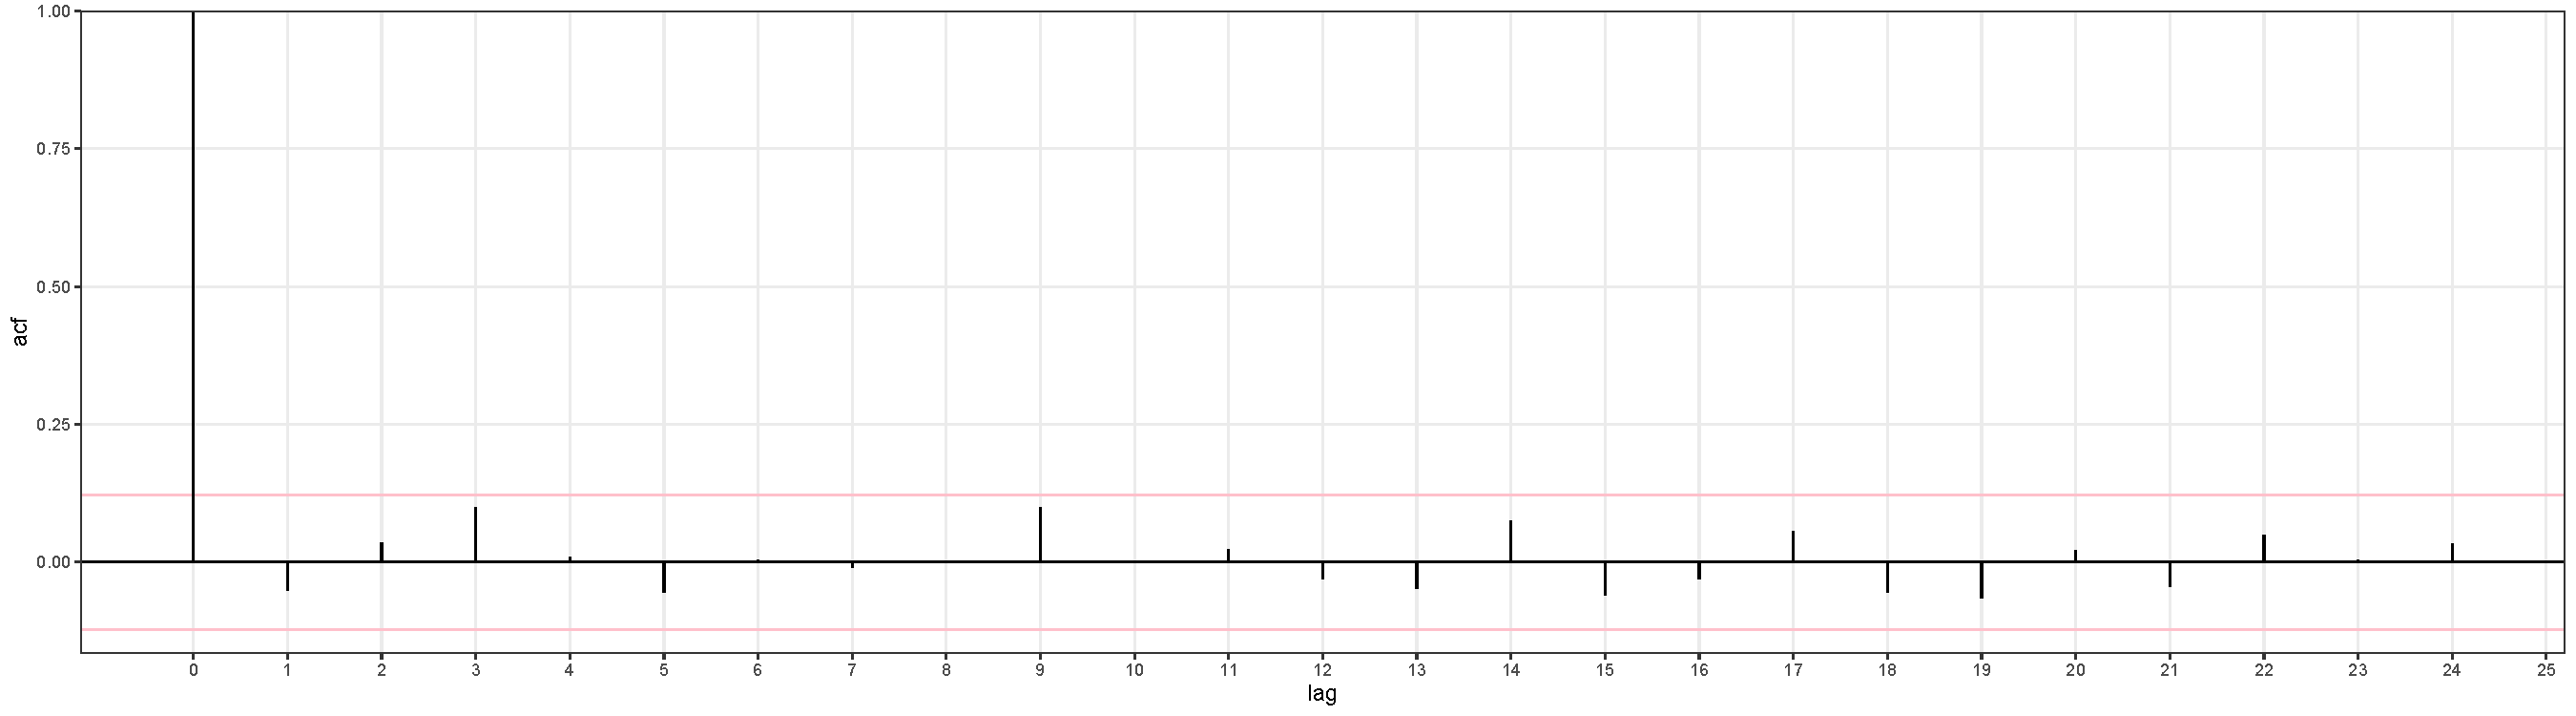
\includegraphics[width=1\linewidth]{Master_Thesis_Andreas_Kracht_Frandsen_files/figure-latex/V-OBL-AK-1} 

}

\caption{Autokorrelation af log merafkastet af virksomhedsobligationer.}\label{fig:V-OBL-AK}
\end{figure}

\begin{figure}[H]

{\centering 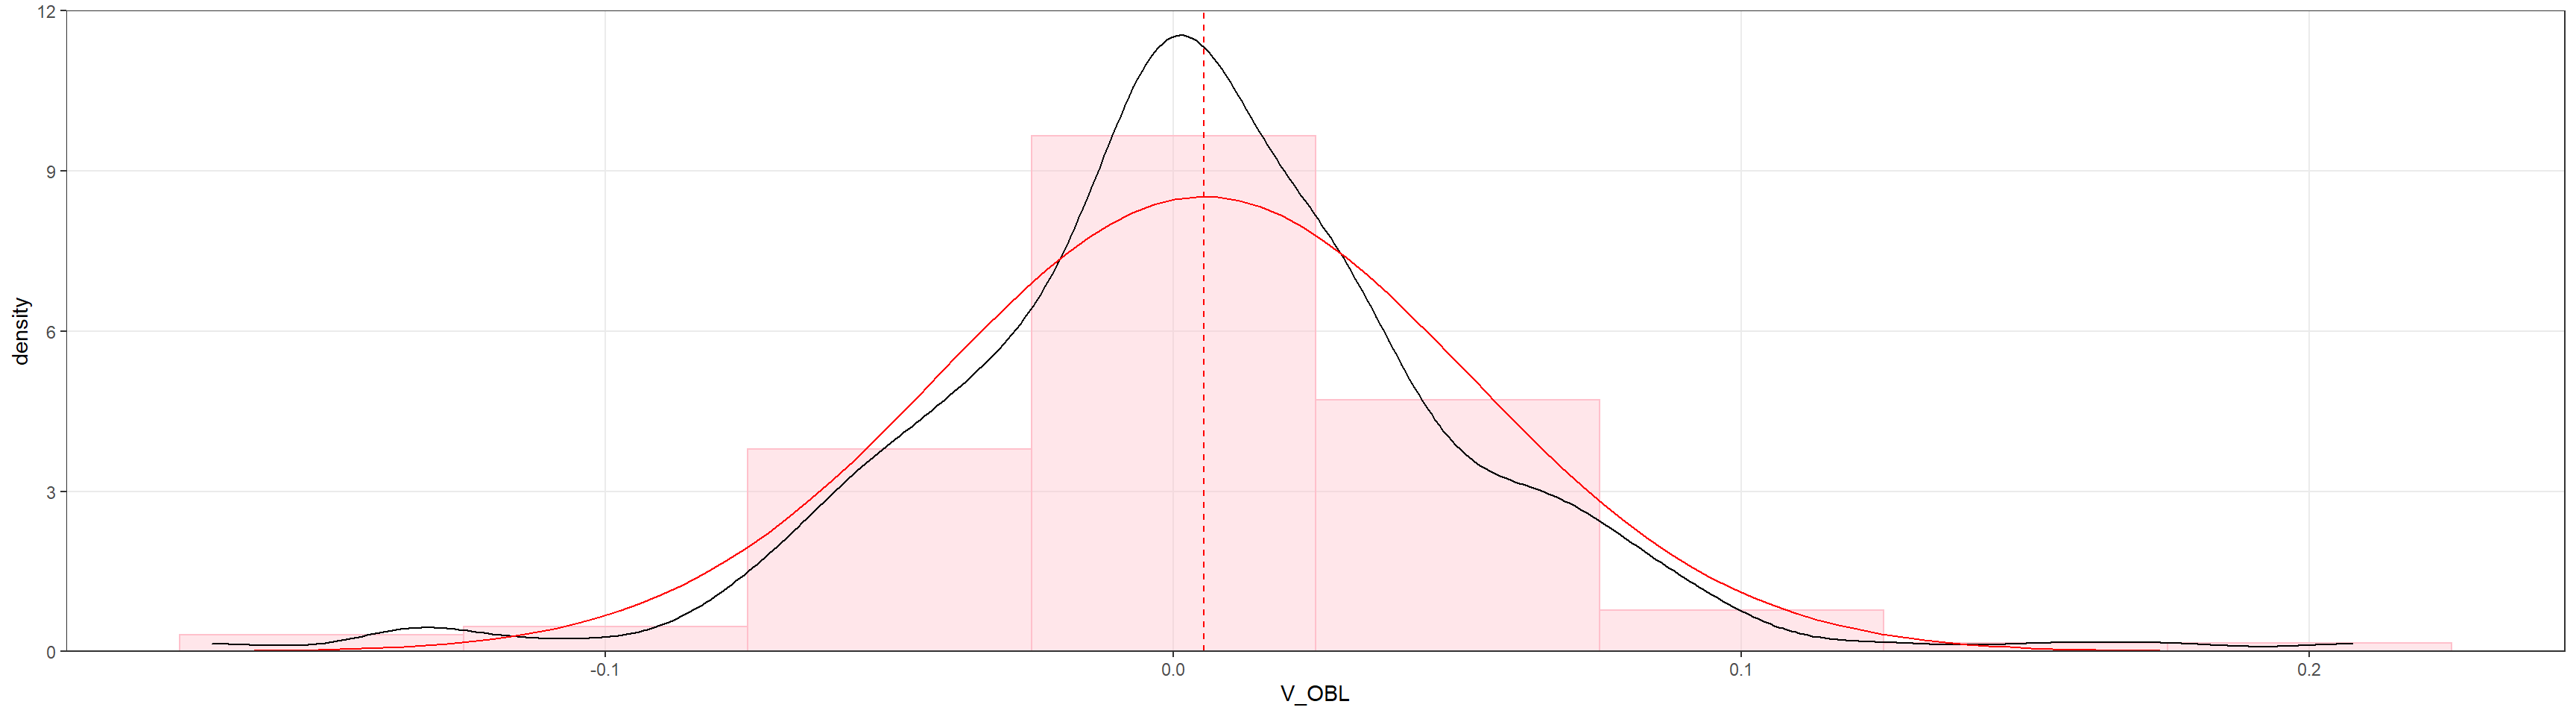
\includegraphics[width=1\linewidth]{Master_Thesis_Andreas_Kracht_Frandsen_files/figure-latex/V-OBL-HIST-1} 

}

\caption{Histogram for log merafkastet på virksomhedsobligationer.}\label{fig:V-OBL-HIST}
\end{figure}

Tabel \ref{tab:DES-AKTIVKLASSE} opsummerer ovenstående beskrivende statistik for de fire aktivkasser.



\begin{table}[H]

\caption{\label{tab:DES-AKTIVKLASSE}Beskrivende statistik for de fire aktivklasser.}
\centering
\resizebox{\linewidth}{!}{
\begin{threeparttable}
\begin{tabular}[t]{lrrrrrrrrrrr}
\toprule
  & Middelværdi & Standard afvigelse & Sharpe Ratio & Skævhed & Kurtosis & Minimum & $25 \%$ & Median & $75 \%$ & Maksimum & AK(1)\\
\midrule
\rowcolor{gray!6}  $r_t^{\text{rf}}$ & 0.003 & 0.009 &  & 0.362 & 5.016 & -0.021 & -0.001 & 0.003 & 0.008 & 0.042 & 0.320\\
$rx_t^{\text{a}}$ & 0.017 & 0.083 & 0.199 & -0.946 & 4.624 & -0.304 & -0.028 & 0.029 & 0.062 & 0.200 & 0.075\\
\rowcolor{gray!6}  $rx_t^{\text{s}}$ & 0.003 & 0.038 & 0.084 & 0.451 & 3.405 & -0.100 & -0.021 & -0.003 & 0.025 & 0.113 & 0.007\\
$rx_t^{\text{v}}$ & 0.005 & 0.047 & 0.114 & 0.216 & 5.588 & -0.169 & -0.021 & 0.003 & 0.028 & 0.208 & -0.051\\
\bottomrule
\end{tabular}
\begin{tablenotes}
\item \textit{Denne tabel rapporterer kvartalsvis beskrivende statistik for aktivklasserne: det risikofrie aktiv, merafkastet på aktier, merafkastet på statsobligationer og merafkastet på virksomhedsobligationer. Dette gøres ud fra $259$ kvartalvise observationer, som spænder over kvartalerne fra 2. kvartal 1954 til 4. kvartal 2018. Middelværdien er justeret for alle aktivklasser.}
\end{tablenotes}
\end{threeparttable}}
\end{table}

\begin{table}[H]

\caption{\label{tab:JB-AKTIVKLASSE}Jarque-Bera test.}
\centering
\begin{threeparttable}
\begin{tabular}[t]{lrr}
\toprule
  & Teststørrelse & $p$-værdi\\
\midrule
\rowcolor{gray!6}  $r_t^{\text{rf}}$ & 49.509 & 0.000\\
$rx_t^{\text{a}}$ & 67.131 & 0.000\\
\rowcolor{gray!6}  $rx_t^{\text{s}}$ & 10.545 & 0.005\\
$rx_t^{\text{v}}$ & 74.307 & 0.000\\
\bottomrule
\end{tabular}
\begin{tablenotes}
\item \textit{Denne tabel rapporterer Jarque-Beta teststørrelser og $p$-værdier for aktivklasserne: det risikofrie aktiv, merafkastet på aktier, merafkastet på statsobligationer og merafkastet på virksomhedsobligationer, \citep{Jarque1980}. Dette gøres ud fra $259$ kvartalvise observationer, som spænder over kvartalerne fra 2. kvartal 1954 til 4. kvartal 2018.}
\end{tablenotes}
\end{threeparttable}
\end{table}

\hypertarget{pvariable}{%
\section{Prædiktionsvariable}\label{pvariable}}

Denne sektion har til formål at beskrive datagrundlaget for prædiktionsvariablene, som først blev beskrevet i Sektion \ref{potpradik}. Disse variable består af en række finansielle indikatorer: \emph{Dividend-Price Ratio}, \emph{Price-Earnings Ratio}, \emph{Book-to-market Ratio}, \emph{High Minus Low}, \emph{Small Minus Big}, og variansen af aktieafkast. Derudover haves rentestruktursprædiktionsvariable: den nominelle rente, \emph{Term Spread}, \emph{Yield Spread}, \emph{Credit Spread} og \emph{Default Spread}. Én makroøkonomisk variabel udgør den sidste prædiktionsvariabel: \emph{Federal Funds Rate}. Udover beskrivelsen og begrundelsen beregningsmetoden for hver variabel, vil den tilhørende beskrivende statistik for hver variabel belyses.

\hypertarget{dividend-price-ratio-x_ttextdp}{%
\subsection{\texorpdfstring{Dividend-Price Ratio -- \(x_t^{\text{dp}}\)}{Dividend-Price Ratio -- x\_t\^{}\{\textbackslash text\{dp\}\}}}\label{dividend-price-ratio-x_ttextdp}}

Repræsentativet for priserne til forholdet mellem udbytte og priser er indeksniveauet, eksklusiv udbytte, over det brede indeks som blev beskrevet i Sektion \ref{dataak}. Udbyttet stammer ligeledes fra aktieindekset, og er beregnet som en rullende sum over de seneste fire kvartaler. Log udbyttet er logaritmen til tidsserien over de rullende summer af udbytte. Log \emph{Dividend-Price Ratio} bliver da beregnet som forskellen mellem det rullende kvartalsvise log udbytte og de kvartalsvise log priser. Data er fra \citep{CRSPakt} og hentet gennem \citep{WRDSakt}. Den justerede middelværdi er -3.516\(\%\), og betyder altså at det sande forhold mellem udbytte og priser historisk har været omtrent \(1\):\(34\). Det andet moment er 0.371\(\%\). Forholdet er en næsten symmetrisk med et tredje moment på -0.371. En kurtosis på 2.37 indebærer at log \emph{Dividend Price Ratio} har en platykurtisk fordeling med sjældne ekstreme observationer. Den 30 juni, 1982 var det sande forhold på sidst højeste, da det nåede 5.5\(\%\). Over de følgende \(18\) år, dalede forholdet til 1.1\(\%\) den 29 september, 2000, fordi aktieprisernes værdi steg hurtigere end udbyttebetalingerne fra indtjeningen i virksomhederne. Derudover steg offentlige virksomheders indtjening langsommere end aktiepriserne. Disse tal er konsistente med \citep{CampVic2003}. Figur \ref{fig:DP-tids} viser et plot over tidsserien, Figur \ref{fig:DP-AK} viser et plot over autokorrelationen for tidsserien og Figur \ref{fig:DP-HIST} viser et plot over histogrammet for tidsserien med tilhørende \emph{kernel} tæthed samt tæthed for en normalfordelt stokastisk variabel med middelværdi og standard afvigelse lig ovenstående estimater.

\begin{figure}[H]

{\centering 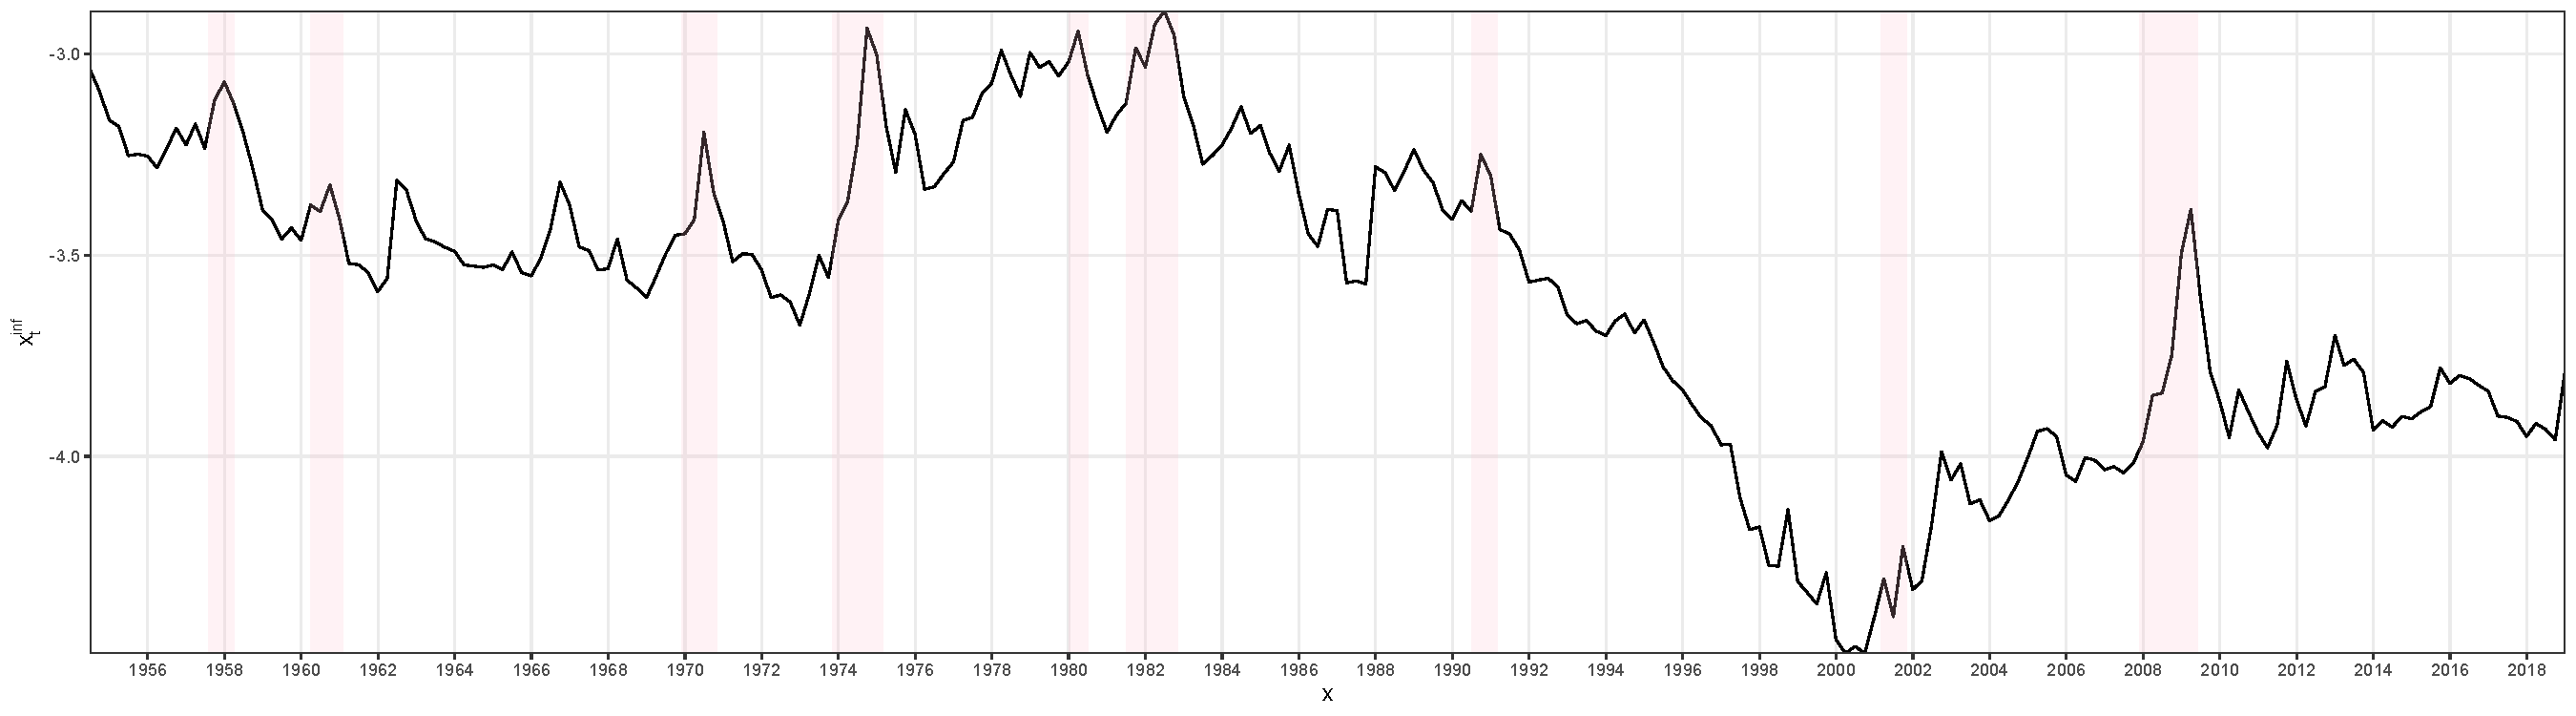
\includegraphics[width=1\linewidth]{Master_Thesis_Andreas_Kracht_Frandsen_files/figure-latex/DP-tids-1} 

}

\caption{Tidsserie af log Dividend Price Ratio.}\label{fig:DP-tids}
\end{figure}

\begin{figure}[H]

{\centering 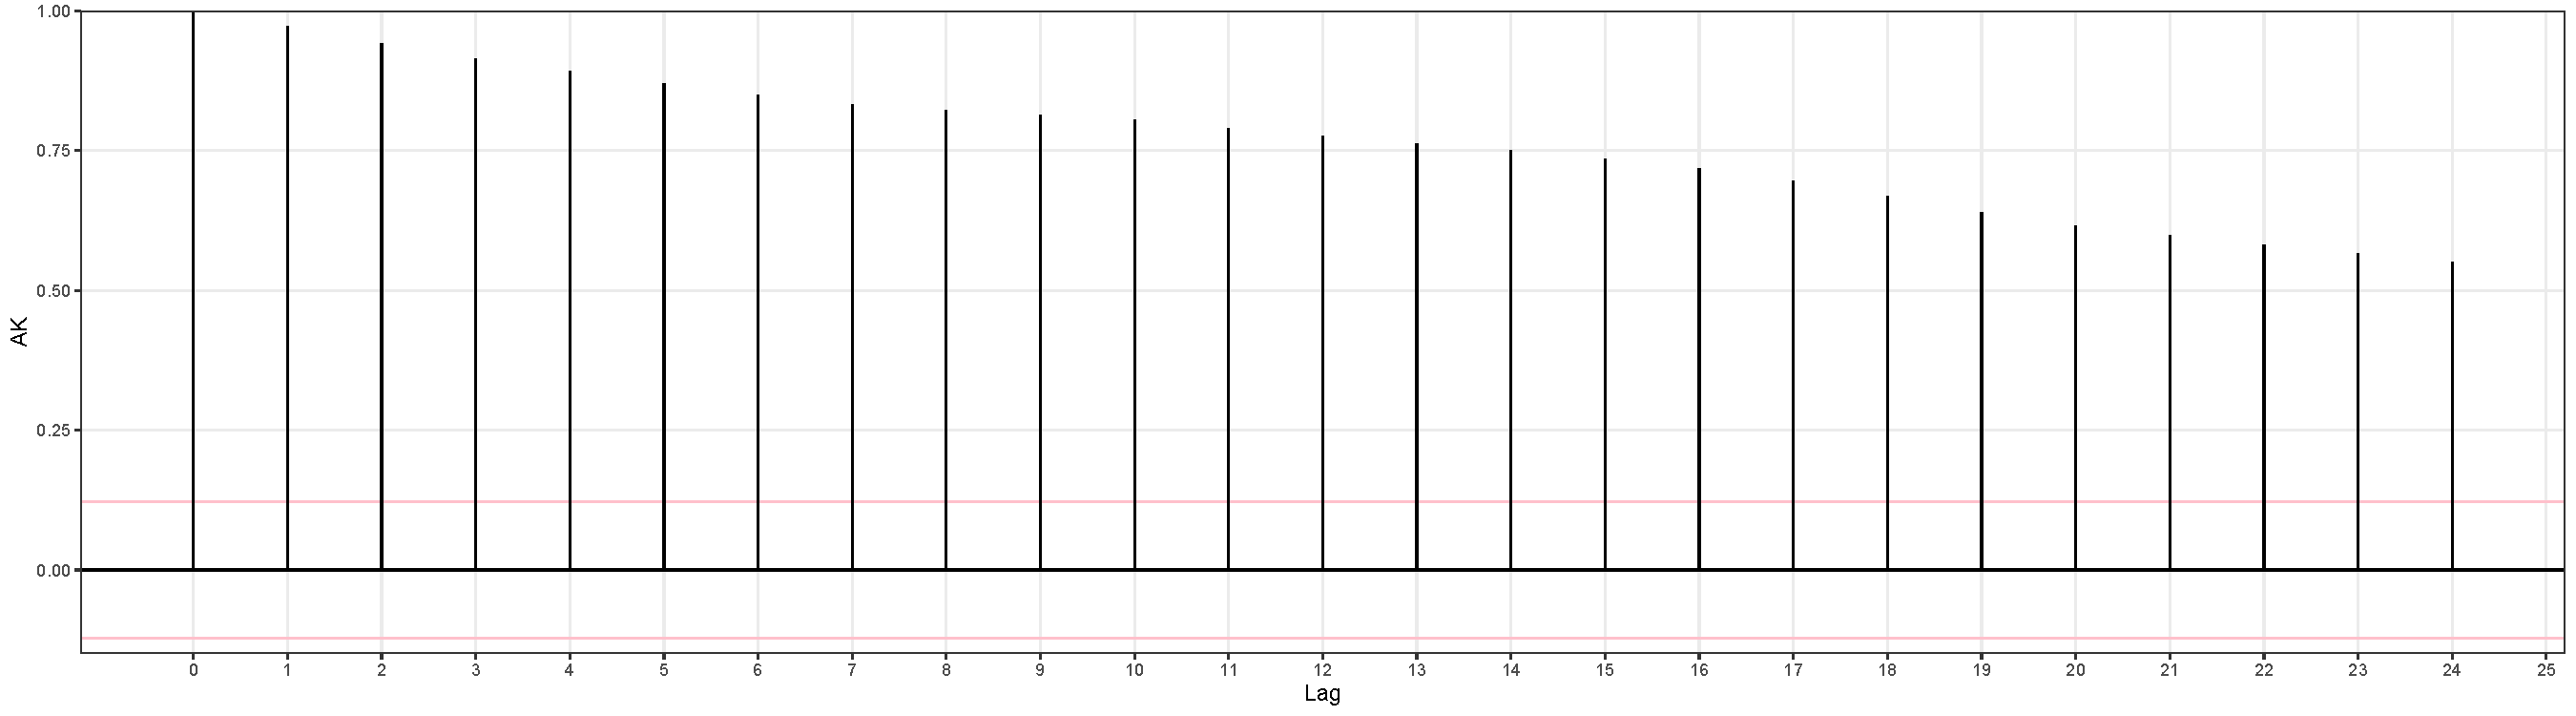
\includegraphics[width=1\linewidth]{Master_Thesis_Andreas_Kracht_Frandsen_files/figure-latex/DP-AK-1} 

}

\caption{Autokorrelation af log Dividend Price Ratio.}\label{fig:DP-AK}
\end{figure}

\begin{figure}[H]

{\centering 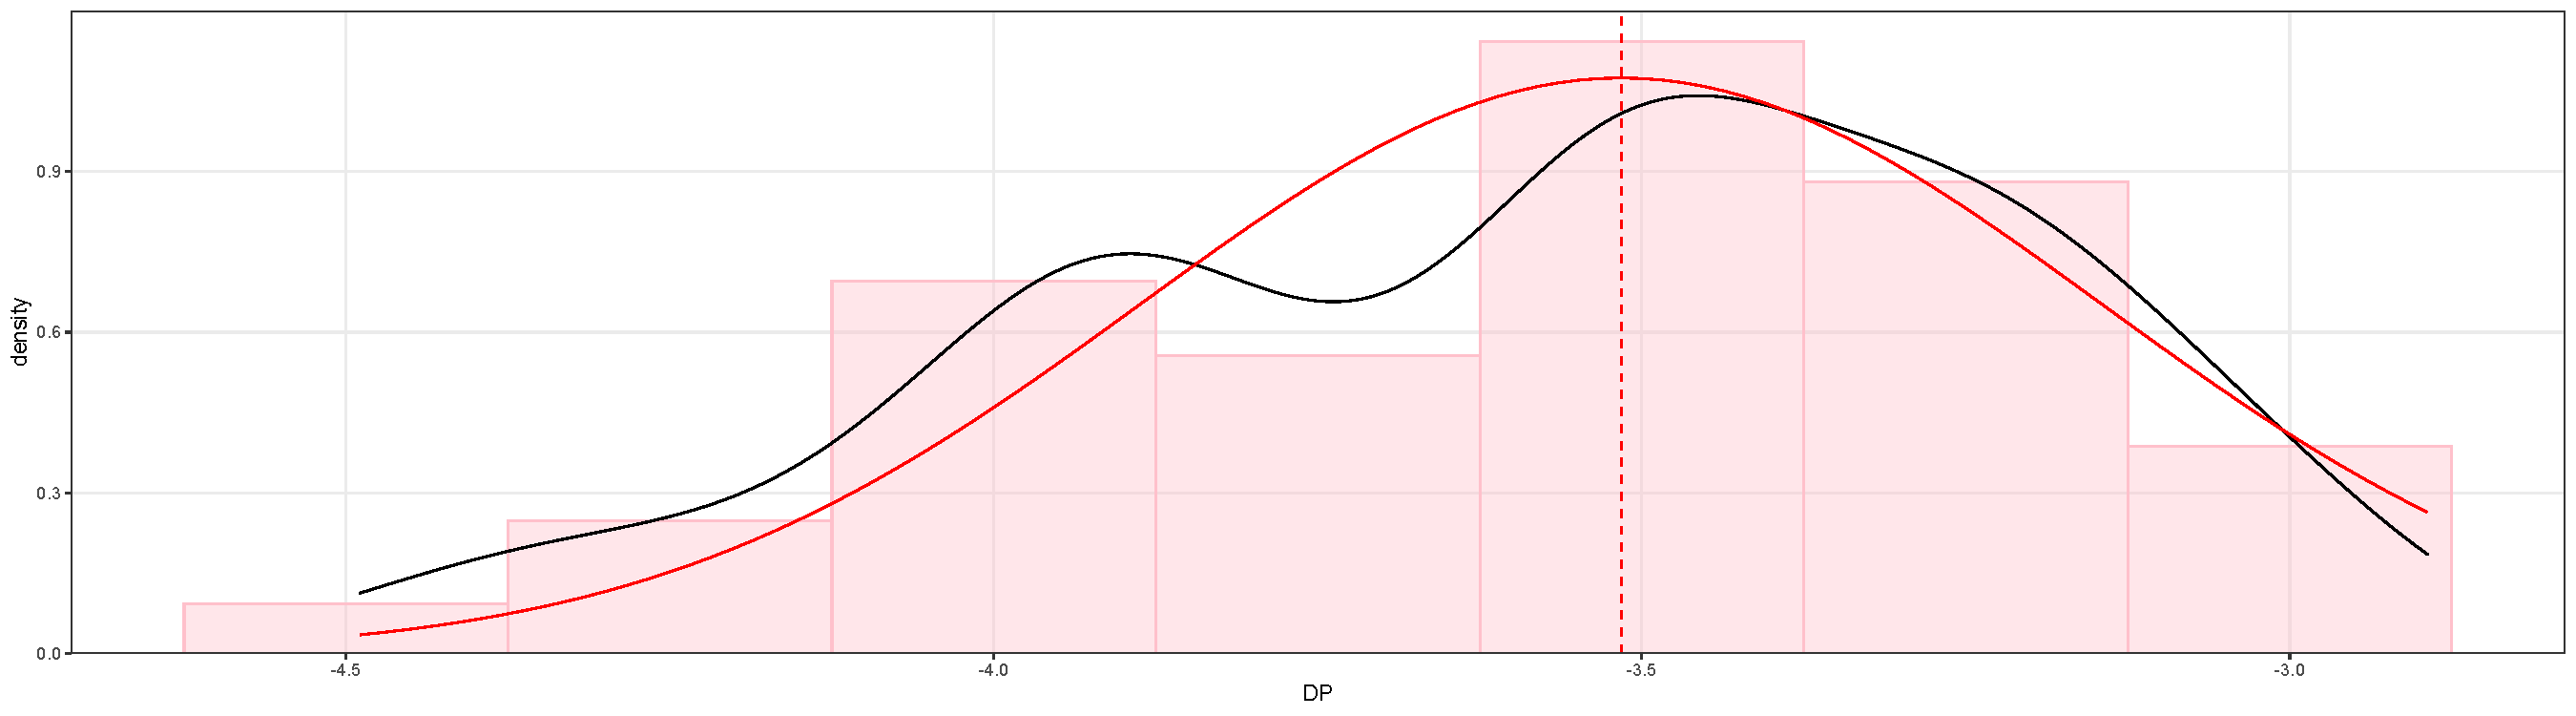
\includegraphics[width=1\linewidth]{Master_Thesis_Andreas_Kracht_Frandsen_files/figure-latex/DP-HIST-1} 

}

\caption{Histogram for log Dividend Price Ratio.}\label{fig:DP-HIST}
\end{figure}

\hypertarget{price-earnings-ratio-x_ttextpe}{%
\subsection{\texorpdfstring{Price-Earnings Ratio -- \(x_t^{\text{pe}}\)}{Price-Earnings Ratio -- x\_t\^{}\{\textbackslash text\{pe\}\}}}\label{price-earnings-ratio-x_ttextpe}}

Priserne for forholdet mellem priser og indtjening er som ovenstående indeksniveauet fra Sektion \ref{dataak}, ekslusiv udbytte. Indtjeningen er en rullende sum repræsenterende indtjeningen på \emph{S\&P 500} indekset. Data er dermed fra hhv. \citep{CRSPakt}, hentet gennem \citep{WRDSakt} og \citep{Shiller2020}, hentet gennem \citep{Goyal2007}. At indtjeningen benytter et andet datagrundlag end aktieindekset kan skabe tvetydigheder i resultaterne, men prædiktabiltetsegenskaben for variablen er stadig intakt. Log \emph{Price Earnings Ratio} bliver da beregnet som forskellen mellem de kvartalsvise log priser og de kvartalvise log indtjeninger. Den justerede middelværdi er 2.754\(\%\). Standardafvigelsen er på 0.407\(\%\). Derudover haves en højreskæv leptokurtisk fordeling med hhv. skævhed på 0.958 og kurtosis på 7.52. Figur \ref{fig:PE-tids} viser et plot over tidsserien, Figur \ref{fig:PE-AK} viser et plot over autokorrelationen for tidsserien og Figur \ref{fig:PE-HIST} viser et plot over histogrammet for tidsserien med tilhørende \emph{kernel} tæthed samt tæthed for en normalfordelt stokastisk variabel med middelværdi og standard afvigelse lig ovenstående estimater.

\begin{figure}[H]

{\centering 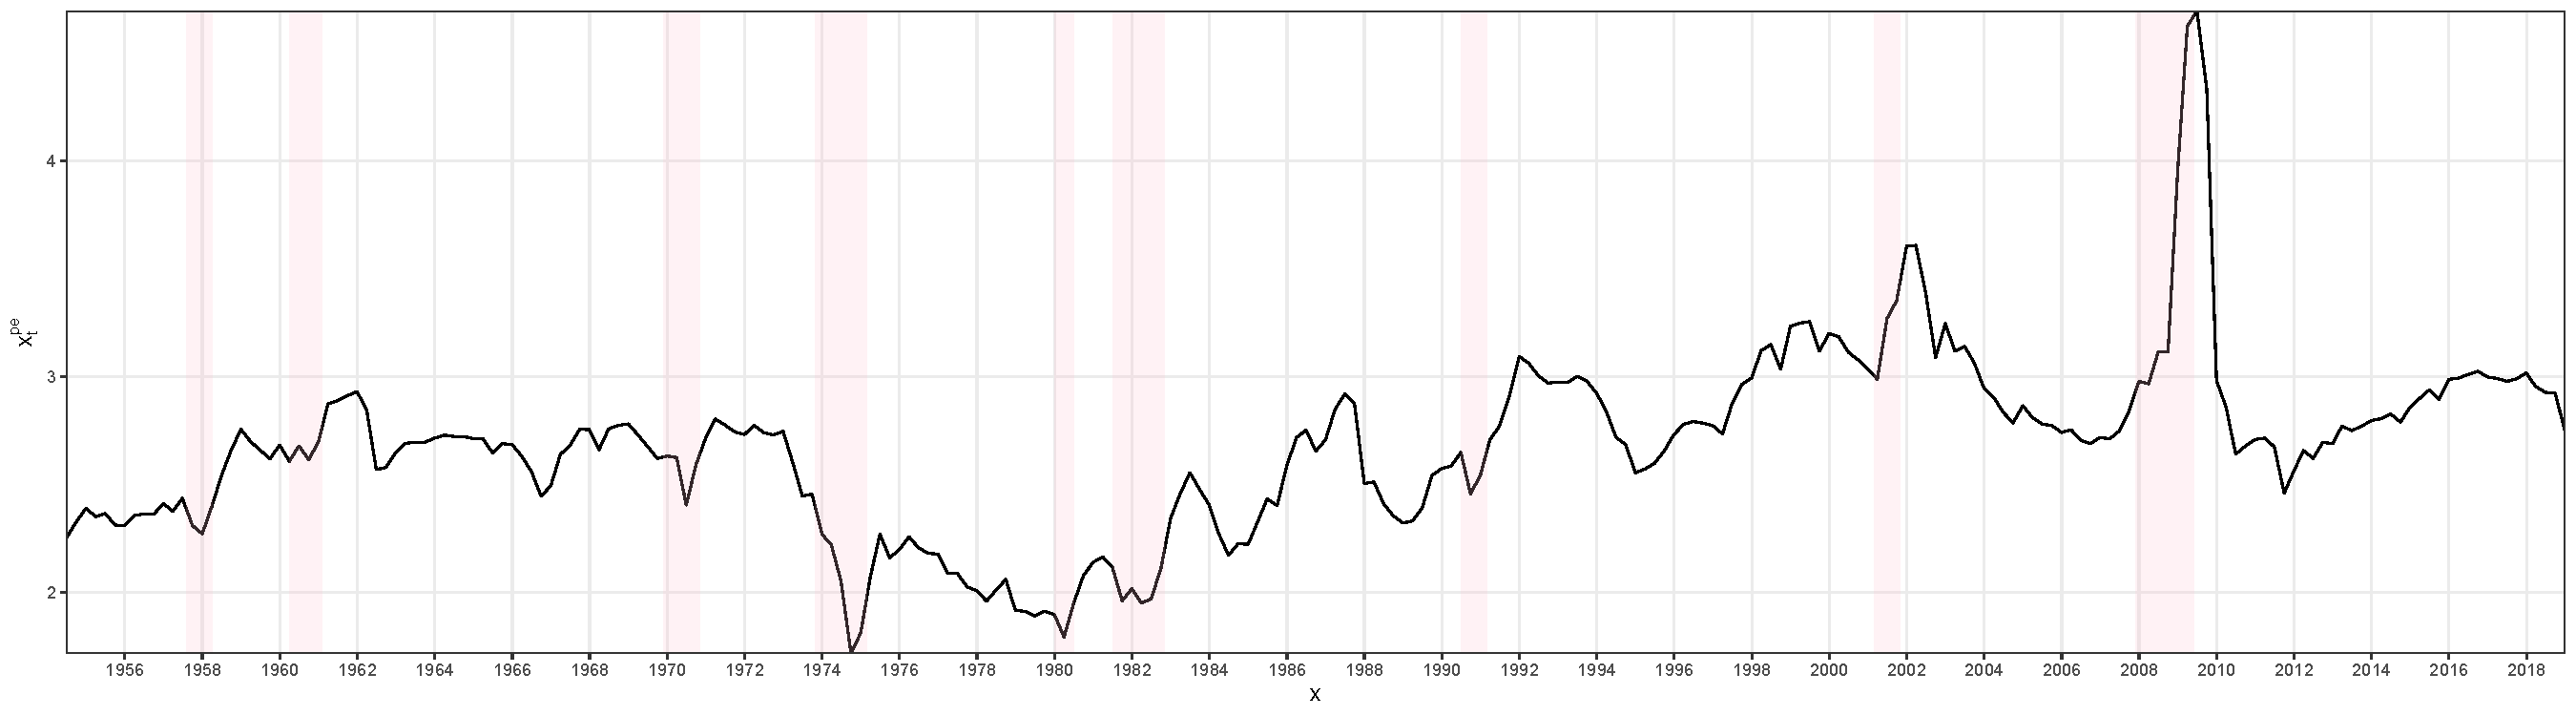
\includegraphics[width=1\linewidth]{Master_Thesis_Andreas_Kracht_Frandsen_files/figure-latex/PE-tids-1} 

}

\caption{Tidsserie af log Price Earnings Ratio.}\label{fig:PE-tids}
\end{figure}

\begin{figure}[H]

{\centering 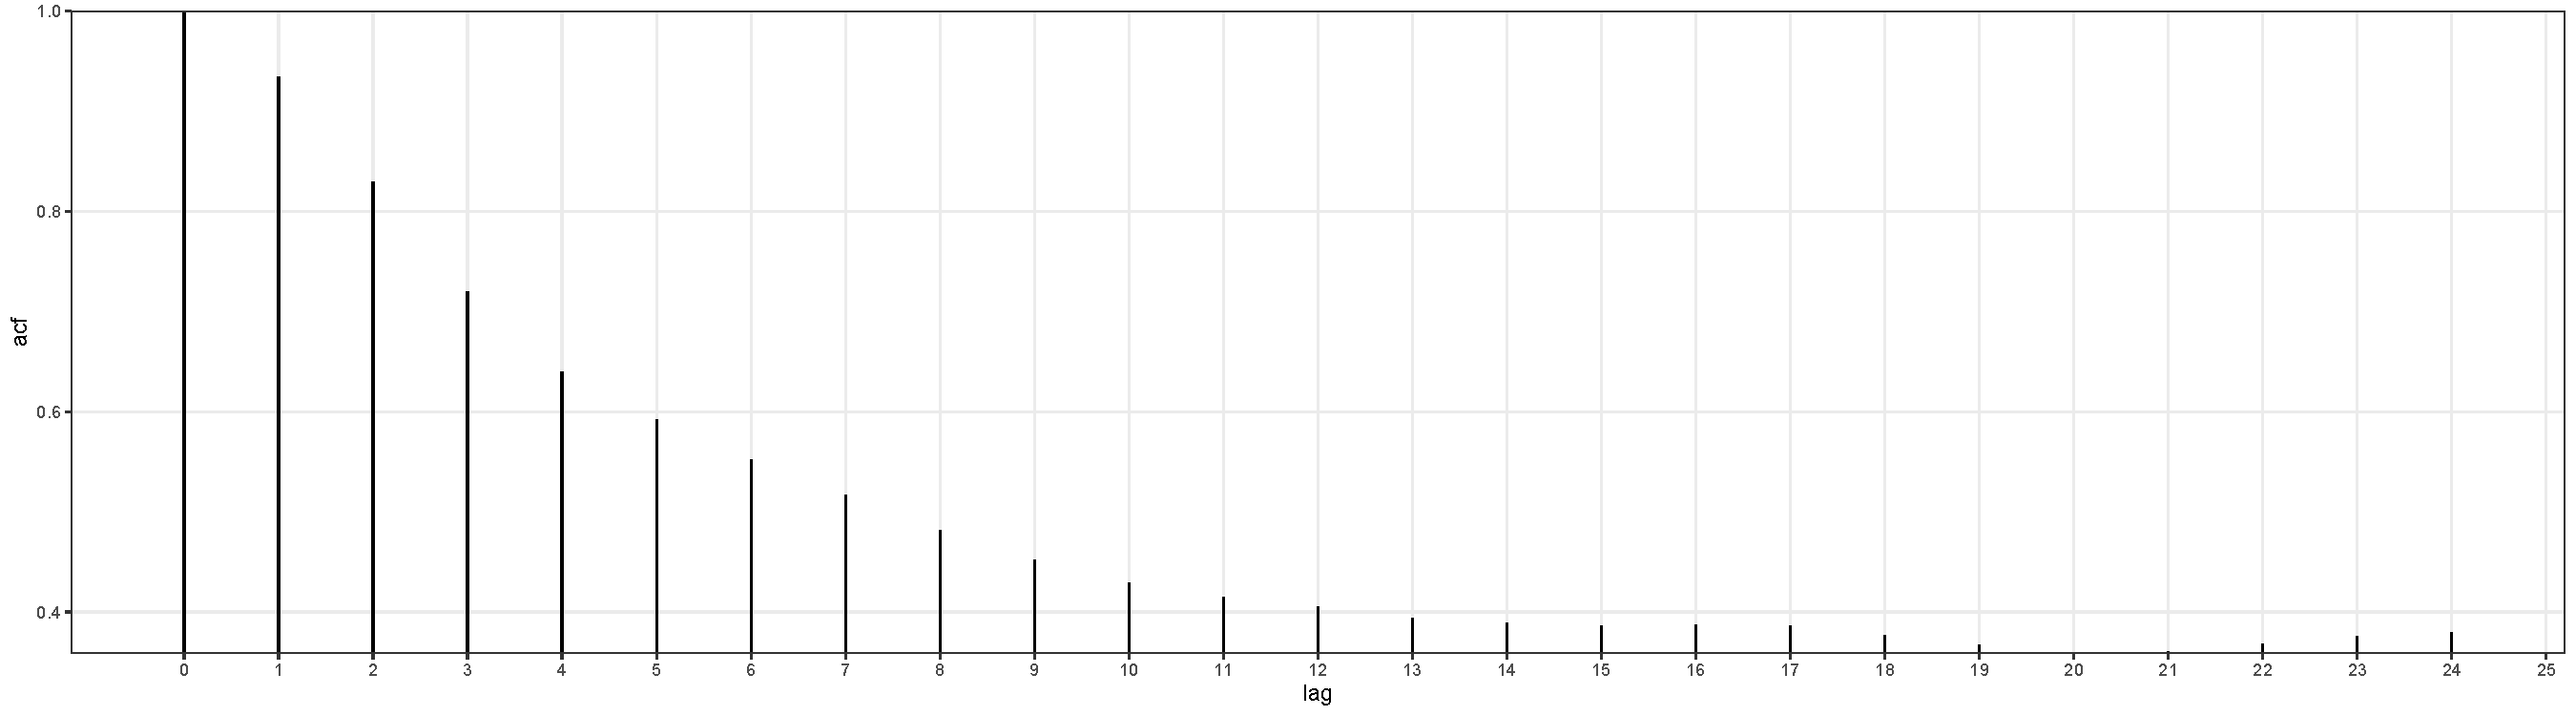
\includegraphics[width=1\linewidth]{Master_Thesis_Andreas_Kracht_Frandsen_files/figure-latex/PE-AK-1} 

}

\caption{Autokorrelation af log Price Earnings Ratio.}\label{fig:PE-AK}
\end{figure}

\begin{figure}[H]

{\centering 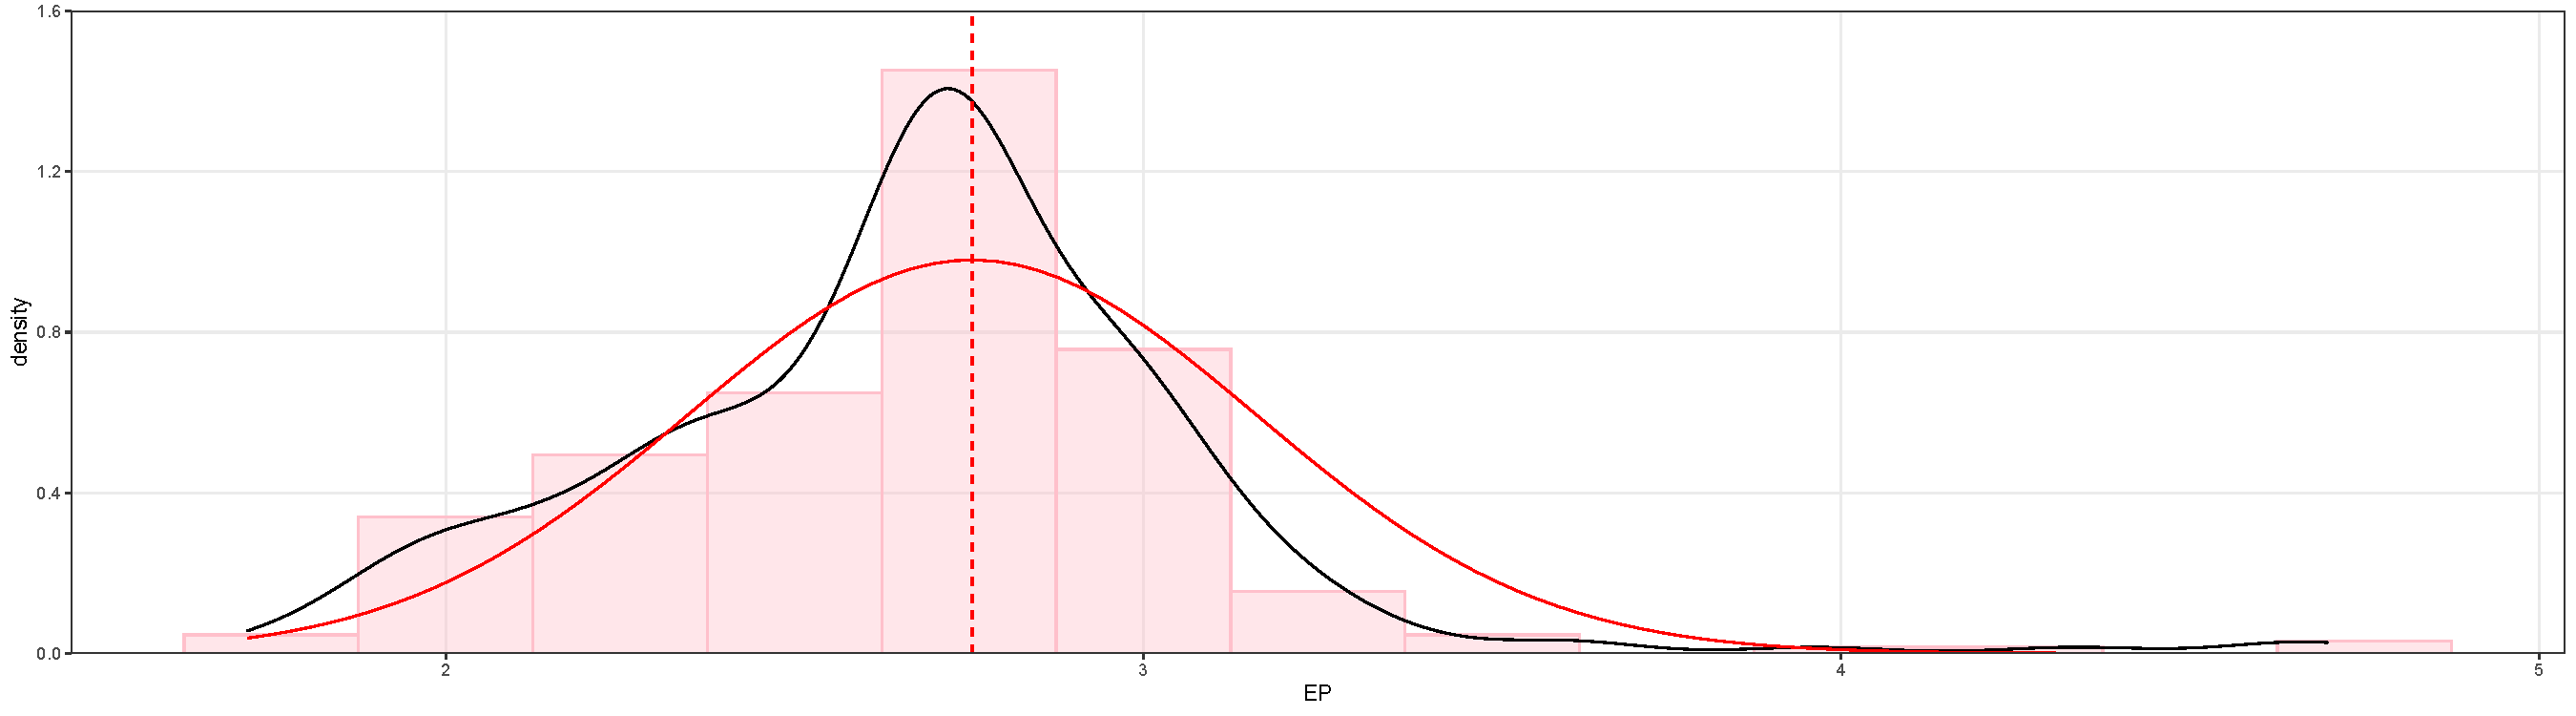
\includegraphics[width=1\linewidth]{Master_Thesis_Andreas_Kracht_Frandsen_files/figure-latex/PE-HIST-1} 

}

\caption{Histogram for log Price Earnings Ratio.}\label{fig:PE-HIST}
\end{figure}

\hypertarget{book-to-market-ratio-x_ttextbm}{%
\subsection{\texorpdfstring{Book-to-Market Ratio -- \(x_t^{\text{bm}}\)}{Book-to-Market Ratio -- x\_t\^{}\{\textbackslash text\{bm\}\}}}\label{book-to-market-ratio-x_ttextbm}}

\emph{Book-to-market Ratio} er hentet gennem \citep{Goyal2007}. Bogførte værdier samt markedsværdier stammer fra \emph{Value Line}'s hjemmeside, mere specifikt gennem deres \emph{Long-Term Perspective Chart} af indekset \emph{Dow Jones Industrial Average}. Beregningsmetoden er oprindeligt månedsbaseret og for månederne marts til december beregnes forholdet som den bogførte værdi fra slutningen af sidste år, delt med prisen fra seneste månedsultimo. For januar og februar beregnes det som den bogførte værdi fra slutningen af for to år siden, delt med prisen fra seneste månedsultimo. Beregningsmetoden er sammenlignelig med \citep{Kothari1997} og \citep{Pontiff1998}. Det første og andet moment er hhv. 0.505 og 0.248. Fra tredje og fjerde moment ses højreskævhed og en mesokurtisk fordeling. \citep{Pontiff1998} finder første og andet moment til hhv. \(0.505\) og \(0.252\), hvilket validerer estimaterne. Efter 1982 ses det, at forholdet aftager kraftigt, og efter en kort tiltagning har det de seneste år stabiliseret sig. Dette kommer sig bl.a. af, at amerikanske virksomheder i stigende grad har bogført en negativ værdi, se evt. \emph{Historical Book Equity Data} fra \citep{French2020}. Figur \ref{fig:BM-tids} viser et plot over tidsserien, Figur \ref{fig:BM-AK} viser et plot over autokorrelationen for tidsserien og Figur \ref{fig:BM-HIST} viser et plot over histogrammet for tidsserien med tilhørende \emph{kernel} tæthed samt tæthed for en normalfordelt stokastisk variabel med middelværdi og standard afvigelse lig ovenstående estimater.

\begin{figure}[H]

{\centering 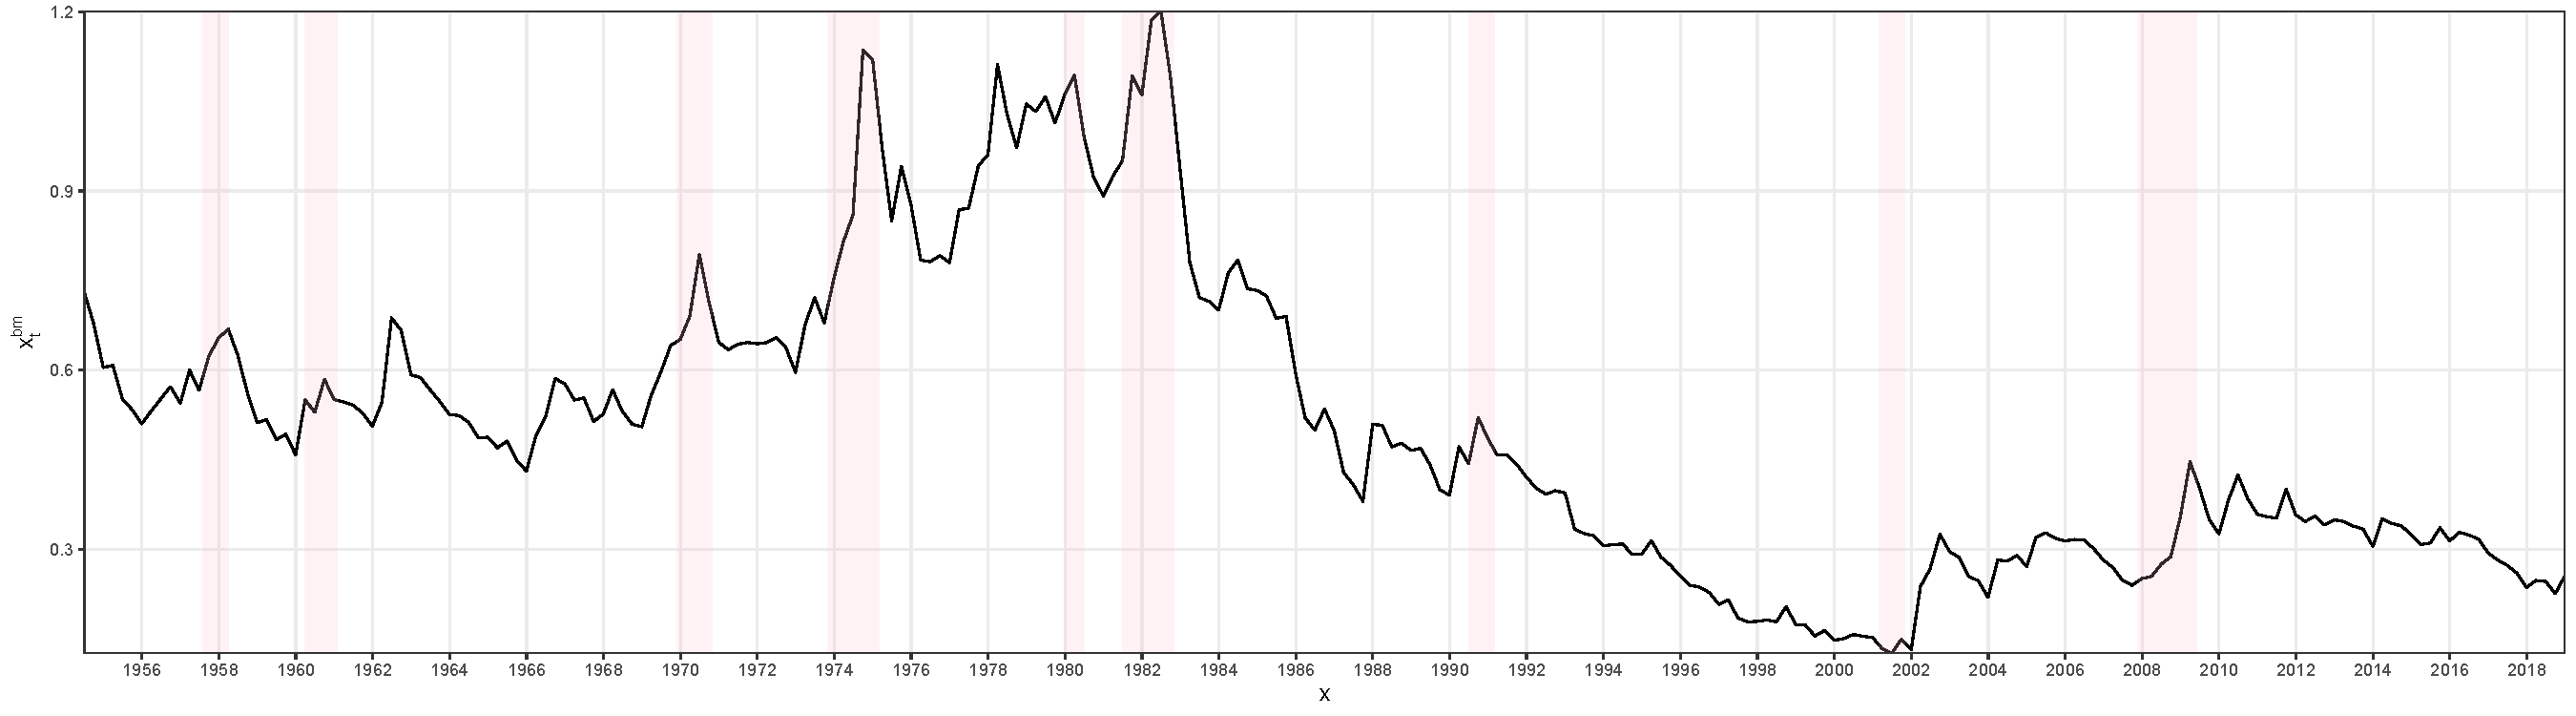
\includegraphics[width=1\linewidth]{Master_Thesis_Andreas_Kracht_Frandsen_files/figure-latex/BM-tids-1} 

}

\caption{Tidsserie af Book-to-market Ratio.}\label{fig:BM-tids}
\end{figure}

\begin{figure}[H]

{\centering 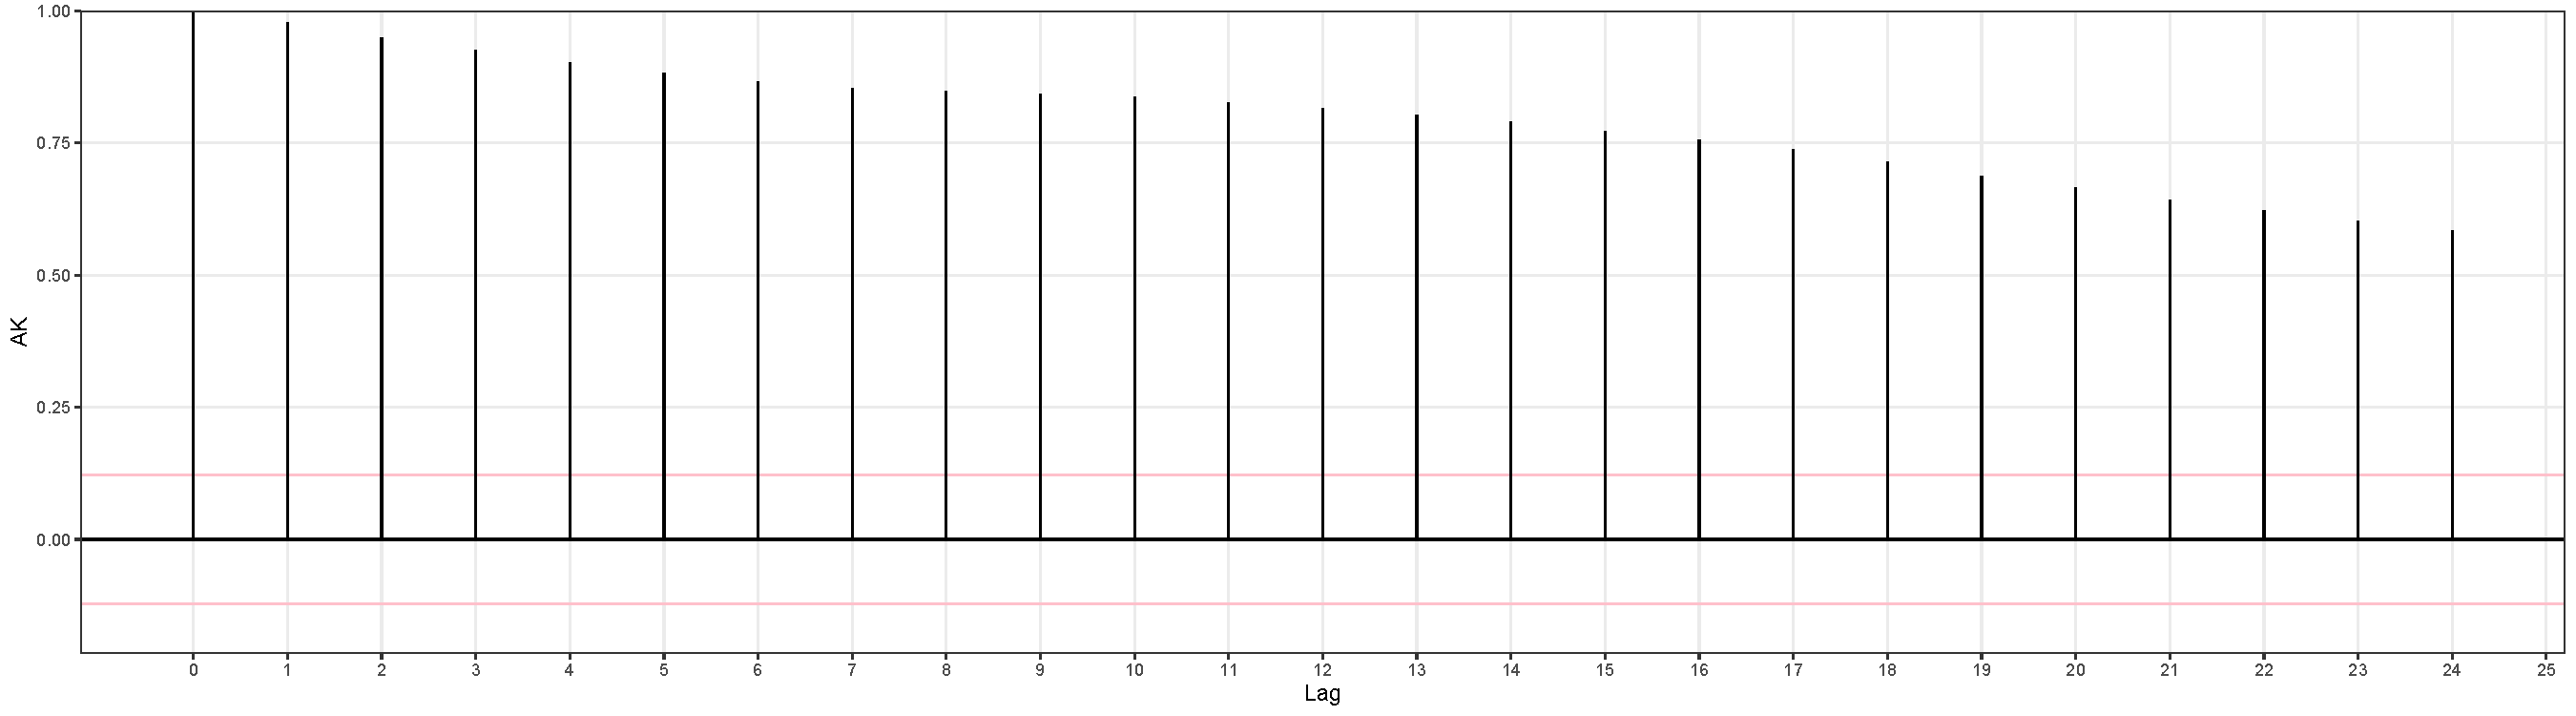
\includegraphics[width=1\linewidth]{Master_Thesis_Andreas_Kracht_Frandsen_files/figure-latex/BM-AK-1} 

}

\caption{Autokorrelation af Book-to-market Ratio.}\label{fig:BM-AK}
\end{figure}

\begin{figure}[H]

{\centering 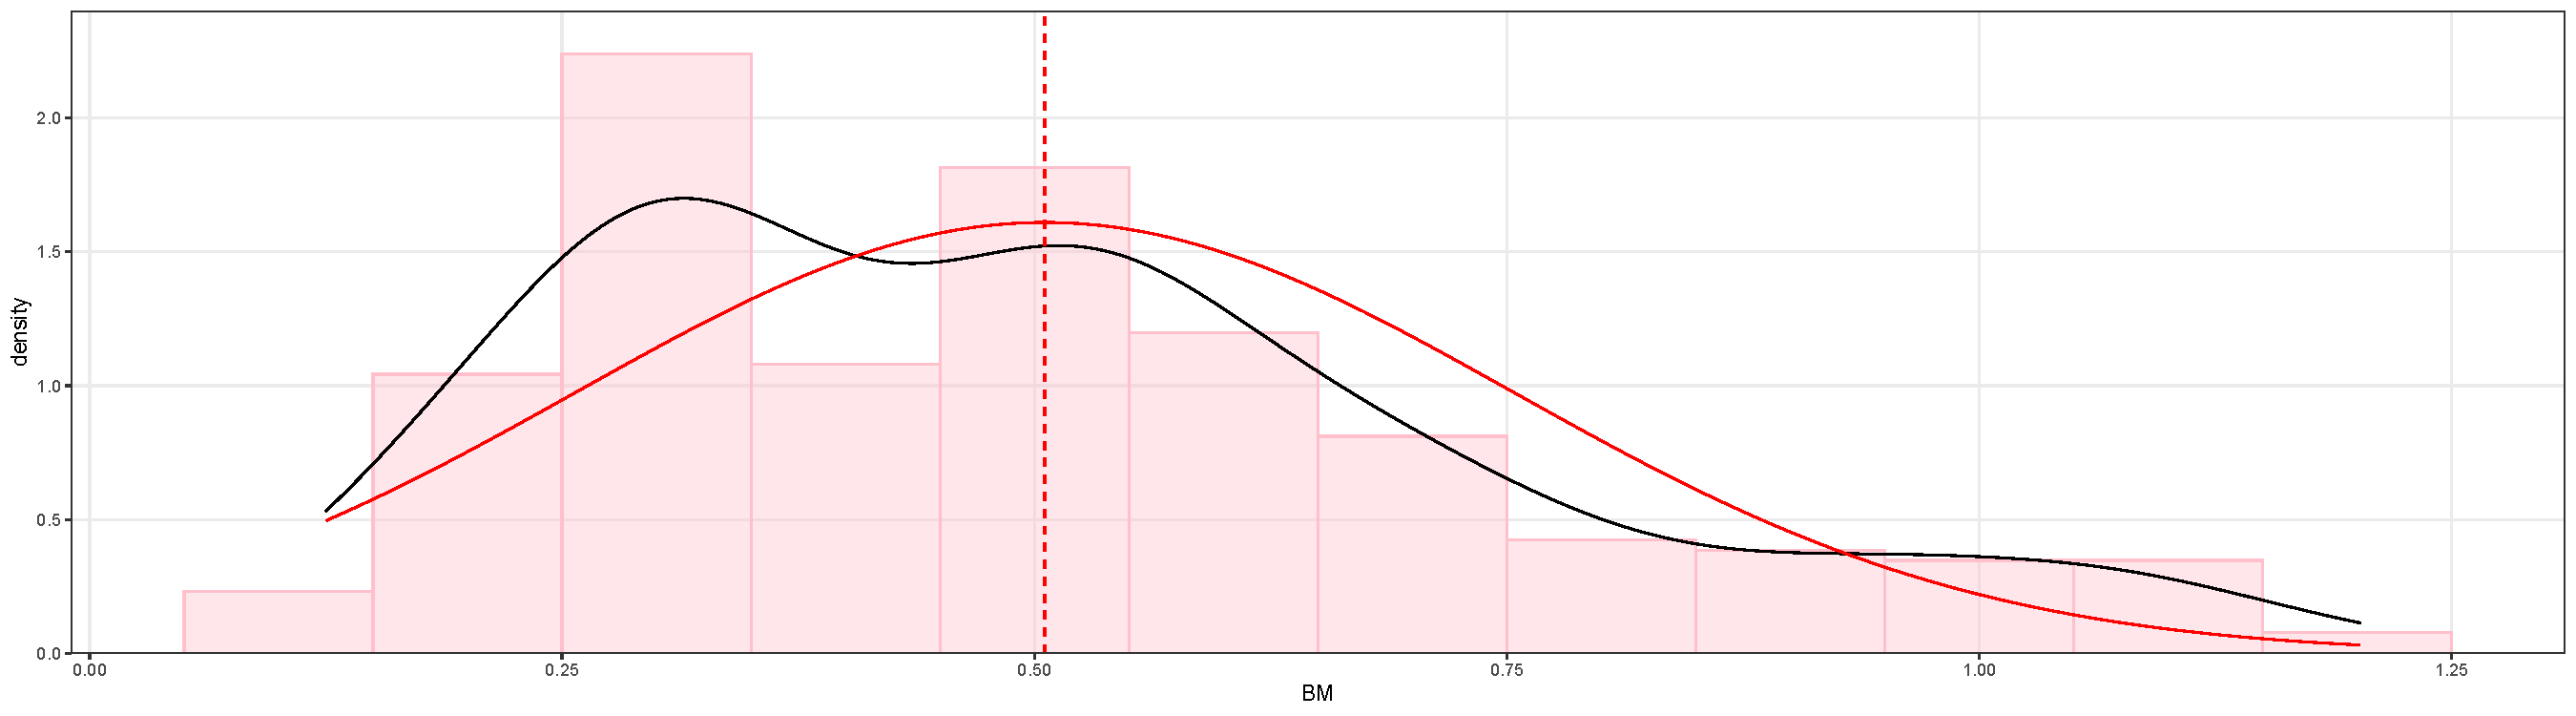
\includegraphics[width=1\linewidth]{Master_Thesis_Andreas_Kracht_Frandsen_files/figure-latex/BM-HIST-1} 

}

\caption{Histogram for Book-to-market Ratio.}\label{fig:BM-HIST}
\end{figure}

\hypertarget{aktievarians-x_ttextavar}{%
\subsection{\texorpdfstring{Aktievarians -- \(x_t^{\text{avar}}\)}{Aktievarians -- x\_t\^{}\{\textbackslash text\{avar\}\}}}\label{aktievarians-x_ttextavar}}

Aktievariansen består af den kvartalsvise kvadratsum af afkast, samt summen af produktet mellem to tilstødende kvartalsvise afkast. Beregningsmetoden er fra \citep{Schwert1987} og data er hentet gennem \citep{Goyal2007}, som baserer estimaterne på afkast fra \emph{S\&P 500} indekset. Selve metoden tager udgangspunkt i daglige priser fremfor kvartalsvise, for at måle det kvartalsvise aktieafkast \(r_{it}\). De kvartalsvise afkast er herefter kvadreret for at etablere variansen. Herefter justeres for autokorrelation, ved at addere to gange summen af produkterne mellem alle par af foreløbende kvartalsafkast. Middelværdien estimeres til 0.006 og med en standardafvigelse på 0.01. Givet ikke-negativiteten af variansen, ses forventeligt en meget højreskæv fordeling med tilhørende høj kurtosis på hhv. 7.186 og 68.38. Figur \ref{fig:AV-tids} viser et plot over tidsserien, Figur \ref{fig:AV-AK} viser et plot over autokorrelationen for tidsserien og Figur \ref{fig:AV-HIST} viser et plot over histogrammet for tidsserien med tilhørende \emph{kernel} tæthed samt tæthed for en normalfordelt stokastisk variabel med middelværdi og standard afvigelse lig ovenstående estimater.

\begin{figure}[H]

{\centering 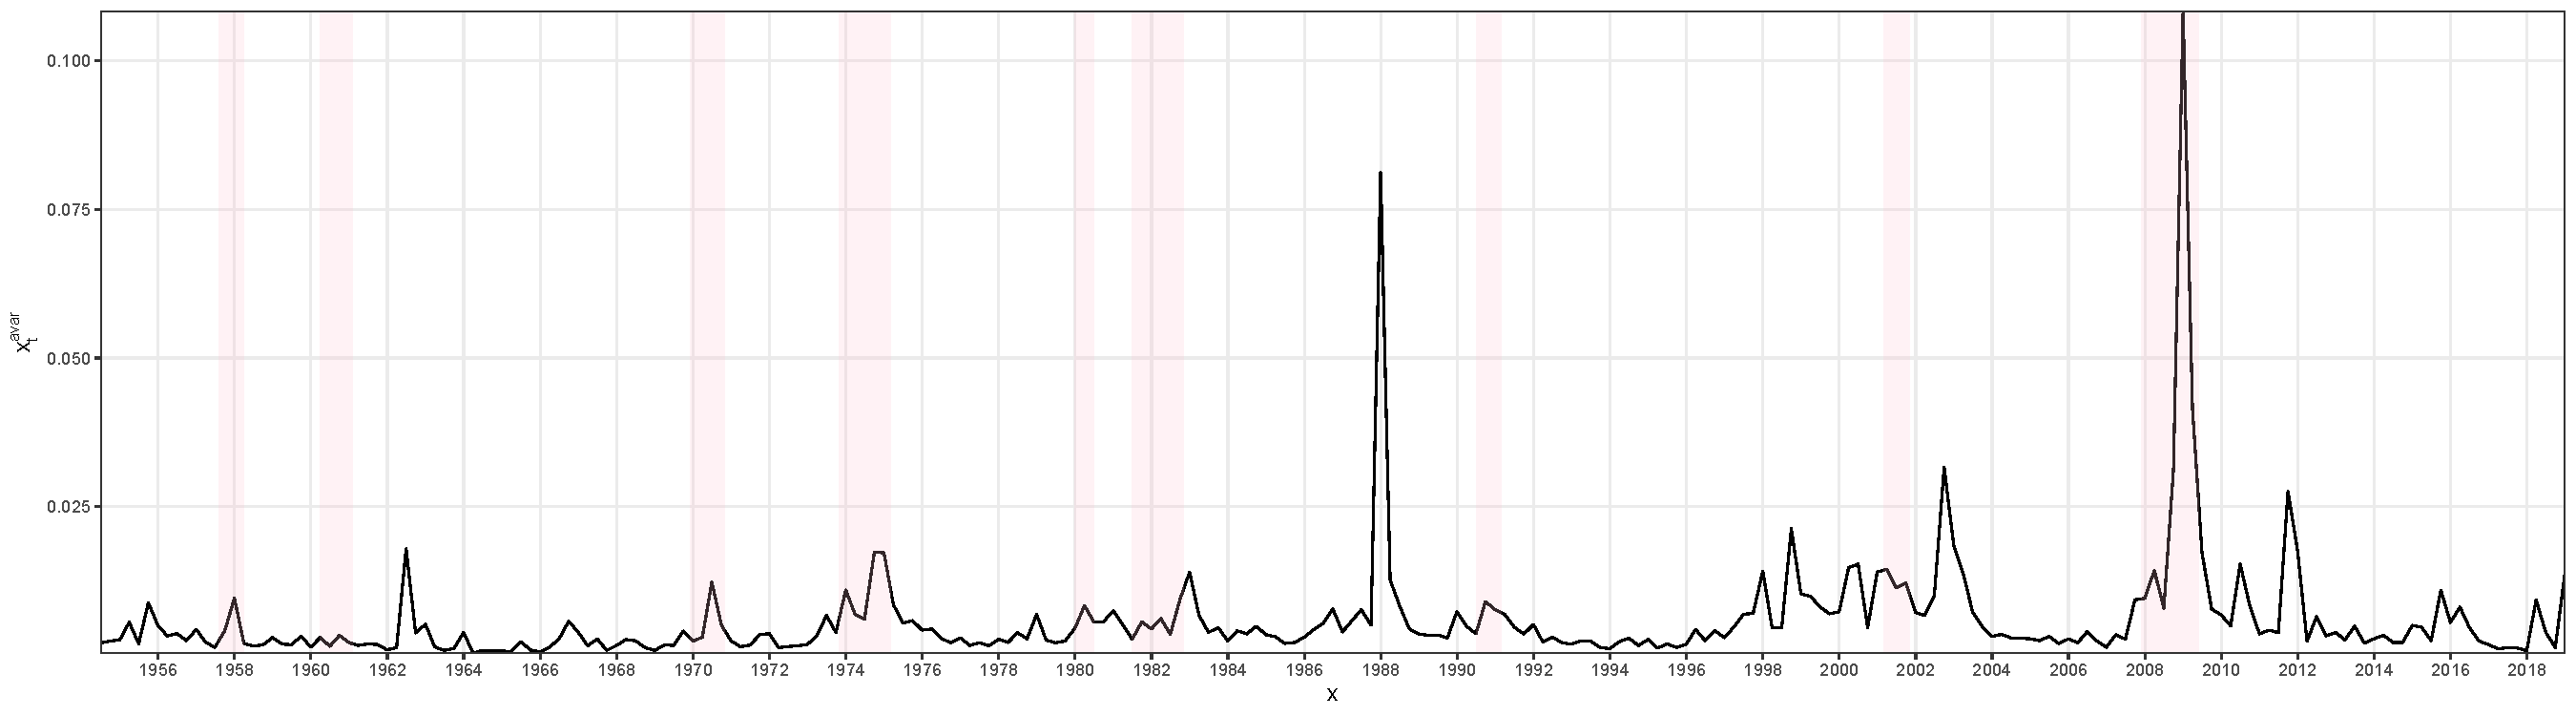
\includegraphics[width=1\linewidth]{Master_Thesis_Andreas_Kracht_Frandsen_files/figure-latex/AV-tids-1} 

}

\caption{Tidsserie af aktievariansen.}\label{fig:AV-tids}
\end{figure}

\begin{figure}[H]

{\centering 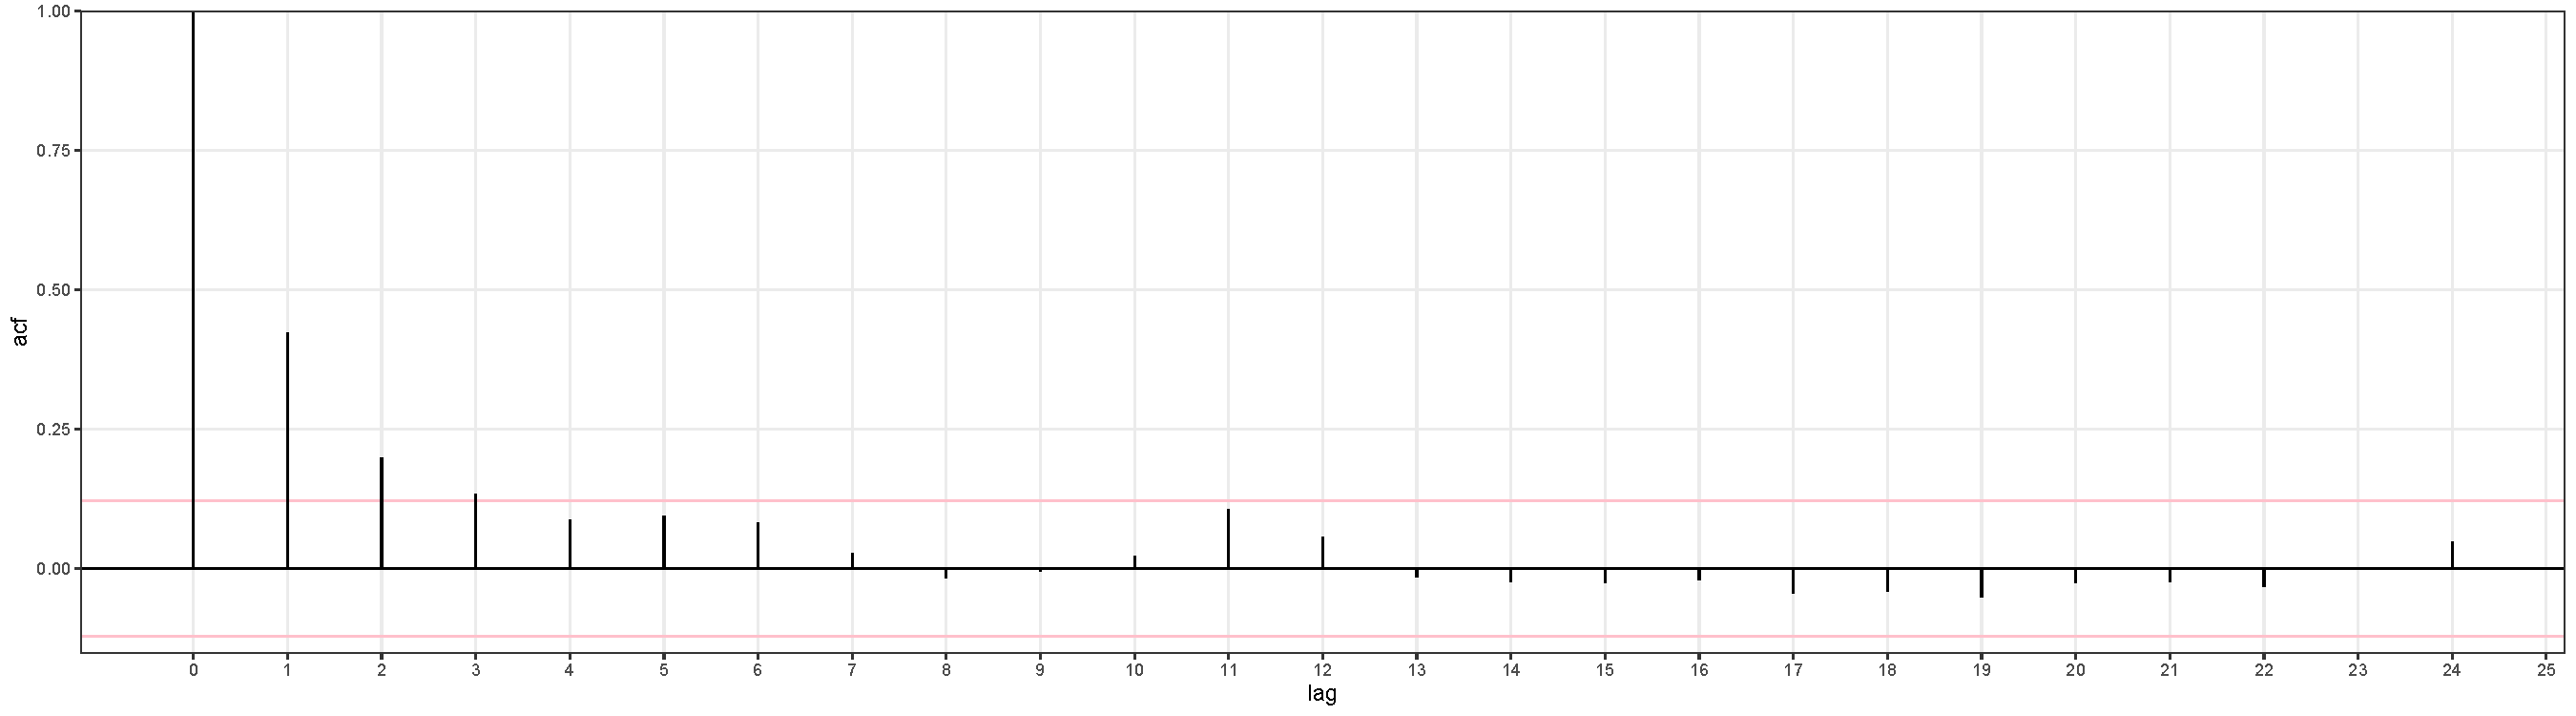
\includegraphics[width=1\linewidth]{Master_Thesis_Andreas_Kracht_Frandsen_files/figure-latex/AV-AK-1} 

}

\caption{Autokorrelation af aktievariansen.}\label{fig:AV-AK}
\end{figure}

\begin{figure}[H]

{\centering 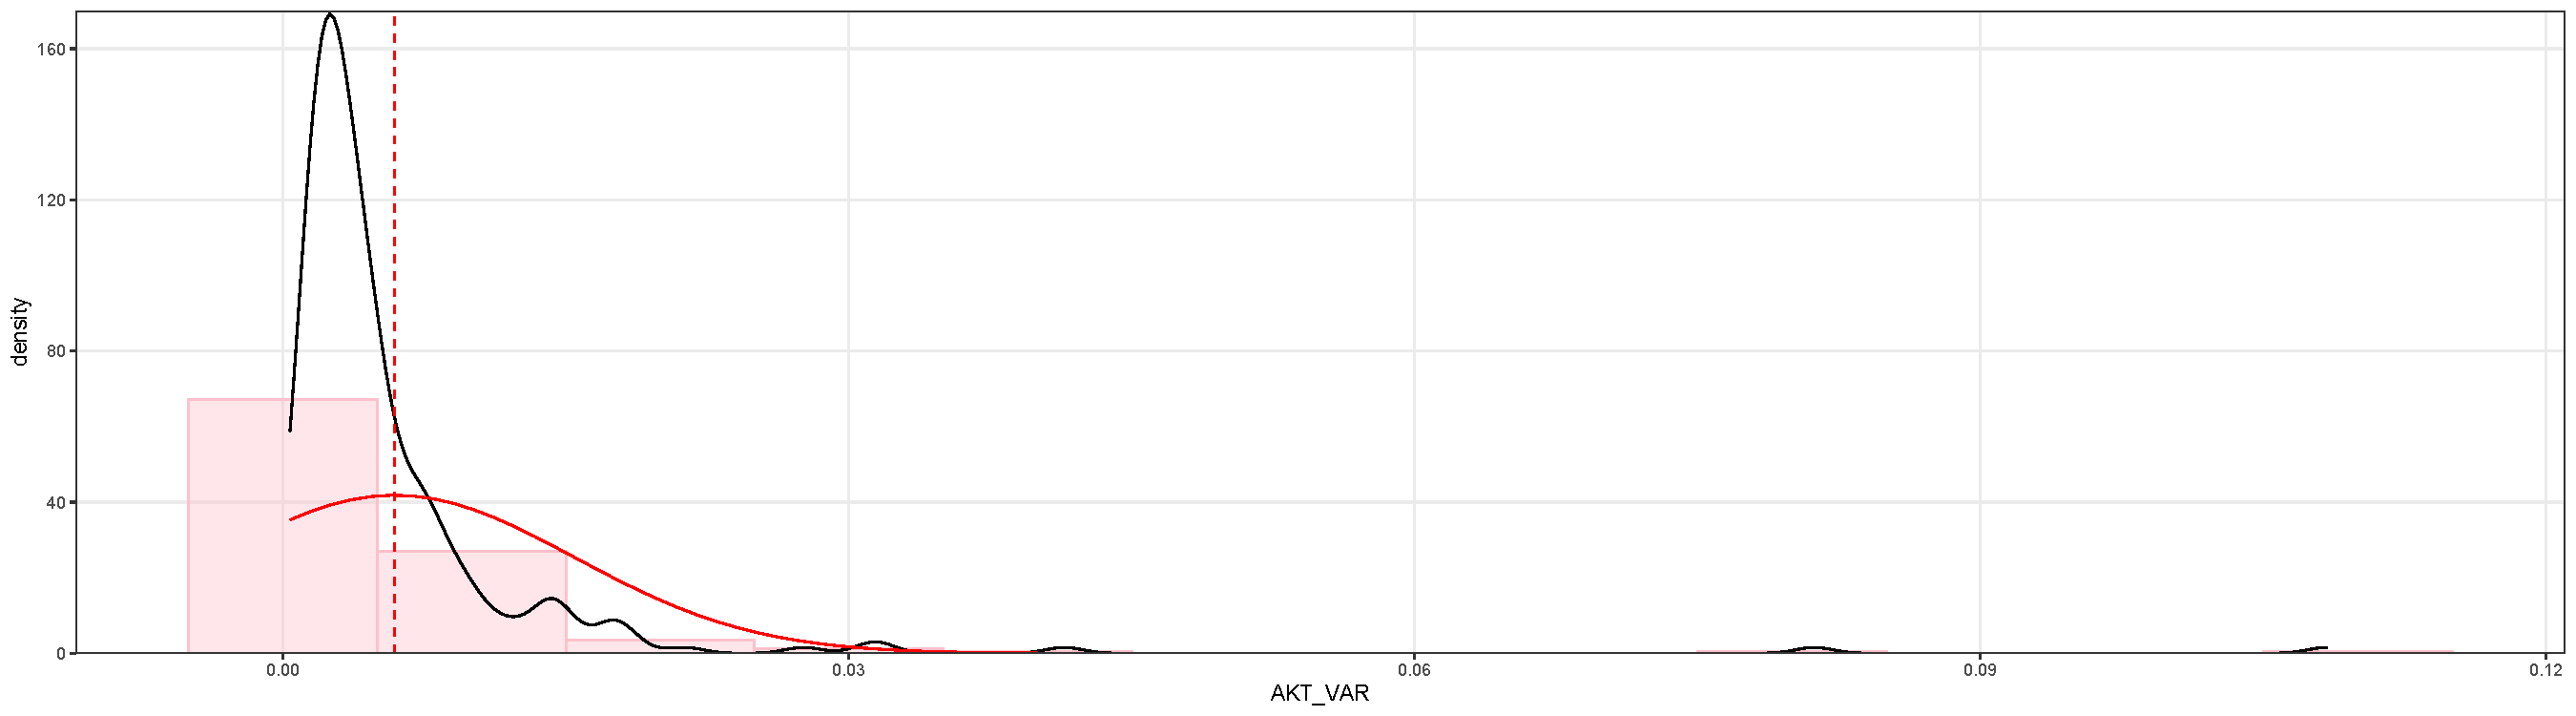
\includegraphics[width=1\linewidth]{Master_Thesis_Andreas_Kracht_Frandsen_files/figure-latex/AV-HIST-1} 

}

\caption{Histogram for aktievariansen.}\label{fig:AV-HIST}
\end{figure}

\hypertarget{datahml}{%
\subsection{\texorpdfstring{High Minus Low -- \(x_t^{\text{hml}}\)}{High Minus Low -- x\_t\^{}\{\textbackslash text\{hml\}\}}}\label{datahml}}

Den første af de to \emph{Fama-French} faktorer. Månedlige værdier er fra \citep{CRSPakt} og hentet gennem \citep{French2020}, det er herefter omdannet til kvartalsvise værdier via et kvartalsvist rullende tre-måneders gennemsnit. Selve faktoren er baseret på: to porteføljer baseret på størrelse, hvor skillelinjen er markedsmedianen på \emph{NYSE}, tre porteføljer baseret på \emph{Book-to-Market Ratio}, hvor skilningerne er \(30\)- og \(70\)-percentilerne af \emph{Book-to-Market Ratio} på \emph{NYSE}. Herefter eksisterer der seks fællesmængder, som dermed udgør grundlaget for porteføljerne til \emph{High Minus Low}. Selve faktoren beregnes som gennemsnittet på de to værdi-porteføljer\footnote{Virksomheder i værdi-porteføljerne har høj \emph{Book-to-market Ratio} og er hhv. store og små.} fratrukket det gennemsnitlige afkast på de to vækst-porteføljer\footnote{Virksomheder i vækst-porteføljerne har lav \emph{Book-to-market Ratio} og er hhv. store og små.}. En positiv \emph{High Minus Low} faktor medfører, at værdi-virksomheder er mere efficiente end vækst virksomheder på lang sigt, \citep{French1993}. Det første og andet moment er hhv. 0.33 og 1.809. Skævhed på 0.447 og kurtosis på 4.858, indikerer en forholdsvis symmetrisk fordeling. Figur \ref{fig:HML-tids} viser et plot over tidsserien, Figur \ref{fig:HML-AK} viser et plot over autokorrelationen for tidsserien og Figur \ref{fig:HML-HIST} viser et plot over histogrammet for tidsserien med tilhørende \emph{kernel} tæthed samt tæthed for en normalfordelt stokastisk variabel med middelværdi og standard afvigelse lig ovenstående estimater.

\begin{figure}[H]

{\centering 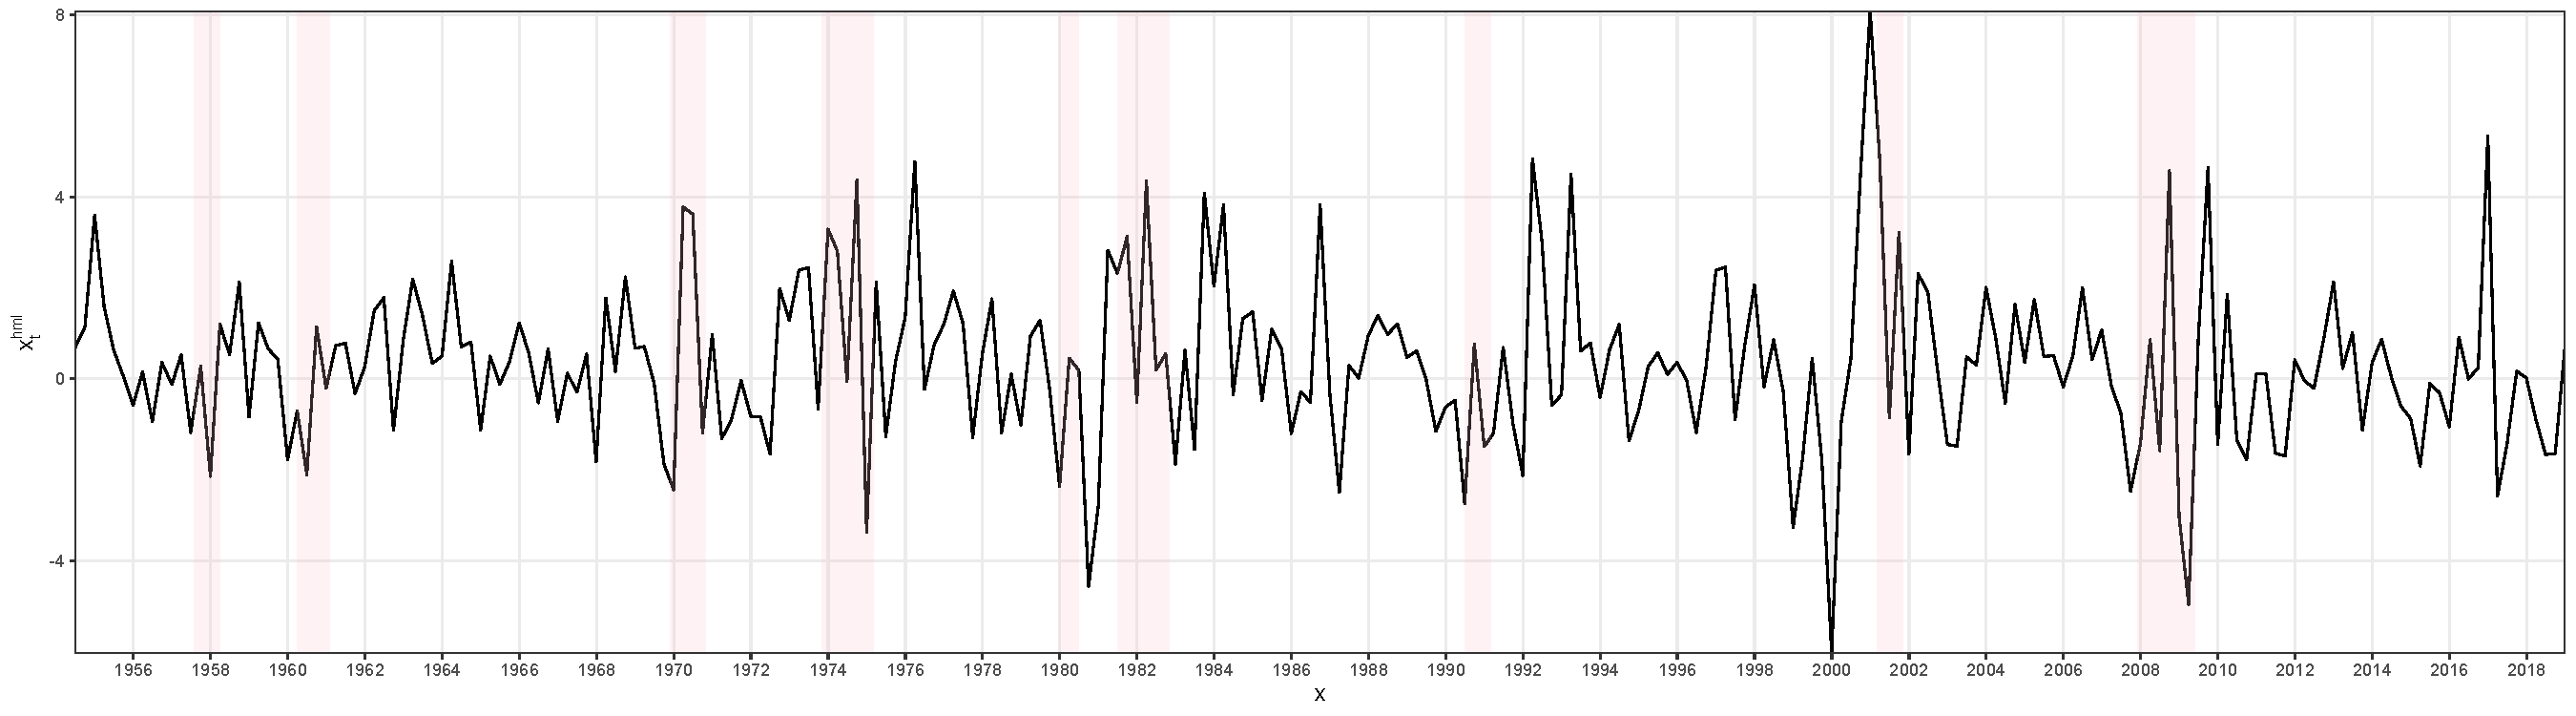
\includegraphics[width=1\linewidth]{Master_Thesis_Andreas_Kracht_Frandsen_files/figure-latex/HML-tids-1} 

}

\caption{Tidsserie af High Minus Low.}\label{fig:HML-tids}
\end{figure}

\begin{figure}[H]

{\centering 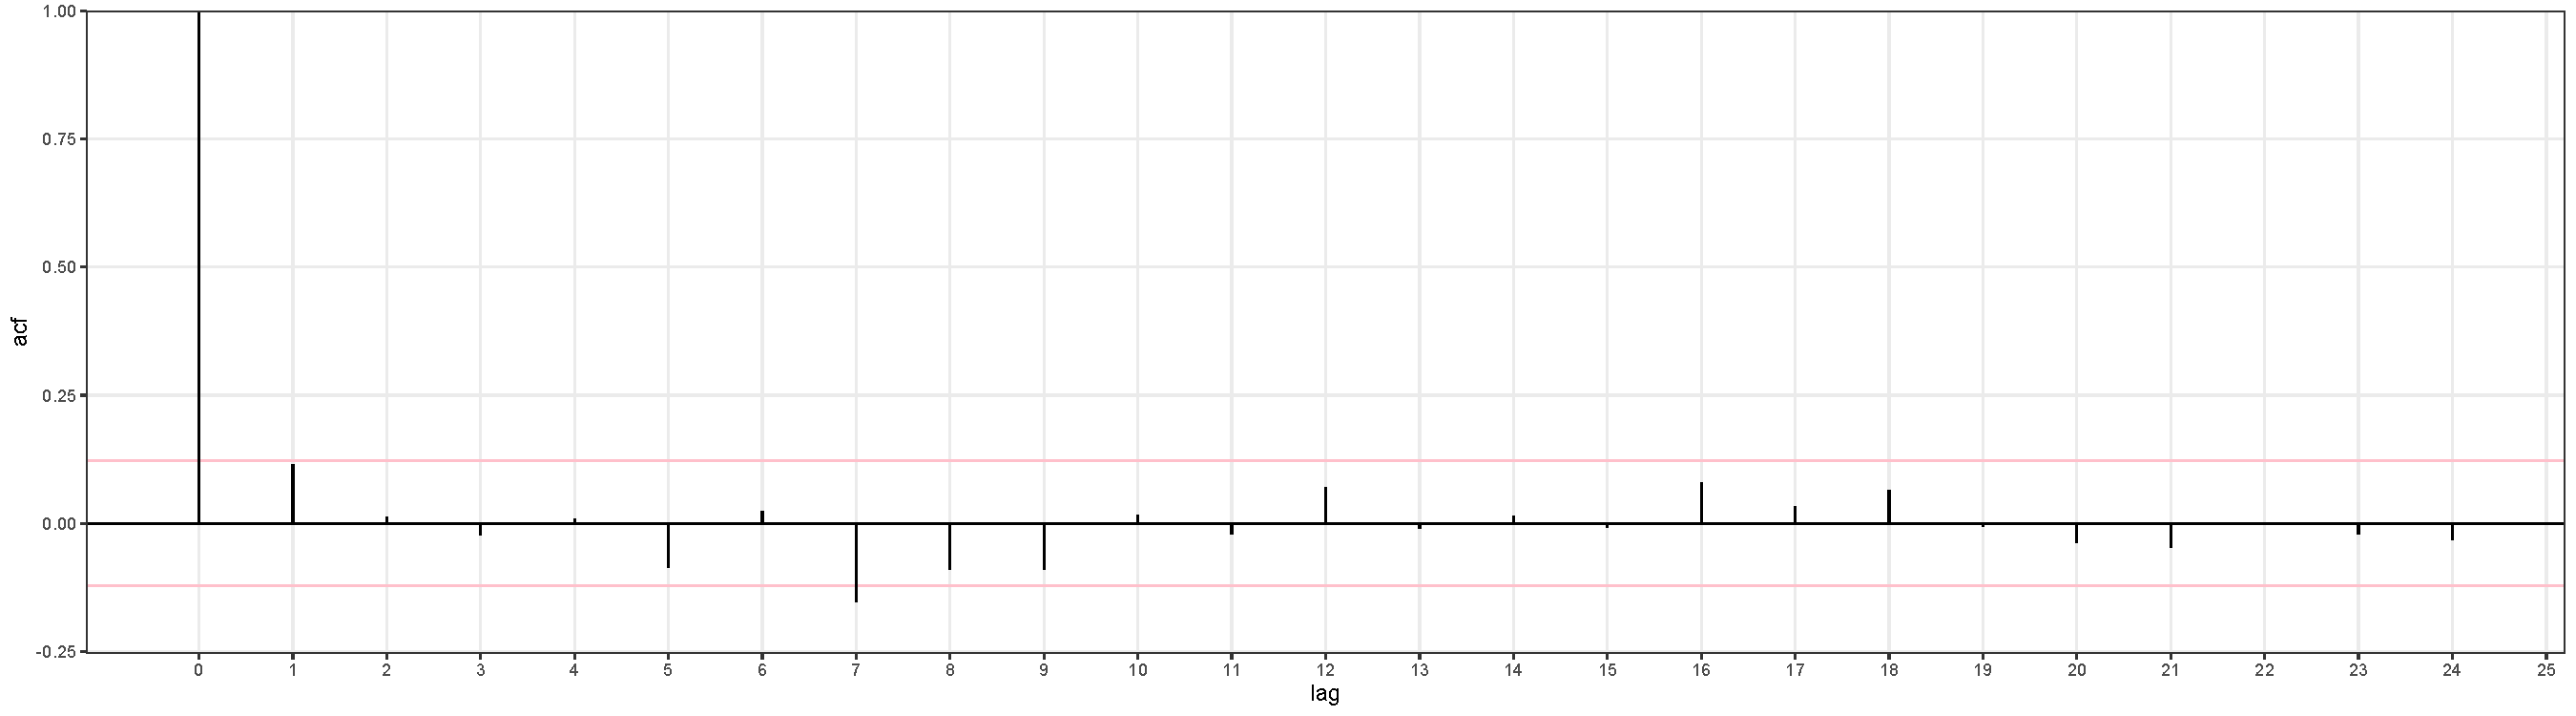
\includegraphics[width=1\linewidth]{Master_Thesis_Andreas_Kracht_Frandsen_files/figure-latex/HML-AK-1} 

}

\caption{Autokorrelation af High Minus Low.}\label{fig:HML-AK}
\end{figure}

\begin{figure}[H]

{\centering 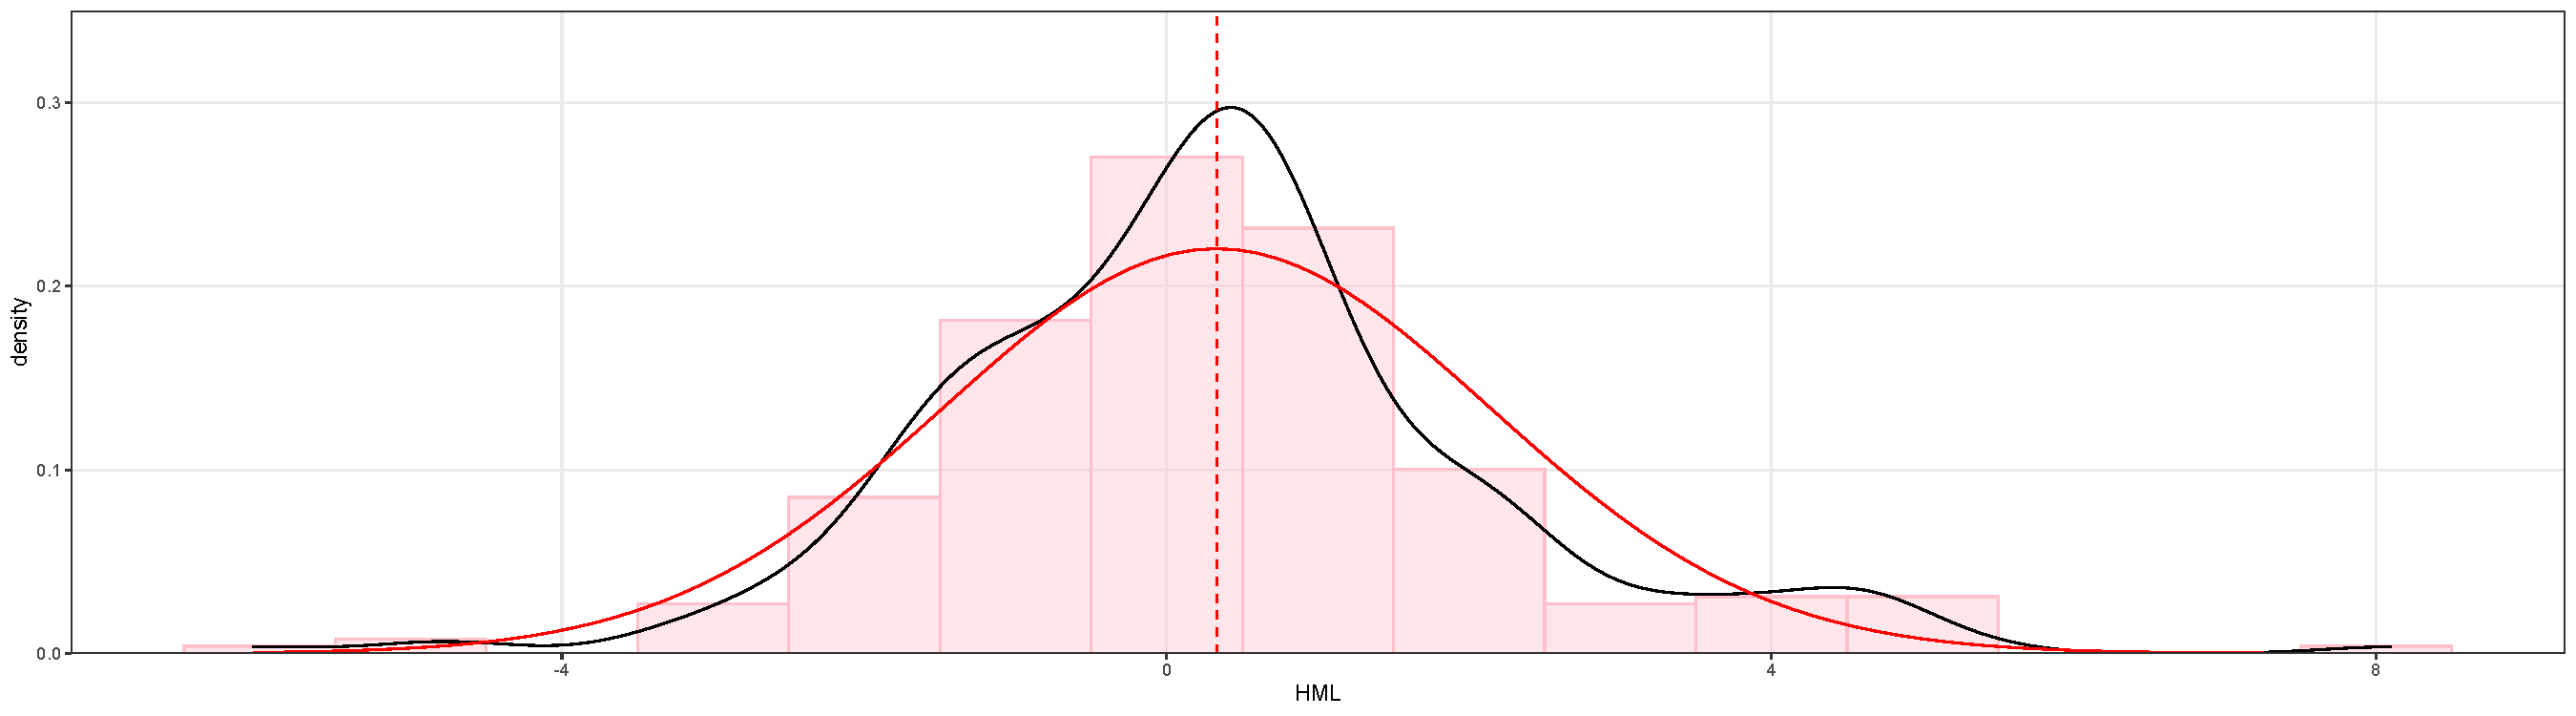
\includegraphics[width=1\linewidth]{Master_Thesis_Andreas_Kracht_Frandsen_files/figure-latex/HML-HIST-1} 

}

\caption{Histogram for High Minus Low.}\label{fig:HML-HIST}
\end{figure}

\hypertarget{datasmb}{%
\subsection{\texorpdfstring{Small Minus Big -- \(x_t^{\text{smb}}\)}{Small Minus Big -- x\_t\^{}\{\textbackslash text\{smb\}\}}}\label{datasmb}}

Den anden \emph{Fama-French} faktor. Månedlige værdier er fra \citep{CRSPakt} og hentet gennem \citep{French2020}, det er herefter omdannet til kvartalsvise værdier via et kvartalsvist rullende tre-måneders gennemsnit. Selve faktoren er baseret på de samme porteføljer som beskrevet i ovenstående Sektion \ref{datahml}. Selve faktoren beregnes som forskellen mellem de ligevægtede gennemsnitlige afkast af de små porteføljer og de store porteføljer. En positiv \emph{Small Minus Big} faktor er også kendt som \emph{Small Firm Effect}, og medfører, at små virksomheder er mere efficiente end store virksomheder på lang sigt, \citep{French1993}. Det første og andet moment er hhv. 0.168 og 1.717. En skævhed på 0.125 og kurtosis på 3.025, indikerer en meget symmetrisk fordeling. Figur \ref{fig:SMB-tids} viser et plot over tidsserien, Figur \ref{fig:SMB-AK} viser et plot over autokorrelationen for tidsserien og Figur \ref{fig:SMB-HIST} viser et plot over histogrammet for tidsserien med tilhørende \emph{kernel} tæthed samt tæthed for en normalfordelt stokastisk variabel med middelværdi og standard afvigelse lig ovenstående estimater.

\begin{figure}[H]

{\centering 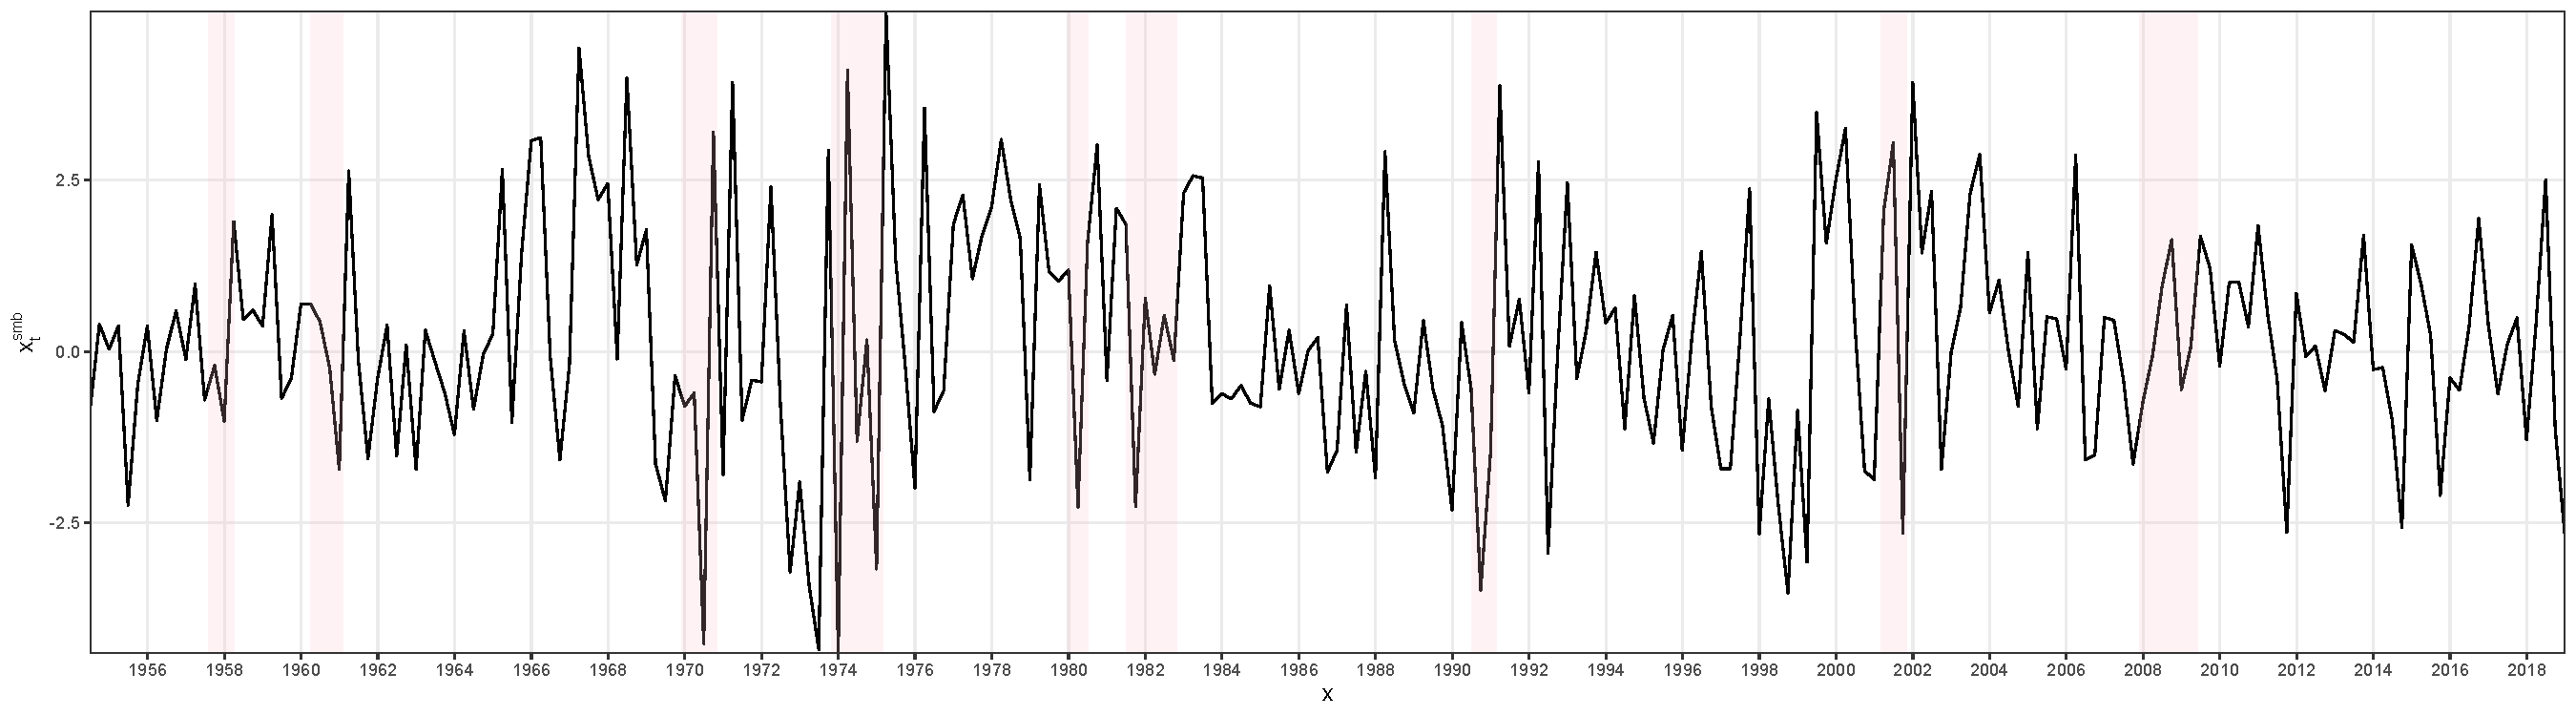
\includegraphics[width=1\linewidth]{Master_Thesis_Andreas_Kracht_Frandsen_files/figure-latex/SMB-tids-1} 

}

\caption{Tidsserie af Small Minus Big.}\label{fig:SMB-tids}
\end{figure}

\begin{figure}[H]

{\centering 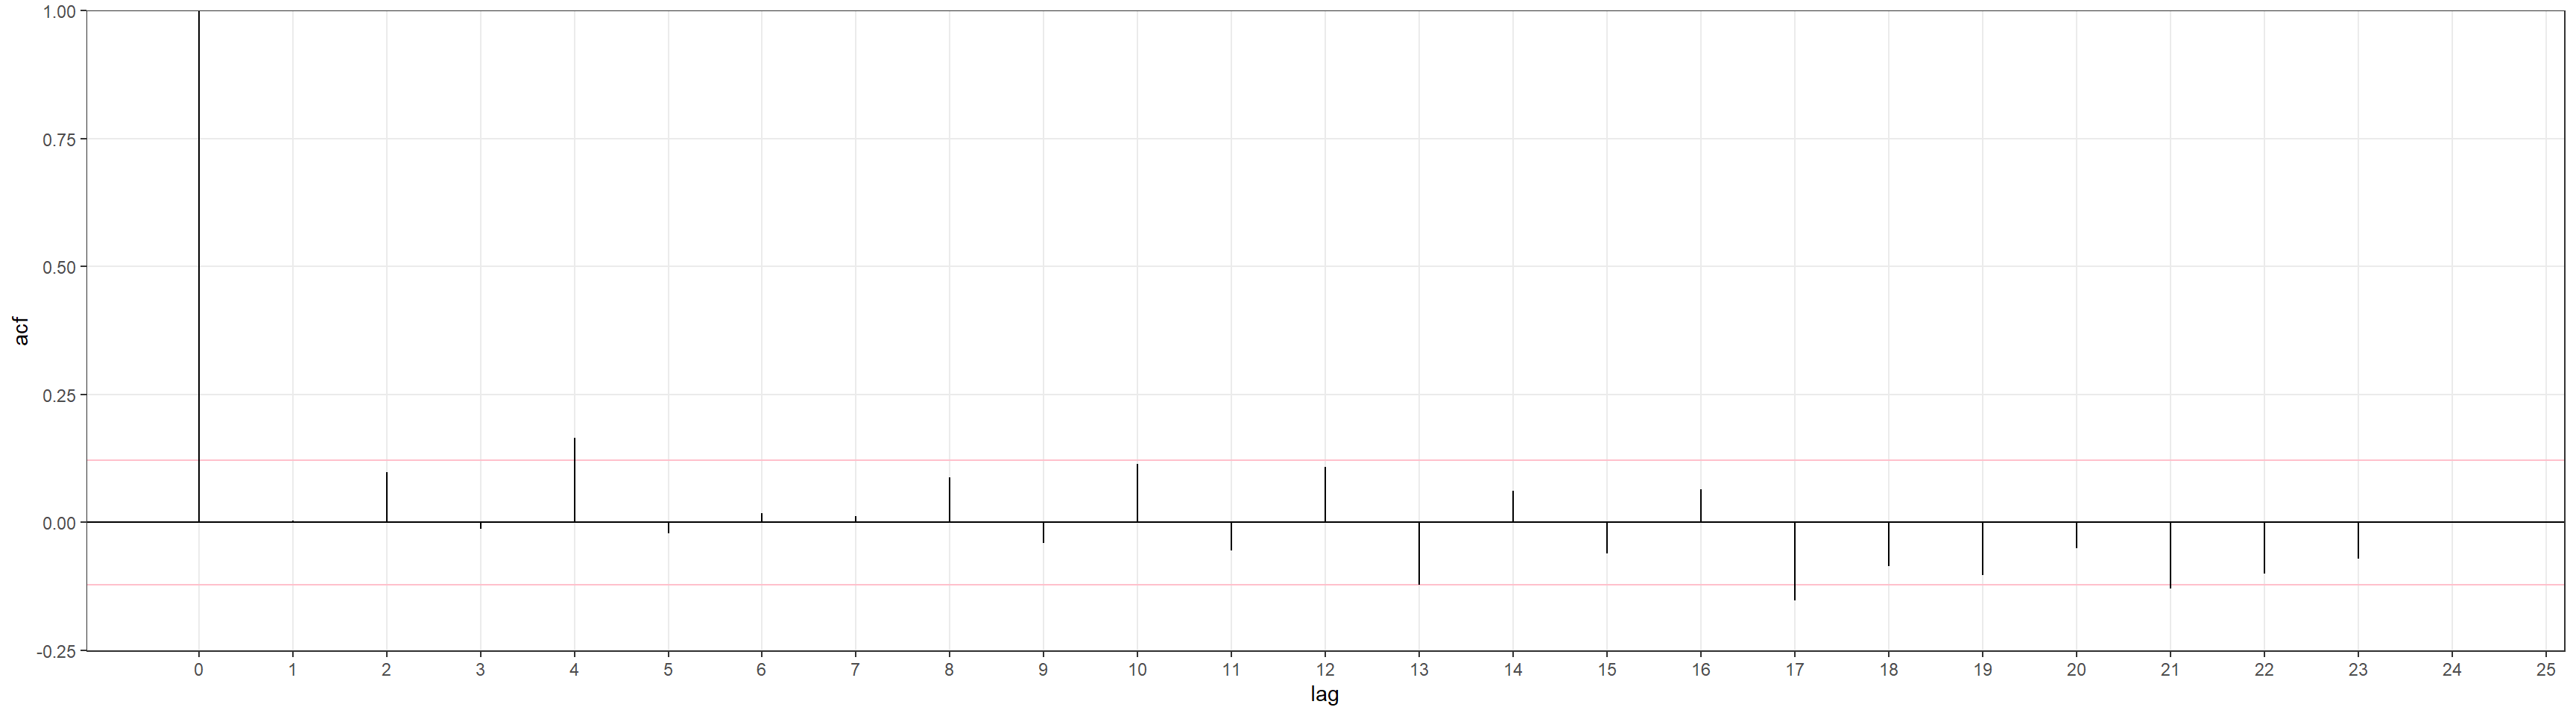
\includegraphics[width=1\linewidth]{Master_Thesis_Andreas_Kracht_Frandsen_files/figure-latex/SMB-AK-1} 

}

\caption{Autokorrelation af Small Minus Big.}\label{fig:SMB-AK}
\end{figure}

\begin{figure}[H]

{\centering 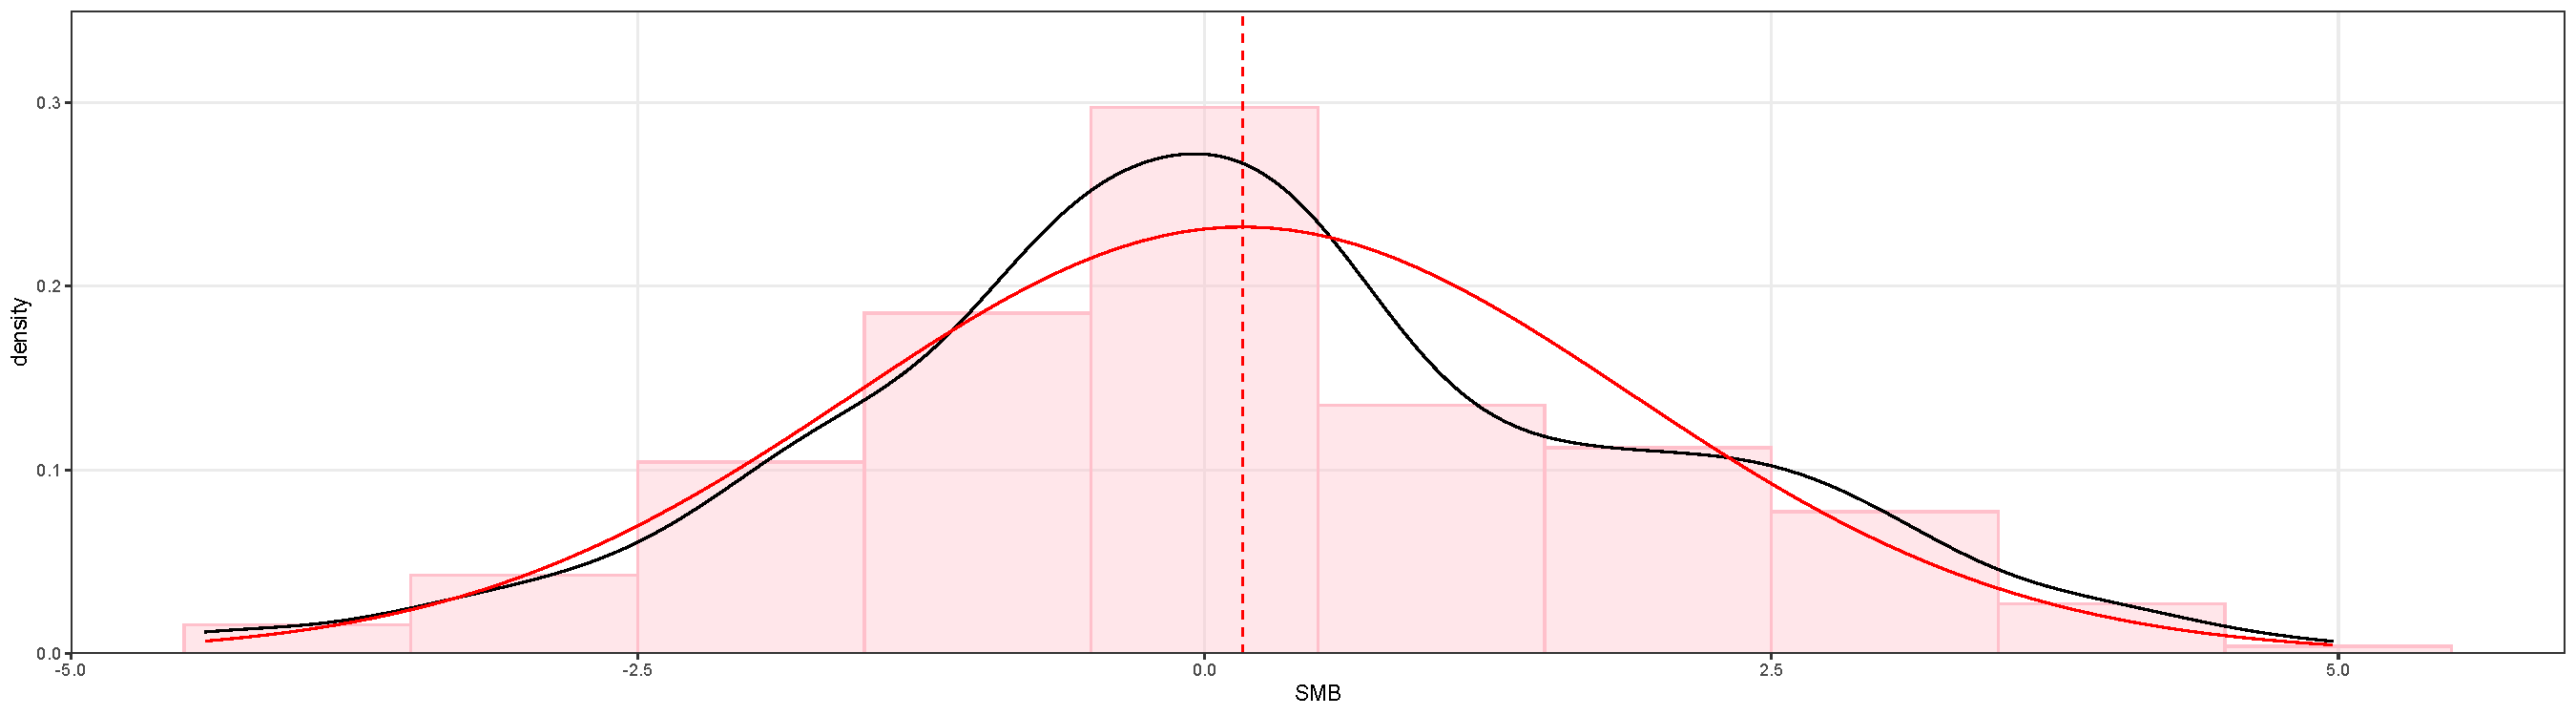
\includegraphics[width=1\linewidth]{Master_Thesis_Andreas_Kracht_Frandsen_files/figure-latex/SMB-HIST-1} 

}

\caption{Histogram for Small Minus Big.}\label{fig:SMB-HIST}
\end{figure}

\hypertarget{nominel-rente-x_ttextb}{%
\subsection{\texorpdfstring{Nominel rente -- \(x_t^{\text{b}}\)}{Nominel rente -- x\_t\^{}\{\textbackslash text\{b\}\}}}\label{nominel-rente-x_ttextb}}

Det kvartalsvise log brutto afkast på den amerikanske 90-dages \emph{T-Bill} benyttes som en proxy for den nominelle rente. Ved at inkludere både brutto og netto log renten, inkorporeres inflation. Eftersom log inflation er forskellen mellem log brutto renten og log netto renten. Data er fra \citep{CRSPt90} og hentet gennem \citep{WRDSt90}. Den justerede middelværdi estimeres til 1.173\(\%\). Volatiliteten estimeres til 0.837\(\%\). Tredje og fjerde moment estimeres til hhv. 0.903 og 4.313. Figur \ref{fig:B-tids} viser et plot over tidsserien, Figur \ref{fig:B-AK} viser et plot over autokorrelationen for tidsserien og Figur \ref{fig:B-HIST} viser et plot over histogrammet for tidsserien med tilhørende \emph{kernel} tæthed samt tæthed for en normalfordelt stokastisk variabel med middelværdi og standard afvigelse lig ovenstående estimater.

\begin{figure}[H]

{\centering 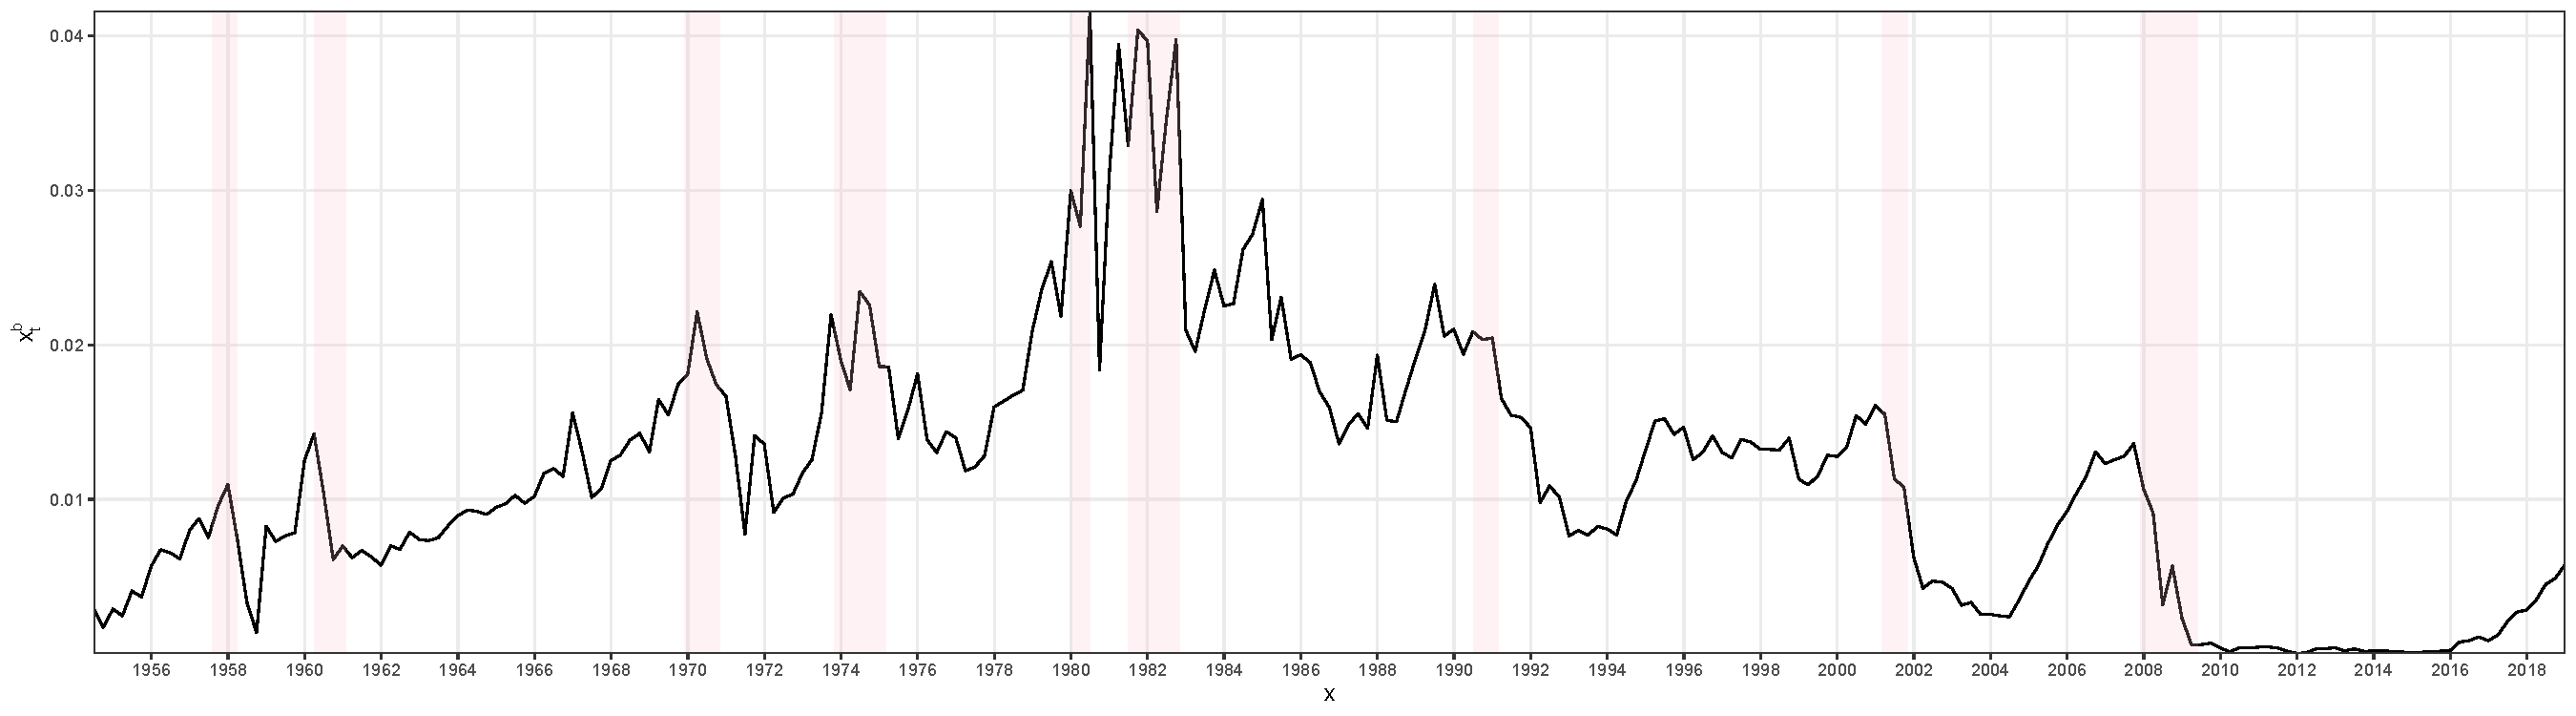
\includegraphics[width=1\linewidth]{Master_Thesis_Andreas_Kracht_Frandsen_files/figure-latex/B-tids-1} 

}

\caption{Tidsserie af log brutto afkastet på det risikofrie aktiv.}\label{fig:B-tids}
\end{figure}

\begin{figure}[H]

{\centering 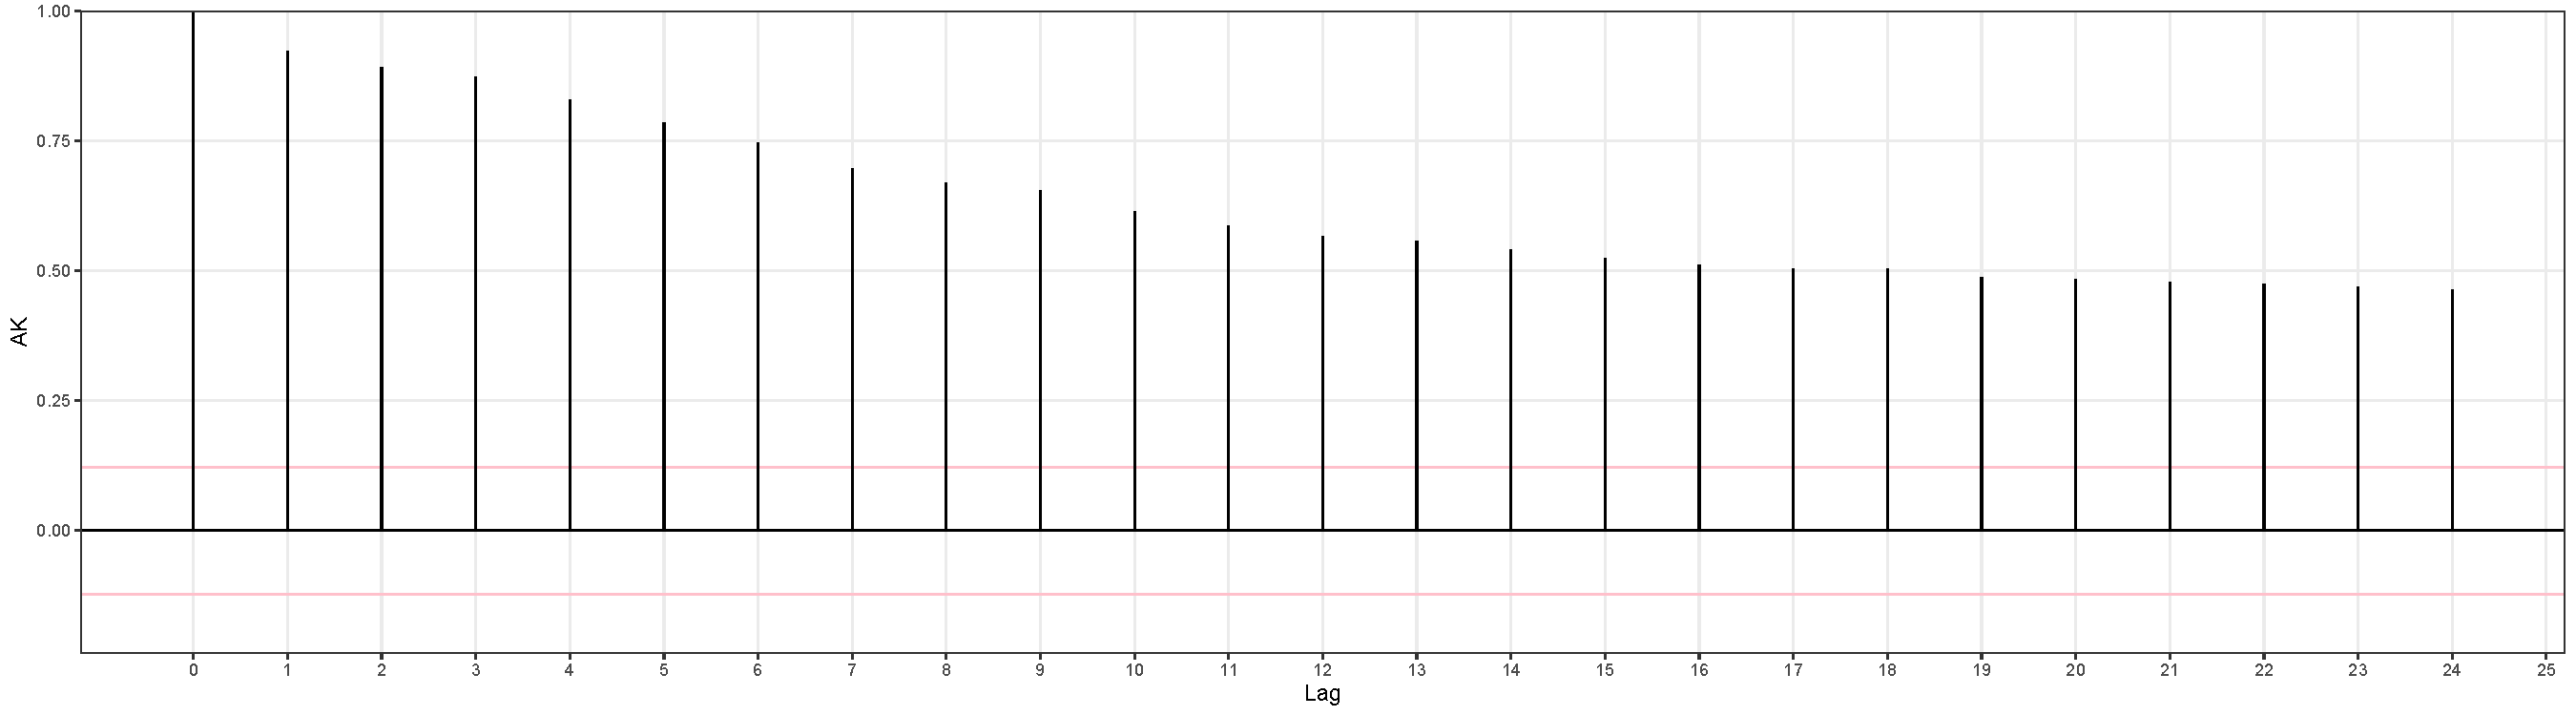
\includegraphics[width=1\linewidth]{Master_Thesis_Andreas_Kracht_Frandsen_files/figure-latex/B-AK-1} 

}

\caption{Autokorrelation af log brutto afkastet på det risikofrie aktiv.}\label{fig:B-AK}
\end{figure}

\begin{figure}[H]

{\centering 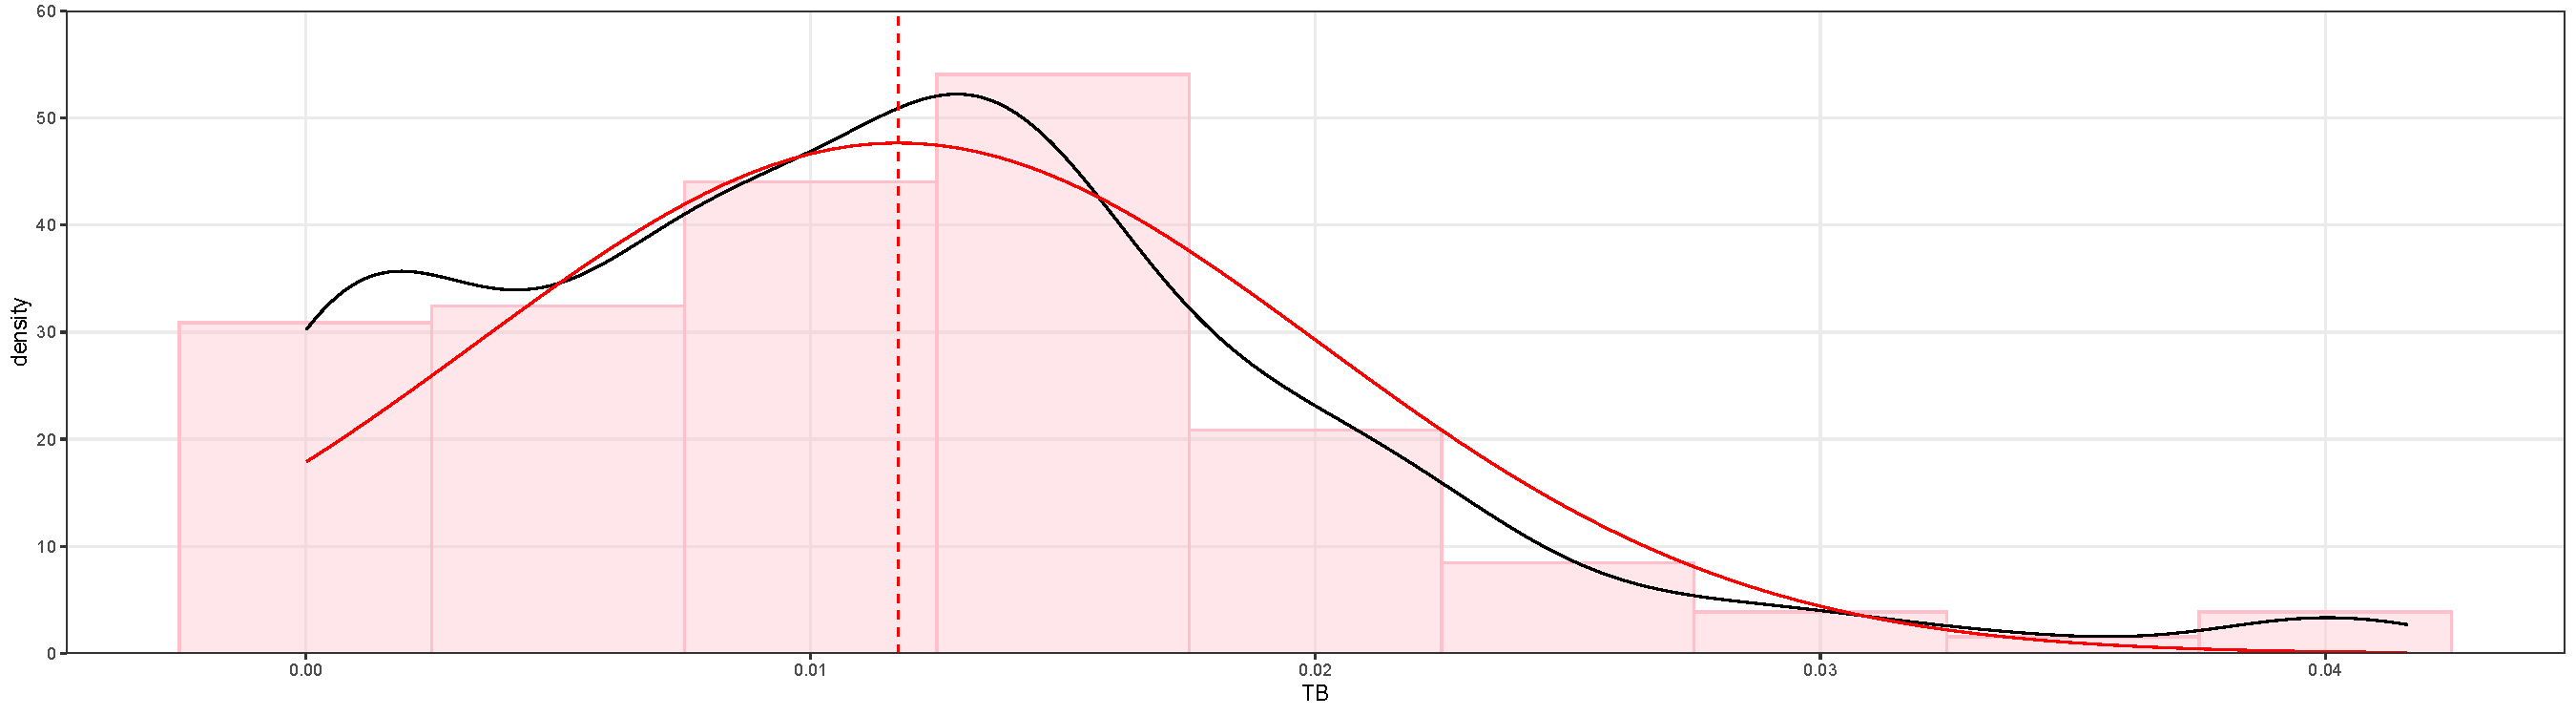
\includegraphics[width=1\linewidth]{Master_Thesis_Andreas_Kracht_Frandsen_files/figure-latex/B-HIST-1} 

}

\caption{Histogram for log brutto afkastet på det risikofrie aktiv.}\label{fig:B-HIST}
\end{figure}

\hypertarget{term-spread-x_ttextts}{%
\subsection{\texorpdfstring{Term Spread -- \(x_t^{\text{ts}}\)}{Term Spread -- x\_t\^{}\{\textbackslash text\{ts\}\}}}\label{term-spread-x_ttextts}}

For at beregne \emph{Term Spread} (rentespændet for den lange rente), benyttes den amerikanske \(10\)-årige effektive rente med konstant løbetid samt den 90-dages \emph{T-Bill} \emph{Secondary Market Rate}. Kvartalsvise data er hentet fra \citep{FRED102020} og \citep{FRED902020}, derudover er data ikke blevet sæsonjusteret. Spændet beregnes da som
\[x_t^{\text{ts}}=Y_t^{10}-Y_t^{90},\]

hvor \(Y_t^{10}\) og \(Y_t^{90}\) er de to effektive renter. Dette følger metoden fra \citep{Campbell1991}, som også argumenterer for, at ethvert rentespænd for renter med løbetider mellem \(1\) måned og \(10\) år, kan prædiktere rentestrukturen. Middelværdien for det lange rentespænd estimeres til 1.469\(\%\). Volatiliteten estimeres til 1.186\(\%\). Fordelingen er forholdsvis symmetrisk med skævhed og kurtosis på hhv. -0.231 og 3.033. Figur \ref{fig:TS-tids} viser et plot over tidsserien, Figur \ref{fig:TS-AK} viser et plot over autokorrelationen for tidsserien og Figur \ref{fig:TS-HIST} viser et plot over histogrammet for tidsserien med tilhørende \emph{kernel} tæthed samt tæthed for en normalfordelt stokastisk variabel med middelværdi og standard afvigelse lig ovenstående estimater.

\begin{figure}[H]

{\centering 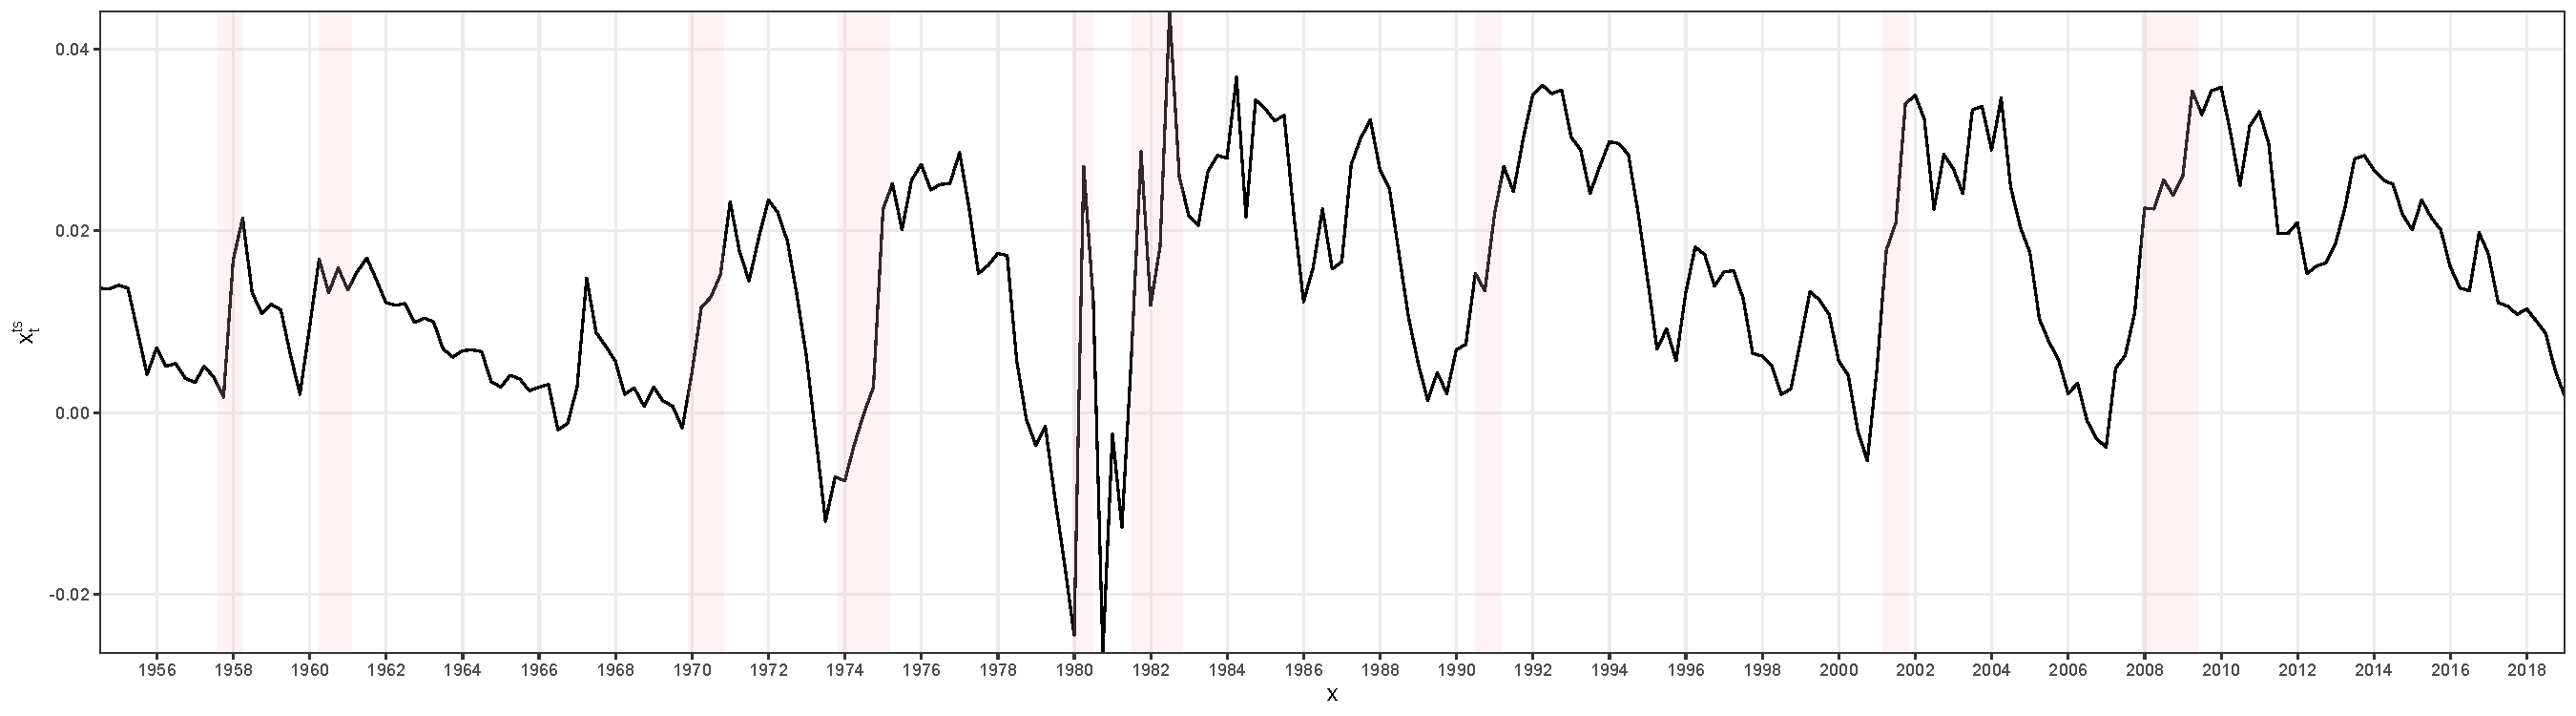
\includegraphics[width=1\linewidth]{Master_Thesis_Andreas_Kracht_Frandsen_files/figure-latex/TS-tids-1} 

}

\caption{Tidsserie af Term Spread.}\label{fig:TS-tids}
\end{figure}

\begin{figure}[H]

{\centering 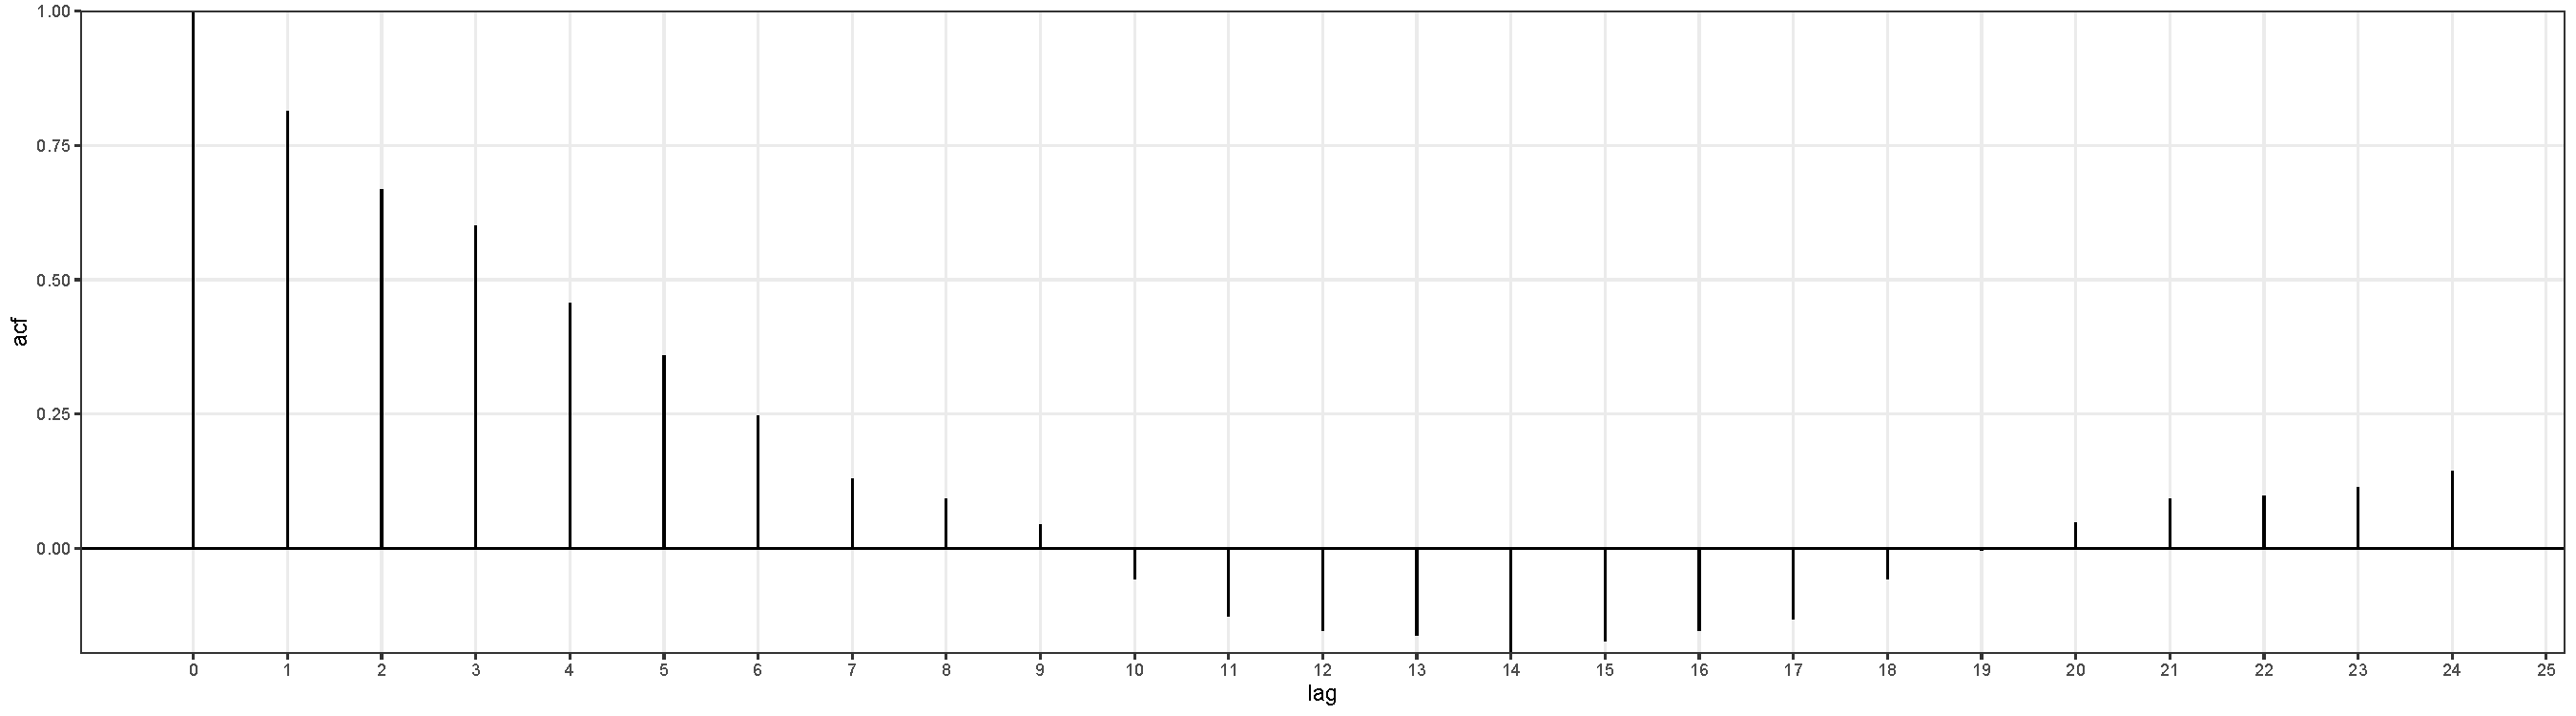
\includegraphics[width=1\linewidth]{Master_Thesis_Andreas_Kracht_Frandsen_files/figure-latex/TS-AK-1} 

}

\caption{Autokorrelation af Term Spread.}\label{fig:TS-AK}
\end{figure}

\begin{figure}[H]

{\centering 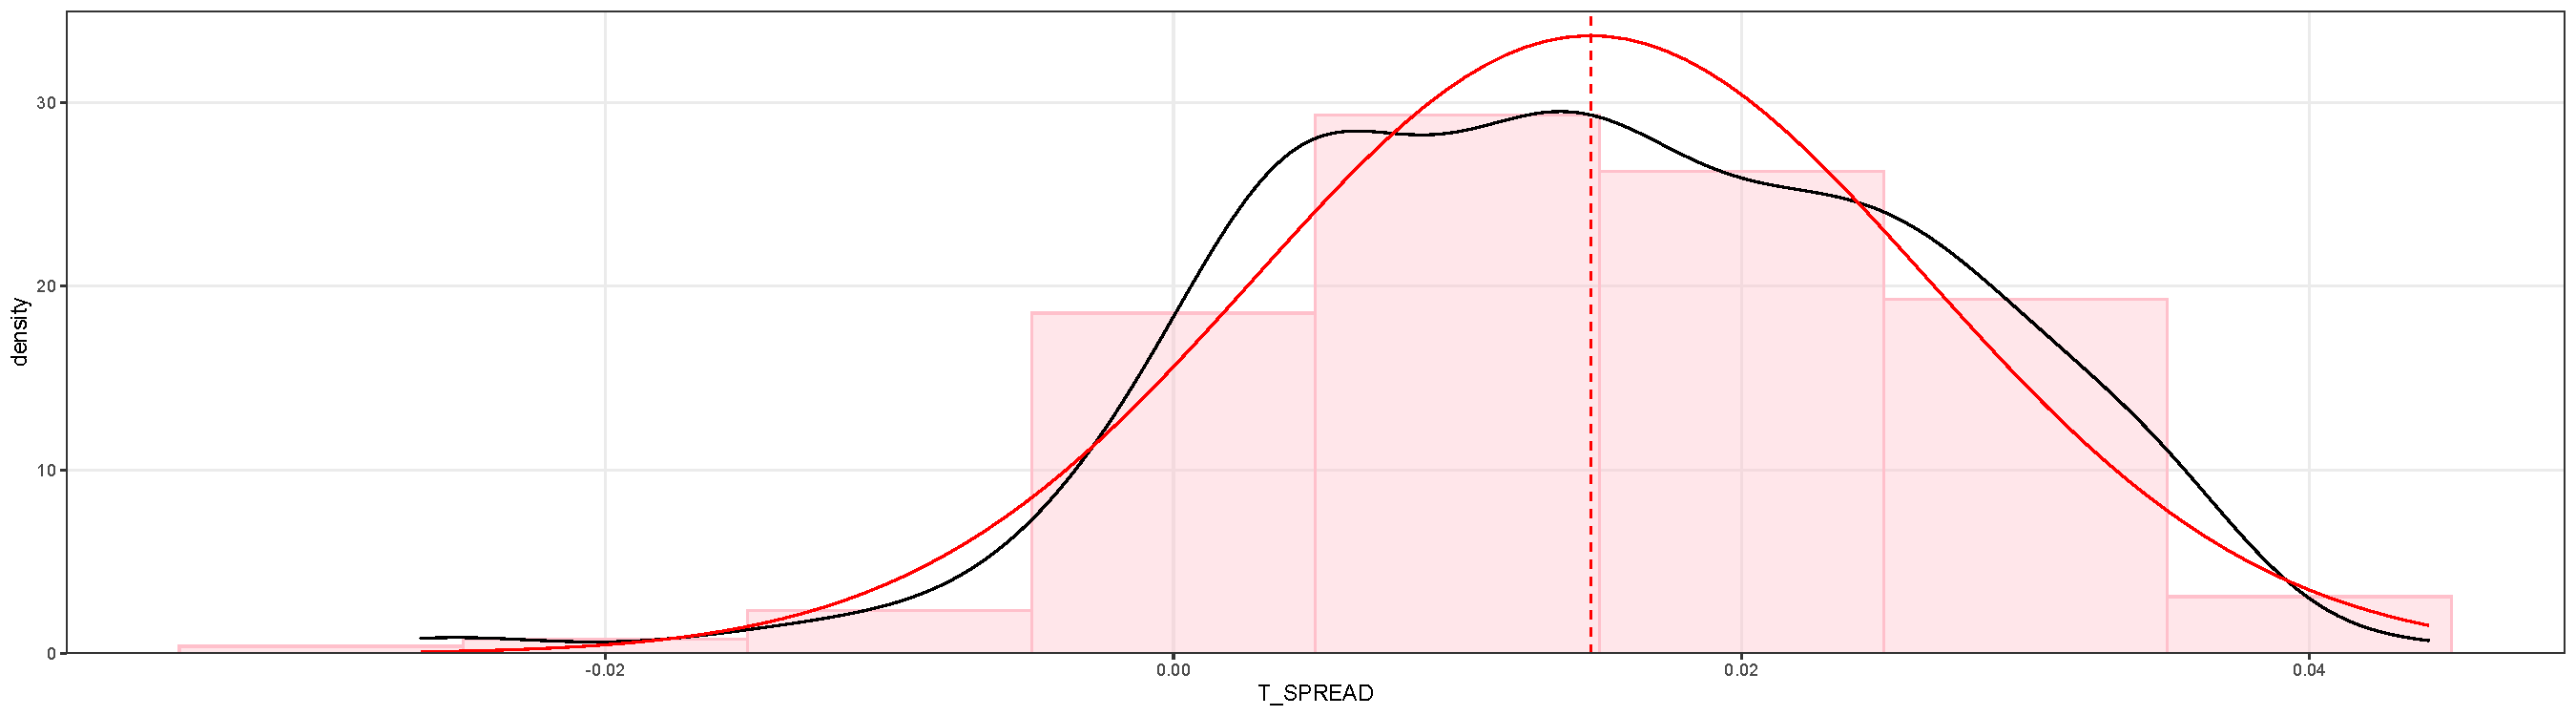
\includegraphics[width=1\linewidth]{Master_Thesis_Andreas_Kracht_Frandsen_files/figure-latex/TS-HIST-1} 

}

\caption{Histogram for Term Spread.}\label{fig:TS-HIST}
\end{figure}

\hypertarget{yield-spread-x_ttextys}{%
\subsection{\texorpdfstring{Yield Spread -- \(x_t^{\text{ys}}\)}{Yield Spread -- x\_t\^{}\{\textbackslash text\{ys\}\}}}\label{yield-spread-x_ttextys}}

Datagrundlaget for \emph{Yield Spread} (rentespændet for den korte rente) er den amerikanske \(10\)-årige effektive rente med konstant løbetid samt den 90-dages \emph{T-Bill} \emph{Secondary Market Rate}. Kvartalsvise data er hentet fra \citep{FRED52020} og \citep{FRED902020}, og er ikke sæsonjusteret. Spændet beregnes da som
\[x_t^{\text{ts}}=Y_t^{5}-Y_t^{90},\]

hvor \(Y_t^{5}\) og \(Y_t^{90}\) er de to effektive renter. Middelværdien, 1.166\(\%\), er som forventet en anelse mindre end middelværdien for \emph{Term Spread}. Det samme er volatiliteten, 0.927\(\%\). Fordelingen er en anelse leptokurtisk med kurtosis på 3.828. Skævheden er -0.153. Figur \ref{fig:YS-tids} viser et plot over tidsserien, Figur \ref{fig:YS-AK} viser et plot over autokorrelationen for tidsserien og Figur \ref{fig:YS-HIST} viser et plot over histogrammet for tidsserien med tilhørende \emph{kernel} tæthed samt tæthed for en normalfordelt stokastisk variabel med middelværdi og standard afvigelse lig ovenstående estimater.

\begin{figure}[H]

{\centering 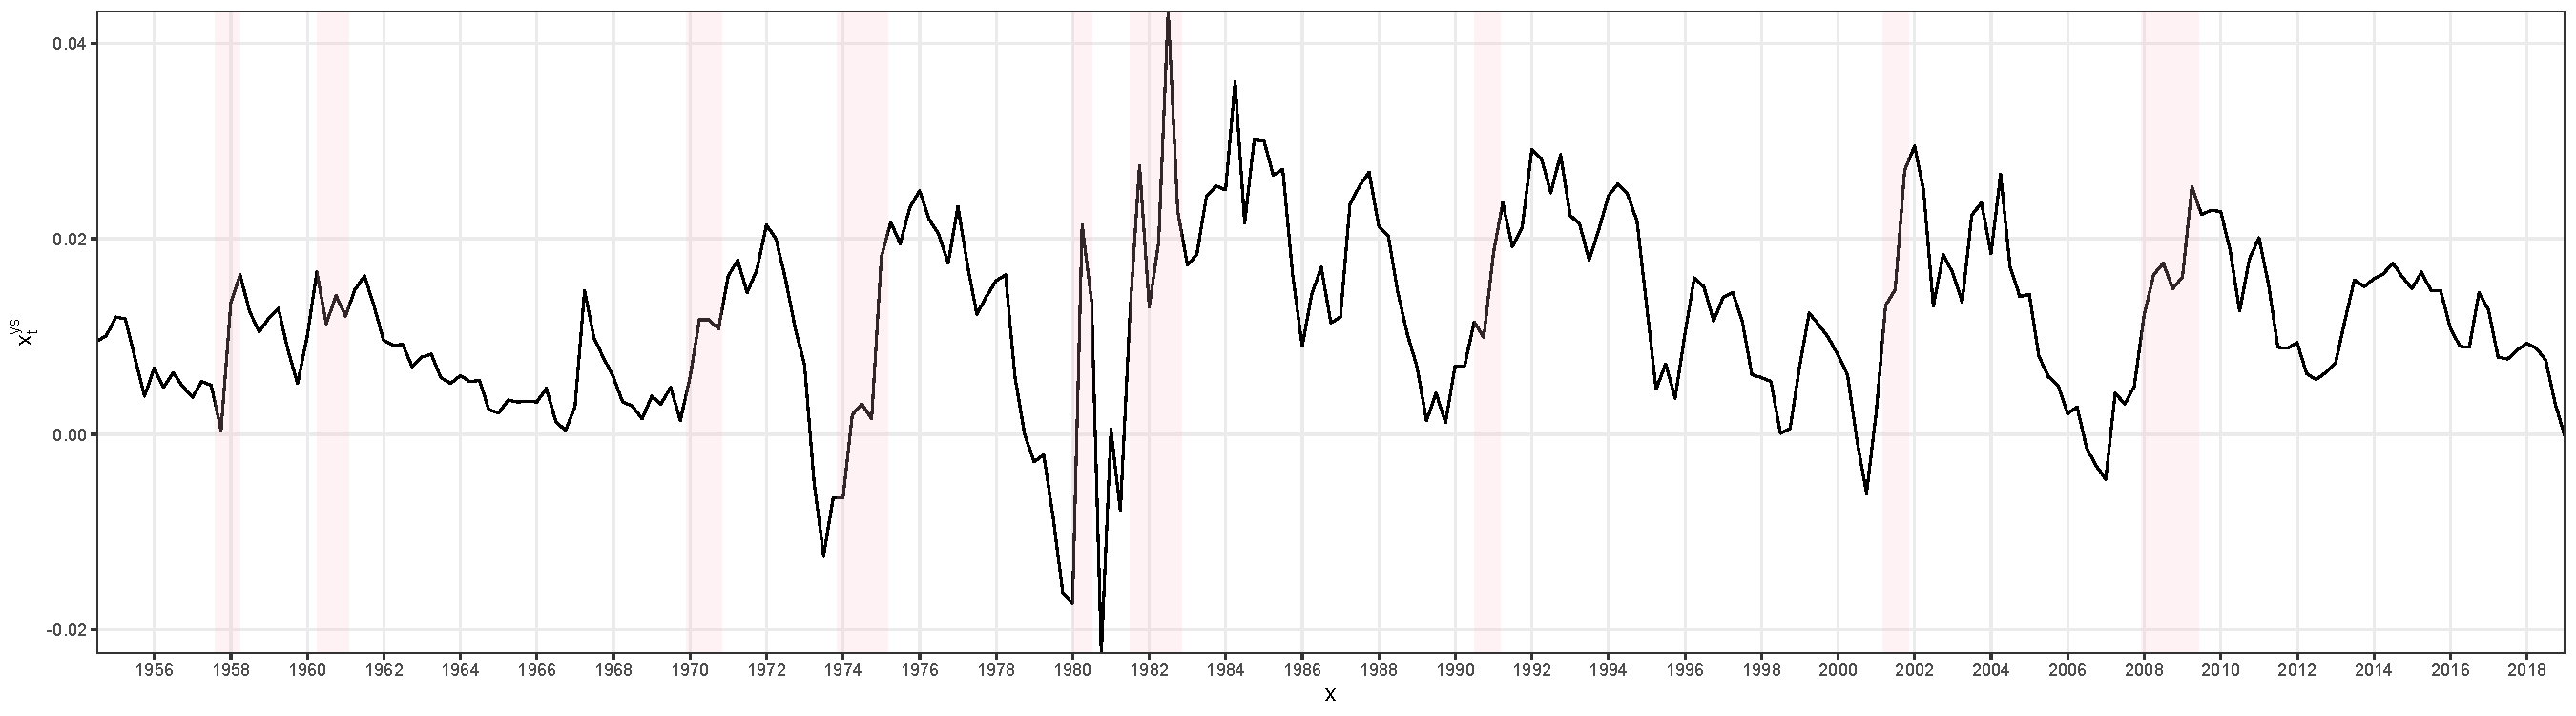
\includegraphics[width=1\linewidth]{Master_Thesis_Andreas_Kracht_Frandsen_files/figure-latex/YS-tids-1} 

}

\caption{Tidsserie af Yield Spread.}\label{fig:YS-tids}
\end{figure}

\begin{figure}[H]

{\centering 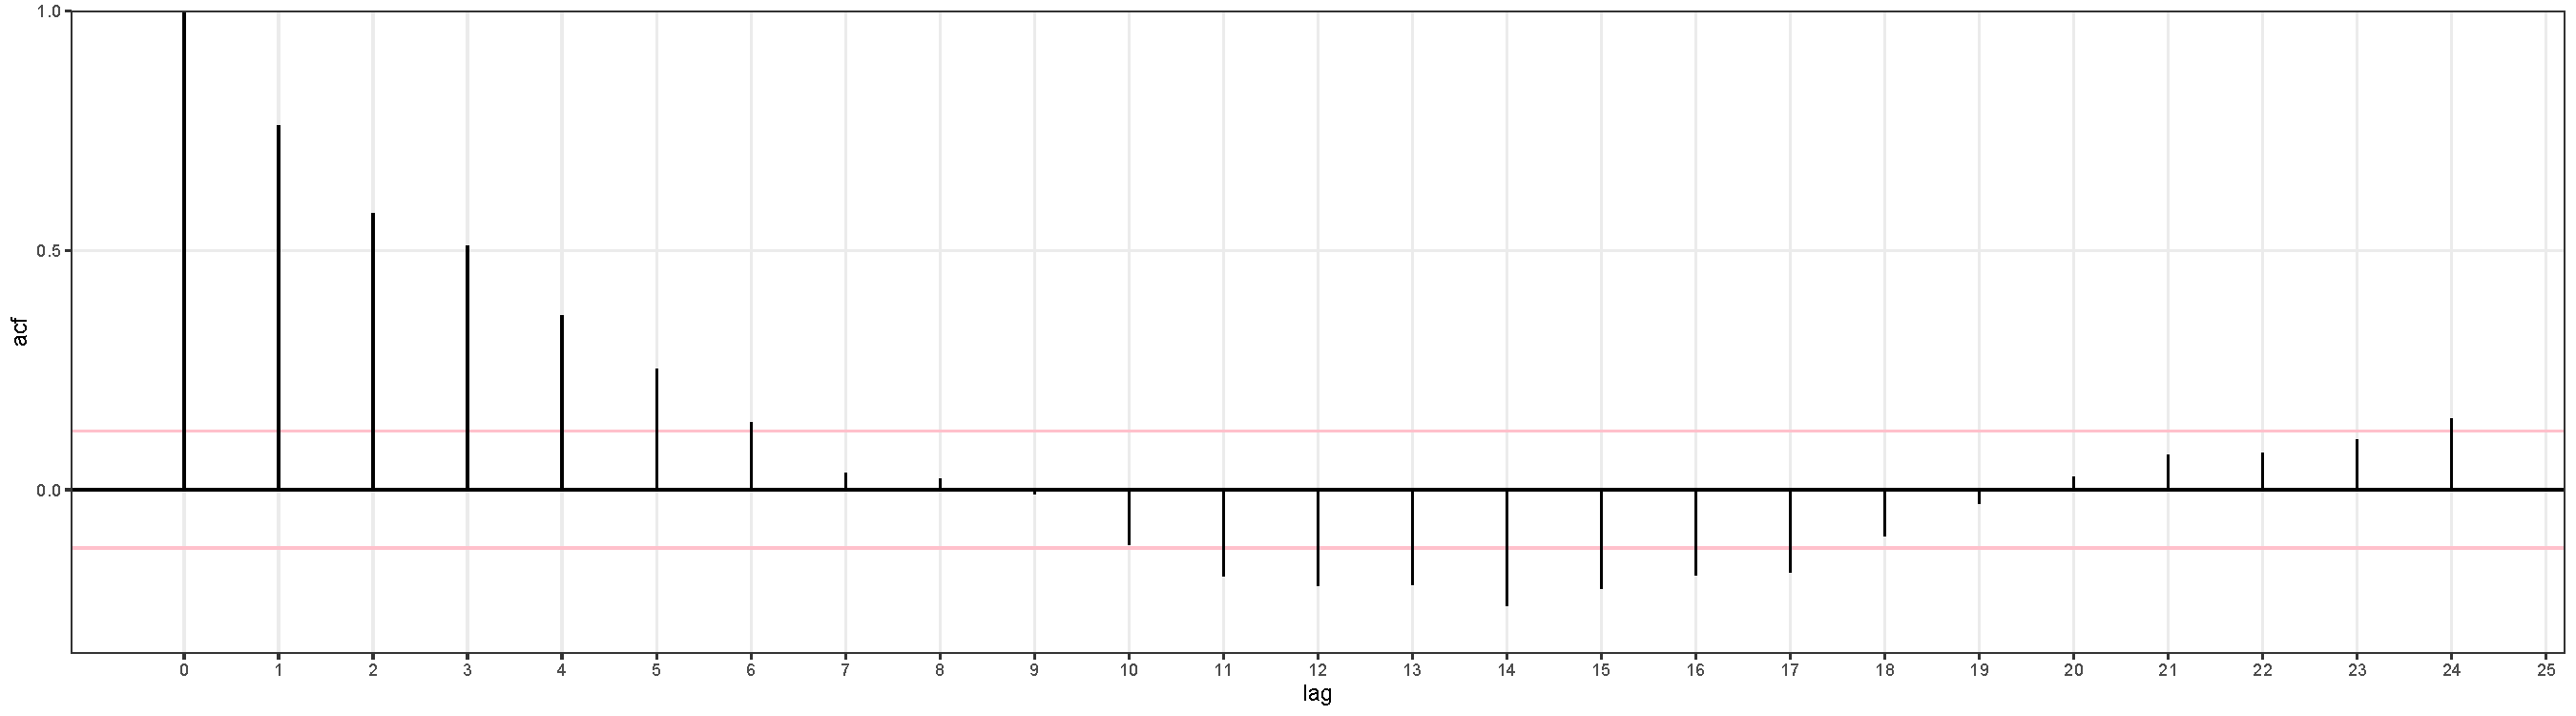
\includegraphics[width=1\linewidth]{Master_Thesis_Andreas_Kracht_Frandsen_files/figure-latex/YS-AK-1} 

}

\caption{Autokorrelation af Yield Spread.}\label{fig:YS-AK}
\end{figure}

\begin{figure}[H]

{\centering 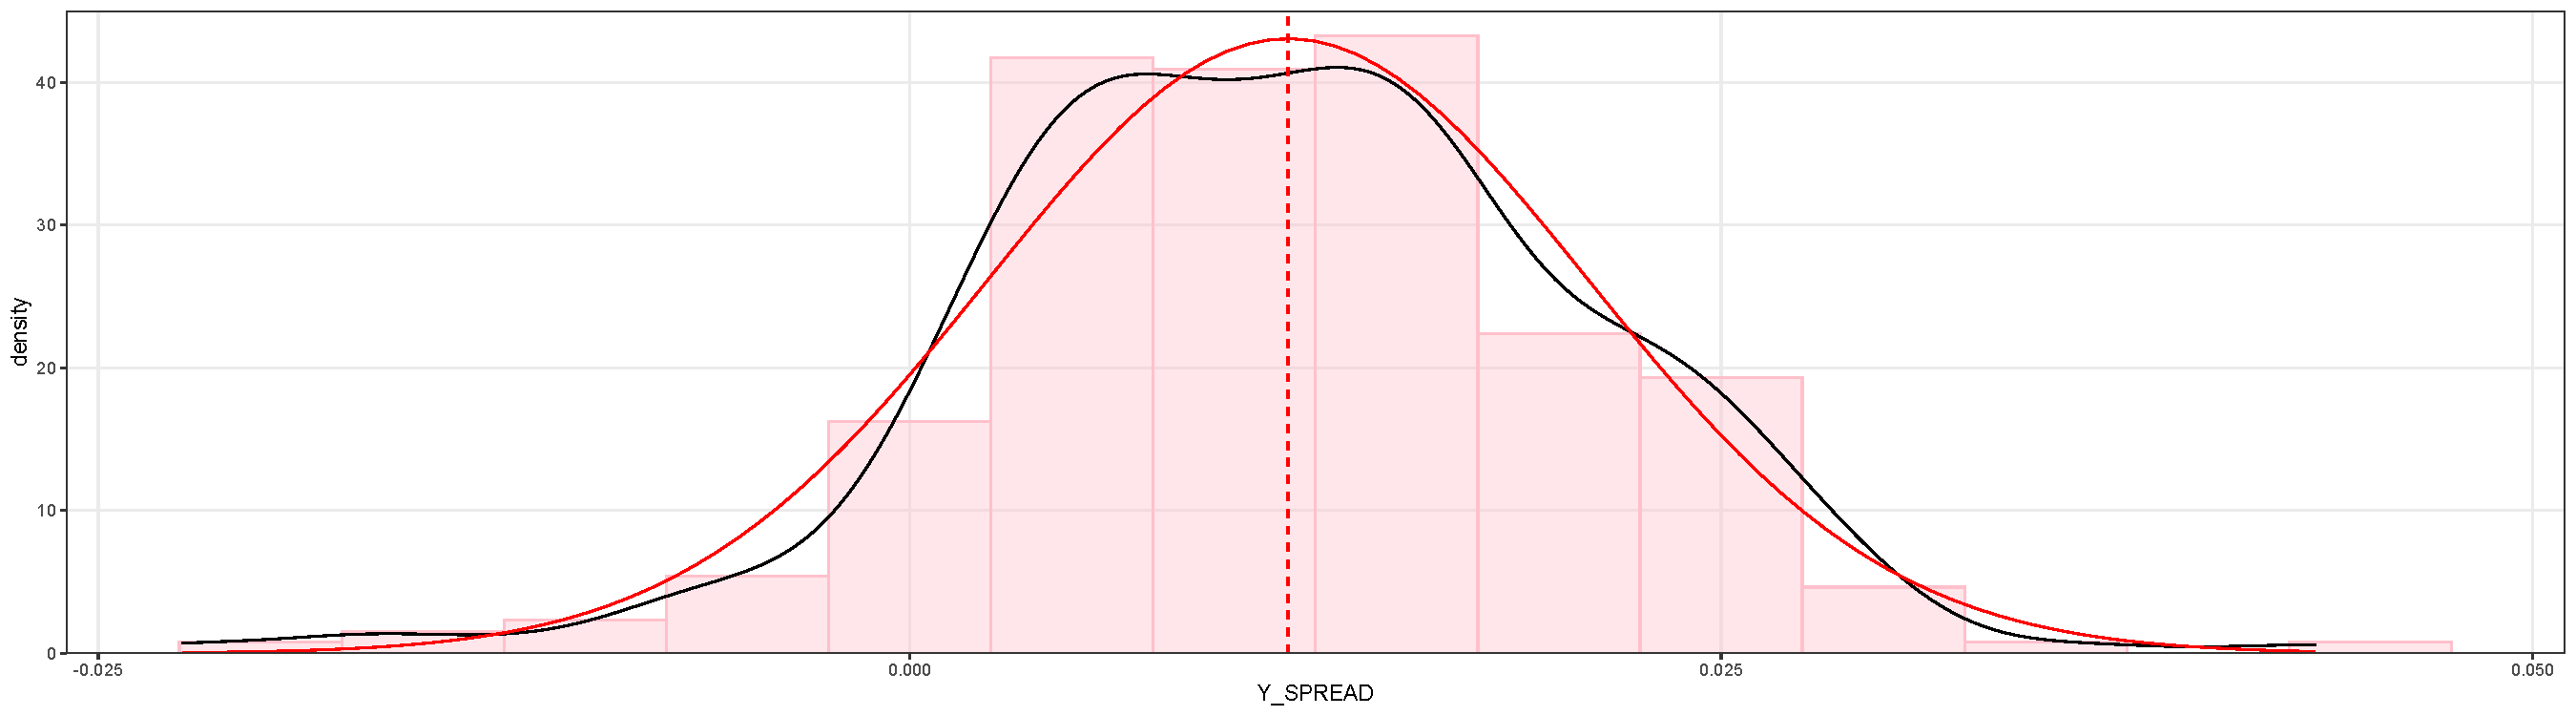
\includegraphics[width=1\linewidth]{Master_Thesis_Andreas_Kracht_Frandsen_files/figure-latex/YS-HIST-1} 

}

\caption{Histogram for Yield Spread.}\label{fig:YS-HIST}
\end{figure}

\hypertarget{credit-spread-x_ttextcs}{%
\subsection{\texorpdfstring{Credit Spread -- \(x_t^{\text{cs}}\)}{Credit Spread -- x\_t\^{}\{\textbackslash text\{cs\}\}}}\label{credit-spread-x_ttextcs}}

Beregningen til \emph{Credit Spread} (kreditspændet) benytter den 90-dages \emph{T-Bill} \emph{Secondary Market Rate} samt den effektive rente fra \emph{Moody's Seasoned BAA Corporate Bond}, og baserer sig på instrumenter med løbetider på \(20\) år eller mere. Data er hentet fra hhv. \citep{FRED902020} samt \citep{Goyal2007}. Metoden følger fra \citep{Keim1986}, og kreditspændet beregnes da som
\[x_t^{\text{cs}}=Y_t^{\text{BAA}}-Y_t^{90},\]

hvor \(Y_t^{\text{BAA}}\) og \(Y_t^{90}\) er de to effektive renter. Af de fem rentrestruktursvariable ses det, at kreditspændet har den højeste middelværdi på 3.398\(\%\), og en standardafvigelse på 1.732\(\%\). Tredje og fjerde moment estimeres til hhv. 0.159 og 2.33. Figur \ref{fig:CS-tids} viser et plot over tidsserien, Figur \ref{fig:CS-AK} viser et plot over autokorrelationen for tidsserien og Figur \ref{fig:CS-HIST} viser et plot over histogrammet for tidsserien med tilhørende \emph{kernel} tæthed samt tæthed for en normalfordelt stokastisk variabel med middelværdi og standard afvigelse lig ovenstående estimater.

\begin{figure}[H]

{\centering 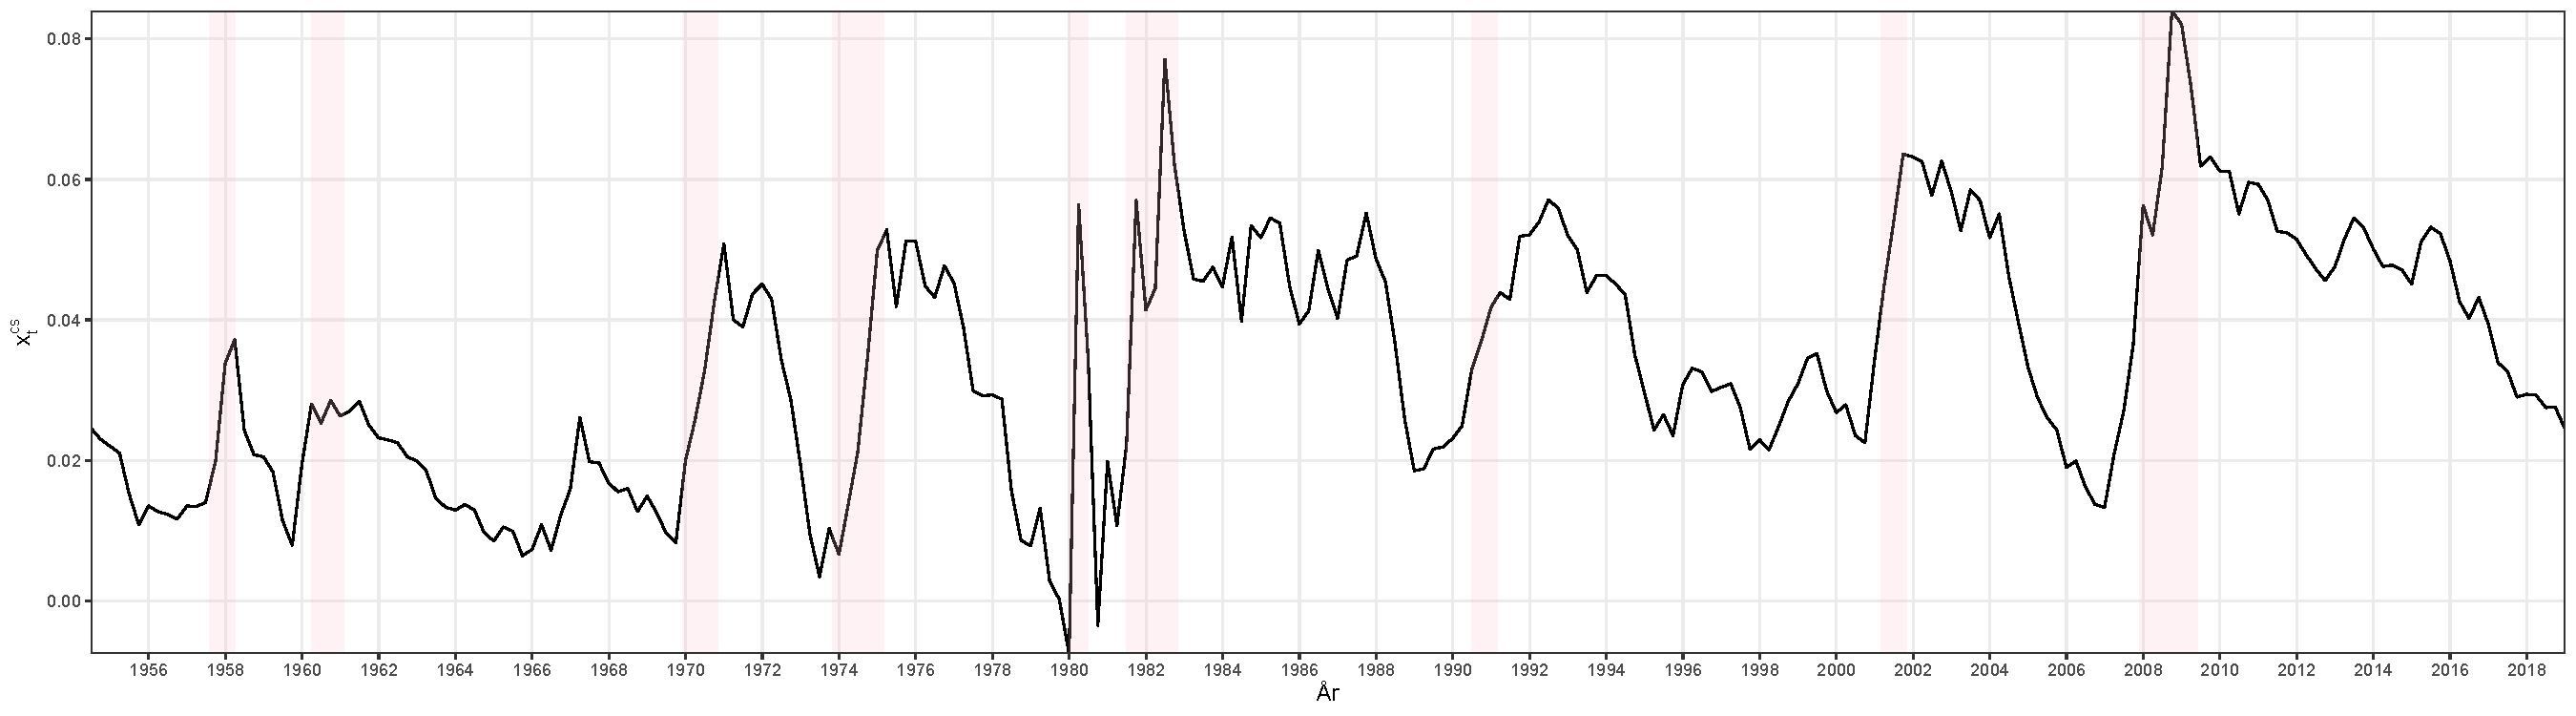
\includegraphics[width=1\linewidth]{Master_Thesis_Andreas_Kracht_Frandsen_files/figure-latex/CS-tids-1} 

}

\caption{Tidsserie af Credit Spread.}\label{fig:CS-tids}
\end{figure}

\begin{figure}[H]

{\centering 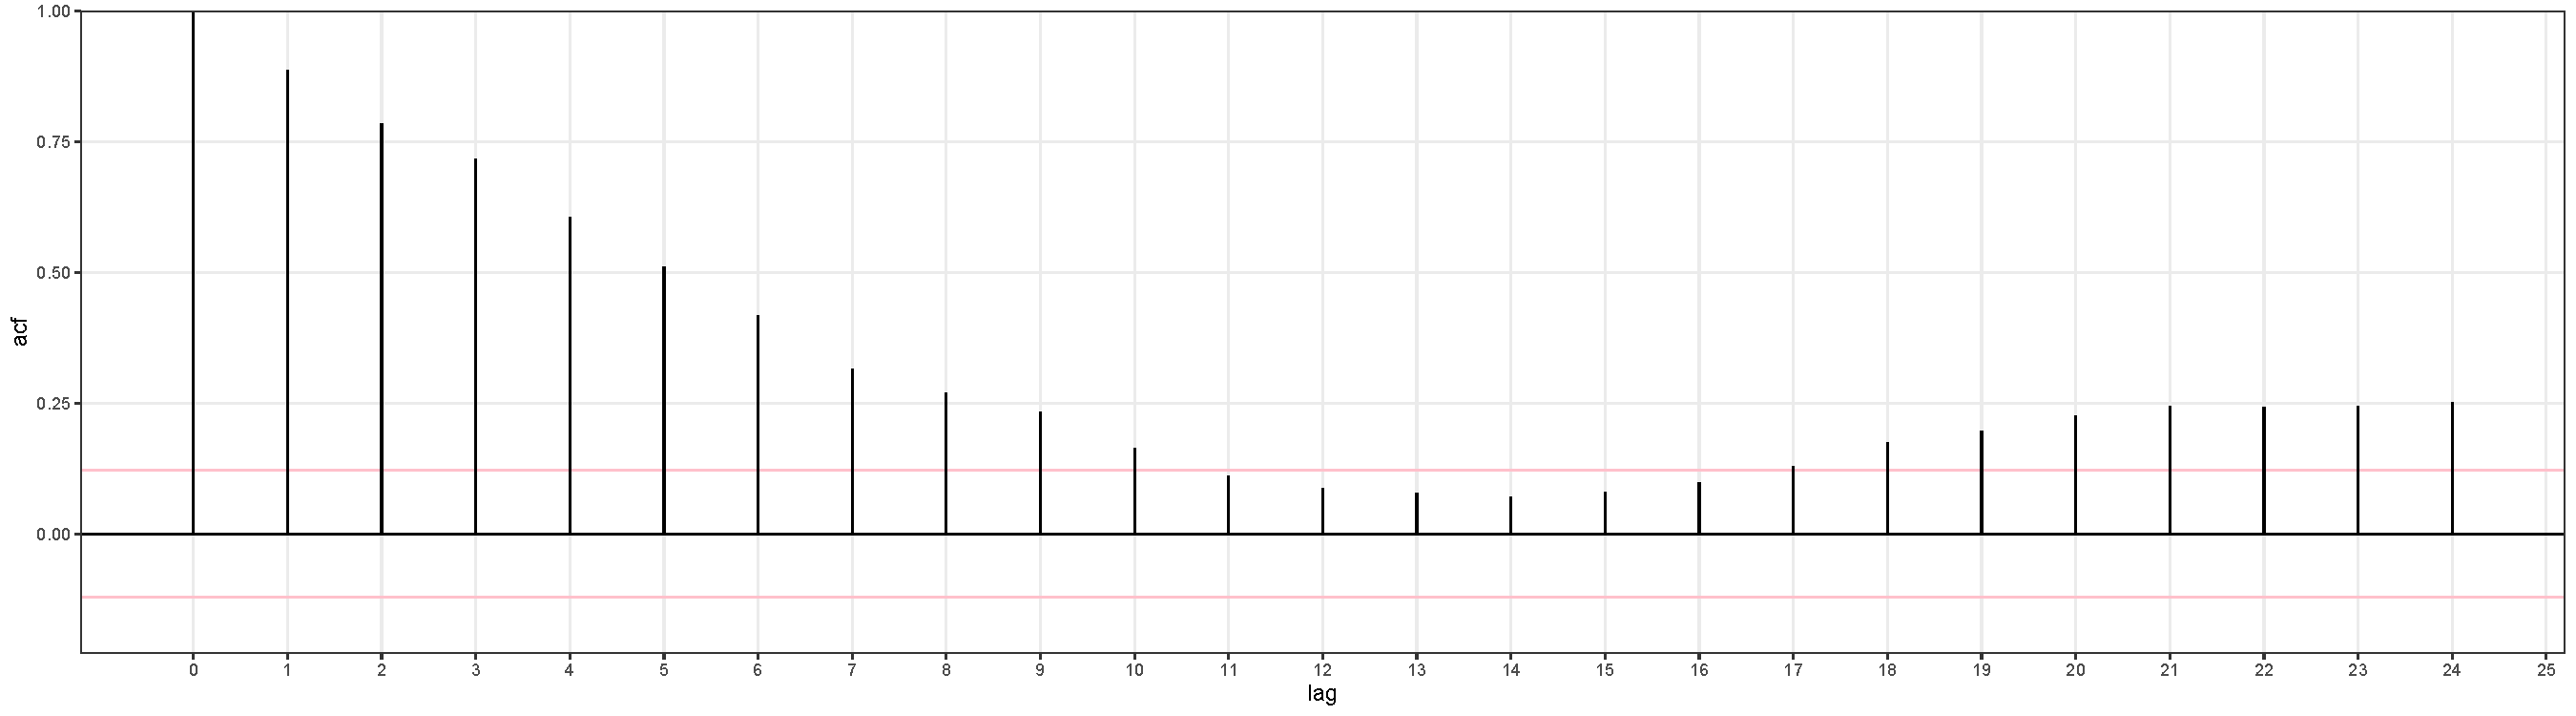
\includegraphics[width=1\linewidth]{Master_Thesis_Andreas_Kracht_Frandsen_files/figure-latex/CS-AK-1} 

}

\caption{Autokorrelation af Credit Spread.}\label{fig:CS-AK}
\end{figure}

\begin{figure}[H]

{\centering 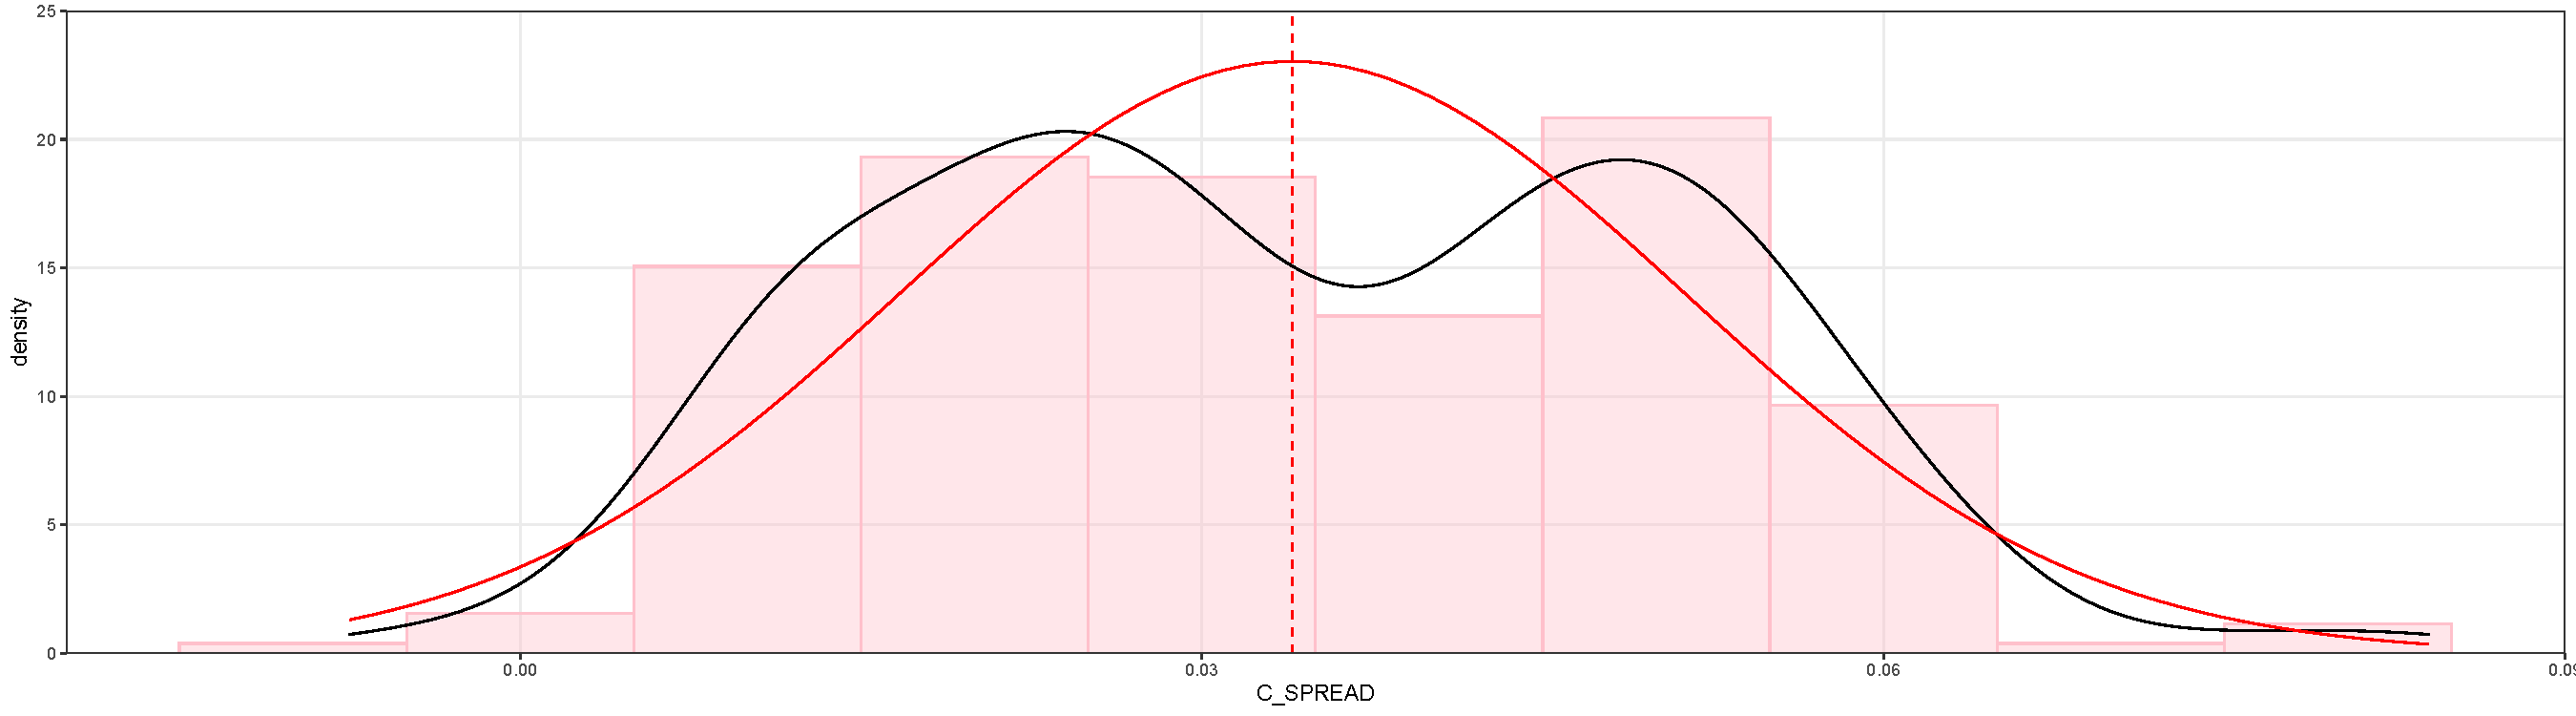
\includegraphics[width=1\linewidth]{Master_Thesis_Andreas_Kracht_Frandsen_files/figure-latex/CS-HIST-1} 

}

\caption{Histogram for Credit Spread.}\label{fig:CS-HIST}
\end{figure}

\hypertarget{default-spread-x_ttextds}{%
\subsection{\texorpdfstring{Default Spread -- \(x_t^{\text{ds}}\)}{Default Spread -- x\_t\^{}\{\textbackslash text\{ds\}\}}}\label{default-spread-x_ttextds}}

For at beregne \emph{Default Spread} (konkursspændet) benyttes den effektive rente fra \emph{Moody's Seasoned AAA Corporate Bond} samt den effektive rente fra \emph{Moody's Seasoned BAA Corporate Bond}, og baserer sig begge på instrumenter med løbetider på \(20\) år eller mere. Data er hentet via \citep{Goyal2007}. Konkursspændet beregnes da som
\[x_t^{\text{ds}}=Y_t^{\text{BAA}}-Y_t^{\text{AAA}},\]

hvor \(Y_t^{\text{BAA}}\) og \(Y_t^{\text{AAA}}\) er de to effektive renter. Til forskel for kreditspændet har konkursspændet den laveste middelværdi, 0.987\(\%\), også på tværs af de andre klasser af prædiktionsvariable. Standardafvigelsen er 0.439\(\%\). Af rentestruktursvariablene har konkursspændet også den hhv. mest ekstreme skævhed og kurtosis. Disse er hhv. 1.842 og 8.156, hvilket indebærer en højreskæv fordeling med tykke haler. Figur \ref{fig:DS-tids} viser et plot over tidsserien, Figur \ref{fig:DS-AK} viser et plot over autokorrelationen for tidsserien og Figur \ref{fig:DS-HIST} viser et plot over histogrammet for tidsserien med tilhørende \emph{kernel} tæthed samt tæthed for en normalfordelt stokastisk variabel med middelværdi og standard afvigelse lig ovenstående estimater.

\begin{figure}[H]

{\centering 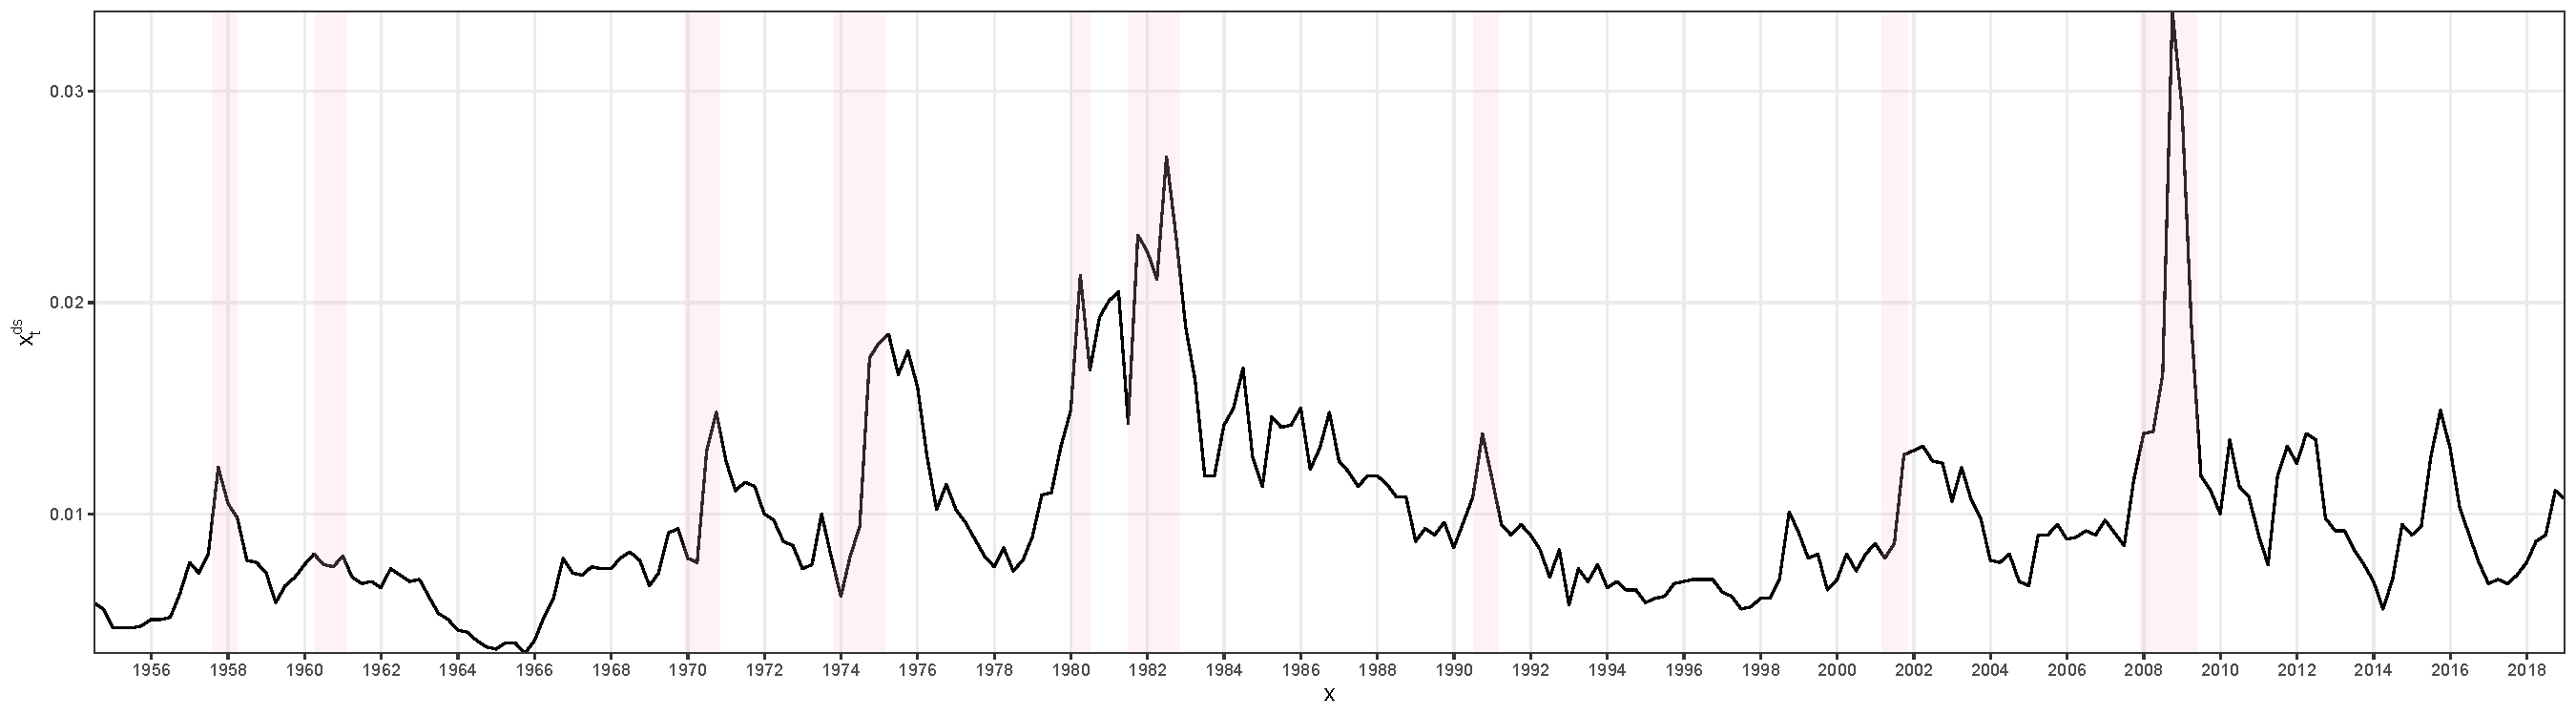
\includegraphics[width=1\linewidth]{Master_Thesis_Andreas_Kracht_Frandsen_files/figure-latex/DS-tids-1} 

}

\caption{Tidsserie af Default Spread.}\label{fig:DS-tids}
\end{figure}

\begin{figure}[H]

{\centering 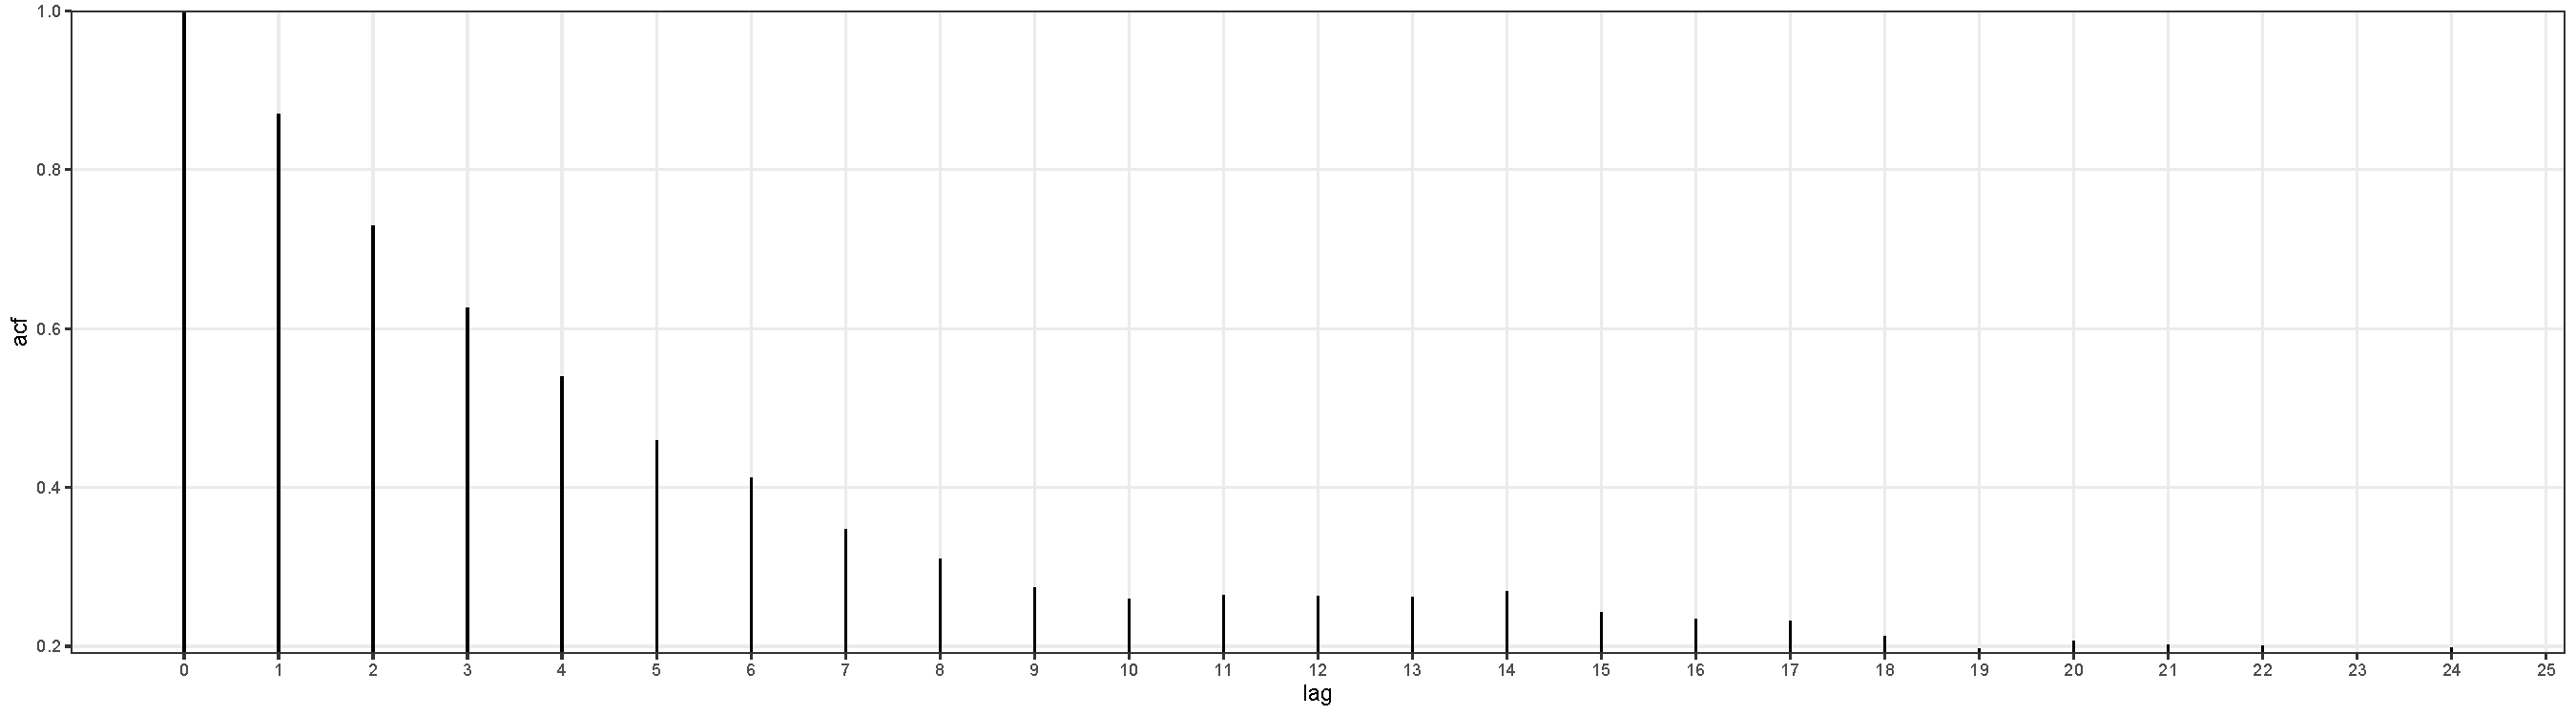
\includegraphics[width=1\linewidth]{Master_Thesis_Andreas_Kracht_Frandsen_files/figure-latex/DS-AK-1} 

}

\caption{Autokorrelation af Default Spread.}\label{fig:DS-AK}
\end{figure}

\begin{figure}[H]

{\centering 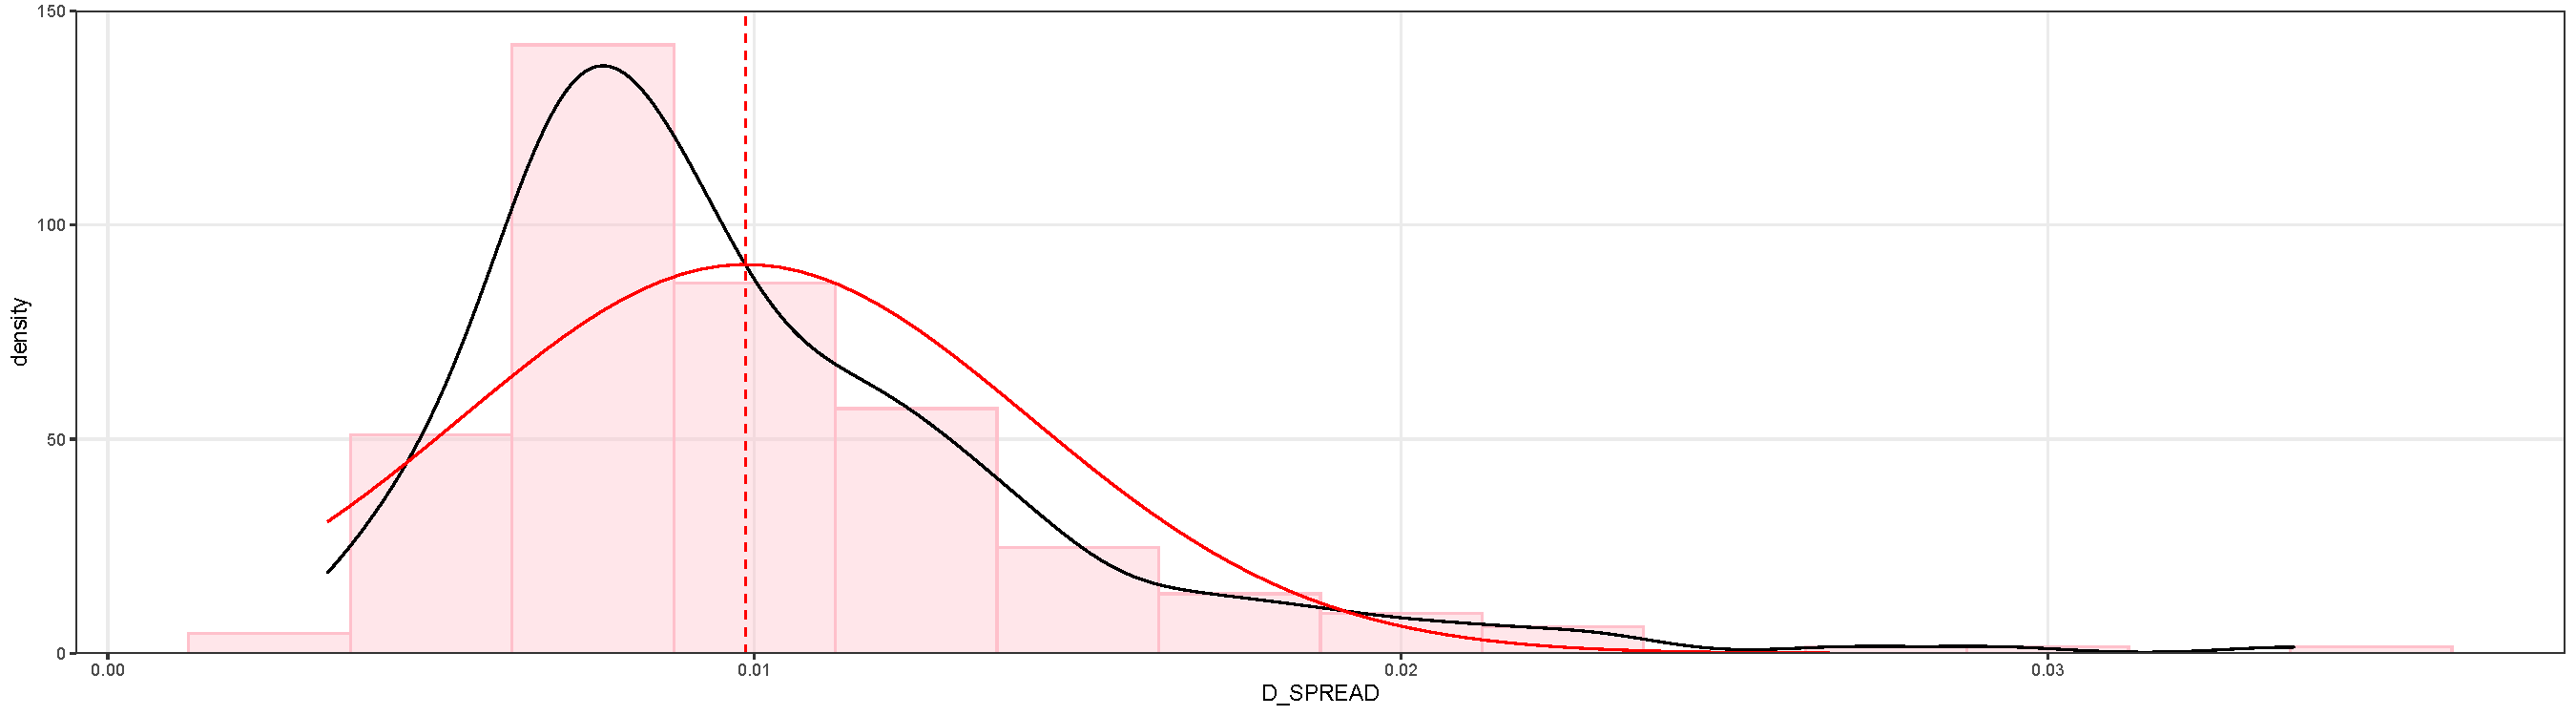
\includegraphics[width=1\linewidth]{Master_Thesis_Andreas_Kracht_Frandsen_files/figure-latex/DS-HIST-1} 

}

\caption{Histogram for Default Spread.}\label{fig:DS-HIST}
\end{figure}

\hypertarget{federal-funds-rate-x_ttextfr}{%
\subsection{\texorpdfstring{Federal Funds Rate -- \(x_t^{\text{fr}}\)}{Federal Funds Rate -- x\_t\^{}\{\textbackslash text\{fr\}\}}}\label{federal-funds-rate-x_ttextfr}}

I U.S.A. er \emph{Federal Funds Rate}, renten som private finansinstitutioner tager for at låne uden sikkerhed, sædvanligvis over natten, af finansinstitutions reserver i \emph{Federal Reserve Bank}. Data er hentet fra \citep{FREDF2020}. De kvartalsvis observationer er baseret på et gennemsnit af daglige observationer. Middelværdien er på 4.814\(\%\), og standardafvigelsen er på 3.606\(\%\). Tredje og fjerde moment estimeres til hhv. 1.053 og 4.625. Figur \ref{fig:FR-tids} viser et plot over tidsserien, Figur \ref{fig:FR-AK} viser et plot over autokorrelationen for tidsserien og Figur \ref{fig:FR-HIST} viser et plot over histogrammet for tidsserien med tilhørende \emph{kernel} tæthed samt tæthed for en normalfordelt stokastisk variabel med middelværdi og standard afvigelse lig ovenstående estimater.

\begin{figure}[H]

{\centering 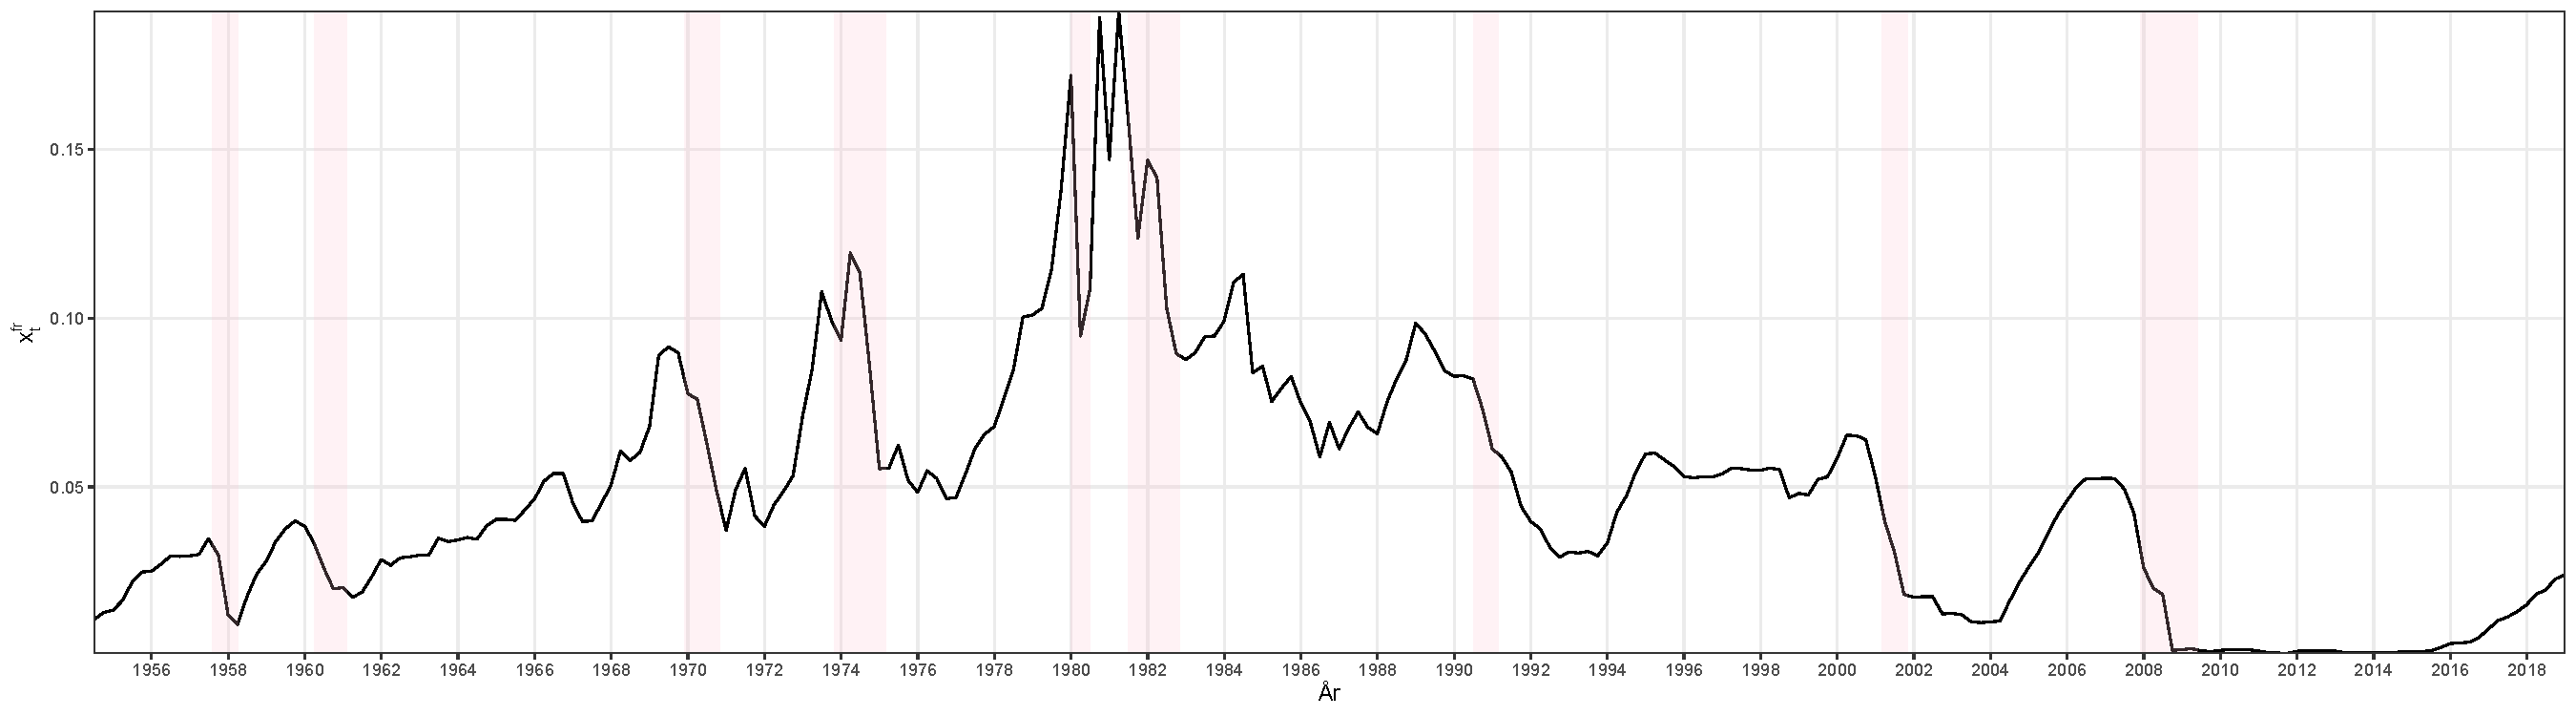
\includegraphics[width=1\linewidth]{Master_Thesis_Andreas_Kracht_Frandsen_files/figure-latex/FR-tids-1} 

}

\caption{Tidsserie af Federal Funds Rate.}\label{fig:FR-tids}
\end{figure}

\begin{figure}[H]

{\centering 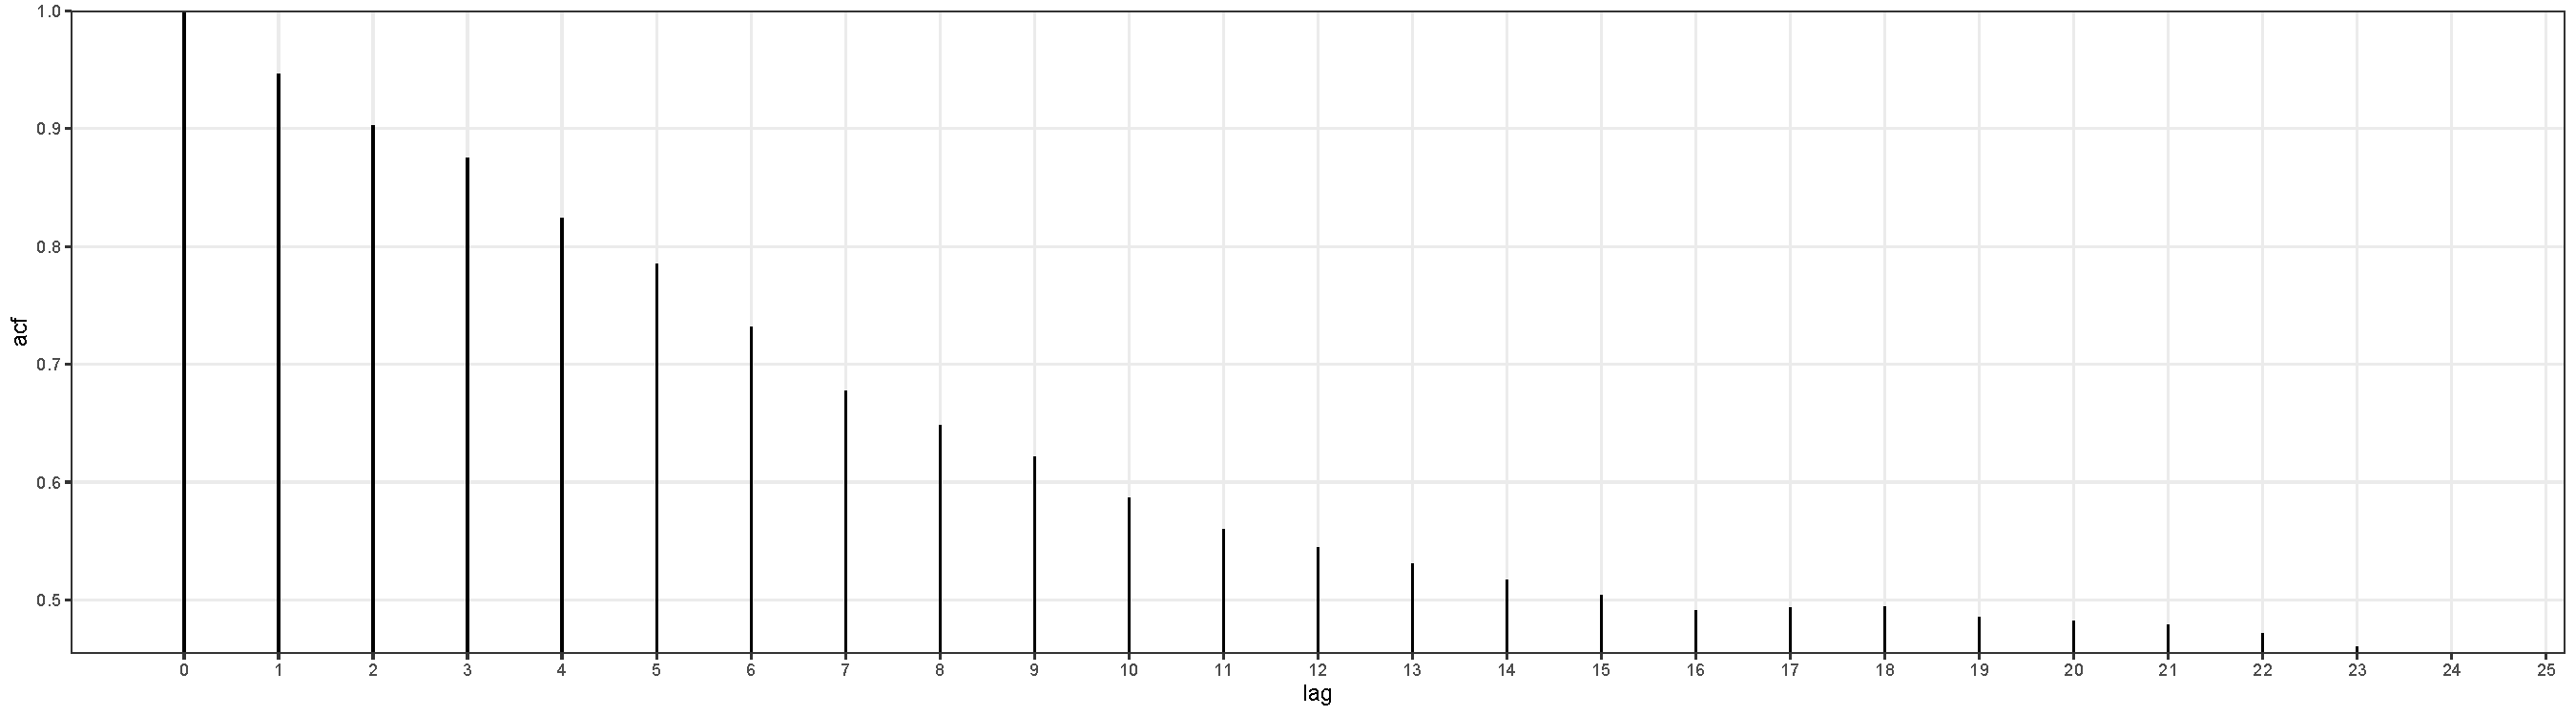
\includegraphics[width=1\linewidth]{Master_Thesis_Andreas_Kracht_Frandsen_files/figure-latex/FR-AK-1} 

}

\caption{Autokorrelation af Federal Funds Rate.}\label{fig:FR-AK}
\end{figure}

\begin{figure}[H]

{\centering \includegraphics[width=1\linewidth]{Master_Thesis_Andreas_Kracht_Frandsen_files/figure-latex/FR-HIST-1} 

}

\caption{Histogram for Federal Funds Rate.}\label{fig:FR-HIST}
\end{figure}

\begin{table}[H]

\caption{\label{tab:DES-TILSTANDSVARIABLE}Beskrivende statistik for prædiktionsvariablene.}
\centering
\resizebox{\linewidth}{!}{
\begin{threeparttable}
\begin{tabular}[t]{lrrrrrrrrrr}
\toprule
  & Middelværdi & Standard afvigelse & Skævhed & Kurtosis & Minimum & $25 \%$ & Median & $75 \%$ & Maksimum & AK(1)\\
\midrule
\rowcolor{gray!6}  $x_t^{\text{dp}}$ & -3.516 & 0.371 & -0.371 & 2.370 & -4.489 & -3.889 & -3.531 & -3.292 & -2.894 & 0.972\\
$x_t^{\text{pe}}$ & 2.754 & 0.407 & 0.958 & 7.520 & 1.716 & 2.421 & 2.704 & 2.882 & 4.697 & 0.934\\
\rowcolor{gray!6}  $x_t^{\text{bm}}$ & 0.505 & 0.248 & 0.771 & 2.981 & 0.125 & 0.314 & 0.483 & 0.645 & 1.202 & 0.977\\
$x_t^{\text{avar}}$ & 0.006 & 0.010 & 7.186 & 68.380 & 0.000 & 0.002 & 0.004 & 0.007 & 0.108 & 0.423\\
\rowcolor{gray!6}  $x_t^{\text{hml}}$ & 0.330 & 1.809 & 0.447 & 4.858 & -6.043 & -0.837 & 0.300 & 1.138 & 8.093 & 0.114\\
$x_t^{\text{smb}}$ & 0.168 & 1.717 & 0.125 & 3.025 & -4.407 & -0.812 & 0.073 & 1.200 & 4.973 & 0.003\\
\rowcolor{gray!6}  $x_t^{\text{b}}$ & 0.012 & 0.008 & 0.903 & 4.313 & 0.000 & 0.006 & 0.011 & 0.016 & 0.042 & 0.922\\
$x_t^{\text{ts}}$ & 0.015 & 0.012 & -0.231 & 3.033 & -0.027 & 0.006 & 0.014 & 0.024 & 0.044 & 0.813\\
\rowcolor{gray!6}  $x_t^{\text{ys}}$ & 0.012 & 0.009 & -0.153 & 3.828 & -0.022 & 0.005 & 0.012 & 0.017 & 0.043 & 0.760\\
$x_t^{\text{cs}}$ & 0.034 & 0.017 & 0.159 & 2.330 & -0.008 & 0.020 & 0.033 & 0.048 & 0.084 & 0.887\\
\rowcolor{gray!6}  $x_t^{\text{ds}}$ & 0.010 & 0.004 & 1.842 & 8.156 & 0.003 & 0.007 & 0.009 & 0.012 & 0.034 & 0.870\\
$x_t^{\text{fr}}$ & 0.048 & 0.036 & 1.053 & 4.625 & 0.001 & 0.021 & 0.045 & 0.065 & 0.191 & 0.946\\
\bottomrule
\end{tabular}
\begin{tablenotes}
\item \textit{Denne tabel rapporterer kvartalsvis beskrivende statistik for prædiktionsvariablene: log Dividend-Price Ratio, log Price-Earnings Ratio, Book-to-Market Ratio, aktievariansen, High Minus Low, Small Minus Big, log afkastet af den nominelle rente, Term Spread, Yield Spread, Credit Spread, Default Spread samt Federal Funds Rate. Dette gøres ud fra $259$ kvartalvise observationer, som spænder over kvartalerne fra 2. kvartal 1954 til 4. kvartal 2018. Middelværdien er justeret for log Dividend-Price ratio, log Earnings-Price Ratio samt log afkastet af den nominelle rente.}
\end{tablenotes}
\end{threeparttable}}
\end{table}

\begin{table}[H]

\caption{\label{tab:JB-TILSTANDSVARIABLE}Jarque-Bera test.}
\centering
\begin{threeparttable}
\begin{tabular}[t]{lrr}
\toprule
  & Teststørrelse & $p$-værdi\\
\midrule
\rowcolor{gray!6}  $x_t^{\text{dp}}$ & 10.204 & 0.006\\
$x_t^{\text{pe}}$ & 260.174 & 0.000\\
\rowcolor{gray!6}  $x_t^{\text{bm}}$ & 25.633 & 0.000\\
$x_t^{\text{avar}}$ & 48357.914 & 0.000\\
\rowcolor{gray!6}  $x_t^{\text{hml}}$ & 45.881 & 0.000\\
$x_t^{\text{smb}}$ & 0.679 & 0.712\\
\rowcolor{gray!6}  $x_t^{\text{b}}$ & 53.814 & 0.000\\
$x_t^{\text{ts}}$ & 2.321 & 0.313\\
\rowcolor{gray!6}  $x_t^{\text{ys}}$ & 8.408 & 0.015\\
$x_t^{\text{cs}}$ & 5.942 & 0.051\\
\rowcolor{gray!6}  $x_t^{\text{ds}}$ & 433.398 & 0.000\\
$x_t^{\text{fr}}$ & 76.362 & 0.000\\
\bottomrule
\end{tabular}
\begin{tablenotes}
\item \textit{Denne tabel rapporterer Jarque-Beta teststørrelser og $p$-værdier for prædiktionsvariablene: log Dividend-Price Ratio, log Price-Earnings Ratio, Book-to-Market Ratio, aktievariansen, High Minus Low, Small Minus Big, log afkastet af den nominelle rente, Term Spread, Yield Spread, Credit Spread, Default Spread samt Federal Funds Rate, \citep{Jarque1980}. Dette gøres ud fra $259$ kvartalvise observationer, som spænder over kvartalerne fra 2. kvartal 1954 til 4. kvartal 2018.}
\end{tablenotes}
\end{threeparttable}
\end{table}

\hypertarget{korr}{%
\section{Korrelation}\label{korr}}

Denne sektion rapporterer korrelationen mellem alle de ovennævnte variable, som inkluderer både aktivklasserne og prædtiktionsvariablene. Korrelation er opsummeret i Tabel \ref{tab:DES-KOR}. En analyse af korrelationen er en vigtig del af datainspektionen, specielt for multivariate processor -- som den introducerede VAR(1)-model fra Sektion \ref{varkapitel} -- når den statistiske sammenhæng mellem flere variable skal uddybes. Ergo for bedre at kunne beskrive, hvordan en variabel påvirker en eller flere andre variabler, analyseres korrelationen på tværs af alle variable.

Fra Tabel \ref{tab:DES-KOR}, ses at alle log merafkast er ikke-negativt korreleret med den risikofrie netto rente. Samtidig bemærkes at korrelationen mellem obligationsmerafkastene er forholdsvis høj. Som forventet er korrelationen med den risikofrie brutto rente højest af alle variable. De finasielle variable har generelt lav korrelation med den risikofrie netto rente, det samme gør sig gældende for rentestruktursvariablene, mens den makroøkonomiske variabel \emph{Federal Funds Rate} har højere korrelation.

Den anden række repræsenterer korrelationen med log merafkastet på aktier. Denne er negativt korreleret med log merafkastet på statsobligationer og positivt korreleret med log merafkastet på virksomhedsobligationer. Mht. prædiktionsvariablene, er den generelt en anelse negativt korreleret med de finansielle variable, mens det samme gør sig gældende for rentestruktursvariablene. Som forventet har aktievariansen en negativ korrelation med log merafkastet på aktier. \emph{Federal Funds Rate} har ligeledes negativ korrelation.

Log merafkastet på statsobligationer er højt korreleret med log merafkastet på virksomhedsobligationer, hvilket indikerer at de har sammenlignelige egenskaber. Mht. de finansielle variable er der generelt en korrelation omkring nul. For rentestruktursvariablene ses en relativt stor positiv korrelation. Dette kunne betyde, at disse har mere statistisk styrke til at prædiktere merafkastet. For makrovariablen ses et højere kontracyklisk mønster end for log merafkastet på aktier.

Den fjerde række svarer til log merafkastet på virksomhedsobligationer. Her ses en blandet korrelation mellem de finansielle variable, mens der generelt ses en positiv korrelation mellem rentestruktursvariablene. Mht. \emph{Federal Funds Rate} ses igen et kontracyklisk mønster, som for resten af serien af log merafkast. Fokuseres nu på prædiktionsvariablene i Tabel \ref{tab:DES-KOR}, er der generelt høj korrelation mellem de finansielle variable, med undtagelse af \emph{Small Minus Big}, \emph{High Minus Low} og aktievariansen. Dette kan være problematisk, da de essentielt kan indeholde samme information, til at prædiktere merafkast. Korrelationskoefficienten mellem de finansielle variable og rentestruktursvariablene er generelt lav. Der ses meget høj korrelation mellem rentespændende. Den makroøkonomiske variabel har et generelt mønster af høj korrelation mellem de andre klasser af prædiktionsvariable.

\begin{table}[H]

\caption{\label{tab:DES-KOR}Korrelationsmatricen mellem alle aktivklasser og prædiktionsvariable.}
\centering
\resizebox{\linewidth}{!}{
\begin{threeparttable}
\begin{tabular}[t]{lrrrrrrrrrrrrrrrr}
\toprule
  & $r_t^{\text{rf}}$ & $rx_t^{\text{a}}$ & $rx_t^{\text{s}}$ & $rx_t^{\text{v}}$ & $x_t^{\text{dp}}$ & $x_t^{\text{pe}}$ & $x_t^{\text{bm}}$ & $x_t^{\text{avar}}$ & $x_t^{\text{hml}}$ & $x_t^{\text{smb}}$ & $x_t^{\text{b}}$ & $x_t^{\text{ts}}$ & $x_t^{\text{ys}}$ & $x_t^{\text{cs}}$ & $x_t^{\text{ds}}$ & $x_t^{\text{fr}}$\\
\midrule
\rowcolor{gray!6}  $r_t^{\text{rf}}$ & 1.00 & 0.00 & 0.32 & 0.34 & 0.14 & -0.06 & 0.06 & 0.21 & 0.02 & -0.07 & 0.43 & 0.01 & 0.11 & 0.01 & 0.20 & 0.29\\
$rx_t^{\text{a}}$ &  & 1.00 & -0.02 & 0.16 & -0.09 & 0.09 & -0.10 & -0.45 & -0.26 & 0.41 & -0.13 & 0.07 & 0.07 & -0.04 & -0.22 & -0.11\\
\rowcolor{gray!6}  $rx_t^{\text{s}}$ &  &  & 1.00 & 0.85 & -0.05 & 0.06 & -0.07 & 0.26 & -0.01 & -0.10 & 0.03 & 0.19 & 0.13 & 0.26 & 0.12 & -0.18\\
$rx_t^{\text{v}}$ &  &  &  & 1.00 & -0.09 & 0.14 & -0.11 & 0.24 & -0.01 & -0.05 & -0.05 & 0.24 & 0.18 & 0.26 & 0.04 & -0.23\\
\rowcolor{gray!6}  $x_t^{\text{dp}}$ &  &  &  &  & 1.00 & -0.71 & 0.88 & -0.06 & 0.04 & 0.00 & 0.50 & -0.09 & 0.03 & -0.21 & 0.28 & 0.48\\
$x_t^{\text{pe}}$ &  &  &  &  &  & 1.00 & -0.77 & 0.27 & -0.09 & 0.04 & -0.56 & 0.29 & 0.19 & 0.35 & -0.15 & -0.57\\
\rowcolor{gray!6}  $x_t^{\text{bm}}$ &  &  &  &  &  &  & 1.00 & -0.08 & 0.08 & 0.06 & 0.61 & -0.13 & -0.01 & -0.17 & 0.40 & 0.61\\
$x_t^{\text{avar}}$ &  &  &  &  &  &  &  & 1.00 & -0.09 & -0.13 & -0.04 & 0.16 & 0.10 & 0.35 & 0.42 & -0.09\\
\rowcolor{gray!6}  $x_t^{\text{hml}}$ &  &  &  &  &  &  &  &  & 1.00 & -0.10 & 0.09 & 0.06 & 0.07 & 0.02 & -0.03 & 0.06\\
$x_t^{\text{smb}}$ &  &  &  &  &  &  &  &  &  & 1.00 & -0.03 & 0.07 & 0.10 & 0.05 & 0.01 & 0.01\\
\rowcolor{gray!6}  $x_t^{\text{b}}$ &  &  &  &  &  &  &  &  &  &  & 1.00 & -0.20 & -0.03 & -0.16 & 0.42 & 0.90\\
$x_t^{\text{ts}}$ &  &  &  &  &  &  &  &  &  &  &  & 1.00 & 0.96 & 0.90 & 0.27 & -0.41\\
\rowcolor{gray!6}  $x_t^{\text{ys}}$ &  &  &  &  &  &  &  &  &  &  &  &  & 1.00 & 0.81 & 0.27 & -0.25\\
$x_t^{\text{cs}}$ &  &  &  &  &  &  &  &  &  &  &  &  &  & 1.00 & 0.53 & -0.36\\
\rowcolor{gray!6}  $x_t^{\text{ds}}$ &  &  &  &  &  &  &  &  &  &  &  &  &  &  & 1.00 & 0.32\\
$x_t^{\text{fr}}$ &  &  &  &  &  &  &  &  &  &  &  &  &  &  &  & 1.00\\
\bottomrule
\end{tabular}
\begin{tablenotes}
\item \textit{Denne tabel rapporterer korrelationsmatricen i øvre triangulær form mellem alle beskrevne variable: det risikofrie aktiv, merafkastet på aktier, merafkastet på statsobligationer, merafkastet på virksomhedsobligationer, log Dividend-Price Ratio, log Price-Earnings Ratio, Book-to-Market Ratio, aktievariansen, High Minus Low, Small Minus Big, log afkastet af den nominelle rente, Term Spread, Yield Spread, Credit Spread, Default Spread samt Federal Funds Rate. Dette gøres ud fra $259$ kvartalvise observationer, som spænder over kvartalerne fra 2. kvartal 1954 til 4. kvartal 2018.}
\end{tablenotes}
\end{threeparttable}}
\end{table}

\hypertarget{stationar}{%
\section{Stationaritet}\label{stationar}}

Som nævnt tidligere er stationaritet af de anvendte tidsserier et bærende element for validiteten af den endelige VAR(1)-model. I denne sektion vil en række testprocedure blive udført, for at kontrollere for stationaritet, på en mere formel måde end visuel inspektion. Tre forskellige test vil tilsammen skabe et grundlag for at afgøre om en eller flere af alle tilstandsvariablene skal ekskluderes fra den endelige VAR(1)-model. Disse er hhv. \emph{Augmented Dickey-Fuller} test, \emph{Phillips-Perron} test samt \emph{Kwiatkowski-Phillips-Schmidt-Shin}.

\hypertarget{augdickful}{%
\subsection{Augmented Dickey-Fuller Test}\label{augdickful}}

\emph{Augmented Dickey-Fuller} test outputtet ses i Tabel \ref{tab:STAT}. Først og fremmest ses, at vi afvise hypotesen om ikke-stationaritet hos alle aktivklasserne -- på et signifikansniveau på \(\alpha=0.05\) -- når fokus er på de første par lags. Dette var også forventet givet en inspektion af de relevante tidsserie plots. Fokuseres dernæst på prædiktionsvariablene er det kun \emph{Dividend-Price Ratio}, \emph{Book-to-Market Ratio}, den nominelle rente samt \emph{Federal Funds Rate}, som ikke kan forkaste hypotesen om ikke-stationaritet. \emph{Price-Earnings} kan kun forkaste hypotesen for et signifikansniveau på \(\alpha=0.1\), uden lags. Hvorimod resten af prædiktionsvariablene forkaster hypotesen for alle lags. For at verificere, at de tre nævnte ovennævnte variable potentielt er eksplosive eller har en \emph{unit root}, tages den første forskel på tidsserierne. Herefter foretages testen igen. Outputtet fra denne re-testning ses i Tabel \ref{tab:STAT-DIFF}. Som det kan aflæses i tabellen er alle variablene integreret af første orden, \(I(1)\), eller stationære med hensyn til deres første forskel.

Håndteringen af potentielle ikke-stationære tidsserier er mere problematisk. Essentielt kan de problematiske variable udelades fra resten af analysen. På den anden side vil afvisning af de såkaldte \emph{difference stationary} serier være ufornuftigt, da disse ikke kan skabe problemer for den færdige model. Den generelle statistiske metode, ville være at fortsætte analysen med brug af disse nye serier: \(x_t^{\text{dp}_{\Delta}}\), \(x_t^{\text{bm}_{\Delta}}\), \(x_t^{\text{b}_{\Delta}}\) og \(x_t^{\text{fr}_{\Delta}}\). Men flere argumenter taler til gengæld imod denne procedure. Først og fremmest er det generelt accepteret i litteraturen at anvende disse variable i niveauer. For det andet vil mange variable miste deres intuitive prædiktionskvaliteter, da deres niveau er en del af argumentationen for at medtage dem. For det tredje vides det fra økonomisk intuition, at disse variable ikke kan blive eksplosive af konstruktion.






\begin{table}[H]

\caption{\label{tab:STAT}Augmented Dickey-Fuller.}
\centering
\resizebox{\linewidth}{!}{
\begin{threeparttable}
\begin{tabular}[t]{lrrrrrrrrrrrr}
\toprule
\multicolumn{1}{c}{ } & \multicolumn{2}{c}{$\delta=0$} & \multicolumn{2}{c}{$\delta=1$} & \multicolumn{2}{c}{$\delta=2$} & \multicolumn{2}{c}{$\delta=3$} & \multicolumn{2}{c}{$\delta=4$} & \multicolumn{2}{c}{$\delta^*=5$} \\
\cmidrule(l{3pt}r{3pt}){2-3} \cmidrule(l{3pt}r{3pt}){4-5} \cmidrule(l{3pt}r{3pt}){6-7} \cmidrule(l{3pt}r{3pt}){8-9} \cmidrule(l{3pt}r{3pt}){10-11} \cmidrule(l{3pt}r{3pt}){12-13}
  & Teststørrelse & $p$-værdi & Teststørrelse & $p$-værdi & Teststørrelse & $p$-værdi & Teststørrelse & $p$-værdi & Teststørrelse & $p$-værdi & Teststørrelse & $p$-værdi\\
\midrule
\rowcolor{gray!6}  $r_t^{\text{rf}}$ & -11.629 & 0.010 & -8.085 & 0.010 & -5.597 & 0.010 & -3.219 & 0.085 & -3.031 & 0.142 & -3.087 & 0.118\\
$rx_t^{\text{a}}$ & -14.689 & 0.010 & -11.556 & 0.010 & -9.732 & 0.010 & -8.465 & 0.010 & -7.542 & 0.010 & -7.115 & 0.010\\
\rowcolor{gray!6}  $rx_t^{\text{s}}$ & -16.076 & 0.010 & -12.079 & 0.010 & -8.889 & 0.010 & -7.598 & 0.010 & -8.364 & 0.010 & -7.580 & 0.010\\
$rx_t^{\text{v}}$ & -17.174 & 0.010 & -11.531 & 0.010 & -8.553 & 0.010 & -7.471 & 0.010 & -7.307 & 0.010 & -6.846 & 0.010\\
\rowcolor{gray!6}  $x_t^{\text{dp}}$ & -2.285 & 0.456 & -2.446 & 0.388 & -2.241 & 0.474 & -2.123 & 0.524 & -2.090 & 0.538 & -2.055 & 0.553\\
$x_t^{\text{pe}}$ & -3.270 & 0.077 & -4.675 & 0.010 & -4.545 & 0.010 & -3.620 & 0.032 & -3.189 & 0.090 & -3.555 & 0.038\\
\rowcolor{gray!6}  $x_t^{\text{bm}}$ & -1.933 & 0.604 & -2.220 & 0.483 & -2.173 & 0.503 & -2.046 & 0.557 & -2.073 & 0.545 & -1.896 & 0.620\\
$x_t^{\text{avar}}$ & -10.476 & 0.010 & -8.685 & 0.010 & -7.350 & 0.010 & -6.670 & 0.010 & -5.898 & 0.010 & -5.490 & 0.010\\
\rowcolor{gray!6}  $x_t^{\text{hml}}$ & -14.316 & 0.010 & -10.675 & 0.010 & -9.137 & 0.010 & -7.820 & 0.010 & -7.655 & 0.010 & -6.568 & 0.010\\
$x_t^{\text{smb}}$ & -15.855 & 0.010 & -10.072 & 0.010 & -8.590 & 0.010 & -6.413 & 0.010 & -6.087 & 0.010 & -5.751 & 0.010\\
\rowcolor{gray!6}  $x_t^{\text{b}}$ & -3.525 & 0.041 & -2.741 & 0.264 & -2.350 & 0.429 & -2.517 & 0.358 & -2.687 & 0.287 & -2.773 & 0.250\\
$x_t^{\text{ts}}$ & -5.285 & 0.010 & -4.946 & 0.010 & -4.022 & 0.010 & -5.036 & 0.010 & -4.502 & 0.010 & -5.266 & 0.010\\
\rowcolor{gray!6}  $x_t^{\text{ys}}$ & -5.840 & 0.010 & -5.449 & 0.010 & -4.319 & 0.010 & -5.076 & 0.010 & -4.749 & 0.010 & -5.284 & 0.010\\
$x_t^{\text{cs}}$ & -4.519 & 0.010 & -4.490 & 0.010 & -3.856 & 0.017 & -5.020 & 0.010 & -4.670 & 0.010 & -5.265 & 0.010\\
\rowcolor{gray!6}  $x_t^{\text{ds}}$ & -4.293 & 0.010 & -4.622 & 0.010 & -4.142 & 0.010 & -4.042 & 0.010 & -3.983 & 0.010 & -3.511 & 0.042\\
$x_t^{\text{fr}}$ & -2.951 & 0.175 & -2.734 & 0.267 & -2.408 & 0.404 & -2.844 & 0.221 & -2.592 & 0.327 & -3.131 & 0.100\\
\bottomrule
\end{tabular}
\begin{tablenotes}
\item \textit{Denne tabel rapporterer Augmented Dickey-Fuller teststørrelser og $p$-værdier for alle beskrevne variable: det risikofrie aktiv, merafkastet på aktier, merafkastet på statsobligationer, merafkastet på virksomhedsobligationer, log Dividend-Price Ratio, log Price-Earnings Ratio, Book-to-Market Ratio, aktievariansen, High Minus Low, Small Minus Big, log afkastet af den nominelle rente, Term Spread, Yield Spread, Credit Spread, Default Spread samt Federal Funds Rate, \citep{Dickey1979}. Testen er udført for forskellige lags, samt et lag, $\delta^*$, fastsat til heltalsdelen af $4(T/100)^{1/4}$ -- som foreslået af \citep{Schwert1989} -- hvor $T=259$. Dette gøres ud fra $259$ kvartalvise observationer, som spænder over kvartalerne fra 2. kvartal 1954 til 4. kvartal 2018.}
\end{tablenotes}
\end{threeparttable}}
\end{table}

\begin{table}[H]

\caption{\label{tab:STAT-DIFF}Augmented Dickey-Fuller. For første forskelle.}
\centering
\resizebox{\linewidth}{!}{
\begin{threeparttable}
\begin{tabular}[t]{lrrrrrrrrrrrr}
\toprule
\multicolumn{1}{c}{ } & \multicolumn{2}{c}{$\delta=0$} & \multicolumn{2}{c}{$\delta=1$} & \multicolumn{2}{c}{$\delta=2$} & \multicolumn{2}{c}{$\delta=3$} & \multicolumn{2}{c}{$\delta=4$} & \multicolumn{2}{c}{$\delta^*=5$} \\
\cmidrule(l{3pt}r{3pt}){2-3} \cmidrule(l{3pt}r{3pt}){4-5} \cmidrule(l{3pt}r{3pt}){6-7} \cmidrule(l{3pt}r{3pt}){8-9} \cmidrule(l{3pt}r{3pt}){10-11} \cmidrule(l{3pt}r{3pt}){12-13}
  & Teststørrelse & $p$-værdi & Teststørrelse & $p$-værdi & Teststørrelse & $p$-værdi & Teststørrelse & $p$-værdi & Teststørrelse & $p$-værdi & Teststørrelse & $p$-værdi\\
\midrule
\rowcolor{gray!6}  $x_t^{\text{dp}_{\Delta}}$ & -14.798 & 0.010 & -11.778 & 0.010 & -9.962 & 0.010 & -8.575 & 0.010 & -7.649 & 0.010 & -7.403 & 0.010\\
$x_t^{\text{bm}_{\Delta}}$ & -14.054 & 0.010 & -11.046 & 0.010 & -9.595 & 0.010 & -8.386 & 0.010 & -8.206 & 0.010 & -8.089 & 0.010\\
\rowcolor{gray!6}  $x_t^{\text{b}_{\Delta}}$ & -22.282 & 0.010 & -15.975 & 0.010 & -10.397 & 0.010 & -7.799 & 0.010 & -6.783 & 0.010 & -5.700 & 0.010\\
$x_t^{\text{fr}_{\Delta}}$ & -17.626 & 0.010 & -14.010 & 0.010 & -8.495 & 0.010 & -8.297 & 0.010 & -5.878 & 0.010 & -5.913 & 0.010\\
\bottomrule
\end{tabular}
\begin{tablenotes}
\item \textit{Denne tabel rapporterer Augmented Dickey-Fuller teststørrelser og $p$-værdier for 'first-difference'-variablene: log Dividend-Price Ratio, Book-to-Market Ratio, log afkastet af den nominelle rente samt Federal Funds Rate, \citep{Dickey1979}. Testen er udført for forskellige lags, samt et lag, $\delta^*$, fastsat til heltalsdelen af $4(T/100)^{1/4}$ -- som foreslået af \citep{Schwert1989} -- hvor $T=259$. Dette gøres ud fra $259$ kvartalvise observationer, som spænder over kvartalerne fra 2. kvartal 1954 til 4. kvartal 2018.}
\end{tablenotes}
\end{threeparttable}}
\end{table}

\hypertarget{philper}{%
\subsection{Phillips-Perron test}\label{philper}}

Som en validering af resultaterne fra \emph{Augmented Dickey Fuller} test, foretages \emph{Phillips-Perron} testen. Outputtet fra denne ses i Tabel \ref{tab:STAT-PP}. Igen er det \emph{Dividend-Price Ratio}, \emph{Book-to-Market Ratio}, den nominelle rente samt \emph{Federal Funds Rate}, som er problematiske.

\begin{table}[H]

\caption{\label{tab:STAT-PP}Phillips-Perron Test.}
\centering
\begin{threeparttable}
\begin{tabular}[t]{lrrrr}
\toprule
\multicolumn{1}{c}{ } & \multicolumn{4}{c}{$l=5$} \\
\cmidrule(l{3pt}r{3pt}){2-5}
\multicolumn{1}{c}{ } & \multicolumn{2}{c}{$Z(\hat{\alpha})$} & \multicolumn{2}{c}{$Z(t_{\hat{\alpha}})$} \\
\cmidrule(l{3pt}r{3pt}){2-3} \cmidrule(l{3pt}r{3pt}){4-5}
  & Teststørrelse & $p$-værdi & Teststørrelse & $p$-værdi\\
\midrule
\rowcolor{gray!6}  $r_t^{\text{rf}}$ & -233.688 & 0.010 & -12.546 & 0.010\\
$rx_t^{\text{a}}$ & -220.300 & 0.010 & -14.622 & 0.010\\
\rowcolor{gray!6}  $rx_t^{\text{s}}$ & -250.336 & 0.010 & -16.088 & 0.010\\
$rx_t^{\text{v}}$ & -285.340 & 0.010 & -17.145 & 0.010\\
\rowcolor{gray!6}  $x_t^{\text{dp}}$ & -10.744 & 0.507 & -2.301 & 0.449\\
$x_t^{\text{pe}}$ & -26.987 & 0.015 & -3.700 & 0.024\\
\rowcolor{gray!6}  $x_t^{\text{bm}}$ & -8.338 & 0.642 & -2.045 & 0.557\\
$x_t^{\text{avar}}$ & -157.735 & 0.010 & -10.522 & 0.010\\
\rowcolor{gray!6}  $x_t^{\text{hml}}$ & -223.350 & 0.010 & -14.277 & 0.010\\
$x_t^{\text{smb}}$ & -285.632 & 0.010 & -15.960 & 0.010\\
\rowcolor{gray!6}  $x_t^{\text{b}}$ & -16.685 & 0.174 & -3.088 & 0.118\\
$x_t^{\text{ts}}$ & -55.607 & 0.010 & -5.436 & 0.010\\
\rowcolor{gray!6}  $x_t^{\text{ys}}$ & -64.954 & 0.010 & -5.958 & 0.010\\
$x_t^{\text{cs}}$ & -45.693 & 0.010 & -4.839 & 0.010\\
\rowcolor{gray!6}  $x_t^{\text{ds}}$ & -35.018 & 0.010 & -4.317 & 0.010\\
$x_t^{\text{fr}}$ & -14.944 & 0.272 & -2.895 & 0.199\\
\bottomrule
\end{tabular}
\begin{tablenotes}
\item \textit{Denne tabel rapporterer Phillips-Perron teststørrelser og $p$-værdier for alle beskrevne variable: det risikofrie aktiv, merafkastet på aktier, merafkastet på statsobligationer, merafkastet på virksomhedsobligationer, log Dividend-Price Ratio, log Price-Earnings Ratio, Book-to-Market Ratio, aktievariansen, High Minus Low, Small Minus Big, log afkastet af den nominelle rente, Term Spread, Yield Spread, Credit Spread, Default Spread samt Federal Funds Rate, \citep{Phillips1988}. Dette gøres ud fra $259$ kvartalvise observationer, som spænder over kvartalerne fra 2. kvartal 1954 til 4. kvartal 2018. Testen er udført for et lag fastsat til heltalsdelen af $4(T/100)^{1/4}$ -- som foreslået af \citep{Schwert1989} -- hvor $T=259$.}
\end{tablenotes}
\end{threeparttable}
\end{table}

\hypertarget{kwiatkow}{%
\subsection{Kwiatkowski-Phillips-Schmidt-Shin test}\label{kwiatkow}}

Som en ekstra validering foretages \emph{Kwiatkowski-Phillips-Schmidt-Shin} testen. Nulhypotesen er i dette tilfælde omvendt. Outputtet fra testen ses i Tabel \ref{tab:STAT-KPSS}. Det ses, at \emph{KPSS} testen modsiger resultaterne fra både \emph{Augmented Dickey-Fuller} testen og \emph{Phillips-Perron} testen, for visse variable. Dette er imidlertid et kendt problem, som generelt opstår grundet en begrænset stikprøvestørrelse.

\begin{table}[H]

\caption{\label{tab:STAT-KPSS}Kwiatkowski-Phillips-Schmidt-Shin Test.}
\centering
\begin{threeparttable}
\begin{tabular}[t]{lrrrr}
\toprule
\multicolumn{1}{c}{ } & \multicolumn{4}{c}{$l=5$} \\
\cmidrule(l{3pt}r{3pt}){2-5}
\multicolumn{1}{c}{ } & \multicolumn{2}{c}{Level} & \multicolumn{2}{c}{Trend} \\
\cmidrule(l{3pt}r{3pt}){2-3} \cmidrule(l{3pt}r{3pt}){4-5}
  & Teststørrelse (LM) & $p$-værdi & Teststørrelse (LM) & $p$-værdi\\
\midrule
\rowcolor{gray!6}  $r_t^{\text{rf}}$ & 0.500 & 0.042 & 0.334 & 0.010\\
$rx_t^{\text{a}}$ & 0.059 & 0.100 & 0.060 & 0.100\\
\rowcolor{gray!6}  $rx_t^{\text{s}}$ & 0.469 & 0.049 & 0.039 & 0.100\\
$rx_t^{\text{v}}$ & 0.581 & 0.024 & 0.037 & 0.100\\
\rowcolor{gray!6}  $x_t^{\text{dp}}$ & 2.448 & 0.010 & 0.397 & 0.010\\
$x_t^{\text{pe}}$ & 1.526 & 0.010 & 0.326 & 0.010\\
\rowcolor{gray!6}  $x_t^{\text{bm}}$ & 2.102 & 0.010 & 0.501 & 0.010\\
$x_t^{\text{avar}}$ & 0.626 & 0.020 & 0.046 & 0.100\\
\rowcolor{gray!6}  $x_t^{\text{hml}}$ & 0.185 & 0.100 & 0.052 & 0.100\\
$x_t^{\text{smb}}$ & 0.063 & 0.100 & 0.051 & 0.100\\
\rowcolor{gray!6}  $x_t^{\text{b}}$ & 1.191 & 0.010 & 0.794 & 0.010\\
$x_t^{\text{ts}}$ & 0.753 & 0.010 & 0.071 & 0.100\\
\rowcolor{gray!6}  $x_t^{\text{ys}}$ & 0.331 & 0.100 & 0.132 & 0.075\\
$x_t^{\text{cs}}$ & 1.671 & 0.010 & 0.079 & 0.100\\
\rowcolor{gray!6}  $x_t^{\text{ds}}$ & 0.451 & 0.055 & 0.297 & 0.010\\
$x_t^{\text{fr}}$ & 1.155 & 0.010 & 0.754 & 0.010\\
\bottomrule
\end{tabular}
\begin{tablenotes}
\item \textit{Denne tabel rapporterer Kwiatkowski-Phillips-Schmidt-Shin teststørrelser og $p$-værdier for alle beskrevne variable: det risikofrie aktiv, merafkastet på aktier, merafkastet på statsobligationer, merafkastet på virksomhedsobligationer, log Dividend-Price Ratio, log Price-Earnings Ratio, Book-to-Market Ratio, aktievariansen, High Minus Low, Small Minus Big, log afkastet af den nominelle rente, Term Spread, Yield Spread, Credit Spread, Default Spread samt Federal Funds Rate, \citep{Kwiatkowski1992}. Dette gøres ud fra $259$ kvartalvise observationer, som spænder over kvartalerne fra 2. kvartal 1954 til 4. kvartal 2018. Testen er udført for et lag fastsat til heltalsdelen af $4(T/100)^{1/4}$ -- som foreslået af \citep{Schwert1989} -- hvor $T=259$.}
\end{tablenotes}
\end{threeparttable}
\end{table}

\hypertarget{ops}{%
\section{Opsummering}\label{ops}}

Dette kapitel fungerede som en detaljeret data beskrivelse af alle undersøgte variable inkluderet til den videre analyse. Kapitlet indeholdte både beskrivende statistik samt plots og derudover beregninger og estimationsprocedure. Inspektion af autokorrelation i hver variabel viste, at log merafkastene ikke er udsat for autokorrelation, mens det risikofrie afkast udviser en smule autokorrelation. Derimod viste stort set alle prædiktionsvariable høj autokorrelation som generelt næsten var lig \(1\). Dette betyder at de generelt er meget vedvarende over tid. Dette kunne blive et problem for den videre analyse, idet, at de potentielt kan medfører bias pga. den endelige stikprøvestørrelse. En kvantitativ og kvalitativ vurdering af normaliteten af alle variable indebar, at næsten alle variable ikke udviser normalitet, dette kan tilgengæld være påvirket af stikprøvestørrelsen. Korrelationer blandt alle variable, følger generelt andre fund i eksisterende litteratur. Sidst foretog kapitlet en analyse af den mulige stationaritet blandt alle variable.

\hypertarget{predikta}{%
\chapter{Prædiktabilitet}\label{predikta}}

Dette kapitel har til formål at teste for prædiktabilitet af afkastene i de introducerede aktivklasser fra Sektion \ref{aktivklasser}, ved benyttelse af de introducerede mulige prædiktionsvariable fra Sektion \ref{pvariable}. Prædiktabiliteten bliver testet i både et univariat og et multipelt øjemed. Dette tillader at teste for robusthed på tværs af prædiktionsvariablene og drage inferens af den mulige linearitet imellem merafkastene på aktivklasserne og de forklarende variable. Derudover vil testene giver et fingerpeg om graden af variationsforklaring, som de individuelle prædiktionsvariable måtte have, ift. responsvariablene. Disse regressioner vil have til formål at bidrage til delmængden af variable, som senere skal indgå i variabeludvælgelsen for VAR(1)-modellen. Det primære fokus vil være på de fundamentale variable, som før har vist særlig prædiktabilitets evner. Sekundært vil koefficienter, fortegn samt signifikans for hver individuel variabel blive beskrevet.

Kapitlets opbygning er som følger: Sektion \ref{unireg} beskriver og diskuterer de univariate regressioner, Sektion \ref{multreg} beskriver og diskuterer de multiple regressioner sidst vil Sektion \ref{opsreg} en opsummering af kapitlets fund.

\hypertarget{unireg}{%
\section{Univariate regressioner}\label{unireg}}

Denne sektion rapporterer de univariate regressioner af responsvariable fra Sektion \ref{aktivklasser} på sættet af prædiktionsvariable fra Sektion \ref{pvariable}. Afskæringer bliver ikke rapporteret, eftersom det kun er den mulige prædiktabilitets evne, som har interesse for analysen. Standardfejl er justeret for heteroskedasticitet og autokorrelation, \citep{Newey1987}. \(t\)-værdierne og \(p\)-værdierne er ligedes dannet på baggrund af de justerede standardfejl. Signifikansniveauet fastholdes på niveauet \(\alpha=0.05\).

Den univariate analyse består af følgende regressioner
\[rx_{t+1}^j=\beta_{0}^i+\beta_{1}^ix_{t}^i+\varepsilon_{t+1}^i,\]

hvor \(j\) er notationen for de \(3\) aktivklasser bestående af merafkast og \(i\) er notationen for de \(12\) prædiktionsvariable. Den statistiske signifikans for hver individuel koefficient vil kort blive vurderet, da dette vil give et fingerpeg om den mulige styrke, for hver forklarende variabel ift. prædiktion af fremtidige afkast. Mest opmærksomhed vil dog stadig være på aktivklassernes fundamentale relation til visse variable.

Tabel \ref{tab:UNI-ak} rapporterer de univariate regressions resultater af merafkastet på aktier, \(rx_{t+1}^a\), overfor den introducerede delmængde af mulige prædiktionsvariable. Det kendte nøgletal \emph{Dividend-Price Ratio} er ikke signifikant for hverken et \(5\%\) eller \(10\%\) signifikansniveau, med en tilhørende \(t\)-størrelse på 1.606. Af de resterende finansielle variable er det \emph{Price-Earnings Ratio}, \emph{Book-to-Market Ratio}, \emph{High Minus Low} og \emph{Small Minus Big} som prædiktrer merafkastet på aktier negativt. Af disse er det kun \emph{Small Minus Big} som påviser signifikans, med en \(t\)-størrelse på -2.671. Fortegnene for de finansielle variable er ækvivalente med tidligere i fund i litteraturen, eksempelvis \citep{Camp1987} og \citep{CampVicCha2003}. Den sidste signifikante variabel er \emph{Term-Spread} med \(t\)-størrelse på 2.152. På et \(10\%\) signifikansniveau vil også \emph{Yield Spread} være statistisk signifikant, og kunne derfor også være en mulig variabel til prædiktion af merafkastet på aktier. Størstedelen af rentestrukturs variablene prædikterer merafkastet positivt, med undtagelse af den nominelle rente og \emph{Default Spread}. Hvilket for rentespændende er ensbetydende med, at når spændet mellem langsigtede instrumenter og kortsigtede instrumenter stiger, vil en øgning i merafkastet på aktier, \(rx_{t+1}^s\), ligeledes ske i den næstkommende periode.



\begin{table}[H]

\caption{\label{tab:UNI-ak}Univariat prædiktabilitet af merafkastet på aktier.}
\centering
\begin{threeparttable}
\begin{tabular}[t]{lrrrrrrr}
\toprule
\multicolumn{1}{c}{$rx_{t+1}^{\text{a}}$} & \multicolumn{1}{c}{ } & \multicolumn{2}{c}{Konfidensinterval} & \multicolumn{4}{c}{ } \\
\cmidrule(l{3pt}r{3pt}){1-1} \cmidrule(l{3pt}r{3pt}){3-4}
  & Koefficient & Nedre & Øvre & Standardfejl & $t$-værdi & $p$ & $R^2$\\
\midrule
\rowcolor{gray!6}  $x_t^{\text{dp}}$ & 0.024 & -0.005 & 0.054 & 0.015 & 1.606 & 0.110 & 0.011\\
$x_t^{\text{pe}}$ & -0.009 & -0.044 & 0.027 & 0.018 & -0.480 & 0.631 & 0.002\\
\rowcolor{gray!6}  $x_t^{\text{bm}}$ & 0.016 & -0.024 & 0.056 & 0.020 & 0.779 & 0.437 & 0.002\\
$x_t^{\sigma_{\text{a}}^2}$ & 0.278 & -1.317 & 1.873 & 0.810 & 0.343 & 0.732 & 0.001\\
\rowcolor{gray!6}  $x_t^{\text{hml}}$ & -0.004 & -0.009 & 0.001 & 0.003 & -1.496 & 0.136 & 0.007\\
$x_t^{\text{smb}}$ & \textbf{-0.006} & -0.010 & -0.002 & 0.002 & -2.671 & 0.008 & 0.015\\
\rowcolor{gray!6}  $x_t^{\text{b}}$ & -0.850 & -2.110 & 0.410 & 0.640 & -1.328 & 0.185 & 0.007\\
$x_t^{\text{ts}}$ & \textbf{ 0.976} & 0.083 & 1.870 & 0.454 & 2.152 & 0.032 & 0.019\\
\rowcolor{gray!6}  $x_t^{\text{ys}}$ & 1.014 & -0.035 & 2.062 & 0.532 & 1.904 & 0.058 & 0.013\\
$x_t^{\text{cs}}$ & 0.312 & -0.502 & 1.126 & 0.413 & 0.755 & 0.451 & 0.004\\
\rowcolor{gray!6}  $x_t^{\text{ds}}$ & -1.049 & -5.042 & 2.944 & 2.028 & -0.517 & 0.605 & 0.003\\
$x_t^{\text{fr}}$ & \textbf{-0.386} & -0.697 & -0.075 & 0.158 & -2.445 & 0.015 & 0.028\\
\bottomrule
\end{tabular}
\begin{tablenotes}
\item \textit{Denne tabel rapporterer den beskrivende statistik af de univariate regressioner ift. responsvariablen: merafkastet på aktier, $rx_{t+1}^{\text{a}}$. Hver række svarer til én selvstændig regression. Dette gøres ud fra $259$ kvartalvise observationer, som spænder over kvartalerne fra 2. kvartal 1954 til 4. kvartal 2018. Koefficienter markeret med \textbf{fed} implicerer signifikans, for et signifikansniveau på $\alpha=0.05$. Standardfejl er justeret for heteroskedasticitet og autokorrelation, \citep{Newey1987}. Konfidensintervallerne for koefficienterne, $t$-værdierne og $p$-værdierne er ligedes dannet på baggrund af de justerede standardfejl. $R^2$ er ligedes rapporteret, bemærk dette ikke er den justerede $R^2$.}
\end{tablenotes}
\end{threeparttable}
\end{table}

Ligedes rapporterer Tabel \ref{tab:UNI-s} de univariate regressions resultater af merafkastet på statsobligationer, \(rx_{t+1}^s\), overfor den introducerede delmængde af mulige prædiktionsvariable. Mest overraskende er, at \emph{Yield Spread} ikke er signifikant, som den eneste af de fire rentespænds variable. Til gengæld prædikterer \emph{Yield Spread} merafkastet på statsobligationer positivt, hvilket også følger tidligere litteratur, \citep{Fama1987}. Dette er også tilfældet for de resterende rentespænd. Af alle rentestruktursvariablene er det kun \emph{Term Spread}, \emph{Credit Spread} og \emph{Default Spread} som er signifikante for denne stikprøve, med \(t\)-størrelser på hhv. 2.466, 4.297 og 2.858. En stigning i den nuværende \emph{Term Spread} kommer eksempelvis enten fra en forøgelse af den lange effektive rente, \(Y_t^{10}\), eller et fald i den korte effektive rente, \(Y_t^90\), eller en kombination af begge vil lede til en stigning i det fremtidige log merafkast på statsobligationer. Ift. de finansielle variable er det \emph{Small Minus Big}, som har statistisk styrke i den univariate opsætning, med \(t\)-størrelse på -2.702. \emph{Small Minus Big} prædikterer merafkastet negativt. Den makroøkonomiske variabel \emph{Federal Funds Rate} er ikke signifikant, og prædikterer merafkastet negativt.

\begin{table}[H]

\caption{\label{tab:UNI-s}Univariat prædiktabilitet af merafkastet på statsobligationer.}
\centering
\begin{threeparttable}
\begin{tabular}[t]{lrrrrrrr}
\toprule
\multicolumn{1}{c}{$rx_{t+1}^{\text{s}}$} & \multicolumn{1}{c}{ } & \multicolumn{2}{c}{Konfidensinterval} & \multicolumn{4}{c}{ } \\
\cmidrule(l{3pt}r{3pt}){1-1} \cmidrule(l{3pt}r{3pt}){3-4}
  & Koefficient & Nedre & Øvre & Standardfejl & $t$-værdi & $p$ & $R^2$\\
\midrule
\rowcolor{gray!6}  $x_t^{\text{dp}}$ & -0.006 & -0.019 & 0.008 & 0.007 & -0.852 & 0.395 & 0.003\\
$x_t^{\text{pe}}$ & 0.001 & -0.010 & 0.013 & 0.006 & 0.196 & 0.845 & 0.000\\
\rowcolor{gray!6}  $x_t^{\text{bm}}$ & -0.007 & -0.030 & 0.017 & 0.012 & -0.545 & 0.586 & 0.002\\
$x_t^{\sigma_{\text{a}}^2}$ & 0.107 & -0.178 & 0.391 & 0.145 & 0.738 & 0.461 & 0.001\\
\rowcolor{gray!6}  $x_t^{\text{hml}}$ & 0.001 & -0.002 & 0.004 & 0.001 & 0.776 & 0.439 & 0.002\\
$x_t^{\text{smb}}$ & \textbf{-0.004} & -0.007 & -0.001 & 0.001 & -2.702 & 0.007 & 0.031\\
\rowcolor{gray!6}  $x_t^{\text{b}}$ & -0.012 & -0.864 & 0.840 & 0.433 & -0.028 & 0.978 & 0.000\\
$x_t^{\text{ts}}$ & \textbf{ 0.590} & 0.119 & 1.062 & 0.239 & 2.466 & 0.014 & 0.033\\
\rowcolor{gray!6}  $x_t^{\text{ys}}$ & 0.454 & -0.216 & 1.124 & 0.340 & 1.334 & 0.183 & 0.012\\
$x_t^{\text{cs}}$ & \textbf{ 0.632} & 0.342 & 0.921 & 0.147 & 4.297 & 0.000 & 0.081\\
\rowcolor{gray!6}  $x_t^{\text{ds}}$ & \textbf{ 1.885} & 0.586 & 3.184 & 0.660 & 2.858 & 0.005 & 0.047\\
$x_t^{\text{fr}}$ & -0.139 & -0.280 & 0.003 & 0.072 & -1.934 & 0.054 & 0.017\\
\bottomrule
\end{tabular}
\begin{tablenotes}
\item \textit{Denne tabel rapporterer den beskrivende statistik af de univariate regressioner ift. responsvariablen: merafkastet på statsobligationer, $rx_{t+1}^{\text{s}}$. Hver række svarer til én selvstændig regression. Dette gøres ud fra $259$ kvartalvise observationer, som spænder over kvartalerne fra 2. kvartal 1954 til 4. kvartal 2018. Koefficienter markeret med \textbf{fed} implicerer signifikans, for et signifikansniveau på $\alpha=0.05$. Standardfejl er justeret for heteroskedasticitet og autokorrelation, \citep{Newey1987}. Konfidensintervallerne for koefficienterne, $t$-værdierne og $p$-værdierne er ligedes dannet på baggrund af de justerede standardfejl. $R^2$ er ligedes rapporteret, bemærk dette ikke er den justerede $R^2$.}
\end{tablenotes}
\end{threeparttable}
\end{table}

De statistiske resultater for de univariate regressioner på det fremtidige merafkast på virksomhedsobligationer, \(rx_{t+1}^v\), er rapporteret i Tabel \ref{tab:UNI-v}. Igen ses, at alle rentespænd prædikterer merafkastet positivt, og alle er signifikante på \(5\%\)-niveauet, specielt \emph{Credit Spread} med en \(t\)-størrelse på 5.063. Den samme inferens for \(rx_{t+1}^s\) kan blive udtænkt for \(rx_{t+1}^v\). Alle de finansielle variable, med undtagelse af \emph{Small Minus Big}, har ikke styrke til at forklare variationen i det fremtidige log merafkast på virksomhedsobligationer. Den makroøkonomiske variabel \emph{Federal Funds Rate} prædikterer merafkastet negativt, som også var tilfældet for statsobligations merafkastet, men denne gang er koefficienten signifikant med en \(t\)-størrelse på -2.739.

\begin{table}[H]

\caption{\label{tab:UNI-v}Univariat prædiktabilitet af merafkastet på virksomhedsobligationer}
\centering
\begin{threeparttable}
\begin{tabular}[t]{lrrrrrrr}
\toprule
\multicolumn{1}{c}{$rx_{t+1}^{\text{v}}$} & \multicolumn{1}{c}{ } & \multicolumn{2}{c}{Konfidensinterval} & \multicolumn{4}{c}{ } \\
\cmidrule(l{3pt}r{3pt}){1-1} \cmidrule(l{3pt}r{3pt}){3-4}
  & Koefficient & Nedre & Øvre & Standardfejl & $t$-værdi & $p$ & $R^2$\\
\midrule
\rowcolor{gray!6}  $x_t^{\text{dp}}$ & -0.007 & -0.024 & 0.010 & 0.009 & -0.797 & 0.426 & 0.003\\
$x_t^{\text{pe}}$ & 0.009 & -0.007 & 0.025 & 0.008 & 1.084 & 0.279 & 0.006\\
\rowcolor{gray!6}  $x_t^{\text{bm}}$ & -0.010 & -0.041 & 0.021 & 0.016 & -0.660 & 0.510 & 0.003\\
$x_t^{\sigma_{\text{a}}^2}$ & 0.077 & -0.594 & 0.748 & 0.341 & 0.227 & 0.821 & 0.000\\
\rowcolor{gray!6}  $x_t^{\text{hml}}$ & 0.002 & -0.001 & 0.006 & 0.002 & 1.236 & 0.218 & 0.008\\
$x_t^{\text{smb}}$ & \textbf{-0.004} & -0.008 & -0.001 & 0.002 & -2.304 & 0.022 & 0.024\\
\rowcolor{gray!6}  $x_t^{\text{b}}$ & -0.447 & -1.542 & 0.647 & 0.556 & -0.805 & 0.422 & 0.006\\
$x_t^{\text{ts}}$ & \textbf{ 1.146} & 0.438 & 1.854 & 0.360 & 3.188 & 0.002 & 0.084\\
\rowcolor{gray!6}  $x_t^{\text{ys}}$ & \textbf{ 1.142} & 0.161 & 2.123 & 0.498 & 2.292 & 0.023 & 0.051\\
$x_t^{\text{cs}}$ & \textbf{ 0.958} & 0.585 & 1.330 & 0.189 & 5.063 & 0.000 & 0.125\\
\rowcolor{gray!6}  $x_t^{\text{ds}}$ & \textbf{ 2.369} & 0.892 & 3.847 & 0.750 & 3.158 & 0.002 & 0.049\\
$x_t^{\text{fr}}$ & \textbf{-0.282} & -0.484 & -0.079 & 0.103 & -2.739 & 0.007 & 0.047\\
\bottomrule
\end{tabular}
\begin{tablenotes}
\item \textit{Denne tabel rapporterer den beskrivende statistik af de univariate regressioner ift. responsvariablen: merafkastet på virksomhedsobligationer, $rx_{t+1}^{\text{v}}$. Hver række svarer til én selvstændig regression. Dette gøres ud fra $259$ kvartalvise observationer, som spænder over kvartalerne fra 2. kvartal 1954 til 4. kvartal 2018. Koefficienter markeret med \textbf{fed} implicerer signifikans, for et signifikansniveau på $\alpha=0.05$. Standardfejl er justeret for heteroskedasticitet og autokorrelation, \citep{Newey1987}. Konfidensintervallerne for koefficienterne, $t$-værdierne og $p$-værdierne er ligedes dannet på baggrund af de justerede standardfejl. $R^2$ er ligedes rapporteret, bemærk dette ikke er den justerede $R^2$.}
\end{tablenotes}
\end{threeparttable}
\end{table}

De ovenstående præsenterede univariate regressioner kaster tvivl på validiteten af resultater i artikler, som taler for et bredt sæt af prædiktionsvariable. Derudover indikerer de univariate regressioner, at risikoen for stikprøveafhængighed også skal medtages i konstruktionen af den endelige VAR(1)-model, hvilket også bliver understreget af \citep{Goyal2007}. Samtidig kan disse simple regressioner ikke stå alene om en endelig konklusion, og derfor foretages en mere kompleks multipel regressions analyse i næste sektion, som foreslået af \citep{Goyal2007}.

\hypertarget{multreg}{%
\section{Multiple regressioner}\label{multreg}}

I denne sektion fortsættes analysen af variablene, som kan indgå i den endelige VAR(1)-model, ved brug af multiple regressioner. Altså antages det, at en eller flere variable forklarer variationen i log merafkastet på aktivklasserne. I det følgende vil tre robuste OLS estimationer blive undersøgt nærmere, idet, at standardfejl er justeret for heteroskedasticitet og autokorrelation, \citep{Newey1987}. \(t\)-værdierne og \(p\)-værdierne er ligedes dannet på baggrund af de justerede standardfejl. Signifikansniveauet fastholdes på niveauet \(\alpha=0.05\). At inkludere alle variable i én multipel regression betegnes undertiden i litteraturen med det velvalgte navn \emph{Kitchen-Sink Regression}, \citep{Goyal2007}. Derudover foretages en \emph{Step-AIC}-procedure, der giver anledning til en regression, af en delmængde af de foreklarende variable i de multiple regressioner. Dette anvendes kun som et supplement til modeltjekkene, og skal ikke ses som en modelselektion.

Fokuseres først på merafkastet på aktier, bemærkes det, at næsten alle de finansielle variable er yderst insignifikante. Kun \emph{Small Minus Big} kan prædiktere merafkastet signifikant, hvilket stemmer overens med den univariate analyse. Dette gør den med en negativ koefficient, som også er gældende for \emph{Price-Earnings Ratio} og \emph{High Minus Low}. Hvorimod resten af de finansielle variable har en positiv koefficient. Ift. rentestruktursvariablene ses at den nominelle rente er signifikant med en \(t\)-størrelse på 2.396. Den nominelle rente var til gengæld ikke signifikant i den univariate analyse. Den makroøkonomiske variabel er ligeledes signifikant -- med en \(t\)-størrelse på -2.419 -- hvilket den også var i det univariate setup.

\begin{table}[H]

\caption{\label{tab:MULT-ak}Multipel prædiktabilitet af merafkastet på aktier.}
\centering
\begin{threeparttable}
\begin{tabular}[t]{lrrrrrr}
\toprule
\multicolumn{1}{c}{$rx_{t+1}^{\text{a}}$} & \multicolumn{1}{c}{ } & \multicolumn{2}{c}{Konfidensinterval} & \multicolumn{3}{c}{ } \\
\cmidrule(l{3pt}r{3pt}){1-1} \cmidrule(l{3pt}r{3pt}){3-4}
  & Koefficient & Nedre & Øvre & Standardfejl & $t$-værdi & $p$\\
\midrule
\rowcolor{gray!6}  Afskæring & 0.078 & -0.275 & 0.431 & 0.179 & 0.436 & 0.663\\
$x_t^{\text{dp}}$ & 0.005 & -0.063 & 0.074 & 0.035 & 0.156 & 0.876\\
\rowcolor{gray!6}  $x_t^{\text{pe}}$ & -0.007 & -0.089 & 0.076 & 0.042 & -0.156 & 0.876\\
$x_t^{\text{bm}}$ & 0.040 & -0.114 & 0.194 & 0.078 & 0.510 & 0.611\\
\rowcolor{gray!6}  $x_t^{\sigma_{\text{a}}^2}$ & 0.620 & -0.721 & 1.961 & 0.681 & 0.911 & 0.363\\
$x_t^{\text{hml}}$ & -0.005 & -0.011 & 0.000 & 0.003 & -1.860 & 0.064\\
\rowcolor{gray!6}  $x_t^{\text{smb}}$ & \textbf{-0.005} & -0.010 & -0.001 & 0.002 & -2.274 & 0.024\\
$x_t^{\text{b}}$ & \textbf{ 3.509} & 0.624 & 6.394 & 1.465 & 2.396 & 0.017\\
\rowcolor{gray!6}  $x_t^{\text{ts}}$ & 9.147 & -0.253 & 18.546 & 4.772 & 1.917 & 0.056\\
$x_t^{\text{ys}}$ & -6.204 & -12.411 & 0.004 & 3.152 & -1.968 & 0.050\\
\rowcolor{gray!6}  $x_t^{\text{cs}}$ & -3.231 & -8.106 & 1.643 & 2.475 & -1.306 & 0.193\\
$x_t^{\text{ds}}$ & 0.898 & -9.399 & 11.195 & 5.228 & 0.172 & 0.864\\
\rowcolor{gray!6}  $x_t^{\text{fr}}$ & \textbf{-1.073} & -1.946 & -0.199 & 0.443 & -2.419 & 0.016\\
\bottomrule
\end{tabular}
\begin{tablenotes}
\item \textit{Denne tabel rapporterer den beskrivende statistik af den multiple regression ift. responsvariablen: merafkastet på aktier, $rx_{t+1}^{\text{a}}$. Hver række repræsenterer et led i den mutiple regression. Dette gøres ud fra $259$ kvartalvise observationer, som spænder over kvartalerne fra 2. kvartal 1954 til 4. kvartal 2018. Koefficienter markeret med \textbf{fed} implicerer signifikans, for et signifikansniveau på $\alpha=0.05$. Standardfejl er justeret for heteroskedasticitet og autokorrelation, \citep{Newey1987}. Konfidensintervallerne for koefficienterne, $t$-værdierne og $p$-værdierne er ligedes dannet på baggrund af de justerede standardfejl. $R^2$ er på ??, bemærk dette er den justerede $R^2$.}
\end{tablenotes}
\end{threeparttable}
\end{table}

Som et modeltjek viser Figur \ref{fig:MULT-ak-auto} seks af de mest sædvanlige modelinspektionsplots. Disse indebærer bl.a. residualer, standardiserede residualer, \emph{Normal Q-Q} m.fl. Her observeres heteroskedasticitet observeres svagt for lave og høje værdier af responsvariablen. Dette indikeres bl.a. af den røde linje på \emph{Scale-Location} plottet. Dette er højst sandsynligt grundet den meget lave stiksprøvestørrelse. På \emph{Normal Q-Q} plottet ses igen -- som indikeret af \emph{Jarque-Bera} testen fra Tabel \ref{tab:JB-AKTIVKLASSE} -- at residualerne ikke følger en normalfordeling, hvor særligt problemerne er i halerne som forventet. Statistisk set er en såkaldt \emph{outlier} ikke nødvendigvis betydningsfuld for modellen. For at være betydningsfuld for den estimerede model, skal en observation have både høj \emph{leverage} og en høj standardiseret residual. Dette gør sig særligt gældende for to dage under \emph{Finanskrisen}, samt dagen for et af historiens største aktiefald, \emph{Black Monday}. Disse er også indikeret målet \emph{Cook's Distance}, \citep{Cook1977}, som giver høje værdier til betydningsfulde observationer.

\begin{figure}[H]

{\centering \includegraphics[width=1\linewidth]{Master_Thesis_Andreas_Kracht_Frandsen_files/figure-latex/MULT-ak-auto-1} 

}

\caption{Visuel inspektion af Kitchen-Sink regressionen for merafkastet på aktier.}\label{fig:MULT-ak-auto}
\end{figure}

Som et mellemliggende tjek er der dannet en step optimeret multipel regression. Denne model er dannet på baggrund af en \emph{Step AIC}-procedure. Her er variablene iterativt blevet fjernet fra \emph{Kitchen-Sink} regressionen, afhængig af om de gav anledning til en bedre model ved fjernelse. Tabel \ref{tab:MULT-step-ak} viser den resulterende multiple regression.

\begin{table}[H]

\caption{\label{tab:MULT-step-ak}Step optimeret multipel prædiktabilitet af merafkastet på aktier.}
\centering
\begin{threeparttable}
\begin{tabular}[t]{lrrrrrr}
\toprule
\multicolumn{1}{c}{$rx_{t+1}^{\text{a}}$} & \multicolumn{1}{c}{ } & \multicolumn{2}{c}{Konfidensinterval} & \multicolumn{3}{c}{ } \\
\cmidrule(l{3pt}r{3pt}){1-1} \cmidrule(l{3pt}r{3pt}){3-4}
  & Koefficient & Nedre & Øvre & Standardfejl & $t$-værdi & $p$\\
\midrule
\rowcolor{gray!6}  Afskæring & 0.030 & -0.011 & 0.070 & 0.021 & 1.444 & 0.150\\
$x_t^{\text{bm}}$ & \textbf{ 0.062} & 0.008 & 0.116 & 0.027 & 2.248 & 0.025\\
\rowcolor{gray!6}  $x_t^{\text{hml}}$ & \textbf{-0.006} & -0.011 & 0.000 & 0.003 & -1.997 & 0.047\\
$x_t^{\text{smb}}$ & \textbf{-0.006} & -0.011 & -0.001 & 0.002 & -2.573 & 0.011\\
\rowcolor{gray!6}  $x_t^{\text{b}}$ & \textbf{ 3.597} & 0.582 & 6.611 & 1.531 & 2.350 & 0.020\\
$x_t^{\text{ts}}$ & \textbf{ 8.050} & 1.517 & 14.584 & 3.317 & 2.427 & 0.016\\
\rowcolor{gray!6}  $x_t^{\text{ys}}$ & \textbf{-5.811} & -10.715 & -0.908 & 2.490 & -2.334 & 0.020\\
$x_t^{\text{cs}}$ & -2.508 & -5.023 & 0.007 & 1.277 & -1.964 & 0.051\\
\rowcolor{gray!6}  $x_t^{\text{fr}}$ & \textbf{-1.090} & -1.935 & -0.245 & 0.429 & -2.539 & 0.012\\
\bottomrule
\end{tabular}
\begin{tablenotes}
\item \textit{Denne tabel rapporterer den beskrivende statistik af en AIC step optimeret multipel regression ift. responsvariablen: merafkastet på aktier, $rx_{t+1}^{\text{a}}$. Hver række repræsenterer et led i den mutiple regression. Dette gøres ud fra $259$ kvartalvise observationer, som spænder over kvartalerne fra 2. kvartal 1954 til 4. kvartal 2018. Koefficienter markeret med \textbf{fed} implicerer signifikans, for et signifikansniveau på $\alpha=0.05$. Standardfejl er justeret for heteroskedasticitet og autokorrelation, \citep{Newey1987}. Konfidensintervallerne for koefficienterne, $t$-værdierne og $p$-værdierne er ligedes dannet på baggrund af de justerede standardfejl. $R^2$ er på ??, bemærk dette er den justerede $R^2$.}
\end{tablenotes}
\end{threeparttable}
\end{table}

Figur \ref{fig:MULT-ak-step-auto} viser ligeledes seks af de mest sædvanlige modelinspektionsplots, denne gang for den step optimeret mutiple regression. Overordnet set er det de samme tendenser der ses som i Figur \ref{fig:MULT-ak-auto}. Enkelte nye observations bliver fanget af \emph{Cook's Distance}.

\begin{figure}[H]

{\centering \includegraphics[width=1\linewidth]{Master_Thesis_Andreas_Kracht_Frandsen_files/figure-latex/MULT-ak-step-auto-1} 

}

\caption{Visuel inspektion af den step optimerede regression for merafkastet på aktier.}\label{fig:MULT-ak-step-auto}
\end{figure}

Mht. merafkastet på statsobligationer ses, at \emph{Small Minus Big} samt aktievariansen prædikterer merafkastet negativt, og som de eneste af finansielle variable, er de signifikante. For rentestruktursvariablene er det den nominelle rente samt \emph{Credit Spread}, som er signifikante, de prædikterer afkastet positivt. Her skal det nævnes, at der er stor sandsynlighed for multikollinaritet, da rentespændene indeholder meget af den samme information og er stærkt korrelerede. Derudover kan det nævnes at \emph{Credit Spread} er den eneste renstespændsvariabel med det korrekte fortegn. \emph{Federal Funds Rate} er ligeledes signifikant og bevæger sig kontracyklisk med en negativ koefficient.

\begin{table}[H]

\caption{\label{tab:MULT-s}Multipel prædiktabilitet af merafkastet på statsobligationer.}
\centering
\begin{threeparttable}
\begin{tabular}[t]{lrrrrrr}
\toprule
\multicolumn{1}{c}{$rx_{t+1}^{\text{s}}$} & \multicolumn{1}{c}{ } & \multicolumn{2}{c}{Konfidensinterval} & \multicolumn{3}{c}{ } \\
\cmidrule(l{3pt}r{3pt}){1-1} \cmidrule(l{3pt}r{3pt}){3-4}
  & Koefficient & Nedre & Øvre & Standardfejl & $t$-værdi & $p$\\
\midrule
\rowcolor{gray!6}  Afskæring & 0.069 & -0.055 & 0.193 & 0.063 & 1.102 & 0.271\\
$x_t^{\text{dp}}$ & 0.017 & -0.011 & 0.046 & 0.015 & 1.191 & 0.235\\
\rowcolor{gray!6}  $x_t^{\text{pe}}$ & -0.008 & -0.023 & 0.007 & 0.007 & -1.062 & 0.289\\
$x_t^{\text{bm}}$ & -0.017 & -0.057 & 0.023 & 0.021 & -0.826 & 0.409\\
\rowcolor{gray!6}  $x_t^{\text{avar}}$ & \textbf{-0.851} & -1.568 & -0.134 & 0.364 & -2.337 & 0.020\\
$x_t^{\text{hml}}$ & 0.000 & -0.002 & 0.003 & 0.001 & 0.353 & 0.724\\
\rowcolor{gray!6}  $x_t^{\text{smb}}$ & \textbf{-0.003} & -0.006 & -0.001 & 0.001 & -2.594 & 0.010\\
$x_t^{\text{b}}$ & \textbf{ 2.387} & 0.073 & 4.701 & 1.175 & 2.032 & 0.043\\
\rowcolor{gray!6}  $x_t^{\text{ts}}$ & -1.056 & -3.619 & 1.507 & 1.301 & -0.812 & 0.418\\
$x_t^{\text{ys}}$ & -1.705 & -4.000 & 0.591 & 1.165 & -1.463 & 0.145\\
\rowcolor{gray!6}  $x_t^{\text{cs}}$ & \textbf{ 2.102} & 0.777 & 3.426 & 0.672 & 3.126 & 0.002\\
$x_t^{\text{ds}}$ & -0.485 & -2.873 & 1.902 & 1.212 & -0.400 & 0.689\\
\rowcolor{gray!6}  $x_t^{\text{fr}}$ & \textbf{-0.596} & -1.134 & -0.059 & 0.273 & -2.186 & 0.030\\
\bottomrule
\end{tabular}
\begin{tablenotes}
\item \textit{Denne tabel rapporterer den beskrivende statistik af den multiple regression ift. responsvariablen: merafkastet på statsobligationer, $rx_{t+1}^{\text{s}}$. Hver række repræsenterer et led i den mutiple regression. Dette gøres ud fra $259$ kvartalvise observationer, som spænder over kvartalerne fra 2. kvartal 1954 til 4. kvartal 2018. Koefficienter markeret med \textbf{fed} implicerer signifikans, for et signifikansniveau på $\alpha=0.05$. Standardfejl er justeret for heteroskedasticitet og autokorrelation, \citep{Newey1987}. Konfidensintervallerne for koefficienterne, $t$-værdierne og $p$-værdierne er ligedes dannet på baggrund af de justerede standardfejl. $R^2$ er på ??, bemærk dette er den justerede $R^2$.}
\end{tablenotes}
\end{threeparttable}
\end{table}

Figur \ref{fig:MULT-s-auto} viser modelinspektionsplottene for den multiple regression på merafkastet af statsobligationer. Residualerne har en acceptabel spredning, men for meget høje og meget lave værdier af responsvariablen observeres heteroskedasticitet. Igen skal stikprøvestørrelsen tages som et forbehold, når sådanne inspektionsplots skal undersøges. Enkelte observationer udviser høj \emph{leverage} og tilsvarende en høj \emph{Cook's Distance}.

\begin{figure}[H]

{\centering \includegraphics[width=1\linewidth]{Master_Thesis_Andreas_Kracht_Frandsen_files/figure-latex/MULT-s-auto-1} 

}

\caption{Visuel inspektion af Kitchen-Sink regressionen for merafkastet på statsobligationer.}\label{fig:MULT-s-auto}
\end{figure}

Også for responsvariablen: merafkastet af statsobligationer er de forklarende variable iterativt blevet fjernet fra \emph{Kitchen-Sink} regressionen, gennem \emph{Step-AIC}-proceduren. Tabel \ref{tab:MULT-step-s} viser den resulterende multiple regression.

\begin{table}[H]

\caption{\label{tab:MULT-step-s}Step optimeret multipel prædiktabilitet af merafkastet på statsobligationer.}
\centering
\begin{threeparttable}
\begin{tabular}[t]{lrrrrrr}
\toprule
\multicolumn{1}{c}{$rx_{t+1}^{\text{a}}$} & \multicolumn{1}{c}{ } & \multicolumn{2}{c}{Konfidensinterval} & \multicolumn{3}{c}{ } \\
\cmidrule(l{3pt}r{3pt}){1-1} \cmidrule(l{3pt}r{3pt}){3-4}
  & Koefficient & Nedre & Øvre & Standardfejl & $t$-værdi & $p$\\
\midrule
\rowcolor{gray!6}  Afskæring & \textbf{-0.020} & -0.032 & -0.009 & 0.006 & -3.491 & 0.001\\
$x_t^{\text{avar}}$ & \textbf{-0.836} & -1.455 & -0.217 & 0.314 & -2.660 & 0.008\\
\rowcolor{gray!6}  $x_t^{\text{smb}}$ & \textbf{-0.004} & -0.006 & -0.001 & 0.001 & -2.827 & 0.005\\
$x_t^{\text{b}}$ & \textbf{ 2.664} & 0.425 & 4.903 & 1.137 & 2.343 & 0.020\\
\rowcolor{gray!6}  $x_t^{\text{ys}}$ & \textbf{-2.199} & -3.132 & -1.265 & 0.474 & -4.639 & 0.000\\
$x_t^{\text{cs}}$ & \textbf{ 1.517} & 1.005 & 2.030 & 0.260 & 5.830 & 0.000\\
\rowcolor{gray!6}  $x_t^{\text{fr}}$ & \textbf{-0.595} & -1.079 & -0.110 & 0.246 & -2.416 & 0.016\\
\bottomrule
\end{tabular}
\begin{tablenotes}
\item \textit{Denne tabel rapporterer den beskrivende statistik af en AIC step optimeret multipel regression ift. responsvariablen: merafkastet på statsobligationer, $rx_{t+1}^{\text{a}}$. Hver række repræsenterer et led i den mutiple regression. Dette gøres ud fra $259$ kvartalvise observationer, som spænder over kvartalerne fra 2. kvartal 1954 til 4. kvartal 2018. Koefficienter markeret med \textbf{fed} implicerer signifikans, for et signifikansniveau på $\alpha=0.05$. Standardfejl er justeret for heteroskedasticitet og autokorrelation, \citep{Newey1987}. Konfidensintervallerne for koefficienterne, $t$-værdierne og $p$-værdierne er ligedes dannet på baggrund af de justerede standardfejl. $R^2$ er på ??, bemærk dette er den justerede $R^2$.}
\end{tablenotes}
\end{threeparttable}
\end{table}

Figur \ref{fig:MULT-s-step-auto} viser modelinspektionen for den step optimerede regression på merafkastet af statsobligationer.

\begin{figure}[H]

{\centering \includegraphics[width=1\linewidth]{Master_Thesis_Andreas_Kracht_Frandsen_files/figure-latex/MULT-s-step-auto-1} 

}

\caption{Visuel inspektion af den step optimerede regression for merafkastet på statsobligationer.}\label{fig:MULT-s-step-auto}
\end{figure}

Sidst ses i Tabel \ref{tab:MULT-v}, at merafkastet på virksomhedsobligationer er svært prædiktabelt i det multiple setup. Kun \emph{Small Minus Big} samt \emph{Federal Funds Rate} er signifikante med \(t\)-størrelser på hhv. -2.836 og -2.739. Igen ses at \emph{Credit Spread} er rentespændsvariablen, der har højest signifikans, hvilket følger den multiple regression mht. statsobligationerne.

\begin{table}[H]

\caption{\label{tab:MULT-v}Multipel prædiktabilitet af merafkastet på virksomhedsobligationer}
\centering
\begin{threeparttable}
\begin{tabular}[t]{lrrrrrr}
\toprule
\multicolumn{1}{c}{$rx_{t+1}^{\text{v}}$} & \multicolumn{1}{c}{ } & \multicolumn{2}{c}{Konfidensinterval} & \multicolumn{3}{c}{ } \\
\cmidrule(l{3pt}r{3pt}){1-1} \cmidrule(l{3pt}r{3pt}){3-4}
  & Koefficient & Nedre & Øvre & Standardfejl & $t$-værdi & $p$\\
\midrule
\rowcolor{gray!6}  Afskæring & 0.040 & -0.097 & 0.176 & 0.069 & 0.572 & 0.568\\
$x_t^{\text{dp}}$ & 0.015 & -0.015 & 0.045 & 0.015 & 0.979 & 0.329\\
\rowcolor{gray!6}  $x_t^{\text{pe}}$ & 0.000 & -0.026 & 0.026 & 0.013 & -0.021 & 0.983\\
$x_t^{\text{bm}}$ & -0.011 & -0.057 & 0.035 & 0.023 & -0.476 & 0.635\\
\rowcolor{gray!6}  $x_t^{\text{avar}}$ & -1.162 & -2.467 & 0.142 & 0.662 & -1.755 & 0.080\\
$x_t^{\text{hml}}$ & 0.002 & -0.001 & 0.005 & 0.001 & 1.203 & 0.230\\
\rowcolor{gray!6}  $x_t^{\text{smb}}$ & \textbf{-0.004} & -0.007 & -0.001 & 0.001 & -2.836 & 0.005\\
$x_t^{\text{b}}$ & 2.140 & -0.382 & 4.662 & 1.280 & 1.671 & 0.096\\
\rowcolor{gray!6}  $x_t^{\text{ts}}$ & -0.288 & -3.119 & 2.543 & 1.437 & -0.200 & 0.842\\
$x_t^{\text{ys}}$ & -1.275 & -3.768 & 1.217 & 1.265 & -1.008 & 0.315\\
\rowcolor{gray!6}  $x_t^{\text{cs}}$ & 1.329 & -0.186 & 2.845 & 0.769 & 1.728 & 0.085\\
$x_t^{\text{ds}}$ & 1.754 & -1.147 & 4.656 & 1.473 & 1.191 & 0.235\\
\rowcolor{gray!6}  $x_t^{\text{fr}}$ & \textbf{-0.751} & -1.291 & -0.211 & 0.274 & -2.739 & 0.007\\
\bottomrule
\end{tabular}
\begin{tablenotes}
\item \textit{Denne tabel rapporterer den beskrivende statistik af den multiple regression ift. responsvariablen: merafkastet på virksomhedsobligationer, $rx_{t+1}^{\text{v}}$. Hver række repræsenterer et led i den mutiple regression. Dette gøres ud fra $259$ kvartalvise observationer, som spænder over kvartalerne fra 2. kvartal 1954 til 4. kvartal 2018. Koefficienter markeret med \textbf{fed} implicerer signifikans, for et signifikansniveau på $\alpha=0.05$. Standardfejl er justeret for heteroskedasticitet og autokorrelation, \citep{Newey1987}. Konfidensintervallerne for koefficienterne, $t$-værdierne og $p$-værdierne er ligedes dannet på baggrund af de justerede standardfejl. $R^2$ er på ??, bemærk dette er den justerede $R^2$.}
\end{tablenotes}
\end{threeparttable}
\end{table}

Modeltjekket i Figur \ref{fig:MULT-v-auto} viser tilsvarende problemer for merafkasatet på virksomhedsobligationer som for de to andre risikobærende aktiver. For høje værdier af responsvariablen ses dog mindre grad af heteoriskedasticitet.

\begin{figure}[H]

{\centering \includegraphics[width=1\linewidth]{Master_Thesis_Andreas_Kracht_Frandsen_files/figure-latex/MULT-v-auto-1} 

}

\caption{Visuel inspektion af Kitchen-Sink regressionen for merafkastet på virksomhedsobligationer.}\label{fig:MULT-v-auto}
\end{figure}

Tabel \ref{tab:MULT-step-v} viser den resulterende multiple regression efter \emph{Step-AIC}-proceduren for merafkastet på virksomhedsobligationer.

\begin{table}[H]

\caption{\label{tab:MULT-step-v}Step optimeret multipel prædiktabilitet af merafkastet på virksomhedsobligationer}
\centering
\begin{threeparttable}
\begin{tabular}[t]{lrrrrrr}
\toprule
\multicolumn{1}{c}{$rx_{t+1}^{\text{a}}$} & \multicolumn{1}{c}{ } & \multicolumn{2}{c}{Konfidensinterval} & \multicolumn{3}{c}{ } \\
\cmidrule(l{3pt}r{3pt}){1-1} \cmidrule(l{3pt}r{3pt}){3-4}
  & Koefficient & Nedre & Øvre & Standardfejl & $t$-værdi & $p$\\
\midrule
\rowcolor{gray!6}  Afskæring & -0.010 & -0.021 & 0.001 & 0.006 & -1.716 & 0.087\\
$x_t^{\text{a}}$ & -1.054 & -2.402 & 0.294 & 0.684 & -1.541 & 0.125\\
\rowcolor{gray!6}  $x_t^{\text{smb}}$ & \textbf{-0.005} & -0.007 & -0.002 & 0.001 & -3.635 & 0.000\\
$x_t^{\text{b}}$ & 1.967 & -0.324 & 4.258 & 1.163 & 1.691 & 0.092\\
\rowcolor{gray!6}  $x_t^{\text{ds}}$ & \textbf{ 4.075} & 2.224 & 5.926 & 0.940 & 4.337 & 0.000\\
$x_t^{\text{fr}}$ & \textbf{-0.876} & -1.368 & -0.383 & 0.250 & -3.499 & 0.001\\
\bottomrule
\end{tabular}
\begin{tablenotes}
\item \textit{Denne tabel rapporterer den beskrivende statistik af en AIC step optimeret multipel regression ift. responsvariablen: merafkastet på virksomhedsobligationer, $rx_{t+1}^{\text{a}}$. Hver række repræsenterer et led i den mutiple regression. Dette gøres ud fra $259$ kvartalvise observationer, som spænder over kvartalerne fra 2. kvartal 1954 til 4. kvartal 2018. Koefficienter markeret med \textbf{fed} implicerer signifikans, for et signifikansniveau på $\alpha=0.05$. Standardfejl er justeret for heteroskedasticitet og autokorrelation, \citep{Newey1987}. Konfidensintervallerne for koefficienterne, $t$-værdierne og $p$-værdierne er ligedes dannet på baggrund af de justerede standardfejl. $R^2$ er på ??, bemærk dette ikke er den justerede $R^2$.}
\end{tablenotes}
\end{threeparttable}
\end{table}

Sidst viser Figur \ref{fig:MULT-v-step-auto} modelsinpektionsplottene fra den step optimerede multiple regression.

\begin{figure}[H]

{\centering \includegraphics[width=1\linewidth]{Master_Thesis_Andreas_Kracht_Frandsen_files/figure-latex/MULT-v-step-auto-1} 

}

\caption{Visuel inspektion af den step optimerede regression for merafkastet på virksomhedsobligationer.}\label{fig:MULT-v-step-auto}
\end{figure}

\hypertarget{opsreg}{%
\section{Opsummering}\label{opsreg}}

I dette kapitel blev prædiktabiliteten af merafkastet på de risikobærende aktiver testet. For at have et initielt bud på potentielle tilstandsvariable i VAR(1)-modellen. Derudover blev en \emph{Step-AIC}-procedure foretaget, som skulle ses som et supplement til modeltjekkene.

\hypertarget{underligmodel}{%
\chapter{Underliggende model}\label{underligmodel}}

Dette kapitel har til formål at præsentere resultatet fra modelselektionproceduren, som blev præsenteret i Sektion \ref{sekmodelselek}. Derudover præsenterer kapitlet VAR(1)-modellens estimationsresultater i Sektion \ref{var1est}. Estimationen af VAR(1)-modellen er gennemført på den fulde stikprøve periode fra 1954 2. kvartal til 2018 4.kvartal, som tæller \(252\) kvartalsvise observationer. Den restringerede VAR(1)-model estimeres ved brug af Ligning \eqref{eq:1}, derudover estimeres de bias-justerede koefficienter ved brug af den analytiske bias formel af \citep{Pope1990}, dvs. Ligning \eqref{eq:bias}.

\hypertarget{resframodelsel}{%
\section{Resultater fra modelselektionsproceduren}\label{resframodelsel}}

For at formindske modelkompleksiteten i VAR-modellen udføres den beskrevne \emph{Top-down}/\emph{backward-elimination} analyse, fra Sektion \ref{sekmodelselek}. Eftersom afkastprædiktabilitetsanalysen var kendetegnet ved lave signifikans niveauer, forventes det, at \emph{AKFIC} analysen vil reducere antallet af relevante tilstandsvariable kraftigt. På denne måde vil en fuldt defineret VAR-process forhåbentligt stemme overens med de a priori teoretiske forventninger, og samtidig have et konservativt antal parametre, der givetvis vil følge det abduktive heuristiske parsimoni-princip kendt som \emph{Occam's Razor}\footnote{Den fordanskede udgave er næsten at foretrække: Ockhams ragekniv.} Derudover vil et reduceret system sandsynligvis signifikant formindske støjen af de estimerede koefficienter, som dermed vil lede til bedre eksterne stikprøve resultater\footnote{Givet at denne stikprøve er repræsentativ for modelleringsstikprøven.}

For at opnå den nødvendige dynamik til implementering af porteføljeallokeringen, præsenteres først resultatet fra \emph{AKFIC} analysen og herefter estimeres sættet af restringerede VAR koefficienter fra det resulterende system. Slutteligt laves en kvalitativ analyse af \emph{goodness-of-fit} for den resulterende VAR model, for at opnå bedre forståelse af modellen.

\hypertarget{akficana}{%
\section{\texorpdfstring{\emph{AKFIC}-analysen}{AKFIC-analysen}}\label{akficana}}

Ved at følge modelselektionsproceduren fra Sektion \ref{sekmodelselek}, startes med at restringere ligninger for aktier og obligationertyperne. Resultatet af de fire analyser er vist i Tabel \ref{tab:STEP-RF-TABLE}, Tabel \ref{tab:STEP-AKT-TABLE}, Tabel \ref{tab:STEP-S-TABLE} og Tabel \ref{tab:STEP-V-TABLE}. Den ikke-restringerede ligning for merafkastet af aktier har en \emph{AKFIC} værdi på -1260.5040333, som er den initielle basisværdi. Som hver af de laggede forklarende variable fjernes vil den resulterende \emph{AKFIC} værdi reporteres i den første række. Den laveste \emph{AKFIC} værdi resulterende fra fjernelse af én variabel markeres med fed, hvis den ligeledes forbedrer den initielle basis. Givet forbedring er denne værdi, nu også den nye basisværdi. Eksempelvis ses i første iteration at fjernelse af \emph{Dividend-Price Ratio} er har den laveste \emph{AKFIC} værdi på \(-1264.27\). Denne er ligeledes optimal eftersom den er lavere end basisværdien. Basisværdien opdateres nu og processen gentages. I den sidste række er den laveste \emph{AKFIC} værdi \(-1276.40\) og er resultatet af at fjerne \emph{Small Minus Big}, dette er til gengæld ikke optimalt da værdien ikke er lavere end basis. Processen stoppes derfor. Dermed opnåes en temporal ligning for aktiemerafkastet.

Ved at udføre samme procedure for det risikofrie aktiv, statsobligationer og virksomhedsobligationer endes ud den følgende temporale modelspecifikation.
\begin{align*}
r_{t+1}^{\text{rf}}&=\phi_0^{\text{rf}} + \phi_1^{\text{rf}} r_{t}^{\text{rf}} +  \phi_2^{\text{rf}} rx_{t}^{\text{a}} + \phi_3^{\text{rf}} rx_{t}^{\text{s}} + \phi_4^{\text{rf}} rx_{t}^{\text{v}} + \phi_5^{\text{rf}} x_{t}^{\text{bm}} + \phi_6^{\text{rf}} x_{t}^{\text{avar}} + \phi_7^{\text{rf}} x_{t}^{\text{smb}} + \phi_8^{\text{rf}} x_{t}^{\text{b}} + \phi_9^{\text{rf}} x_{t}^{\text{ys}}\\
&\quad+ \phi_{10}^{\text{rf}} x_{t}^{\text{cs}}+ \phi_{11}^{\text{rf}} x_{t}^{\text{ds}} + \phi_{12}^{\text{rf}} x_{t}^{\text{fr}}\\
rx_{t+1}^{\text{a}}&=\phi_0^{\text{a}} + \phi_1^{\text{a}} r_{t}^{\text{rf}} +  \phi_2^{\text{a}} rx_{t}^{\text{a}} + \phi_3^{\text{a}} rx_{t}^{\text{s}} + \phi_4^{\text{a}} rx_{t}^{\text{v}} + \phi_5^{\text{a}} x_{t}^{\text{bm}} + \phi_6^{\text{a}} x_{t}^{\text{smb}} + \phi_7^{\text{a}} x_{t}^{\text{b}} + \phi_8^{\text{a}} x_{t}^{\text{fr}}\\
rx_{t+1}^{\text{s}}&=\phi_0^{\text{s}} + \phi_1^{\text{s}} r_{t}^{\text{rf}} +  \phi_2^{\text{s}} rx_{t}^{\text{a}} + \phi_3^{\text{s}} rx_{t}^{\text{s}} + \phi_4^{\text{s}} rx_{t}^{\text{v}} + \phi_5^{\text{s}} x_{t}^{\text{avar}} + \phi_6^{\text{s}} x_{t}^{\text{smb}} + \phi_7^{\text{s}} x_{t}^{\text{b}} + \phi_8^{\text{s}} x_{t}^{\text{ys}}+ \phi_{10}^{\text{s}} x_{t}^{\text{cs}}+ \phi_{11}^{\text{s}} x_{t}^{\text{fr}}\\
rx_{t+1}^{\text{v}}&=\phi_0^{\text{v}}+ \phi_1^{\text{v}} r_{t}^{\text{rf}} +  \phi_2^{\text{v}} rx_{t}^{\text{a}} + \phi_3^{\text{v}} rx_{t}^{\text{s}} + \phi_4^{\text{v}} rx_{t}^{\text{v}} + \phi_5^{\text{v}} x_{t}^{\text{avar}} + \phi_6^{\text{v}} x_{t}^{\text{smb}} + \phi_7^{\text{v}} x_{t}^{\text{b}} + \phi_8^{\text{v}} x_{t}^{\text{ys}}+ \phi_9^{\text{v}} x_{t}^{\text{cs}} + \phi_{10}^{\text{v}} x_{t}^{\text{fr}}.
\end{align*}

Dermed haves et temporalt system, som herfra vil udtyndes kvalitativt. Disse kvalitative valg støttes først og fremmest af en \emph{VIF} analyse. Tabel \ref{tab:VIF-TAB} viser \emph{VIF} analysen for hver af de forklarende variable fra de fire regressionsligninger.

\begin{table}[H]

\caption{\label{tab:VIF-TAB}VIF Analyse.}
\centering
\resizebox{\linewidth}{!}{
\begin{threeparttable}
\begin{tabular}[t]{cccccccccccc}
\toprule
$r_t^{\text{rf}}$ & $rx_t^{\text{a}}$ & $rx_t^{\text{s}}$ & $rx_t^{\text{v}}$ & $x_t^{\text{bm}}$ & $x_t^{\text{avar}}$ & $x_t^{\text{smb}}$ & $x_t^{\text{b}}$ & $x_t^{\text{ys}}$ & $x_t^{\text{cs}}$ & $x_t^{\text{ds}}$ & $x_t^{\text{fr}}$\\
\midrule
\rowcolor{gray!6}  1.919 & 1.877 & 4.284 & 4.595 & 2.730 & 2.046 & 1.273 & 9.909 & 6.339 & 11.997 & 5.370 & 9.663\\
\bottomrule
\end{tabular}
\begin{tablenotes}
\item \textit{Denne tabel rapporterer \textit{Variance Inflation Factor} analysen for variablene udledt fra \textit{Top-down} analysen.}
\end{tablenotes}
\end{threeparttable}}
\end{table}

Som forventet på baggrund af den høje korrelation mellem rentespændende samt \emph{Federal Funds Rate}, ses en høj \emph{VIF} værdi for disse variable. Derfor foretages en suboptimal beslutning ved at fjerne samtlige rentespænd på nær \emph{Yield Spread}. Det korte rentespænd beholdes eftersom denne variabel generelt har udvist størst signifikans på tværs af alle aktivklasser i både den univariate samt multiple regressionsanalyse. På baggrund af den forholdsvis begrænsede stikprøvestørrelse vælges ligeledes at udeholde aktievariansen fra modellen. Dette gøres for at opretholde en lige fordeling af finansielle variable ift. rentestruktursvariable.

Tabel \ref{tab:VIF-TAB-PROD} viser \emph{VIF} analysen for de tilbageværende variable i modellen.

\begin{table}[H]

\caption{\label{tab:VIF-TAB-PROD}VIF Analyse.}
\centering
\begin{threeparttable}
\begin{tabular}[t]{cccccccc}
\toprule
$r_t^{\text{rf}}$ & $rx_t^{\text{a}}$ & $rx_t^{\text{s}}$ & $rx_t^{\text{v}}$ & $x_t^{\text{bm}}$ & $x_t^{\text{smb}}$ & $x_t^{\text{b}}$ & $x_t^{\text{ys}}$\\
\midrule
\rowcolor{gray!6}  1.607 & 1.354 & 3.956 & 4.332 & 1.751 & 1.242 & 2.266 & 1.054\\
\bottomrule
\end{tabular}
\begin{tablenotes}
\item \textit{Denne tabel rapporterer \textit{Variance Inflation Factor} analysen for de tilbageværende variablene udledt fra \textit{Top-down} analysen og den første \textit{Variance Inflation Factor} analyse.}
\end{tablenotes}
\end{threeparttable}
\end{table}

Ingen variable udviser nu multikollinaritetsproblemer derfor afsluttes modelselektionsproceduren.

\begin{landscape}
\begin{table}[H]

\caption{\label{tab:STEP-RF-TABLE}Top-down modelselektion på det risikofrie aktiv.}
\centering
\begin{threeparttable}
\begin{tabular}[t]{cccccccccccc}
\toprule
AKFIC & $x_t^{\text{dp}}$ & $x_t^{\text{pe}}$ & $x_t^{\text{bm}}$ & $x_t^{\text{avar}}$ & $x_t^{\text{hml}}$ & $x_t^{\text{smb}}$ & $x_t^{\text{ts}}$ & $x_t^{\text{ys}}$ & $x_t^{\text{cs}}$ & $x_t^{\text{ds}}$ & $x_t^{\text{fr}}$\\
\midrule
\rowcolor{gray!6}  -2520.2 & -2516.1 & -2520.2 & -2497.1 & -2515.0 & -2517.7 & -2513.6 & -2519.7 & -2514.8 & -2517.9 & -2503.7 & -2516.4\\
 
-2523.5 & -2519.7 &  & -2499.3 & -2518.0 & -2521.5 & -2517.3 & -2523.5 & -2518.7 & -2521.7 & -2507.5 & -2520.2\\
 
\rowcolor{gray!6}  -2525.0 & -2523.5 &  & -2502.5 & -2521.5 & -2525.0 & -2521.0 &  & -2514.5 & -2511.8 & -2495.9 & -2523.7\\
 
-2525.3 & -2525.3 &  & -2505.2 & -2520.9 &  & -2522.7 &  & -2516.3 & -2514.2 & -2498.9 & -2525.1\\
 
\rowcolor{gray!6}  -2524.7 &  &  & -2499.1 & -2522.5 &  & -2521.7 &  & -2510.2 & -2507.9 & -2497.0 & -2524.7\\
\bottomrule
\end{tabular}
\begin{tablenotes}
\item \textit{Denne tabel rapporterer resultaterne fra \textit{Top-down} modelselektionsanalysen for det risikofrie aktiv.}
\end{tablenotes}
\end{threeparttable}
\end{table}

\begin{table}[H]

\caption{\label{tab:STEP-AKT-TABLE}Top-down modelselektion på merafkastet af aktier.}
\centering
\begin{threeparttable}
\begin{tabular}[t]{cccccccccccc}
\toprule
AKFIC & $x_t^{\text{dp}}$ & $x_t^{\text{pe}}$ & $x_t^{\text{bm}}$ & $x_t^{\text{avar}}$ & $x_t^{\text{hml}}$ & $x_t^{\text{smb}}$ & $x_t^{\text{ts}}$ & $x_t^{\text{ys}}$ & $x_t^{\text{cs}}$ & $x_t^{\text{ds}}$ & $x_t^{\text{fr}}$\\
\midrule
\rowcolor{gray!6}  -1264.3 & -1264.3 & -1264.0 & -1264.1 & -1262.8 & -1262.3 & -1259.4 & -1260.2 & -1261.3 & -1261.8 & -1264.2 & -1258.8\\
 
-1267.9 &  & -1267.7 & -1267.3 & -1266.5 & -1266.0 & -1263.0 & -1263.1 & -1264.9 & -1264.5 & -1267.9 & -1262.4\\
 
\rowcolor{gray!6}  -1271.3 &  & -1271.3 & -1269.8 & -1269.8 & -1269.6 & -1266.5 & -1266.0 & -1268.7 & -1264.2 &  & -1266.1\\
 
-1273.5 &  &  & -1269.4 & -1273.5 & -1272.9 & -1269.7 & -1268.7 & -1271.6 & -1266.7 &  & -1269.5\\
 
\rowcolor{gray!6}  -1274.0 &  &  & -1271.3 &  & -1274.0 & -1272.5 & -1271.7 & -1273.9 & -1270.5 &  & -1272.2\\
 
-1274.9 &  &  & -1271.7 &  &  & -1272.8 & -1273.2 & -1274.9 & -1272.3 &  & -1272.8\\
 
\rowcolor{gray!6}  -1276.3 &  &  & -1272.7 &  &  & -1272.2 & -1276.3 &  & -1275.9 &  & -1274.0\\
 
-1279.8 &  &  & -1271.8 &  &  & -1273.5 &  &  & -1279.8 &  & -1272.1\\
 
\rowcolor{gray!6}  -1276.4 &  &  & -1275.1 &  &  & -1276.4 &  &  &  &  & -1275.5\\
\bottomrule
\end{tabular}
\begin{tablenotes}
\item \textit{Denne tabel rapporterer resultaterne fra \textit{Top-down} modelselektionsanalysen for merafkastet på aktier.}
\end{tablenotes}
\end{threeparttable}
\end{table}

\begin{table}[H]

\caption{\label{tab:STEP-S-TABLE}Top-down modelselektion på merafkastet af statsobligationer.}
\centering
\begin{threeparttable}
\begin{tabular}[t]{cccccccccccc}
\toprule
AKFIC & $x_t^{\text{dp}}$ & $x_t^{\text{pe}}$ & $x_t^{\text{bm}}$ & $x_t^{\text{avar}}$ & $x_t^{\text{hml}}$ & $x_t^{\text{smb}}$ & $x_t^{\text{ts}}$ & $x_t^{\text{ys}}$ & $x_t^{\text{cs}}$ & $x_t^{\text{ds}}$ & $x_t^{\text{fr}}$\\
\midrule
\rowcolor{gray!6}  -1712.1 & -1710.4 & -1711.0 & -1711.9 & -1705.2 & -1712.1 & -1708.0 & -1711.9 & -1707.8 & -1702.1 & -1711.0 & -1687.6\\
 
-1715.7 & -1714.2 & -1714.8 & -1715.7 & -1708.9 &  & -1711.7 & -1715.7 & -1711.6 & -1705.9 & -1714.8 & -1691.4\\
 
\rowcolor{gray!6}  -1719.2 & -1717.8 & -1718.6 &  & -1712.6 &  & -1714.9 & -1719.2 & -1715.1 & -1709.3 & -1718.1 & -1694.2\\
 
-1722.2 & -1721.7 & -1722.2 &  & -1716.3 &  & -1718.7 &  & -1694.6 & -1696.9 & -1721.9 & -1697.9\\
 
\rowcolor{gray!6}  -1724.8 & -1721.9 &  &  & -1717.0 &  & -1721.7 &  & -1695.9 & -1699.6 & -1724.8 & -1701.3\\
 
-1725.8 & -1725.8 &  &  & -1717.9 &  & -1723.9 &  & -1691.6 & -1681.0 &  & -1702.7\\
 
\rowcolor{gray!6}  -1725.1 &  &  &  & -1720.2 &  & -1725.1 &  & -1695.2 & -1684.1 &  & -1704.9\\
\bottomrule
\end{tabular}
\begin{tablenotes}
\item \textit{Denne tabel rapporterer resultaterne fra \textit{Top-down} modelselektionsanalysen for merafkastet på statsobligationer.}
\end{tablenotes}
\end{threeparttable}
\end{table}

\begin{table}[H]

\caption{\label{tab:STEP-V-TABLE}Top-down modelselektion på merafkastet af virksomhedsobligationer.}
\centering
\begin{threeparttable}
\begin{tabular}[t]{cccccccccccc}
\toprule
AKFIC & $x_t^{\text{dp}}$ & $x_t^{\text{pe}}$ & $x_t^{\text{bm}}$ & $x_t^{\text{avar}}$ & $x_t^{\text{hml}}$ & $x_t^{\text{smb}}$ & $x_t^{\text{ts}}$ & $x_t^{\text{ys}}$ & $x_t^{\text{cs}}$ & $x_t^{\text{ds}}$ & $x_t^{\text{fr}}$\\
\midrule
\rowcolor{gray!6}  -1608.6 & -1607.8 & -1608.6 & -1608.6 & -1603.4 & -1607.6 & -1603.0 & -1608.6 & -1606.7 & -1605.8 & -1608.4 & -1584.4\\
 
-1612.4 & -1611.5 & -1612.4 & -1612.4 & -1607.3 & -1611.5 & -1606.7 &  & -1604.2 & -1602.3 & -1612.2 & -1588.2\\
 
\rowcolor{gray!6}  -1616.2 & -1615.4 &  & -1616.2 & -1610.8 & -1615.3 & -1610.6 &  & -1607.8 & -1606.1 & -1616.0 & -1592.0\\
 
-1619.8 & -1618.2 &  &  & -1614.5 & -1619.1 & -1614.2 &  & -1611.6 & -1609.8 & -1619.8 & -1595.4\\
 
\rowcolor{gray!6}  -1622.8 & -1620.0 &  &  & -1618.4 & -1622.8 & -1618.0 &  & -1607.3 & -1590.1 &  & -1599.2\\
 
-1623.1 & -1623.1 &  &  & -1619.8 &  & -1621.1 &  & -1610.6 & -1593.0 &  & -1602.2\\
 
\rowcolor{gray!6}  -1621.4 &  &  &  & -1621.2 &  & -1621.4 &  & -1614.2 & -1596.7 &  & -1603.8\\
\bottomrule
\end{tabular}
\begin{tablenotes}
\item \textit{Denne tabel rapporterer resultaterne fra \textit{Top-down} modelselektionsanalysen for merafkastet på virksomhedsobligationer.}
\end{tablenotes}
\end{threeparttable}
\end{table}
\end{landscape}

\hypertarget{var1est}{%
\section{VAR(1) estimation}\label{var1est}}

Tabel \ref{tab:VAR-TAB} rapporterer parameter estimaterne af Ligning \eqref{eq:1}. Tabellen består af af OLS samt bias-justerede koefficientestimater, og dertilhørende \(t\)-test størrelser for hver ligning i VAR(1)-modellen. Responsvariablene er vist til venstre i først kolonne.

Den første række i Tabel \ref{tab:VAR-TAB} viser, at det risikofrie aktiv afhænger positivt af dets egen lag samt merafkastene på aktier og statsobligationer. Mens merafkastet på virksomhedsobligationer prædikterer det risikofrie afkast negativt. Ingen af laggede værdier af aktiverne er signifikante ift. signifikansniveauet. På trods af dette er samtlige af prædiktionsvariablene signifikante. Der ses en kontracyklisk effekt overfor de finansielle variable og en positiv effekt af rentestruktursvariablene. Derudover haves en justeret \(R^2\) på \(25.3\%\). Den anden række repræsenterer ligningen for fremtidige merafkast på aktier, her ses en negativ prædiktabilitet af det risikofrie afkast samt merafkastet på statsobligationer. \emph{Book-to-market} prædikterer det fremtidige aktieafkast positivt og signifikant, dette kan være et resultat af forventninger til den fremtidige markedspris, givet øgede bogværdier. Der ses en forholdsvis lav justeret \(R^2\) værdi på \(6.9\%\). Det pointeres til gengæld af \citep{CampVicCha2003} at forudsigelse af merafkast på aktier er statistisk svært. Ligningen for det fremtidige merafkast på statsobligationer ses i tredje række. \emph{Small Minus Big} samt \emph{Yield Spread} er signifikante, ift. signifikansniveauet, og prædikterer det fremtidige merafkast på statsobligationer med modsatte fortegn. Det korte rentespænd prædikterer merafkastet positivt, hvilket er konsistent med den univariate analyse. Dvs. merafkastet er påvirket af enten en stigning i den lange rente eller et fald i den korte rente, hvis komplementet holdes konstant. Den laveste justerede \(R^2\), blandt aktiverne, rapporteres til \(2.4\%\). Fjerde række repræsenterer det fremtidige merafkast på virksomhedsobligationer, sammenlignelige mønstre ses, som for statsobligationer. Her ses til gengæld, at den laggede værdi af merafkastet på virksomhedsobligationer ligeledes bidrager til at foreklare varationen i variablen. Den justerede \(R^2\) er \(8.5\%\), og mere end fordoblet ift. merafkastet på statsobligationer.

De sidste fire rækker af Tabel \ref{tab:VAR-TAB} rapporterer ligningerne for prædiktionsvariablene, dvs. \emph{Book-to-Market Ratio}, \emph{Small Minus Big}, den nominelle rente og \emph{Yield Spread}. Alle variablene, på nær \emph{Small Minus Big}, er veldefinerede af en AR(1)-process, og er over \(60\%\) i justeret \(R^2\). Dette er konsistent med førstordens autokorrelation størrelsen rapporteret i Tabel \ref{tab:DES-TILSTANDSVARIABLE}, som indikerer høj autokorrelation. De høje koefficient estimater af de laggede værdier af prædiktionsvariablene kan sætte spørgsmål om, hvorvidt processerne er \emph{unit root} processer end stationære processer, \citep{JurVic2011}. Samtidigt bidrager enkelte andre laggede variable til at forklare variationen på tværs af prædiktionsvariablene.

For det meste er de bias-justerede koefficienter ikke signifikant forskellige fra de regulære OLS estimater. Eksempelvis ses, at forskellen for det laggede merafkast på virksomhedsobligationer, på det fremtidige afkast af det risikofrie aktiv er \(0.001\), og er biased opadtil. De bias-justerede værdier på tværs af hele VAR-systemet viser dermed, at koefficienterne ikke er signifikant påvirket af bias hørende til små stikprøver.



\begin{table}[H]

\caption{\label{tab:VAR-TAB}Restringeret Vector Autoregressive Model.}
\centering
\resizebox{\linewidth}{!}{
\begin{threeparttable}
\begin{tabular}[t]{ccccccccccc}
\toprule
  & Afskæring & $r_t^{\text{rf}}$ & $rx_t^{\text{a}}$ & $rx_t^{\text{s}}$ & $rx_t^{\text{v}}$ & $x_t^{\text{bm}}$ & $x_t^{\text{smb}}$ & $x_t^{\text{b}}$ & $x_t^{\text{ys}}$ & $R^2$\\
\midrule
\rowcolor{gray!6}  $r_t^{\text{rf}}$ & -0.001 & 0.126 & 0.008 & 0.012 & -0.029 & \textbf{-0.007} & \textbf{-0.001} & \textbf{ 0.508} & \textbf{ 0.146} & 0.253\\
 
 & (-0.001) & (0.143) & (0.009) & (0.012) & (-0.030) & (-0.007) & (-0.001) & (0.496) & (0.155) & $\langle11.872\rangle$\\
 
\rowcolor{gray!6}   & [-1.029] & [1.847] & [1.296] & [0.486] & [-1.408] & [-2.850] & [-2.753] & [6.102] & [2.830] & \\
 
$rx_t^{\text{a}}$ & -0.011 & -0.003 & 0.114 & -0.078 & 0.335 & \textbf{ 0.068} & \textbf{-0.009} & \textbf{-1.846} & 0.832 & 0.069\\
 
\rowcolor{gray!6}   & (-0.011) & (-0.039) & (0.126) & (-0.083) & (0.334) & (0.058) & (-0.009) & (-1.672) & (0.965) & $\langle3.380\rangle$\\
 
 & [-0.803] & [-0.005] & [1.619] & [-0.298] & [1.500] & [2.532] & [-2.822] & [-2.043] & [1.491] & \\
 
\rowcolor{gray!6}  $rx_t^{\text{s}}$ & 0.000 & -0.272 & -0.026 & -0.041 & 0.024 & -0.011 & \textbf{-0.004} & 0.277 & \textbf{ 0.566} & 0.024\\
 
 & (0.000) & (-0.273) & (-0.025) & (-0.026) & (0.023) & (-0.010) & (-0.004) & (0.184) & (0.601) & $\langle1.774\rangle$\\
 
\rowcolor{gray!6}   & [-0.010] & [-0.777] & [-0.784] & [-0.336] & [0.230] & [-0.856] & [-2.428] & [0.652] & [2.157] & \\
 
$rx_t^{\text{v}}$ & -0.004 & -0.370 & -0.002 & 0.240 & \textbf{-0.254} & -0.003 & \textbf{-0.005} & -0.310 & \textbf{ 1.346} & 0.085\\
 
\rowcolor{gray!6}   & (-0.004) & (-0.374) & (0.000) & (0.248) & (-0.247) & (-0.004) & (-0.005) & (-0.386) & (1.387) & $\langle3.980\rangle$\\
 
 & [-0.479] & [-0.894] & [-0.045] & [1.654] & [-2.044] & [-0.229] & [-2.650] & [-0.615] & [4.333] & \\
 
\rowcolor{gray!6}  $x_t^{\text{bm}}$ & \textbf{ 0.020} & 0.526 & -0.075 & -0.067 & -0.118 & \textbf{ 0.971} & 0.004 & 0.087 & \textbf{-0.698} & 0.964\\
 
 & (0.020) & (0.537) & (-0.080) & (-0.068) & (-0.117) & (0.977) & (0.004) & (-0.006) & (-0.817) & $\langle853.115\rangle$\\
 
\rowcolor{gray!6}   & [2.500] & [1.209] & [-1.815] & [-0.441] & [-0.900] & [61.672] & [1.921] & [0.165] & [-2.137] & \\
 
$x_t^{\text{smb}}$ & -0.509 & -7.203 & -0.249 & -3.011 & 7.769 & 0.969 & -0.010 & -4.350 & 20.829 & 0.021\\
 
\rowcolor{gray!6}   & (-0.509) & (-7.936) & (-0.328) & (-3.182) & (7.847) & (0.944) & (0.004) & (-3.431) & (20.815) & $\langle1.691\rangle$\\
 
 & [-1.799] & [-0.460] & [-0.167] & [-0.547] & [1.651] & [1.709] & [-0.146] & [-0.228] & [1.770] & \\
 
\rowcolor{gray!6}  $x_t^{\text{b}}$ & \textbf{ 0.001} & -0.016 & 0.000 & \textbf{-0.030} & -0.012 & 0.002 & 0.000 & \textbf{ 0.900} & -0.035 & 0.900\\
 
 & (0.001) & (-0.015) & (0.000) & (-0.030) & (-0.012) & (0.001) & (0.000) & (0.912) & (-0.034) & $\langle290.786\rangle$\\
 
\rowcolor{gray!6}   & [2.140] & [-0.649] & [0.144] & [-3.468] & [-1.665] & [1.869] & [-1.150] & [30.380] & [-1.892] & \\
 
$x_t^{\text{ys}}$ & \textbf{ 0.003} & \textbf{ 0.216} & -0.009 & 0.003 & -0.016 & 0.002 & 0.000 & -0.123 & \textbf{ 0.756} & 0.600\\
 
\rowcolor{gray!6}   & (0.003) & (0.215) & (-0.010) & (0.003) & (-0.015) & (0.002) & (0.000) & (-0.133) & (0.779) & $\langle49.229\rangle$\\
 
 & [2.865] & [3.994] & [-1.841] & [0.166] & [-0.985] & [0.996] & [0.261] & [-1.871] & [18.609] & \\
\bottomrule
\end{tabular}
\begin{tablenotes}
\item \textit{Denne tabel rapporterer VAR(1) estimaterne for den dynamiske investor bestående af prævalgte variable fra Sektion ??. Den første række for hver tilstandsvariabel repræsenterer de estimerede koefficienter. De bias-justerede koefficienter fra \citep{Pope1990} er i $(\cdot)$, som det ses i anden række for hver tilstandsvariabel. Endeligt viser tredje række for hver tilstandsvariabel $t$-test størrelserne i $[\cdot]$. Koefficienter markeret med \textbf{fed} implicerer signifikans, for et signifikansniveau på $\alpha=0.05$.}
\end{tablenotes}
\end{threeparttable}}
\end{table}

\begin{table}[H]

\caption{\label{tab:COV-RES-TAB}Vector Autoregressive fejlleds korrelationer samt standard afvigelser.}
\centering
\begin{threeparttable}
\begin{tabular}[t]{ccccccccc}
\toprule
  & $r_t^{\text{rf}}$ & $rx_t^{\text{a}}$ & $rx_t^{\text{s}}$ & $rx_t^{\text{v}}$ & $x_t^{\text{bm}}$ & $x_t^{\text{smb}}$ & $x_t^{\text{b}}$ & $x_t^{\text{ys}}$\\
\midrule
\rowcolor{gray!6}  $r_t^{\text{rf}}$ & 0.007 & 0.040 & 0.331 & 0.400 & -0.221 & -0.093 & 0.203 & -0.027\\
 
$rx_t^{\text{a}}$ &  & 0.081 & -0.046 & 0.139 & -0.770 & 0.393 & -0.075 & -0.016\\
 
\rowcolor{gray!6}  $rx_t^{\text{s}}$ &  &  & 0.038 & 0.857 & -0.132 & -0.120 & 0.114 & 0.080\\
 
$rx_t^{\text{v}}$ &  &  &  & 0.045 & -0.265 & -0.065 & 0.089 & 0.012\\
 
\rowcolor{gray!6}  $x_t^{\text{bm}}$ &  &  &  &  & 0.047 & -0.190 & 0.022 & 0.032\\
 
$x_t^{\text{smb}}$ &  &  &  &  &  & 1.701 & -0.123 & 0.008\\
 
\rowcolor{gray!6}  $x_t^{\text{b}}$ &  &  &  &  &  &  & 0.003 & 0.135\\
 
$x_t^{\text{ys}}$ &  &  &  &  &  &  &  & 0.006\\
\bottomrule
\end{tabular}
\begin{tablenotes}
\item \textit{Denne tabel rapporterer VAR(1)-systemets fejlleds korrelationsmatrix og fejlleds standardafvigelser. Matricen er på øvre triangulær form, grundet symmetri. Elementerne udenfor diagonalen er fejlledskorrelationerne og diagonal indgangene er fejlleds standardafvigelserne.}
\end{tablenotes}
\end{threeparttable}
\end{table}

Tabel \ref{tab:COV-RES-TAB} viser kovariansstrukturen af stødene til VAR-systemet. For det risikofrie aktiv ses, at den laggede værdi af den nominelle rente sikrer \emph{mean aversion}, siden både koefficient estimaterne og stød til det fremtidige risikofrie afkast er positive. Ligeledes vil \emph{Book-to-Market Ratio} og \emph{Small Minus Big} give anledning til \emph{mean aversion}. Det korte rentespænd fremprovokerer \emph{mean reversion} i det risikofrie aktiv. For merafkastet på aktier, ses det omvendte. Det fremgår på trods af den ringe prædiktabilitet blandt tilstandsvariablene, at \emph{Book-to-market} samt \emph{Small Minus Big} skaber \emph{mean reversion}, siden deres koefficient og fejlkorrelationen er modsatrettede. Den nominelle rente skaber derimod \emph{mean aversion}. For det fremtidige merafkast på statsobligationer ses, at stød til \emph{Small Minus Big} er negativt korreleret med det fremtidige merafkast på statsobligationer, og medfører derfor \emph{mean reversion}. Dette er på linje med, hvad resultaterne fra \citep{Fama1989}. De finder bl.a. en kontracyklisk variation mellem aktier og obligationer. Stød til \emph{Yield Spread} udviser derimod positiv korrelation. \emph{Mean aversion}-effekten fra \emph{Yield Spread} må enten være pga.: en stigning i den lange rente, et fald i den korte rente eller en blanding af begge effekter. Fokuseres nu på det fremtidige merafkast af virksomhedsobligationer, ses at den laggede værdi af variablen \emph{Small Minus Big} medfører \emph{mean aversion}, mens det samme er tilfældet for \emph{Yield Spread}. Generelt ses at prædiktionsvariablene bliver \emph{mean reverting} givet deres indbyrdes relationer samt deres relationer til aktiverne. Dette understreger at antagelsen om stationaritet i systemet er overholdt, og dermed haves et stabilt system.

\hypertarget{backtestvar}{%
\section{Backtest af VAR(1)-model}\label{backtestvar}}

For at få et overblik over den restringerede VAR models præcision. Præsenteres nedenfor en Figur hørende til hver variabel, hvor den estimerede regressions linje er holdt op imod den sande værdi fra tidsserierne. Den visuelle analyse er vist i Figur \ref{fig:BACKTEST-NET-TB} til Figur \ref{fig:BACKTEST-Y}. Som forventet ud fra \(R^2\) værdierne er specielt merafkastet på aktier og statsobligationer svær estimerbare. Det samme gør sig gældende for \emph{Small Minus Big}, mens de resterende prædiktionsvariable er modelleret meget præcist.

\begin{figure}[H]

{\centering \includegraphics[width=1\linewidth]{Master_Thesis_Andreas_Kracht_Frandsen_files/figure-latex/BACKTEST-NET-TB-1} 

}

\caption[short]{Backtest af VAR(1)-estimaterne for det risikofrie aktiv.}\label{fig:BACKTEST-NET-TB}
\end{figure}

\begin{figure}[H]

{\centering \includegraphics[width=1\linewidth]{Master_Thesis_Andreas_Kracht_Frandsen_files/figure-latex/BACKTEST-AKT-1} 

}

\caption[short]{Backtest af VAR(1)-estimaterne for merafkastet på aktier.}\label{fig:BACKTEST-AKT}
\end{figure}

\begin{figure}[H]

{\centering \includegraphics[width=1\linewidth]{Master_Thesis_Andreas_Kracht_Frandsen_files/figure-latex/BACKTEST-S-1} 

}

\caption[short]{Backtest af VAR(1)-estimaterne for merafkastet på statsobligationer.}\label{fig:BACKTEST-S}
\end{figure}

\begin{figure}[H]

{\centering \includegraphics[width=1\linewidth]{Master_Thesis_Andreas_Kracht_Frandsen_files/figure-latex/BACKTEST-V-1} 

}

\caption[short]{Backtest af VAR(1)-estimaterne for merafkastet på virksomhedsobligationer.}\label{fig:BACKTEST-V}
\end{figure}

\begin{figure}[H]

{\centering \includegraphics[width=1\linewidth]{Master_Thesis_Andreas_Kracht_Frandsen_files/figure-latex/BACKTEST-BM-1} 

}

\caption[short]{Backtest af VAR(1)-estimaterne for prædiktionsvariablen Book-to-Market Ratio.}\label{fig:BACKTEST-BM}
\end{figure}

\begin{figure}[H]

{\centering \includegraphics[width=1\linewidth]{Master_Thesis_Andreas_Kracht_Frandsen_files/figure-latex/BACKTEST-SMB-1} 

}

\caption[short]{Backtest af VAR(1)-estimaterne for prædiktionsvariablen Small Minus Big.}\label{fig:BACKTEST-SMB}
\end{figure}

\begin{figure}[H]

{\centering \includegraphics[width=1\linewidth]{Master_Thesis_Andreas_Kracht_Frandsen_files/figure-latex/BACKTEST-B-1} 

}

\caption[short]{Backtest af VAR(1)-estimaterne for prædiktionsvariablen den nominelle rente.}\label{fig:BACKTEST-B}
\end{figure}

\begin{figure}[H]

{\centering \includegraphics[width=1\linewidth]{Master_Thesis_Andreas_Kracht_Frandsen_files/figure-latex/BACKTEST-Y-1} 

}

\caption[short]{Backtest af VAR(1)-estimaterne for prædiktionsvariablen Yield Spread.}\label{fig:BACKTEST-Y}
\end{figure}

Som et stationaritetstjek af den færdige VAR-model, undersøges stabiliteten af modellen. Eftersom en stabil VAR-model vil medføre en stationær VAR-model, \citep{Lutkepohl2005}. En VAR(1)-model er stabil, hvis det omvendte karateristiske polynomie
\[\det\left(\bm{I} - \bm{\Phi}_1 z\right),\]
hørende til VAR-processen, ikke har rødder, \(z\), i eller på den komplekse enhedscirkel. Dette er ækvivalent med at alle egenværdierne af matricen \(\Phi_1\) har modulus mindre end én.

Tabel ?? viser modulus af egenværdierne fra matricen af koefficienter, \(\bm{\Phi}_1\). Her observeres, at ingen af de otte egenværdier har modulus større end én. Dermed er VAR(1)-modellen stabil og stationær.

\hypertarget{opsundermodel}{%
\section{Opsummering}\label{opsundermodel}}

I dette kapitel blev modelselektionen fremlagt. Derudover blev VAR(1)-estimaterne præsenteret og analyseret. I VAR-processen viste merafkastet på statsobligationer sig svær at forudsige. Mens det risikofrie afkast havde den højeste \(R^2\) blandt aktiverne. Strukturen i VAR-systemet er essentielle for porteføljeallokeringerne, siden at parametrene afhænger af VAR(1) estimationsresultaterne. Derudover blev stikprøve-bias undersøgt, ved at bias-justere koefficienterne. Ganske små forskelle blev fundet mellem de regulære OLS estimater og de bias-justerede estimater. For fuldstændighedens skyld fortsættes dog med de bias-justerede estimater.

\hypertarget{problemervedest}{%
\chapter{Problemer ved estimation}\label{problemervedest}}

Middelværdi-varians optimering har vist sig meget sensitiv overfor den kvantitative størrelse af parametrene som indgår i vægtelsesberegningen for den relevante portefølje, dvs. forventede afkast, varianser og kovarianser. Som også er tilfældet i denne afhandling, er disse parametre estimeret via en tidsserie af afkast, men forventningen til disse estimater skal anskues skeptisk, idet de indeholder en væsentlig mængde usikkerhed. Derfor undersøger dette kapitel problemerne ved estimation af afkast. Først introduceres et Monte Carlo forsøg i Sektion \ref{simeks}, og resultaterne fra dette forsøg belyses i Sektion \ref{ressimeks}. Slutteligt gives en opsummering af kapitlets fund.

\hypertarget{simeks}{%
\section{Simuleringseksempel}\label{simeks}}

Simuleringsforsøg har vist at porteføljer udvalgt på baggrund af Markowitz teorien med estimerede input har værre performance og er mindre efficiente end en \(\tfrac{1}{n}\) (ligevægtet) portefølje, \citep{Frankfurter1971}. Ligeledes viser \citep{Chopra1993}, at det er afgørende i en porteføljeanalyse at estimere forventede afkast præcist, men forventede afkast er alt andet lige svært prædiktable, \citep{Merton1980}. Videnskabelige artikler har foreslået ændringer til de statistiske metoder som ligger bag estimaterne, heriblandt foreslår \citep{Jorion1986} at benytte en Bayes-estimator i stedet for det aritmetiske gennemsnit, se evt. også \citep{MacKinlay2000}, \citep{Garlappi2007}, \citep{Kan2007}, \citep{Tu2011}.

I det følgende, vil et illustrativt \emph{Monte Carlo} simuleringseksempel blive foretaget, hvor der tages udgangspunkt i tre risikobærende aktiver, hvis kvartalvise afkast alle er normalfordelt med de første to momenter som set i Tabel \ref{tab:true}. Afkastene er identisk fordelte i alle kvartaler. Det årlige forventede afkast er hhv. \(9\%\), \(15.76\%\) og \(5.12\%\). Standardafvigelsen er hhv. \(20.694\%\), \(25.794\%\) og \(17.320\%\). Det antages, at der er ens positiv korrelation mellem hvert aktiv, på \(0.5\). Derudover står investoren overfor et risikofrit aktiv med et kvartalvist afkast på \(0.125\%\), og dermed et årligt risikofrit afkast på \(0.5\%\). Disse er de sande parameterværdier, som givetvis er skjult information for investoren til en hvis grad. Investoren skal dermed estimere værdierne fra en tidsserie af observationer trukket fra den korrekte fordeling. Tre tidsserier af afkastsobservationer er blevet simuleret fra den relevante multivariate fordeling. Hver observation er hhv. beregnet som
\begin{align*}
r_1 &= \mu_1 + \sigma_1\nu_1\\
r_2 &= \mu_2 + \sigma_2\left(\rho_{1,2}\nu_1 + \sqrt{1-\rho_{1,2}^2}\nu_2\right)\\
r_3 &= \mu_3 + \sigma_3 \left( \rho_{1,3} \nu_1+ \frac{ \rho_{2,3}-\rho_{1,2}\rho_{1,3} }{\sqrt{1-\rho_{1,2}^2}}\nu_2+\sqrt{1-\rho_{1,3}^2 -\frac{\left(\rho_{2,3}-\rho_{1,2}\rho_{1,3}\right)^2}{1-\rho_{1,2}^2}}\nu_3\right),
\end{align*}

hvor \(\mu_i\) er middelværdien, \(\sigma_i\) er standardafvigelsen og \(\nu_i\sim N(0,1)\) er stød til tidsserien, for \(i=1,2,3\).

\begin{figure}[H]

{\centering \includegraphics[width=1\linewidth]{Master_Thesis_Andreas_Kracht_Frandsen_files/figure-latex/sim-tids-1} 

}

\caption{Simulerede afkast fra første simulering.}\label{fig:sim-tids}
\end{figure}

Hver tidsserie er baseret på \(200\) observationer, svarende til en 50-årig periode med kvartalvise observationer. For hver tidsserie er de første to momenter estimeret ud fra de gængse statistiske metoder

\begin{table}[H]

\caption{\label{tab:true}Gengivelse af de sande momenter.}
\centering
\begin{threeparttable}
\begin{tabular}[t]{lrrrrr}
\toprule
\multicolumn{1}{c}{ } & \multicolumn{1}{c}{Forventet afkast} & \multicolumn{1}{c}{Volatilitet} & \multicolumn{3}{c}{Korrelationer} \\
\cmidrule(l{3pt}r{3pt}){2-2} \cmidrule(l{3pt}r{3pt}){3-3} \cmidrule(l{3pt}r{3pt}){4-6}
\rowcolor{gray!6}  Aktiv 1 & 2.25 & 10.347 & 1.0 & 0.5 & 0.5\\
Aktiv 2 & 3.94 & 12.899 & 0.5 & 1.0 & 0.5\\
\rowcolor{gray!6}  Aktiv 3 & 1.28 & 8.660 & 0.5 & 0.5 & 1.0\\
\bottomrule
\end{tabular}
\begin{tablenotes}
\item \textit{Denne tabel rapporterer det sande: forventede afkast og volatilitet for de tre fiktive aktiver samt de sande korrelationer mellem aktiverne. Momenterne er opgjort kvartalsvist.}
\end{tablenotes}
\end{threeparttable}
\end{table}



\begin{table}[H]

\caption{\label{tab:sim1}Gengivelse af første simulation af afkast.}
\centering
\begin{threeparttable}
\begin{tabular}[t]{lrrrrrr}
\toprule
\multicolumn{1}{c}{ } & \multicolumn{1}{c}{Forventet afkast} & \multicolumn{1}{c}{Volatilitet} & \multicolumn{1}{c}{Relativ fejl} & \multicolumn{3}{c}{Korrelationer} \\
\cmidrule(l{3pt}r{3pt}){2-2} \cmidrule(l{3pt}r{3pt}){3-3} \cmidrule(l{3pt}r{3pt}){4-4} \cmidrule(l{3pt}r{3pt}){5-7}
\rowcolor{gray!6}  Aktiv 1 & 2.741 & 10.835 & 0.548 & 1.000 & 0.524 & 0.487\\
Aktiv 2 & 4.931 & 12.640 & 0.355 & 0.524 & 1.000 & 0.488\\
\rowcolor{gray!6}  Aktiv 3 & 1.112 & 8.503 & 1.059 & 0.487 & 0.488 & 1.000\\
\bottomrule
\end{tabular}
\begin{tablenotes}
\item \textit{Denne tabel rapporterer det estimerede: forventede afkast og volatilitet for de tre fiktive aktiver samt de estimerede korrelationer mellem aktiverne, ved brug af tidsserien fra første simulation af afkast. De relative fejl for hver simulation er ligeledes rapporteret, \citep{Asmussen2007}. Momenterne er opgjort kvartalsvist.}
\end{tablenotes}
\end{threeparttable}
\end{table}

\begin{table}[H]

\caption{\label{tab:sim2}Gengivelse af anden simulation af afkast.}
\centering
\begin{threeparttable}
\begin{tabular}[t]{lrrrrrr}
\toprule
\multicolumn{1}{c}{ } & \multicolumn{1}{c}{Forventet afkast} & \multicolumn{1}{c}{Volatilitet} & \multicolumn{1}{c}{Relativ fejl} & \multicolumn{3}{c}{Korrelationer} \\
\cmidrule(l{3pt}r{3pt}){2-2} \cmidrule(l{3pt}r{3pt}){3-3} \cmidrule(l{3pt}r{3pt}){4-4} \cmidrule(l{3pt}r{3pt}){5-7}
\rowcolor{gray!6}  Aktiv 1 & 0.930 & 11.194 & 1.668 & 1.000 & 0.489 & 0.459\\
Aktiv 2 & 2.200 & 12.442 & 0.784 & 0.489 & 1.000 & 0.453\\
\rowcolor{gray!6}  Aktiv 3 & 0.777 & 9.198 & 1.641 & 0.459 & 0.453 & 1.000\\
\bottomrule
\end{tabular}
\begin{tablenotes}
\item \textit{Denne tabel rapporterer det estimerede: forventede afkast og volatilitet for de tre fiktive aktiver samt de estimerede korrelationer mellem aktiverne, ved brug af tidsserien fra anden simulation af afkast. De relative fejl for hver simulation er ligeledes rapporteret, \citep{Asmussen2007}. Momenterne er opgjort kvartalsvist.}
\end{tablenotes}
\end{threeparttable}
\end{table}

\begin{table}[H]

\caption{\label{tab:sim3}Gengivelse af tredje simulation af afkast.}
\centering
\begin{threeparttable}
\begin{tabular}[t]{lrrrrrr}
\toprule
\multicolumn{1}{c}{ } & \multicolumn{1}{c}{Forventet afkast} & \multicolumn{1}{c}{Volatilitet} & \multicolumn{1}{c}{Relativ fejl} & \multicolumn{3}{c}{Korrelationer} \\
\cmidrule(l{3pt}r{3pt}){2-2} \cmidrule(l{3pt}r{3pt}){3-3} \cmidrule(l{3pt}r{3pt}){4-4} \cmidrule(l{3pt}r{3pt}){5-7}
\rowcolor{gray!6}  Aktiv 1 & 2.793 & 10.056 & 0.499 & 1.000 & 0.479 & 0.483\\
Aktiv 2 & 4.374 & 13.878 & 0.440 & 0.479 & 1.000 & 0.519\\
\rowcolor{gray!6}  Aktiv 3 & 0.901 & 9.266 & 1.426 & 0.483 & 0.519 & 1.000\\
\bottomrule
\end{tabular}
\begin{tablenotes}
\item \textit{Denne tabel rapporterer det estimerede: forventede afkast og volatilitet for de tre fiktive aktiver samt de estimerede korrelationer mellem aktiverne, ved brug af tidsserien fra tredje simulation af afkast. De relative fejl for hver simulation er ligeledes rapporteret, \citep{Asmussen2007}. Momenterne er opgjort kvartalsvist.}
\end{tablenotes}
\end{threeparttable}
\end{table}

Disse tre sæt af estimerede parametre, baseret på de tre tidsserier, er blevet udvalgt til det følgende illustrative formål. Se Tabel \ref{tab:sim1}, Tabel \ref{tab:sim2} og Tabel \ref{tab:sim3} for en sammenligning ift. de sande parametre. De relative fejl for hver simulering er ligedes rapporteret, \citep{Asmussen2007}. Disse beregnes som
\[\varepsilon_{i,j} = \frac{z_{0.975}\hat{\sigma}_{i,j}}{\sqrt{R}\hat{\mu}_{i,j}},\]

hvor \(i=1,2,3\) repræsenterer aktiverne og \(j=1,2,3\) repræsenterer simuleringen. \(z_{0.975}\) er fraktilfunktionen fra standard normal fordelingen, for et signifikansniveau på \(\alpha=0.05\). \(R\) er antallet af observationer fra hver simulering, i dette forsøg er \(R=200\).

\hypertarget{ressimeks}{%
\section{Resultater fra simuleringseksemplet}\label{ressimeks}}

Ud fra de sande parametre samt de estimerede parametre fra de tre tidsserier er global minimum varians porteføljen, tangensporteføljen, den optimale portefølje for en \emph{CRRA} investor med risikoaversions parameter lig hhv. \(1\), \(5\) og \(10\), samt den optimale portefølje for en \emph{CARA} investor med risikoaversions parameter lig hhv. \(1\), \(5\) og \(10\).

Porteføljen for \emph{CARA}-investoren er beregnet som
\[w^*=\frac{\mu_{\text{tan}}-r_0}{(\theta W_0)\sigma_{\text{tan}}^2},\]

hvor \(w^*\) er den del af formuen som investoren skal investere i tangensporteføljen. Det estimerede forventede afkast, \(\mu_{\text{tan}}\), og variansen af tangensporteføljen, \(\sigma_{\text{tan}}^2\), er beregnet via de estimerede momenter af hvert aktiv. Delen som skal investeres i det risikofrie aktiv, bliver beregnet residuerligt som
\[w_{r_0}^*=1-w^*.\]

\emph{CRRA}-porteføljen er beregnet som i Sektion \ref{crraportef}. Herudover er det sande forventede afkast og den sande standardafvigelse beregnet for hver portefølje, ved brug af de sande momenter præsenteret ovenfor.

\begin{table}[H]

\caption{\label{tab:sum-true}Gengivelse af de beregnede porteføljer ved brug af de sande afkast.}
\centering
\begin{threeparttable}
\begin{tabular}[t]{lrrrrrrrr}
\toprule
\multicolumn{1}{c}{ } & \multicolumn{1}{c}{GMV} & \multicolumn{1}{c}{Tangens} & \multicolumn{3}{c}{CRRA} & \multicolumn{3}{c}{CARA} \\
\cmidrule(l{3pt}r{3pt}){2-2} \cmidrule(l{3pt}r{3pt}){3-3} \cmidrule(l{3pt}r{3pt}){4-6} \cmidrule(l{3pt}r{3pt}){7-9}
  &   &   & $\gamma=1$ & $\gamma=4$ & $\gamma=8$ & $\theta=1$ & $\theta=4$ & $\theta=8$\\
\midrule
\rowcolor{gray!6}  Aktiv 1 & 0.304 & 0.369 & 1.133 & 0.283 & 0.142 & 0.904 & 0.226 & 0.113\\
Aktiv 2 & 0.051 & 0.869 & 2.508 & 0.627 & 0.313 & 2.126 & 0.532 & 0.266\\
\rowcolor{gray!6}  Aktiv 3 & 0.645 & -0.238 & -0.504 & -0.126 & -0.063 & -0.583 & -0.146 & -0.073\\
Risikofri & 0.000 & 0.000 & -2.136 & 0.216 & 0.608 & -1.447 & 0.388 & 0.694\\
\rowcolor{gray!6}  Forv. Afkast & 1.711 & 3.950 & 11.517 & 2.973 & 1.549 & 9.483 & 2.465 & 1.295\\
\em{Estimeret afkast} & \em{} & \em{} & \em{} & \em{} & \em{} & \em{} & \em{} & \em{}\\
\rowcolor{gray!6}  Volatilitet & 8.052 & 12.503 & 37.277 & 9.319 & 4.660 & 30.591 & 7.648 & 3.824\\
\em{Estimeret volatilitet} & \em{} & \em{} & \em{} & \em{} & \em{} & \em{} & \em{} & \em{}\\
\bottomrule
\end{tabular}
\begin{tablenotes}
\item \textit{Denne tabel rapporterer: vægtene for hhv. global minimum varians porteføljen, tangensporteføljen, CRRA-porteføljen og CARA-portføljen ved brug af de sande momenter. Derudover rapporterer tabellen det sande forventede afkast for hver af porteføljerne og den sande volatilitet for hver af porteføljerne. Porteføljerne er opgjort kvartalsvist, ergo de skal holdes over ét helt kvartal, for at opnå det forventede afkast. For CRRA- samt CARA-porteføljen er vægtene beregnet for en delmængde af risikoaversioner.}
\end{tablenotes}
\end{threeparttable}
\end{table}

\begin{table}[H]

\caption{\label{tab:sum-1}Gengivelse af de beregnede porteføljer ved brug af de simulerede afkast, fra første simulering.}
\centering
\begin{threeparttable}
\begin{tabular}[t]{lrrrrrrrr}
\toprule
\multicolumn{1}{c}{ } & \multicolumn{1}{c}{GMV} & \multicolumn{1}{c}{Tangens} & \multicolumn{3}{c}{CRRA} & \multicolumn{3}{c}{CARA} \\
\cmidrule(l{3pt}r{3pt}){2-2} \cmidrule(l{3pt}r{3pt}){3-3} \cmidrule(l{3pt}r{3pt}){4-6} \cmidrule(l{3pt}r{3pt}){7-9}
  &   &   & $\gamma=1$ & $\gamma=4$ & $\gamma=8$ & $\theta=1$ & $\theta=4$ & $\theta=8$\\
\midrule
\rowcolor{gray!6}  Aktiv 1 & 0.243 & 0.350 & 1.138 & 0.284 & 0.142 & 0.891 & 0.223 & 0.111\\
Aktiv 2 & 0.067 & 1.207 & 3.435 & 0.859 & 0.429 & 3.073 & 0.768 & 0.384\\
\rowcolor{gray!6}  Aktiv 3 & 0.690 & -0.557 & -1.333 & -0.333 & -0.167 & -1.418 & -0.354 & -0.177\\
Risikofri & 0.000 & 0.000 & -2.239 & 0.190 & 0.595 & -1.547 & 0.363 & 0.682\\
\rowcolor{gray!6}  Forv. Afkast & 1.693 & 4.829 & 14.107 & 3.620 & 1.873 & 12.106 & 3.120 & 1.623\\
\em{Estimeret afkast} & \em{1.763} & \em{6.290} & \em{18.293} & \em{4.667} & \em{2.396} & \em{15.827} & \em{4.051} & \em{2.088}\\
\rowcolor{gray!6}  Volatilitet & 8.071 & 15.572 & 45.924 & 11.481 & 5.740 & 39.660 & 9.915 & 4.958\\
\em{Estimeret volatilitet} & \em{8.020} & \em{15.559} & \em{45.933} & \em{11.483} & \em{5.742} & \em{39.626} & \em{9.907} & \em{4.953}\\
\bottomrule
\end{tabular}
\begin{tablenotes}
\item \textit{Denne tabel rapporterer: vægtene for hhv. global minimum varians porteføljen, tangensporteføljen, CRRA-porteføljen og CARA-portføljen ved brug af de simulerede momenter, fra første simulering. Derudover rapporterer tabellen det sande forventede afkast for hver af porteføljerne og den sande volatilitet for hver af porteføljerne.  Samt de estimerede forventede afkast for hver af porteføljerne og den estimerede volatilitet for hver af porteføljerne. Porteføljerne er opgjort kvartalsvist, ergo de skal holdes over ét helt kvartal, for at opnå det forventede afkast. For CRRA- samt CARA-porteføljen er vægtene beregnet for en delmængde af risikoaversioner.}
\end{tablenotes}
\end{threeparttable}
\end{table}

\begin{table}[H]

\caption{\label{tab:sum-2}Gengivelse af de beregnede porteføljer ved brug af de simulerede afkast, fra anden simulering.}
\centering
\begin{threeparttable}
\begin{tabular}[t]{lrrrrrrrr}
\toprule
\multicolumn{1}{c}{ } & \multicolumn{1}{c}{GMV} & \multicolumn{1}{c}{Tangens} & \multicolumn{3}{c}{CRRA} & \multicolumn{3}{c}{CARA} \\
\cmidrule(l{3pt}r{3pt}){2-2} \cmidrule(l{3pt}r{3pt}){3-3} \cmidrule(l{3pt}r{3pt}){4-6} \cmidrule(l{3pt}r{3pt}){7-9}
  &   &   & $\gamma=1$ & $\gamma=4$ & $\gamma=8$ & $\theta=1$ & $\theta=4$ & $\theta=8$\\
\midrule
\rowcolor{gray!6}  Aktiv 1 & 0.259 & -0.084 & 0.157 & 0.039 & 0.020 & -0.106 & -0.026 & -0.013\\
Aktiv 2 & 0.139 & 1.104 & 1.730 & 0.433 & 0.216 & 1.395 & 0.349 & 0.174\\
\rowcolor{gray!6}  Aktiv 3 & 0.602 & -0.020 & 0.123 & 0.031 & 0.015 & -0.025 & -0.006 & -0.003\\
Risikofri & 0.000 & 0.000 & -1.009 & 0.498 & 0.749 & -0.264 & 0.684 & 0.842\\
\rowcolor{gray!6}  Forv. Afkast & 1.901 & 4.135 & 7.200 & 1.894 & 1.009 & 5.193 & 1.392 & 0.759\\
\em{Estimeret afkast} & \em{1.015} & \em{2.334} & \em{3.920} & \em{1.074} & \em{0.599} & \em{2.917} & \em{0.823} & \em{0.474}\\
\rowcolor{gray!6}  Volatilitet & 8.106 & 13.741 & 23.735 & 5.934 & 2.967 & 17.368 & 4.342 & 2.171\\
\em{Estimeret volatilitet} & \em{8.389} & \em{13.221} & \em{22.988} & \em{5.747} & \em{2.873} & \em{16.710} & \em{4.178} & \em{2.089}\\
\bottomrule
\end{tabular}
\begin{tablenotes}
\item \textit{Denne tabel rapporterer: vægtene for hhv. global minimum varians porteføljen, tangensporteføljen, CRRA-porteføljen og CARA-portføljen ved brug af de simulerede momenter, fra anden simulering. Derudover rapporterer tabellen det sande forventede afkast for hver af porteføljerne og den sande volatilitet for hver af porteføljerne.  Samt de estimerede forventede afkast for hver af porteføljerne og den estimerede volatilitet for hver af porteføljerne. Porteføljerne er opgjort kvartalsvist, ergo de skal holdes over ét helt kvartal, for at opnå det forventede afkast. For CRRA- samt CARA-porteføljen er vægtene beregnet for en delmængde af risikoaversioner.}
\end{tablenotes}
\end{threeparttable}
\end{table}

\begin{table}[H]

\caption{\label{tab:sum-3}Gengivelse af de beregnede porteføljer ved brug af de simulerede afkast, fra tredje simulering.}
\centering
\begin{threeparttable}
\begin{tabular}[t]{lrrrrrrrr}
\toprule
\multicolumn{1}{c}{ } & \multicolumn{1}{c}{GMV} & \multicolumn{1}{c}{Tangens} & \multicolumn{3}{c}{CRRA} & \multicolumn{3}{c}{CARA} \\
\cmidrule(l{3pt}r{3pt}){2-2} \cmidrule(l{3pt}r{3pt}){3-3} \cmidrule(l{3pt}r{3pt}){4-6} \cmidrule(l{3pt}r{3pt}){7-9}
  &   &   & $\gamma=1$ & $\gamma=4$ & $\gamma=8$ & $\theta=1$ & $\theta=4$ & $\theta=8$\\
\midrule
\rowcolor{gray!6}  Aktiv 1 & 0.415 & 0.868 & 2.237 & 0.559 & 0.280 & 2.041 & 0.510 & 0.255\\
Aktiv 2 & 0.015 & 0.905 & 2.530 & 0.632 & 0.316 & 2.127 & 0.532 & 0.266\\
\rowcolor{gray!6}  Aktiv 3 & 0.570 & -0.774 & -1.733 & -0.433 & -0.217 & -1.818 & -0.454 & -0.227\\
Risikofri & 0.000 & 0.000 & -2.033 & 0.242 & 0.621 & -1.350 & 0.412 & 0.706\\
\rowcolor{gray!6}  Forv. Afkast & 1.722 & 4.530 & 12.528 & 3.226 & 1.675 & 10.477 & 2.713 & 1.419\\
\em{Estimeret afkast} & \em{1.737} & \em{5.688} & \em{15.499} & \em{3.969} & \em{2.047} & \em{13.200} & \em{3.394} & \em{1.759}\\
\rowcolor{gray!6}  Volatilitet & 8.113 & 15.114 & 41.760 & 10.440 & 5.220 & 35.519 & 8.880 & 4.440\\
\em{Estimeret volatilitet} & \em{8.283} & \em{15.386} & \em{42.658} & \em{10.665} & \em{5.332} & \em{36.159} & \em{9.040} & \em{4.520}\\
\bottomrule
\end{tabular}
\begin{tablenotes}
\item \textit{Denne tabel rapporterer: vægtene for hhv. global minimum varians porteføljen, tangensporteføljen, CRRA-porteføljen og CARA-portføljen ved brug af de simulerede momenter, fra tredje simulering. Derudover rapporterer tabellen det sande forventede afkast for hver af porteføljerne og den sande volatilitet for hver af porteføljerne. Samt de estimerede forventede afkast for hver af porteføljerne og den estimerede volatilitet for hver af porteføljerne. Porteføljerne er opgjort kvartalsvist, ergo de skal holdes over ét helt kvartal, for at opnå det forventede afkast. For CRRA- samt CARA-porteføljen er vægtene beregnet for en delmængde af risikoaversioner.}
\end{tablenotes}
\end{threeparttable}
\end{table}

Ved brug af de sande momenter, hælder minimum varians porteføljen mod Aktiv 3, med den relative laveste varians. Se Tabel \ref{tab:sum-true}. Omtrent en tredjedel af porteføljen er eksponeret i Aktiv 1 og Aktiv 2 har den laveste vægtning givet dens høje relative varians. Tangensporteføljen består af to lange positioner i Aktiv 1 og Aktiv 2, tilsammen finansieret af en kort position i Aktiv 3, hvilket reflekterer rangeringen af aktiverne ift. deres \emph{Sharpe Ratio}.
Fælles for alle tre simuleringer er, at de estimerede standard afvigelser og korrelationer er relativt tæt på de sande værdier. Som det til gengæld kan ses, er de forventede afkast langt sværere at estimere præcist. Hvilket er en essentiel faldgrube for middelværdi-varians porteføljeanalysen, da disse værdier er centrale for de udledte porteføljevægte.

For første simulering ses, i Tabel \ref{tab:sum-1}, at det forventede afkast på Aktiv 1 og specielt Aktiv 2 er overestimeret, mens det for Aktiv 3 er underestimeret. Dette medfører en ekstrem tangensportefølje med en overvægtet lang position i Aktiv 2, en lang position i Aktiv 1 og en kort position i det underestimerede Aktiv 3. De sande forventede afkast af tangensporteføljen og de optimale porteføljer for første simulering er signifikant lavere end det forventede afkast baseret på estimaterne. Omvendt ses at den sande volatilitet kun er en anelse højere end den estimerede volatilitet på porteføljerne. Som illustreret af den grønne linje på Figur \ref{fig:weight-exp}, er det sande bytteforhold mellem middelværdi og volatilitet på de estimerede porteføljer ikke langt fra porteføljerne baseret på de sande parametre, som illusreret af den magenta farve linje.

For anden simulering er de estimerede forventede afkast alle underestimeret relativt meget, sammenlignet med første simuelering, se Tabel \ref{tab:sum-2}. Aktiv 2 er stadig mest attraktiv, men Aktiv 3 er nu mere attraktiv end Aktiv 1 grundet den højere \emph{Sharpe Ratio}. Både den estimerede \emph{CRRA}-portefølje, \emph{CARA}-portefølje og tangensportefølje har en høj positiv vægt på Aktiv 2 og meget lave positioner i Aktiv 1 og 3. Alle disse porteføljer har et langt højere sandt forventet afkast og en relativt højere sand volatilitet end de forventede afkast og volatilitet baseret på estimaterne, grundet de store estimationsfejl. Den orange farvede linje på Figur \ref{fig:weight-exp}, viser portefølje bytteforholdene baseret på anden simulering.

Tredje simulering overestimerer Aktiv 1 samt 2 og underestimerer Aktiv 3. Rangeringen ift. \emph{Sharpe Ratio} følger den sande rangering, men eksponeringen i Aktiv 1 og 2 er forhøjet, oftest sammensat med en kort position i Aktiv 3. De sande forventede afkast på porteføljerne er generelt noget lavere end de estimerede forventede afkast. Den sande volatilitet og den estimerede volatilitet ligger tæt op af hinanden. Den fjerde og sidste linje på Figur \ref{fig:weight-exp} viser bytteforholdet for porteføljerne baseret på tredje simulering, som tilmed er lilla.

\begin{figure}[H]

{\centering \includegraphics[width=1\linewidth]{Master_Thesis_Andreas_Kracht_Frandsen_files/figure-latex/weight-exp-1} 

}

\caption{Global minimum varians portføljen, tangensporteføljen samt for CRRA- og CARA-porteføljen for hhv. $\gamma=1$, $\gamma=4$ og $\gamma=8$ samt $\theta=1$, $\theta=4$ og $\theta=8$, beregnet ud for hhv. de sande og simulerede afkast. Bemærk at akserne er blevet $\log_{10}$ transformeret.}\label{fig:weight-exp}
\end{figure}

\hypertarget{opsummering-3}{%
\section{Opsummering}\label{opsummering-3}}

I dette kapitel blev problemerne ved estimation undersøgt gennem et Monte Carlo forsøg. I dette forsøg var den bagvedliggende fordeling af afkastene kendt på forhånd, men selv med denne information viste det sig, at selv små over- eller underestimationer påvirker én-periode porteføljeallokeringen i en signifikant grad. På tværs af alle porteføljetyper, heriblandt \emph{CARA}- og \emph{CRRA}-porteføljer, og på tværs af alle risikoaversioner.

\hypertarget{alloafakt}{%
\chapter{Allokering af aktiver}\label{alloafakt}}

I dette kapitel vil teorien fra Del 2 samt de empiriske fund sammenkobles. Dette gøres ved at benytte VAR(1)-koefficienterne til porteføljevalget for den institutionelle investor. Den initielle analyse vil tage udgangspunkt i en investor med en moderat risikoaversion, \(\gamma=5\), en lang investeringshorisont på \(25\) år, \(k=200\). Derudover restringeres investoren ikke, og dermed tillades kortsalg. Dette vil ligeledes fungere som sammenligningsgrundlaget for de resterende analyser i dette kapitel. I Sektion \ref{portvalgmedtids} vil denne initielle portefølje blive undersøgt, når afkast er tidsvarierende. Her vil porteføljevalget for hele den tilgængelige periode bliver undersøgt, når der fokuseres på allokeringen i samtlige \emph{første} perioder. Dette giver mulighed for at undersøge investorens valg over samtlige recessioner.

\hypertarget{portvalgmedtids}{%
\section{Porteføljevalg med tidsvarierende afkast}\label{portvalgmedtids}}

Ved benyttelse af VAR(1)-koefficientestimaterne fra Sektion \ref{var1est}, kan investorens valg porteføljeallokeringer undersøges, under antagelsen om tidsvarierende afkast. Det antages at investoren har moderat risikoaversion, \(\gamma=5\), en lang investeringshorisont, \(k=200\), og uden en kortsalgsrestriktion. Kombineres VAR(1)-estimaterne med de nævnte antagelser, kan dynamikken for investeringsmulighederne skabes. På denne måde kan allokeringsreglen, for det multivariate investeringsrum bestående af det risikofrie aktiv, aktier, statsobligationer og virksomhedsobligationer, etableres. Figur \ref{fig:AL-tids} viser den optimale første-periode allokering over tid for investoren med de ovennævnte antagelser. Figuren viser, hvordan investoren fordeler sin formue over de risikobærende afkast samt det risikofrie afkast over hele stikprøveperioden, 1954 2. kvartal til 2018 4. kvartal. De tilhørende recessionsperioder er -- som defineret af \citep{NBER2020} -- er ligeledes visualiseret. Ud fra en visuel inspektion ses det, at investoren under recessioner forsøger at øge sine eksponeringer i aktivklasser, som har relativt lave volatiliteter. De procentvise andele i hver aktiv viser sig at være ekstreme -- særligt i recessioner -- med et allokeringsinterval på \(\pm 2000\%\). Dette foranlediger én til at tænke på, hvordan transaktionsomkostninger ville have påvirket allokeringerne. Tilsyneladende sker det yderst sjældent, at investoren går kort i aktier. Ydermere ses det, at positionen i aktier øges halvvejs igennem en recession. Generelt udviser den optimale portføljeallokering betydelig intertemporal variation. Dette ses særligt for allokeringen mod obligationstyperne, som udviser de højeste variationer. Allokeringen over hele stikprøven er konsistent med \citep{JurVic2011}.

\begin{figure}[H]

{\centering \includegraphics[width=1\linewidth]{Master_Thesis_Andreas_Kracht_Frandsen_files/figure-latex/AL-tids-1} 

}

\caption{Tidsserie af allokeringer.}\label{fig:AL-tids}
\end{figure}

For at lave en gennemgående analyse af investorens porteføljeallokeringer, separeres effekterne i Tabel \ref{tab:AL-KOMP}. Tabellen rapporter investorens komposition af tangens-, GMV-, \emph{myopic demand}- og \emph{intertemporal hedging demand}-porteføljen, ift. de tilgengælige investeringsmuligheder. Tabellen er skabt ud fra de nævnte antagelser om investoren. Tangensporteføljen for investoren er kraftigt skubbet mod aktier, statsobligationer og virksomhedsobligationer. Gennemsnitligt investeres hhv. \(173 \%\), \(74\%\) og \(92\%\) af formuen i disse aktiver. Disse lange positioner er finansieret af en stor kort position i det risikofrie aktiv, på hhv. \(-238\%\). For at understøtte disse fund, kan den beskrivende statistik fra Kapitel \ref{kapiteldatab} samt VAR(1)-estimaterne fra Kapitel \ref{underligmodel} medtages. Tabel \ref{tab:DES-AKTIVKLASSE} viser, at det gennemsnitlige merafkast på aktier er højere end det gennemsnitlige afkast på både stats- og virksomhedsobligationer. Tabel \ref{tab:DES-KOR} viser, at korrelationen mellem aktier og statsobligationer er negativ, \(-0.02\), og meget lav mellem aktier og virksomhedsobligationer, \(0.16\). Derimod er korrelationen mellem stats- og virksomhedsobligationer meget høj, \(0.85\). Dette betyder, at stats- og virksomhedsobligationer næsten er substitutter. Global minimum varians porteføljen har givetvis -- som forventet -- den højeste allokering mod aktivet med laveste volatilitet. Dette understøttes ligeledes af Tabel \ref{tab:DES-AKTIVKLASSE}. Gennemsnitligt viser det sig, at det er optimalt for investoren at holde en allokering i aktier på \(81\%\). En større del af allokeringen mod aktier og \emph{T-Bills} lader til at stamme fra det \emph{intertemporale hedging demand}. Hvilket betyder, at investoren kan \emph{hedge} variationer i fremtidige merafkast på aktier og afkast på \emph{T-Bills}, ved netop at holde disse aktiver. Dette understøttes ligeledes af fundende i Kapitel ?, hvor flere variable udviste \emph{mean reversion} overfor særligt merafkastet på aktier. Fokuseres på allokeringen mod obligationer, ses at investoren generelt foretrækker en lang position i statsobligationer.

Holdes den visuelle inspektion af Figur \ref{fig:AL-tids} op i mod opdelingen fra Tabel \ref{tab:AL-KOMP}, kan der argumenteres for, at investoren øger sin lange position i virksomhedsobligationer under igangværende recessioner. Som dermed må betyde, at investoren finansierer disse høje positioner gennem korte positioner i \emph{T-Bills} og statsobligationer.

\begin{table}[H]

\caption{\label{tab:AL-KOMP}Komposition.}
\centering
\begin{threeparttable}
\begin{tabular}[t]{lrrrr}
\toprule
  & Tangens & GMV & Myopic Demand & IHD\\
\midrule
\rowcolor{gray!6}  T-Bills & -238.475 & 106.118 & 15.843 & 66.621\\
Aktier & 172.661 & 0.237 & 45.079 & 36.016\\
\rowcolor{gray!6}  Statsobligationer & 74.185 & 1.189 & 29.022 & -3.894\\
Virksomhedsobligationer & 91.629 & -7.544 & 10.057 & 1.256\\
\bottomrule
\end{tabular}
\begin{tablenotes}
\item \textit{Denne tabel rapporterer den beskrivende statistik af den multiple regression ift. responsvariablen: merafkastet på aktier, $rx_{t+1}^{\text{a}}$. Hver række repræsenterer et led i den mutiple regression. Dette gøres ud fra $259$ kvartalvise observationer, som spænder over kvartalerne fra 2. kvartal 1954 til 4. kvartal 2018. Koefficienter markeret med \textbf{fed} implicerer signifikans, for et signifikansniveau på $\alpha=0.05$. Standardfejl er justeret for heteroskedasticitet og autokorrelation, \citep{Newey1987}. Konfidensintervallerne for koefficienterne, $t$-værdierne og $p$-værdierne er ligedes dannet på baggrund af de justerede standardfejl. $R^2$ er ligedes rapporteret, bemærk dette ikke er den justerede $R^2$.}
\end{tablenotes}
\end{threeparttable}
\end{table}

\hypertarget{effekten-af-horisontluxe6ngde-og-risikotolerance}{%
\section{Effekten af horisontlængde og risikotolerance}\label{effekten-af-horisontluxe6ngde-og-risikotolerance}}

Den initielle investor antoges at have en konstant investeringshorisont og en konstant risikoaversion. I denne sektion undersøges porteføljeallokeringen af den optimale portefølje for forskellige niveauer af risikoaversion og horisont længder. Tabel \ref{tab:AL-BIG} rapporterer porteføljevægte for investoren, for en serie af investeringshorisonter -- \(1\) kvartal til \(100\) kvartaler -- og en serie af risikoaversioner -- \(\gamma=2,5,10,20\).

Betydelige forskelle i allokering mod statsobligationer observeres i Tabel \ref{tab:AL-BIG}. Dette lader til at være drevet af \emph{myopic demand}. For lave risikoaversioner har investoren en høj allokering mod statsobligationer. Som risikoaversionen stiger reduceres allokeringen i betydelig grad, endda til korte positioner for lange investeringshorisonter. Eksempelvis ses at \emph{myopic demand} er \(29.022\%\) og falder kun til \(25.128\%\) for den samme investor med en horisont på \(100\) kvartaler. Et sammenligneligt billede ses for virksomhedsobligationer, og er derfor ligeledes drevet af \emph{myopic demand}. Derudover kan det nævnes, at den totale eksponering mod obligationstyperne er en ikke-lineær funktion. Dette ses eftersom allokeringen mod obligationer er faldende for investeringshorisonter fra \(1\) kvartal til \(20\) kvartaler, og begynder herefter at stige fra horisonter på \(40\) kvartaler og frem. Dette undersøttes ligeledes af \citep{CampVic2003}, som undersøger porteføljeallokering og dens tilhørende standardafvigelse over tid. De finder samme bevægelsesmønstre for langsigtede obligationer over tid. Denne udvikling kan forklares af en faldende standardafvigelse over tid. Derudover kan det nævnes, at \citep{CampVic2003} ligeledes benytter kvartalsvise observationer.

Allokeringen mod aktier udviser samme mønstre over tid og for forskellige risikoaversioner. Investoren ser ud til at foretrække en lang position. Positionen ser ud til at være drevet af \emph{intertemporal hedging demand}, eftersom positionen stiger i takt med investeringshorisonten. En stærkt faldende allokeringstrend ses, når investoren øger sin risikoaversion. \citep{CampVic2003} finder, at aktier er relative sikre aktiver, når en investor har mulighed for at holde dem på lang sigt. De finder bl.a. at standardafvigelsen af aktier falder under standardafvigelsen af obligationer holdt til udløb, når investeringshorisonten er mere end \(30\) år. Dette bevægelsesmønster for merafkastet på aktier kan blive skabt af en \emph{mean reverting} effekt i følge \citep{CampVic2003}.\\
Undersøges positionerne i \emph{T-Bills} ses, at investoren benytter aktivet til at finansiere sine gearede investeringer, ved at holde en kort position. \emph{T-Bills} positionen udviser samme ikke-lineære mønster, som diskuteret for hos stats- og virksomhedsobligationer, men med den modsatte effekt. Dette kan være en effekt af at \emph{T-Bills} er den mest omkostningsefficiente metode, hvorpå investoren kan finansiere sine gearede positioner i de andre aktiver. Altså vil allokeringen mod \emph{T-Bills} være dikteret af allokeringerne i de andre aktiver eller af \emph{intertemporal hedging demand}. Størrelsesordenen af de korte positioner i \emph{T-Bills} reduceres som risikoaversionen stiger. En investor på med en høj risikoaversion, \(\gamma>10\), ses kun at have lange positioner i \emph{T-Bills} for alle investeringshorisonter.

\begin{table}[H]

\caption{\label{tab:AL-BIG}Komposition.}
\centering
\resizebox{\linewidth}{!}{
\begin{threeparttable}
\begin{tabular}[t]{llrrrrrrrr}
\toprule
$\gamma$ & Aktiv & 1 & 4 & 8 & 20 & 40 & 60 & 80 & 100\\
\midrule
\rowcolor{gray!6}  2 & T-Bills & -119.533 & -104.429 & -101.207 & -104.766 & -120.001 & -129.676 & -134.601 & -136.780\\
 & Aktier & 112.343 & 116.870 & 122.112 & 131.919 & 138.927 & 142.000 & 143.196 & 143.435\\
\rowcolor{gray!6}   & Statsobligationer & 70.777 & 56.183 & 43.494 & 33.563 & 41.304 & 47.949 & 51.703 & 53.645\\
 & Virksomhedsobligationer & 36.414 & 31.376 & 35.601 & 39.283 & 39.769 & 39.727 & 39.703 & 39.699\\
\rowcolor{gray!6}  5 & T-Bills & 15.843 & 24.265 & 23.579 & 18.297 & 5.626 & -4.583 & -12.141 & -17.536\\
 & Aktier & 45.079 & 47.677 & 51.611 & 60.654 & 69.217 & 74.954 & 78.770 & 81.095\\
\rowcolor{gray!6}   & Statsobligationer & 29.022 & 21.758 & 14.775 & 8.327 & 12.822 & 17.807 & 21.873 & 25.128\\
 & Virksomhedsobligationer & 10.057 & 6.300 & 10.035 & 12.722 & 12.335 & 11.822 & 11.498 & 11.313\\
\rowcolor{gray!6}  10 & T-Bills & 60.969 & 64.690 & 62.001 & 56.769 & 50.097 & 45.601 & 43.012 & 42.491\\
 & Aktier & 22.657 & 23.697 & 25.878 & 31.432 & 37.277 & 41.709 & 45.204 & 47.984\\
\rowcolor{gray!6}   & Statsobligationer & 15.103 & 12.097 & 9.584 & 7.135 & 8.419 & 9.117 & 8.769 & 7.069\\
 & Virksomhedsobligationer & 1.271 & -0.483 & 2.538 & 4.663 & 4.208 & 3.573 & 3.014 & 2.456\\
\rowcolor{gray!6}  20 & T-Bills & 83.531 & 84.446 & 80.623 & 75.096 & 71.482 & 70.739 & 73.629 & 86.304\\
 & Aktier & 11.447 & 11.518 & 12.513 & 15.549 & 18.990 & 21.421 & 22.669 & 20.911\\
\rowcolor{gray!6}   & Statsobligationer & 8.144 & 7.434 & 7.744 & 8.290 & 8.677 & 7.471 & 3.867 & -6.100\\
 & Virksomhedsobligationer & -3.122 & -3.398 & -0.879 & 1.064 & 0.851 & 0.368 & -0.165 & -1.114\\
\bottomrule
\end{tabular}
\begin{tablenotes}
\item \textit{Denne tabel rapporterer den beskrivende statistik af den multiple regression ift. responsvariablen: merafkastet på aktier, $rx_{t+1}^{\text{a}}$. Hver række repræsenterer et led i den mutiple regression. Dette gøres ud fra $259$ kvartalvise observationer, som spænder over kvartalerne fra 2. kvartal 1954 til 4. kvartal 2018. Koefficienter markeret med \textbf{fed} implicerer signifikans, for et signifikansniveau på $\alpha=0.05$. Standardfejl er justeret for heteroskedasticitet og autokorrelation, \citep{Newey1987}. Konfidensintervallerne for koefficienterne, $t$-værdierne og $p$-værdierne er ligedes dannet på baggrund af de justerede standardfejl. $R^2$ er ligedes rapporteret, bemærk dette ikke er den justerede $R^2$.}
\end{tablenotes}
\end{threeparttable}}
\end{table}

Som et supplement til Tabel \ref{tab:AL-BIG} viser Figur \ref{fig:HOR-ana} porteføljeallokeringen for et kontinum af investeringshorisonter.

\begin{figure}[H]

{\centering \includegraphics[width=1\linewidth]{Master_Thesis_Andreas_Kracht_Frandsen_files/figure-latex/HOR-ana-1} 

}

\caption{Horisontanalyse.}\label{fig:HOR-ana}
\end{figure}

Derudover suppleres analysen af risikoaversionen med Figurerne \ref{fig:GAM-ana-t}, \ref{fig:GAM-ana-a}, \ref{fig:GAM-ana-s} og \ref{fig:GAM-ana-v}. Disse Figurer viser den totalte allokering for hhv. \emph{T-Bills}, aktier, statsobligationer og virksomhedsobligationer holdt op imod et kontinum af risikotolerancer, defineret som \(\tfrac{1}{\gamma}\), for \(\gamma>0\). Derudover vises \emph{myopic demand} ligeledes, der ses som rette linjer.

\begin{figure}[H]

{\centering \includegraphics[width=1\linewidth]{Master_Thesis_Andreas_Kracht_Frandsen_files/figure-latex/GAM-ana-t-1} 

}

\caption{Risikotolerance analyse for aktivet T-Bills.}\label{fig:GAM-ana-t}
\end{figure}

\begin{figure}[H]

{\centering \includegraphics[width=1\linewidth]{Master_Thesis_Andreas_Kracht_Frandsen_files/figure-latex/GAM-ana-a-1} 

}

\caption{Risikotolerance analyse for aktivet aktier.}\label{fig:GAM-ana-a}
\end{figure}

\begin{figure}[H]

{\centering \includegraphics[width=1\linewidth]{Master_Thesis_Andreas_Kracht_Frandsen_files/figure-latex/GAM-ana-s-1} 

}

\caption{Risikotolerance analyse for aktivet statsobligationer.}\label{fig:GAM-ana-s}
\end{figure}

\begin{figure}[H]

{\centering \includegraphics[width=1\linewidth]{Master_Thesis_Andreas_Kracht_Frandsen_files/figure-latex/GAM-ana-v-1} 

}

\caption{Risikotolerance analyse for virksomhedsobligationer.}\label{fig:GAM-ana-v}
\end{figure}

\hypertarget{effekten-af-en-kortsalgsrestriktion}{%
\section{Effekten af en kortsalgsrestriktion}\label{effekten-af-en-kortsalgsrestriktion}}

For visse institutionelle investorer er kortsalg ikke tilladt. Derfor fjernes antagelsen om kortsalg ved at benytte Ligning \eqref{eq:kortsalgsrestr}. Dette tillader, at undersøge allokeringerne på tværs af investeringshorisonter og for en række risikoaversioner. Det dynamiske porteføljeproblem er stadig interessen for denne analyse. I det, at der stadig arbejdes under antagelsen, at investorens porteføljevægte er afhængige af tidsvarierende forventninger af afkast og volatiliteter.

Figur \ref{fig:AL-RES-tids} viser den optimale første-periode allokering over tid for den intielle investor med den nye ovennævnte restriktion. Som det kan ses er allokeringen på visse aktiver nul i lange perioder.

\begin{figure}[H]

{\centering \includegraphics[width=1\linewidth]{Master_Thesis_Andreas_Kracht_Frandsen_files/figure-latex/AL-RES-tids-1} 

}

\caption{Tidsserie af allokeringer, med restringeret kortsalg.}\label{fig:AL-RES-tids}
\end{figure}

Tabel \ref{tab:AL-RES-BIG} rapporterer porteføljevægtene for den kortsalgsrestringerede investor, på tværs af investeringshorisonter og for forskellige tolerancer for risiko.

\begin{table}[H]

\caption{\label{tab:AL-RES-BIG}Komposition restringeret.}
\centering
\resizebox{\linewidth}{!}{
\begin{threeparttable}
\begin{tabular}[t]{llrrrrrrrr}
\toprule
$\gamma$ & Aktiv & 1 & 4 & 8 & 20 & 40 & 60 & 80 & 100\\
\midrule
\rowcolor{gray!6}  2 & T-Bills & 13.491 & 13.709 & 13.654 & 13.393 & 12.713 & 12.291 & 12.088 & 12.000\\
 & Aktier & 18.890 & 19.376 & 19.981 & 20.891 & 21.315 & 21.462 & 21.504 & 21.497\\
\rowcolor{gray!6}   & Statsobligationer & 34.367 & 34.123 & 33.645 & 33.088 & 33.312 & 33.544 & 33.682 & 33.762\\
 & Virksomhedsobligationer & 32.866 & 32.405 & 32.334 & 32.242 & 32.274 & 32.316 & 32.339 & 32.355\\
\rowcolor{gray!6}  5 & T-Bills & 19.180 & 19.537 & 19.134 & 18.308 & 16.756 & 15.573 & 14.747 & 14.180\\
 & Aktier & 17.597 & 17.931 & 18.789 & 20.588 & 22.148 & 23.152 & 23.755 & 24.086\\
\rowcolor{gray!6}   & Statsobligationer & 32.569 & 32.401 & 31.886 & 31.057 & 31.133 & 31.367 & 31.607 & 31.832\\
 & Virksomhedsobligationer & 30.267 & 29.745 & 29.804 & 29.661 & 29.577 & 29.522 & 29.504 & 29.517\\
\rowcolor{gray!6}  10 & T-Bills & 30.792 & 30.709 & 29.564 & 27.925 & 25.959 & 24.634 & 23.853 & 23.611\\
 & Aktier & 14.798 & 14.936 & 15.703 & 17.587 & 19.571 & 21.076 & 22.255 & 23.183\\
\rowcolor{gray!6}   & Statsobligationer & 28.368 & 28.619 & 28.579 & 28.168 & 28.196 & 28.141 & 27.914 & 27.463\\
 & Virksomhedsobligationer & 25.656 & 25.350 & 25.767 & 25.934 & 25.888 & 25.762 & 25.591 & 25.357\\
\rowcolor{gray!6}  20 & T-Bills & 50.499 & 49.598 & 47.416 & 44.625 & 42.654 & 42.060 & 43.137 & 48.415\\
 & Aktier & 10.342 & 10.224 & 10.812 & 12.415 & 14.181 & 15.400 & 15.917 & 14.610\\
\rowcolor{gray!6}   & Statsobligationer & 21.061 & 21.725 & 22.470 & 22.981 & 23.123 & 22.707 & 21.568 & 18.667\\
 & Virksomhedsobligationer & 17.712 & 18.066 & 18.916 & 19.593 & 19.655 & 19.447 & 18.992 & 17.923\\
\bottomrule
\end{tabular}
\begin{tablenotes}
\item \textit{Denne tabel rapporterer den beskrivende statistik af den multiple regression ift. responsvariablen: merafkastet på aktier, $rx_{t+1}^{\text{a}}$. Hver række repræsenterer et led i den mutiple regression. Dette gøres ud fra $259$ kvartalvise observationer, som spænder over kvartalerne fra 2. kvartal 1954 til 4. kvartal 2018. Koefficienter markeret med \textbf{fed} implicerer signifikans, for et signifikansniveau på $\alpha=0.05$. Standardfejl er justeret for heteroskedasticitet og autokorrelation, \citep{Newey1987}. Konfidensintervallerne for koefficienterne, $t$-værdierne og $p$-værdierne er ligedes dannet på baggrund af de justerede standardfejl. $R^2$ er ligedes rapporteret, bemærk dette ikke er den justerede $R^2$.}
\end{tablenotes}
\end{threeparttable}}
\end{table}

Myopiske investorer med lav risikoaversion allokerer en større del mod virksomhedsobligationer. Des mere konservativ investoren bliver ses det, at allokeringen mod \emph{T-Bills} mere end fordobles, mens der generelt hensættes en mindre allokering mod risikobærende aktiver. Altså ses en dalende allokering mod aktier og begge obligationstyper, mens mere eksponering rettes mod aktivet med lav volatilitet. Generelt ses, at diversifikationsmulighederne udnyttes i langt mindre grad, des mere konservativ investoren bliver, til forskel fra den myopiske investor uden en kortsalgsrestriktion.

Kontrolleres effekten af investeringshorisonten, vil risikoaverse og risikotolerante investorer dele en række egenskaber. Begge reducerer allokeringen mod \emph{T-Bills} som horisonten øges. For investoren med lav risikoaversion reduceres eksponeringen mindre end for den konvservative investor. Den moderate investor deler ligeledes denne egenskab, dog i mindre grad. For næsten alle risikoaversioner ses, at investoren har samme vægt i obligationstyperne som horisonten øges, mens at eksponeringen mod aktier øges gradvist. Den stigende eksponering mod aktier, kan være grundet den faldende aktie volatilitet, som kommer sig af \emph{mean reverison} i aktiepriser. Dette understøttes bl.a. af den lave første ordens autokorrelation på \(0.075\).\\

\begin{figure}[H]

{\centering \includegraphics[width=1\linewidth]{Master_Thesis_Andreas_Kracht_Frandsen_files/figure-latex/HOR-RES-ana-1} 

}

\caption{Horisontanalyse restringeret.}\label{fig:HOR-RES-ana}
\end{figure}

\hypertarget{opsummering-4}{%
\section{Opsummering}\label{opsummering-4}}

I dette kapitel blev den optimale porteføljeallokering undersøgt. Forskellene mellem investorer med lange og korte investeringshorisonter blev skitseret. Derudover blev risikoaversionen ligeledes analyseret.

\hypertarget{diskussion}{%
\chapter{Diskussion}\label{diskussion}}

I dette kapitel bliver fundende fra de tidligere kapitler diskuteret og reflekteret. Dette gøres ved både at sætte spørgsmålstegn ved resultaterne og de anvendte metoder. Derudover vil andre relaterede emner belyses, som kan komplementerer fremtidige studier. Potentielle forbedringer til den forudgående analyse vil ligeledes blive præsenteret.

Teoretiske antagelser har været et gennemgående tema igennem hele afhandlingen for at kunne estimere modellen, fastsat af \citep{JurVic2011}. Brugen af diskrettidsmodeller med approksimative analytiske løsninger, kan give anledning til, at VAR-modellen indeholder approksimations fejl. Disse potentielle approksimations fejl blev derimod ikke undersøgt, da modellen ikke valideres. Dette giver anledning til et andet bekymringsområde. Potens nytte defineret over terminalformue blev anvendt til udarbejdelsen af den analytiske porteføljevalgsløsning. Dette medfører en antagelse om konstant \emph{RRA} og konstant volatilitet over tid. Denne antagelse kan være uhensigtsmæssig, når porteføljevalget for en institutionel investor skal undersøges, eftersom det ikke separerer elasticiteten af intertemporal substitution fra risikoaversion. Dette løses netop af Epstein-Zin nytte, som separerer de to effekter, og på samme tid bevarer uafhængigheden af formue i \emph{RRA}, \citep{CampVicCha2003}.

Dernæst kan det nævnes, at modellen er løst for en institutionel investor som står overfor flere eksogene afkast på aktiver og sætter på den måde spørgsmåltegn ved den generelle ligevægts antagelse, \citep{CampVic2001}. Dette sker eftersom allokeringen mod aktiverne er stærkt afhængigt af tilstandsvariablene. Dynamikken i allokeringerne for samtlige investorer ændrer sig sammen med stødene til tilstandsvariablene. Altså betyder dette, at allokeringsdynamikken er ens for alle investorer, hvilket ikke kan lade sig gøre under den generelle ligevægts antagelse.

Et oplagt forlængende studie af denne afhandling ville være at medtage transaktionsomkostninger. Da eksklusion af disse kan have en signifikant betydning for nytten hos den individuelle investor, \citep{BalLyn1999}. Gearingsomkostninger og skatter\footnote{Og ikke mindst skattetyper.} er ligeldes udeholdt af denne afhandling, og på linje med transaktionsomkostninger kan de have tiltende effekter på porteføljevalget. Selvom en udeholdelse af forbrug, arbejdsindkomst og andre sammenlignelige cash flows ikke påvirker den institutionelle investor i høj grad, er det stadig usandsynligt, at de ikke har en marginal effekt på porteføljevalget. Dvs. i en realistisk opsætning ville det optimale porteføljevalg kunne påvirkes af risikoen hørende til disse cash flows.

De anvendte prædiktionsvariable er alle dokumenteret grundigt i eksisterende litteratur omhandlende dynamisk porteføljeallokering eller afkastprædiktabilitet. Fra den præsenterede fundamentale relationer, må eksempelvis \emph{Dividend-Price Ratio} have statistisk styrke til at kunne forudsige merafkastet på aktier. Imod forventning finder denne afhandling at variablen har en ringe univariat prædiktabilits egenskab. Selv ved kontrol for andre variable, er \emph{Dividend-Price Ratio} stadig insignifikant. \citep{Cochrane2008} introducerer en stærkere metode -- fra et statistisk synspunkt -- til at teste for prædiktabilitet. Denne metode udnytter restriktionerne fra den loglineære relation, \citep{Campbell1988}, til at skabe en VAR(1)-model, som er restringeret til \emph{Dividend-Price Ratio}. På denne måde opnår \citep{Cochrane2008} approksimative afhængigheder, som er på linje med de log lineære relationer, og finder samtidig meget lidt evidens imod prædiktabilitet. Ved brug af denne metode fra \citep{Cochrane2008}, kunne prædiktabilitetsevnen af \emph{Dividend-Price Ratio} måske have været anderledes.

På trods af dette, accepteres den underliggende usikkerhed i selektionsproceduren, som blev baseret på kvantitative \emph{Top-down} analyser og en kvalitativ selektion, baseret på økonomisk fornuft af undertegnede. I et forsøg på at reducere bias i modellen, bliver VAR(1)-modellens koefficienter bias-justeret, ved brug af proceduren foreslået af \citep{Pope1990}. Samtidig afvises ikke muligheden for potentielle spuriøse regressioner i undersøgelsen for afkastprædiktabilitet.

En potentiel stor faldgrube for afhandlingen er størrelsen og ikke mindst kvaliteten af stikprøven. Ved brug af kvartalsvise data, blive visse variable skab ud fra glidende gennemsnit. Om en investor benytter denne information eller benytter de sande kvartalsvise værdier er uvis. Eksisterende litteratur benytter sommetider månedlige, halvårlige eller årlige data. Dette kan potentielt skabe mere præcise estimater, men kan også resultere i værre estimater. Præcisionen i estimater er særlig vigtig for aktivklassen aktier, idet, at de er aktivet med højest volatilitet for faste tidsintervaller. En større mængde af aktivklasser, vil naturligvis og kunne have påvirket porteføljeallokeringen. Dette leder også til et andet problem bag de valgte aktivklasser: de skaber ikke nødvendigvis de nødvendige horisonteffekter eller risikoaversionseffekter, som alternative aktivklasser måske kunne have skabt. Begrænsingen af aktivklasserne skete til gengæld af en simpel årsag: data mangel.

\hypertarget{konklusion}{%
\chapter{Konklusion}\label{konklusion}}

Denne afhandling undersøgte det finansielle emne: dynamisk porteføljeallokering, ved at se porteføljeallokeringen fra en investors perspektiv. Dette blev undersøgt ved brug af en analytisk løsning til det dynamiske porteføljeproblem. Som antog, at investoren havde CRRA-nytte over terminalformue og stod overfor tidsvarierende afkast for en endelig investeringshorisont. Afhandlingen komplementerer eksisterende litteratur på en række punkter. Begrænsningen af den rene middelværdi-varians analyse er indlysende grundet dens fordelingsmæssige og statiske antagelser. Hvorimod en antagelse om CRRA-nytte og lognormale afkast kan udnytte approksimative løsninger. Afhandlingen benytter derudover ikke kun nutidsværdirelationer mellem aktivklasserne, men også variable fra akademisk litteratur, som før har vist prædiktabilitsegenskaber overfor afkast. Fordi afhandlingen var interesseret i allokeringen mod en række aktivklasser, antoges det, at dynamikken i de relevante tilstandsvariable fulgte en VAR(1)-process. Dette tillod at fange lineære afhængigheder mellem alle aktivklasser og prædiktionsvariable på samme tid. En kvalitativ og kvantitativ modelselektionsproceudre blev anvendt til at finde en delmængde af variable til den endelige VAR(1)-model, hvor variablene bl.a. skulle være signifikante på signifikansniveauet \(\alpha=0.05\), som udvalgt gennem \emph{AKFIC}. Ved dannelse af univariate samt multiple regressioner blev det konkluderet at afkastene på aktivklasserne var prædiktable til en vis grad. Specielt viste \emph{Book-to-Market Ratio}, \emph{Small Minus Big} og \emph{Yield Spread} at være de mest passende tilstandsvariable i den introducerede specifikation. Efter tilstandsvariablene var fastsat kunne VAR(1)-modellen estimeres. Her var kun en delmængde af koefficienterne stadig signifiankte. Derudover blev koefficienterne bias-justeret, men ingen signifkant forskel blev fundet, som dermed betød, at ingen stikprøve bias var tilstede. Strukturen fra VAR(1)-modellen er grundlæggende for porteføljeallokeringen, eftersom parameterene som investoren benytter til udvælgelsen afhænger af netop koefficientestimaterne. Dette tillod at undersøge forskellen mellem investorer med høj og lav risikoaversion, og derudover investorer med lang eller kort investeringshorisont. For fast risikoaversion, findes afhandlingen at aktier er drevet af det \emph{intertemporale hedging demand}, som investeringshorisonten udvides. Til forskel finder analysen at allokeringen mod obligationstyperne er drevet af \emph{myopic demand}, siden de er relativt stabile over tid. Investoren udnytter muligheden for at geare sin portefølje. For en lange række kombinationer af horisonter og risikoaversioner, finansierer investoren sine lange positioner ved at tage en kort position i \emph{T-Bills}. Ved at indføre en kortsalgsrestriktion bliver specielt eksponeringen mod \emph{T-Bills} påvirket, da investorens gearingsmuligheder fuldstændig fjernes.

\hypertarget{appendix-appendiks}{%
\appendix}


\part{Appendiks}

\hypertarget{underligteo}{%
\chapter{Underliggende teoretiske resultater}\label{underligteo}}

Dette appendiks består af statiske resultater og af udledninger for de anvendte resultater gennem afhandlingen. Notationen som anvendes følger den generelle præsenterede notation fra tidligere kapitler.

\hypertarget{momlognorm}{%
\section{Momenter af den lognormale fordeling}\label{momlognorm}}

Det præsenterede porteføljevalg i den empiriske analyse tog udgangspunkt i en investor med potens nytte. Dette udmyntede sig i antagelsen om lognormale afkast. Lad en stokastisk variabel \(Y=\exp(X)\sim \mathcal{LN}(\mu,\sigma^2)\) have den egenskab, at \(X=\log(Y)\sim\mathcal{N}(\mu,\sigma^2)\). Da vil den forventede værdi af \(Y\) være givet som
\[\mathbb{E}[Y]=\exp\left(\mu+\frac{1}{2}\sigma^2\right).\]

Variansen af \(Y\) vil være givet ved
\[\mathbb{V}\left[Y\right]=\exp\left(2\mu+2\sigma^2\right)-\exp\left(2\mu+\sigma^2\right).\]

Det \(n\)'te moment af \(Y\) kan skrives som
\[\mathbb{E}\left[Y^n\right]=\exp\left(n\mu + \frac{1}{2}n^2\sigma^2\right).\]

\hypertarget{udlmyo}{%
\section{Udledning af den optimale myopiske portefølje}\label{udlmyo}}

I denne Sektion udledes den optimale portefølje på tidspunkt \(t\) givet ved: Ligning \eqref{eq:Løsning} og Ligning \eqref{eq:Multalpha} for hhv. tilfældet med et risikobærende aktiv, \(n=1\), samt tilfældet med flere risikobærende aktiver, \(n>1\). Ved indsættelse af den betingede middelværdi, Ligning \eqref{eq:Forvport}, samt den betingede varians, Ligning \eqref{eq:Varport}. Kan Maksimeringsproblemet \eqref{eq:Statmaks} omskrives til
\[\max_{\alpha_t} \mathcal{L}=\alpha_t\left(R_{t+1} - R_{0,t+1}\right)-\frac{k}{2}\alpha_t^2\sigma_t^2.\]

I ovenstående er det ekstra led \(R_{0,t+1}\) undladt idet, at det ikke ændrer maksimeringsproblemet.

Ved differentiation af ovenstående funktion, \(\mathcal{L}(\cdot)\), mht. \(\alpha_t\) opnåes førsteordensbetingelsen
\begin{align*}
\frac{\partial \mathcal{L}}{\partial \alpha_t} &= \mathbb{E}_t\left[R_{t+1}\right] - R_{0,t+1} - \frac{k}{2}2\alpha\sigma_t^2=0\\
&\Updownarrow\\
\alpha&=\frac{\mathbb{E}_t\left[R_{t+1}\right]-R_{0,t+1}}{k\sigma_t^2}.
\end{align*}

Dermed er den optimale portefølje udledt, for tilfældet med ét risikobærende aktiv. For udledningen af den optimale portefølje på tidspunkt \(t\) i tilfældet med flere risikobærende aktiver, differentieres funktionen, fra Maksimeringsproblemet \eqref{eq:MultStatmaks} mht. \(\bm{\alpha}_t\), dermed fås
\begin{align*}
\frac{\partial \mathcal{L}}{\partial \bm{\alpha}_t} &= (\mathbb{E}_t\left[\bm{R}_{t+1}\right]- R_{0,t+1}\bm{\ell}) - \frac{k}{2}2\bm{\Sigma_t}\bm{\alpha}_t = 0\\
&\Updownarrow\\
\bm{\alpha}_t&=\frac{1}{k}\bm{\Sigma}_t^{-1}(\mathbb{E}_t\left[\bm{R}_{t+1}\right]-R_{0,t+1}\bm{\ell}).
\end{align*}

Her er de gængse regler for matrix differentiation og manipulation benyttet.

\hypertarget{udledning-af-ara-samt-rra}{%
\section{\texorpdfstring{Udledning af \emph{ARA} samt \emph{RRA}}{Udledning af ARA samt RRA}}\label{udledning-af-ara-samt-rra}}

I denne Sektion udledes \emph{Absolute Risk Aversion} samt \emph{Relative Risk Aversion} målene for de tre præsenterede nyttefunktioner: kvadratisk nytte, eksponentiel nytte (\emph{CARA}) og potens nytte (\emph{CRRA}). Fælles for alle nyttefunktionerne er, at de er fuldstændigt defineret over formue.

\hypertarget{kvadratisk-nytte-1}{%
\subsection{Kvadratisk nytte}\label{kvadratisk-nytte-1}}

For parametrene \(a,b\in\mathbb{R}\) er kvadratisk nytte defineret som
\begin{equation*}
U(W_{t+1})=aW_{t+1}-bW_{t+1}^2.
\end{equation*}

\emph{Absolute Risk Aversion} er defineret ved
\[\text{ARA}(W)=-\frac{U''(W)}{U'(W)}.\]

Altså vil kvadratisk nytte have følgende \emph{ARA}
\[\text{ARA}_k(W_{t+1})=\frac{2b}{a-2bW_{t+1}},\]

hvor \(k\) er notationen for kvadratisk. Fra ovenstående kan det ses, at \emph{ARA} for kvadratisk nytte er stigende i \(W_{t+1}\). Hvilket ikke er retsmæssigt, ift. den generelle holdning blandt emprisk litteratur.

\emph{Relative Risk Aversion} er defineret ved
\[\text{RRA}(W)=-\frac{WU''(W)}{U'(W)}.\]

Altså vil kvadratisk nytte have følgende \emph{RRA}
\[\text{RRA}_k(W_{t+1})= \frac{2bW_{t+1}}{a-2bW_{t+1}}.\]

Endnu engang bemærkes det, at også \emph{RRA} for kvadratisk nytte er stigende i \(W_{t+1}\).

\hypertarget{eksponentiel-nytte-1}{%
\subsection{Eksponentiel nytte}\label{eksponentiel-nytte-1}}

Eksponentiel nytte betegnes undertiden \emph{Constant Absolute Risk Aversion}. Eksponentiel nytte antager at variablene i modellen er normalfordelt. Lad \(\theta\in\mathbb{R}\) være parametren i modellen, da vil eksponentiel nytte være defineret ved
\begin{equation*}
U(W_{t+1})=-\exp\left(-\theta W_{t+1}\right).
\end{equation*}

Eksponential nytte har følgende \emph{ARA}
\[\text{ARA}_e(W_{t+1})=\frac{\theta^2\exp\left(-\theta W_{t+1}\right)}{\theta\exp\left(-\theta W_{t+1}\right)}=\theta,\]

hvor \(e\) er notationen for eksponentiel. Fra ovenstående kan det ses, at \emph{ARA} for eksponentiel nytte er konstant, som \emph{CARA}-betegnelsen dækker over. Eksponentiel nytte har følgende \emph{RRA}
\[\text{RRA}_e(W_{t+1})= \theta W_{t+1}.\]

Fra ovenstående ses det, at \emph{RRA} for eksponentiel nytte er proportional til \(W_{t+1}\).

\hypertarget{potens-nytte-1}{%
\subsection{Potens nytte}\label{potens-nytte-1}}

Potens nytte kræver, at afkast af aktiverne og formue er lognormal fordelt. Potens nytte er bedre kendt under betegnelsen \emph{Constant Relative Risk Aversion}. Lad parameteren \(\gamma\in\mathbb{R}\) være givet, da er nyttefunktionen defineret for \(W_{t+1}\geq 0\), som
\[U(W_{t+1})=\begin{cases} \frac{W_{t+1}^{1-\gamma}-1}{1-\gamma},\quad \gamma\neq 1\\
\log(W_{t+1}),\quad \gamma = 1. \end{cases}\]

Potens nytte har følgende \emph{ARA}
\[\text{ARA}_p(W_{t+1})= \frac{\gamma W_{t+1}^{-\gamma-1}}{W_{t+1}^{-\gamma}}=\frac{\gamma}{W_{t+1}},\]

hvor \(e\) er betegnelsen for eksponentiel. Det ses at \emph{ARA} er faldende i \(W_{t+1}\). Potens nytte har følgende \emph{RRA}
\[\text{RRA}_p(W_{t+1})= \gamma,\]

som altså er konstant, dette ligger også til grund for \emph{CRRA}-betegnelsen.

\hypertarget{udledning-af-specialtilfuxe6ldet-for-potens-nytte}{%
\section{Udledning af specialtilfældet for potens nytte}\label{udledning-af-specialtilfuxe6ldet-for-potens-nytte}}

I denne Sektion udledes specialtilfældet af Ligning \eqref{eq:Potnytte}, dvs. nyttefunktions form for risikoaversion, \(\gamma\), lig \(1\). Ved brug af \emph{l'Hôpital's regel}. Reglen er defineret for to funktioner, \(f(\cdot)\) og \(g(\cdot)\), som er differentiable på et åbent interval \(I\), undtagen for et fast punkt \(c\in I\). Hvis
\[\lim_{x\to c} f(x)=\lim_{x\to c}g(x)=0\,\text{eller} \pm \infty,\]

samt
\[g'(x)\neq 0,\quad \forall X\in I,\,x\neq c\]

og grænsen
\[\lim_{x\to c} \frac{f'(x)}{g'(x)},\]

eksisterer, da gælder følgende lighed
\[\lim_{x\to c}\frac{f(x)}{g(x)}=\lim_{x\to c}\frac{f'(x)}{g'(x)}.\]

Altså kan der opnåes et udtryk for grænsen, som kan evalueres. For \(\gamma\rightarrow 1\) fås da
\[\lim_{\gamma\to 1}\frac{W_{t+1}^{1-\gamma}-1}{1-\gamma}=\lim_{\gamma\to 1}\frac{-W_{t+1}^{1-\gamma}\log\left(W_{t+1}\right)}{-1}=\log\left(W_{t+1}\right).\]

Dermed er tilfældet udledt.

\hypertarget{loglinearisering-af-portefuxf8ljeafkastet}{%
\section{Loglinearisering af porteføljeafkastet}\label{loglinearisering-af-portefuxf8ljeafkastet}}

Investorens porteføljeafkast kan beskrives som
\begin{equation}
R_{p,t+1}-1 = \alpha_t(R_{t+1}- 1) + (1-\alpha_t)(R_{0,t+1}-1)=(R_{0,t+1} -1) + \alpha_t (R_{t+1} - R_{0,t+1}) \label{eq:logl1}
\end{equation}

Ligning \eqref{eq:logl1} kan omskrives til
\begin{equation}
\frac{R_{p,t+1}}{R_{0,t+1}} = 1 + \alpha_t (\frac{R_{t+1}}{R_{0,t+1}}-1), \label{eq:logl2}
\end{equation}

og ved samtidig transformation ved benyttelse af logfunktionen, opnåes en ikke-lineær relation mellem log merafkastet på det risikobærende aktiv og log merafkastet på porteføljen
\begin{equation}
r_{p,t+1} - r_{0,t+1} = \log (1+\alpha_t (\exp(r_{t+1}-r_{0,t+1})-1)). \label{eq:logl3}
\end{equation}

Denne relation skaber problemerne i udledningen af porteføljeteorien, grundet dens ikke-linearitet. Som en approksimativ løsning kan en andenordens Taylor udvidelse omkring punktet, \(r_{t+1}-r_{0,t+1}=0\), benyttes. Ovenstående relation defineres da nu \(f_t(\cdot)\). Approksimationen bliver da
\begin{equation}
f_t(r_{t+1}-r_{0,t+1})\approx f_t(0) + f_t'(0)(r_{t+1}-r_{0,t+1})+\frac{1}{2}f_t''(0)(r_{t+1}-r_{0,t+1})^2. \label{eq:logl4}
\end{equation}

De afledte evalueret i centerpunktet er lig
\begin{align*}
f_t'(0) &= \alpha_t\\
f_t''(0) &= \alpha_t(1-\alpha_t).
\end{align*}

Derudover kan \((r_{t+1}-r_{0,t+1})^2\) erstattes med dens betingede forventning, der defineres som \(\sigma_t^2\). Implementeres dette er Taylor approksimationen givet ved
\begin{equation}
r_{p,t+1} - r_{0,t+1} \approx \alpha_t(r_{t+1} - r_{0,t+1}) + \frac{1}{2} \alpha_t(1-\alpha_t)\sigma_t^2. \label{eq:logl5}
\end{equation}

Ligning \eqref{eq:logl5} kan let generaliseres til tilfældet med flere risikobærende aktiver, \(n>1\). Denne generalisering vil føre til følgende approksimation
\begin{equation}
r_{p,t+1} - r_{0,t+1} \approx \bm{\alpha}_t'(\bm{r}_{t+1} - r_{0,t+1}\bm{\ell}) + \frac{1}{2} \bm{\alpha}_t'\bm{\sigma}_t^2 - \frac{1}{2}\bm{\alpha}_t'\bm{\Sigma}_t\bm{\alpha}_t. \label{eq:logl6}
\end{equation}

Her er de risikobærende aktiver lognormal fordelt med \(\bm{\Sigma}_t\) som den betingede kovariansmatrix, og \(\bm{\sigma}_t\) er diagonalelementerne af \(\bm{\Sigma}_t\), som mere specifikt er vektoren af de betingede varianser for aktiverne.

\hypertarget{campbell-shiller-loglineuxe6re-relationer}{%
\chapter{Campbell-Shiller loglineære relationer}\label{campbell-shiller-loglineuxe6re-relationer}}

De præsenterede loglineære af afkast følger en første ordens Taylor approksimation, og giver en analytisk løsning når diskrettidsmodeller benyttes. Fælles for alle aktivklasser er, at deres brutto afkast består af et ikke-lineært led som løses af følgende funktion
\[f(x)=f(x^*)+f'(x^*)(x-x^*).\]

\hypertarget{approksimationen-af-aktieafkast}{%
\section{Approksimationen af aktieafkast}\label{approksimationen-af-aktieafkast}}

Den fundamentale relation mellem aktieafkast og udbytte udledes i denne sektion.

Definitionen af brutto aktieafkastet fra tidspunkt \(t\) til \(t+1\) er
\begin{equation}
1+R_{t+1}=\frac{P_{t+1}+D_{t+1}}{P_t}.
\end{equation}

Ved at tage logfunktionen af Ligning ?? kan følgende udledning opnåes
\begin{align}
\log(1+R_{t+1})&=\log(\frac{P_{t+1}+D_{t+1}}{P_t})\\
&=\log(P_{t+1}+D_{t+1})-\log(P_t)\\
&=\log(P_{t+1}(1+\frac{D_{t+1}}{P_{t+1}}))-\log(P_t)\\
&=\log(P_{t+1})+\log(1+\exp(\log(D_{t+1})-\log(P_{t+1})))-\log(P_t).
\end{align}

Dette tillader følgende form ved brug af lognotationen
\[r_{t+1}=p_{t+1} +\log(1+\exp(d_{t+1}-p_{t+1}))-p_t\]

Ovenstående Ligning ?? viser den ikke-lineære relatioen mellem log afkastet og log udbyttet, altså er det andet led på højreside ikke-lineært, \(\log(1+\exp(d_{t+1}-p_{t+1}))\). Ved brug af en første ordens Taylor udvidelse omkring middelværdien, \(\overline{d_t-p_t}\), kan denne relation approksimeres. Herfra sættes \(x=\log(1+\exp(d_{t+1}-p_{t+1}))\).

Her bliver den første afledte, \(f'(x^*)\) fundet ved brug af kædereglen til
\[f'(x^*)=\frac{1}{1+\exp(\overline{d_{t+1}-p_{t+1}})}\exp(\overline{d_{t+1}-p_{t+1}}).\]

Dermed bliver første ordens Taylor udvidelsen
\[f(x)=\log(1+\exp(\overline{d_{t+1}-p_{t+1}}))+\frac{1}{1+\exp(\overline{d_{t+1}-p_{t+1}})}\exp(\overline{d_{t+1}-p_{t+1}})((d_{t+1}-p_{t+1})- \overline{d_{t+1}-p_{t+1}}).\]

Ved at definere følgende lineariseringsparametre
\begin{align}
\rho &=\frac{1}{1+\exp(\overline{d_{t+1}-p_{t+1}})}\\
c&= \log(1+\exp(\overline{d_{t+1}-p_{t+1}})) - (1-\rho)(\overline{d_{t+1}-p_{t+1}}),
\end{align}

Kan \(f(\log(1+\exp(\overline{d_{t+1}-p_{t+1}})))\) omskrives til
\begin{align}
f(x)&=\log(1+\exp(\overline{d_{t+1}-p_{t+1}})) + \rho\exp(\overline{d_{t+1}-p_{t+1}}) (d_{t+1}-p_{t+1})-\rho \exp(\overline{d_{t+1}-p_{t+1}})(\overline{d_{t+1}-p_{t+1}})\\
&=(1-\rho)(d_{t+1}-p_{t+1})+c.
\end{align}

Indsættes Ligning ?? nu ind i Ligning ?? opnåes den lineære relation for én-periode log aktieafkastet.

\begin{align}
r_{t+1}&\approx p_{t+1} + \log(1+\exp(\overline{d_{t+1}-p_{t+1}}))- p_t\\
&\approx p_{t+1} + (1-\rho) (d_{t+1}-p_{t+1})- p_t + c\\
&\approx \rho p_{t+1} + (1-\rho) d_{t+1} - p_t + c.
\end{align}

\hypertarget{dynamic-gordon-growth-model}{%
\subsection{Dynamic Gordon Growth Model}\label{dynamic-gordon-growth-model}}

Identiteten fra \emph{Dynamic Gordon Growth Model} findes fra Ligning ??, og ved indsættelse af \(d_t-d_t\)
\begin{align}
r_{t+1}&\approx \rho p_{t+1} + (1-\rho) d_{t+1} - p_t + c\\
&\approx \rho(p_{t+1}-d_{t+1})-d_{t+1}-p_t+c\\
&\approx \rho(p_{t+1}-d_{t+1})-d_{t+1}-p_t+d_t-d_t+c
\end{align}

Samles forskellen \(\Delta d_{t+1}=d_{t+1}-d_t\), og løses dernæst for \(d_t-p_t\), opnåes
\begin{equation}
d_t-p_t=\rho (d_{t+1}-p_{t+1})+r_{t+1}-\Delta d_{t+1}-c.
\end{equation}

Tages nu den betingede forventning af Ligning ?? på tidspunkt \(t\), og ved samtidig rekursion fås
\begin{align}
\mathbb{E}_t[d_t-p_t]&=\mathbb{E}_t[\rho(d_{t+1}-p_{t+1}) + r_{t+1} -\Delta d_{t+1}-c]\\
&=\mathbb{E}_t[\rho(\rho(d_{t+2}-p_{t+2}) + r_{t+2} -\Delta d_{t+2}-c) + r_{t+1} -\Delta d_{t+1} - c]\\
&\,\,\vdots\\
d_t-p_t&=\sum_{j=0}^\infty \rho^j \mathbb{E}_t[r_{t+j+1}-\Delta d_{t+j+1}] - \frac{c}{1-\rho}.
\end{align}

Hvor resultatet for en uendelig geometrisk række er anvendt samt transversalitetsbetingelsen, som udeholder økonomiske aktiebobler
\[\lim_{n\to\infty} \rho^n \mathbb{E}_t[d_{t+n} - p_{t+n}]=0.\]

Summationen starter ligeledes i nul for at fange det første led uden \(\rho\).

\hypertarget{approksimation-af-obligationsafkast}{%
\section{Approksimation af obligationsafkast}\label{approksimation-af-obligationsafkast}}

Rentespændet mellem en obligation med lang løbetid og en obligation med kort løbetid spiller en vigtig rolle på \emph{Fixed Income} markedet. For at forstå rentespændet rolle, betragtes først et marked bestående af nulkupon obligationer. På tidspunkt \(t\) er prisen for en \(n\)-periode obligation med effektiv rente \(Y_t^n\) lig
\begin{equation}
P_t^n=\frac{1}{(1+Y_t^n)^n}.
\end{equation}

Tages logfunktionen på begge sider opnåes
\begin{align}
\log(P_t^n)&=\log(\frac{1}{(1+Y_t^n)^n})\\
&=-n\log(1+Y_t^n)\\
&=-n y_t^n\\
&\Updownarrow\\
y_t^n&=-\frac{1}{n}p_t^n.
\end{align}

Benyttes Ligning ?? følger det nu, at én-periode bruto afkastet på obligationen fra \(t\) fra \(t+1\) bliver
\begin{align}
1+R_{t+1}^n=\frac{P_{t+1}^{n-1}}{P_t^n}\\
&=\frac{\frac{1}{(1+Y_t^n)^n}}{\frac{1}{(1+Y_t^{n-1})^{n-1}}}.
\end{align}

Fra logresultatet opnåes
\begin{align}
r_{t+1}^n&=p_{t+1}^{n-1}-p_t^n\\
&=n y_t^n - (n-1) y_{t+1}^{n-1}.
\end{align}

Dermed bliver den effektive rente på tidspunkt \(t\) for en obligationen med \(n\)-perioder til udløb lig
\begin{align}
r_{t+1}^n&=n y_t^n - ny_{t+1}^{n-1}+y_{t+1}^{n-1}\\
&\Updownarrow\\
y_t^n &=\frac{1}{n}\left( r_{t+1}^n + (n-1) y_{t+1}^{n-1} \right).
\end{align}

Som \(n\)-periode obligationen bliver en \(n-1\)-periode obligation på tidspunkt \(t+1\), ændres relationen til
\begin{align}
r_{t+2}^{n-1}&=(n-1) y_{t+1}^{n-1} - (n-2) y_{t+2}^{n-2}\\
&\Updownarrow\\
(n-1) y_{t+1}^{n-1}&=r_{t+2}^{n-1} + (n-2) y_{t+2}^{n-2}.
\end{align}

Fortsættes dette rul til én-periode før udløb, \(t+n-1\), opnåes
\begin{equation}
y_{t+n-1}^{1}=(n-(n-1))y_{t+n-1}^{n-(n-1)}=r_{t+n}^{n-(n-1)}=r_{t+n}^1.
\end{equation}

Kombineres Ligning ?? og implikationen for den effektive rente, for herefter at tage den betingede forventning, giver det gennemsnitlige afkast per periode, hvis obligationen holdes til udløb
\begin{align}
y_t^n&=\frac{1}{n} (r_{t+1}^n + r_{t+2}^{n-1}+\cdots+r_{t+n}^1)\\
&=\frac{1}{n}\sum_{i=0}^{n-1} r_{t+i+1}^{n-i}.
\end{align}

\hypertarget{rentespuxe6ndet}{%
\section{Rentespændet}\label{rentespuxe6ndet}}

For at udlede rentespændet fratrækkes \(y_t^1\) på begge sider af Ligning ??, så
\begin{align}
y_t^n-y_t^1&=\frac{1}{n} \sum_{i=0}^{n-1} (r_{t+i+1}^{n-i}-y_t^1)\\
&=\frac{1}{n} \sum_{i=0}^{n-1} ((y_{t+i}^1-y_t^1) + (r_{t+i+1}^{n-i}-y_t^1)).
\end{align}

Dermed kan det første led på højre side af summationen skrives som
\begin{align}
\sum_{i=0}^{n-1}(y_{t+i}^1-y_t^1)&=(y_{t+1}^1 y_t^1) + (y_{t+2}-y_t^1)+\dots +(y_{t+n-1} y_t^1)\\
&=(n-1)\Delta y_{t+1}^1+(n-2)\Delta y_{t+2}^1 + \dots+ \Delta y_{t+n-1}^1\\
&=\sum_{i=1}^{n-1}  (n-1)\Delta y_{t+i}^1.
\end{align}

Dette kan skrives i termer af rentespændet, \(s_t^n=y_t^n-y_t^1\), ved at tage den betingede forventning på tidspunkt \(t\), sådan at
\begin{equation}
s_t^n=\frac{1}{n} \sum_{i=1}^{n-1} \mathbb{E}_t[(n-1)\Delta y_{t+i}^1] + \frac{1}{n} \sum_{i=0}^{n-1} \mathbb{E}_t[(r_{t+i+1}^{n-i} - y_t^1)].
\end{equation}

\hypertarget{varighed-og-renteimmunisering}{%
\section{Varighed og renteimmunisering}\label{varighed-og-renteimmunisering}}

\citep{Macaulay1938} viser at den negative elasticitet af en kuponobligations pris mht. brutto renten giver varigheden
\begin{equation}
D_t^{c,n} = -\frac{\text{d} P_t^{c,n}}{\text{d}(1+Y_t^{c,n})}\frac{(1+Y_t^{c,n})}{P_t^{c,n}},
\end{equation}

og er udledt gennem en andenordens Taylor approksimation
\begin{equation}
\frac{\text{d} P^{c,n}}{P^{c,n}}\approx \frac{\text{d} P^{c,n}}{\text{d} Y^{c,n}}\frac{\text{d} Y^{c,n}}{P^{c,n}}+\frac{1}{2}\frac{\text{d}^2 P^{c,n}}{\text{d} Y^{c,n,2}}\frac{(\text{d}Y^{c,n})^2}{P^{c,n}},
\end{equation}

hvor den første afledte er den modificerede varighed og den anden afledte er konveksiteten af kuponobligationen, \citep{Campbell1997}.

\hypertarget{loglineuxe6r-approksimation-af-kuponobligations-afkast}{%
\section{Loglineær approksimation af kuponobligations afkast}\label{loglineuxe6r-approksimation-af-kuponobligations-afkast}}

På tidspunkt \(t\) er afkastet på kuponobligationen med kuponbetaling \(C\) lig
\begin{equation}
1+R_{t+1}^{c,n}=\frac{P_{t+1}^{c,n} + C}{P_t^{c,n}}.
\end{equation}

Tages logfunktionen på begge sider opnåes
\begin{align}
\log(1+R_{t+1}^{c,n})&=\\
&=\log(\frac{P_{t+1}^{c,n} + C}{P_t^{c,n}})\\
&=\log(P_{t+1}^{c,n} + C) - \log(P_t^{c,n})\\
r_{t+1}^{c,n}&=\log(1+\exp(c- p_{t+1}^{c,n})) + p_{t+1}^{c,n} - p_t^{c,n}.
\end{align}

I ovenstående Ligning ??, er \(\log(1+\exp(c- p_{t+1}^{c,n}))\) ikke-lineær. For at løse dette anvendes en førsteordens Taylor approksimation omkring middelværdie, \(\overline{c- p_{t+1}^{c,n}}\). Herfra sættes \(x=\log(1+\exp(c- p_{t+1}^{c,n}))\).

Den første afledte, \(f'(x^*)\), bliver fundet ved brug af kædereglen til
\[f'(x^*)=\frac{1}{1+\exp(\overline{c- p_{t+1}^{c,n}})}\exp(\overline{c- p_{t+1}^{c,n}}).\]

Dermed bliver førsteordens Taylor approksimationen
\begin{align}
f(x)&=\log(1+\exp(\overline{c- p_{t+1}^{c,n}}))+ \frac{1}{1+\exp(\overline{c- p_{t+1}^{c,n}})}\exp(\overline{c- p_{t+1}^{c,n}}) ((c-p_{t+1}^{c,n}) -(\overline{c- p_{t+1}^{c,n}}))\\
&=\log(1+\exp(\overline{c- p_{t+1}^{c,n}})) + \frac{1}{1+\exp(\overline{c- p_{t+1}^{c,n}})}\exp(\overline{c- p_{t+1}^{c,n}}) (c-p_{t+1}^{c,n}) - \frac{1}{1+\exp(\overline{c- p_{t+1}^{c,n}})}\exp(\overline{c- p_{t+1}^{c,n}})(\overline{c- p_{t+1}^{c,n}}).
\end{align}

Defineres lineariseringsparametrene \(k\) og \(\rho\) til
\begin{align}
\rho&=\frac{1}{(1+\exp(\overline{c- p_{t+1}^{c,n}})}\\
k&=-\log(\rho)-(1-\rho)\log(\frac{1}{\rho-1}).
\end{align}

Kan der ved brug af rekursion opnåes følgende resultat
\begin{equation}
p_t^{c,n}=\sum_{i=0}^{n-1} \rho^i(k+(1-\rho)c - r_{t+i+1}^{c,n-i}).
\end{equation}

Kombineres dette nu med approksimationen for log af den effektive rente, som opfylder
\begin{equation}
p_t^{c,n}\approx\sum_{i=0}^{n-1} \rho^i(k+(1-\rho)c - y_t^{c,n}).
\end{equation}

Kan den effektive rente af \(n\)-periode kuponobligationen udledes til
\begin{equation}
y_t^{c,n}\approx (\frac{1-\rho}{1-\rho^n})\sum_{i=0}^{n-1}\rho^i r_{t+i+1}^{c,n-i}.
\end{equation}

Og ved substitution kan det approksimative loglinære afkast fra Kapitel ?? udledes.

\hypertarget{optdynstrategi}{%
\chapter{Den optimale dynamiske strategi}\label{optdynstrategi}}

Dette appendiks vil udlede den optimale porteføljestrategi, som beskrevet i Sektion ??. Udledningen vil følge \citep{JurVic2011} Appendiks C, som beskriver metoden, med enkelte dele som varierer.

Uden tab af generalitet, kan det \(k\)-periode dynamiske porteføljeproblem løses, ved benyttelse af en rekursiv forlængelse af løsningen for optimalitetsproblemet hørende til de sidste to perioder. Først udledes porteføljestrategien i den sidste periode -- denne vil fungere som basis for den såkaldte \emph{policy}-funktion i rekursionen -- samt den tilhørende \emph{value} funktion. Herefter vil problemet i den foregående periode løses, dette problem er en funktion af koefficienterne fra \emph{policy}- og \emph{value}-funktionerne fra den sidste periode. Dette skaber det rekursive forhold mellem de to sidste tilstødende perioder, som herefter generalises til to generelle tilstødende perioder.

Investorens problem, i et to-periodes perspektiv, er at maksimere sin forventede nytte
\begin{align*}
\mathbb{E}_{t+k-2}\left[\frac{1}{1-\gamma} W_{t+k}^{1-\gamma}\right]&=\frac{1}{1-\gamma} W_{t+k-2}^{1-\gamma} \mathbb{E}_{t+k-2}\left[(1+R_{p,t+k-1})^{1-\gamma}(1+R_{p,t+k})^{1-\gamma}\right]\\
&=\frac{1}{1-\gamma} W_{t+k-2}^{1-\gamma} \mathbb{E}_{t+k-2}\left[\exp((1-\gamma) r_{p,t+k-1}) \mathbb{E}_{t+k-1}\left[\exp((1-\gamma)r_{p,t+k})\right]\right],
\end{align*}

ved at vælge følgen af vægte \(\left\{\bm{\alpha}_{t+k-2}^2, \bm{\alpha}_{t+k-1}^1\right\}\). Variablene er indekseret med sænket skrift, som repræsenterer tidspunktet de bliver anvendt, og hævet skrift tid, der repræsenterer tid tilbage indtil investeringshorisonten.

\hypertarget{tidspunkt-tk-1-tau1}{%
\section{\texorpdfstring{Tidspunkt \(t+k-1\) (\(\tau=1\))}{Tidspunkt t+k-1 (\textbackslash tau=1)}}\label{tidspunkt-tk-1-tau1}}

\hypertarget{policy-funktionen}{%
\subsection{\texorpdfstring{\emph{Policy}-funktionen}{Policy-funktionen}}\label{policy-funktionen}}

Maksimeringsproblemet på tidspunkt \((t+k-1)\) er uændret ift. problemet som blev beskrevet ovenfor.
\[\max_{\bm{\alpha}_{t+k-1}^1} \mathbb{E}_{t+k-1}\left[\exp((1-\gamma)r_{p,t+k})\right] = \exp\left((1-\gamma) \mathbb{E}_{t+k-1}\left[r_{p,t+k}\right]+\frac{1}{2}(1-\gamma)^2 \mathbb{V}_{t+k-1}\left[r_{p,t+k}\right]\right).\]

Ved brug af selektionsmatricerne \(\bm{H}_x\) og \(\bm{H}_0\), er de første to momenter af porteføljeafkastet givet ved
\begin{align*}
\mathbb{E}_{t+k-1}\left[r_{p,t+k}\right]&= \bm{\alpha}_{t+k-1}^{1\prime} \bm{H}_x (\bm{\Phi}_0 +\bm{\Phi}_1\bm{z}_{t+k-1}) + \bm{H}_0(\bm{\Phi}_0 +\bm{\Phi}_1\bm{z}_{t+k-1})+\frac{1}{2} \bm{\alpha}_{t+k-1}^{1\prime} (\bm{\sigma}_x^2-\bm{\Sigma}_{xx}\bm{\alpha}_{t+k-1}^{1})\\
\mathbb{V}_{t+k-1}[r_{p,t+k}]&=\bm{\alpha}_{t+k-1}^{1\prime}\bm{\Sigma}_{xx}\bm{\alpha}_{t+k-1}^{1}+ \sigma_0^2 + 2\bm{\alpha}_{t+k-1}^{1\prime}\bm{\sigma}_{0x}
\end{align*}

Den følgende førsteordensbetingelse, fremkommer efter substituion af ovenstående momenter ind i Maksimeringsproblemet ?? og dernæst differentiation
\[\bm{H}_x(\bm{\Phi}_0 +\bm{\Phi}_1\bm{z}_{t+k-1})+\frac{1}{2}\bm{\sigma}_x^2 - \bm{\Sigma}_{xx} \bm{\alpha}_{t+k-1}^{1}+(1-\gamma) (\bm{\Sigma}_{xx}\bm{\alpha}_{t+k-1}^{1}+\bm{\sigma}_{0x})=0.\]

Antages nu, at kovariansmatricen \(\bm{\Sigma}_{xx}\) er ikke-singulær er ovenstående løst af
\[\bm{\alpha}_{t+k-1}^{1}=\frac{1}{\gamma}\bm{\Sigma}_{xx}^{-1}\left(\bm{H}_x(\bm{\Phi}_0 +\bm{\Phi}_1\bm{z}_{t+k-1})+\frac{1}{2}\bm{\sigma}_x^2+(1-\gamma) \bm{\sigma}_{0x}\right).\]

En nyttig omskrivning af den optimale portefølje, er at skrive den som en affin funktion af \(\bm{z}_{t+k-1}\)
\begin{equation}
\bm{\alpha}_{t+k-1}^{1} = A_0^1 + A_1^1\bm{z}_{t+k-1}, \label{eq:pol1p}
\end{equation}

hvor
\begin{align*}
A_0^1&=\frac{1}{\gamma} \bm{\Sigma}_{xx}^{-1}\left(\bm{\Phi}_0^x + \frac{1}{2}\bm{\sigma}_x^2+(1-\gamma)  \bm{\sigma}_{0x}\right)\\
A_1^1&=\frac{1}{\gamma} \bm{\Sigma}_{xx}^{-1}\bm{\Phi}_1^x.
\end{align*}

Dette afslutter udledningen for \emph{policy}-funktionen på tidspunkt \((t+k-1)\).

\hypertarget{value-funktionen}{%
\subsection{\texorpdfstring{\emph{Value}-funktionen}{Value-funktionen}}\label{value-funktionen}}

Udledningen for \emph{value}-funktionen på tidspunkt \((t+k-1)\) startes med substitution af Ligning \eqref{eq:pol1p} ind i portefølje afkast momenterne. Dette gør, at de kan omskrives til funktioner af \(A_i^1\) koefficienterne.
\begin{align*}
\mathbb{E}_{t+k-1}[r_{p,t+k}] &= (A_0^1 + A_1^1\bm{z}_{t+k-1})' (\bm{\Phi}_0^x +\bm{\Phi}_1^x\bm{z}_{t+k-1}) + (\bm{\Phi}_0^0 +\bm{\Phi}_1^0 \bm{z}_{t+k-1})\\
&\quad+\frac{1}{2} (A_0^1 + A_1^1\bm{z}_{t+k-1})' (\bm{\sigma}_x^2-\bm{\Sigma}_{xx}(A_0^1 + A_1^1\bm{z}_{t+k-1}))\\
&=\bm{\Phi}_0^0+ A_0^{1\prime} (\bm{\Phi}_0^x + \frac{1}{2} (\bm{\sigma}_x^2 - \bm{\Sigma}_{xx} A_0^1)) + \bm{z}_{t+k-1}' A_1^{1\prime} (\bm{\Phi}_0^x + \frac{1}{2} (\bm{\sigma}_x^2  - \bm{\Sigma}_{xx} A_0^1))\\
&\quad+ (\bm{\Phi}_1^0 + A_0^{1\prime} (\bm{\Phi}_1^x - \frac{1}{2} \bm{\Sigma}_{xx} A_1^1)) \bm{z}_{t+k-1} +\bm{z}_{+k-1t}' A_1^{1\prime} (\bm{\Phi}_1^x - \frac{1}{2} \bm{\Sigma}_{xx} A_1^1) \bm{z}_{t+k-1}\\
\mathbb{V}_{t+k-1}[r_{p,t+k}]&=(A_0^1 + A_1^1\bm{z}_{t+k-1})'\bm{\Sigma}_{xx}(A_0^1 + A_1^1\bm{z}_{t+k-1})+ \bm{\sigma}_0^2 + 2(A_0^1 + A_1^1\bm{z}_{t+k-1})'\bm{\sigma}_{0x}\\
&=\sigma_0^2 + A_0^{1\prime} (\bm{\Sigma}_{xx} A_0^1 + 2\bm{\sigma}_{0x}) + A_0^{1\prime}\bm{\Sigma}_{xx}A_1^1 \bm{z}_{t+k-1}\\
&\quad+\bm{z}_{t+k-1}' A_1^{1\prime} (\bm{\Sigma}_{xx} A_0^1 + 2\bm{\sigma}_{0x}) + \bm{z}_{t+k-1}' A_1^{1\prime} \bm{\Sigma}_{xx} A_1^1 \bm{z}_{t+k-1}.
\end{align*}

Siden hvert led i ovenstående summer er en skalar, kan ethvert komponent, i hvert led, frit udskiftes med dets transponerede. Dette medfører at leddene kan skrives ift. \(\bm{z}_{t+k-1}\) og \(\bm{z}_{t+k-1}'\). Indsættes ovenstående momenter nu i \((t+k-1)\) optimeringsfunktionen, opnåes en forventning af en eksponentiel polynomisk funktion af tilstandsvektoren, som kan beregnes i lukket form, for at opnå den maksimerede \emph{value}-funktion
\[\mathbb{E}_{t+k-1}[\exp((1-\gamma)r_{p,t+k}^*)] = \exp\left((1-\gamma) (B_0^1 + B_1^1 \bm{z}_{t+k-1}+\bm{z}_{t+k-1}'B_2^1 \bm{z}_{t+k-1})\right),\]

hvor
\begin{align*}
B_0^1&=\bm{\Phi}_0^0 + A_0^{1\prime} (\bm{\Phi}_0^x + \frac{1}{2} \bm{\sigma}_x^2) + \frac{1-\gamma}{2}(\sigma_0^2 + 2 A_0^{1\prime} \bm{\sigma}_{0x}) - \frac{\gamma}{2} A_0^{1\prime} \bm{\Sigma}_{xx} A_0^1\\
B_1^1&=\bm{\Phi}_1^0 + A_0^{1\prime}(\bm{\Phi}_1^x - \gamma \bm{\Sigma}_{xx} A_1^1) + (\bm{\Phi}_{0}^x + \frac{1}{2} \bm{\sigma}_x^2 + (1-\gamma)\bm{\sigma}_{0x})' A_1^1\\
B_2^1&=A_1^{1\prime} (\bm{\Phi}_1^x - \frac{\gamma}{2} \bm{\Sigma}_{xx} A_1^1).
\end{align*}

\hypertarget{tidspunkt-tk-2-tau2}{%
\section{\texorpdfstring{Tidspunkt \(t+k-2\) (\(\tau=2\))}{Tidspunkt t+k-2 (\textbackslash tau=2)}}\label{tidspunkt-tk-2-tau2}}

\hypertarget{policy-funktionen-1}{%
\subsection{\texorpdfstring{\emph{Policy}-funktionen}{Policy-funktionen}}\label{policy-funktionen-1}}

Det næstsidste periode problem, \((t+k-2)\), involverer at vælge porteføljevægtene \(\bm{\alpha}_{t+k-2}^2\), som maksimerer den følgende funktion
\[\frac{W_{t+k-2}^{1-\gamma}}{1-\gamma} \mathbb{E}_{t+k-2}[\exp((1-\gamma) r_{p,t+k-1}) \exp((1-\gamma) (B_0^1 + B_1^1 \bm{z}_{t+k-1} + \bm{z}_{t+k-1}' B_2^1\bm{z}_{t+k-1}))]\]

Eftersom hverken \(\tfrac{1}{1-\gamma}\) eller \(W_{t+k-2}^{1-\gamma}\) påvirker optimum kan det fjernes fra optimeringsfunktionen. Ved brug af Taylor approksimationen, \citep{CampVicCha2003}, kan \((t+k-1)\) log porteføljeafkastet beskrives som en funktion af \(\bm{z}_{t+k-1}\). Dette tillader, at leddene kan samles i eksponentialet og derefter beregne forventningen.

\((t+k-1)\) log porteføljeafkastet approksimeres ved
\begin{align*}
r_{p,t+k-1}&=\bm{\alpha}_{t+k-2}^{2\prime} + \bm{x}_{t+k-1} + r_{0,t+k-1} + \frac{1}{2} \bm{\alpha}_{t+k-2}^{2\prime} (\bm{\sigma}_x^2 - \bm{\Sigma}_{xx} \bm{\alpha}_{t+k-2}^{2})\\
           &=\begin{pmatrix} 1 & \bm{\alpha}_{t+k-2}^{2} & \bm{0}\end{pmatrix} \bm{z}_{t+k-1} + \frac{1}{2}\bm{\alpha}_{t+k-2}^{2\prime} (\bm{\sigma}_x^2 - \bm{\Sigma}_{xx} \bm{\alpha}_{t+k-2}^{2}).
\end{align*}

Ved substition af ovenstående ind i \((t+k-2)\) optimeringsfunktionen fås
\begin{align*}
\mathbb{E}_{t+k-2}[&\exp((1-\gamma)  (\frac{1}{2}\bm{\alpha}_{t+k-2}^{2\prime} (\bm{\sigma}_x^2 - \bm{\Sigma}_{xx} \bm{\alpha}_{t+k-2}^{2}) + B_0^1 + (B_1^1 + \begin{pmatrix} 1 & \bm{\alpha}_{t+k-2}^{2} & \bm{0}\end{pmatrix} ) \bm{z}_{t+k-1}\\
                   &+ \bm{z}_{t+k-1}'B_2^1 \bm{z}_{t+k-1} ))].
\end{align*}

Fra ovenstående ses, at investoren på tidspunkt \((t+k-2)\) ved, at kun de sidste to summer i eksponentialet er stokastiske. Derfor fokusers, for nu, på at evaluere den følgende funktion, givet investorens valg af \(\bm{\alpha}_{t+k-2}^{2}\)
\[\mathbb{E}_{t+k-2}[ \exp( (1-\gamma) ((B_1^1 + \begin{pmatrix} 1 & \bm{\alpha}_{t+k-2}^{2} & \bm{0}\end{pmatrix} ) \bm{z}_{t+k-1} + \bm{z}_{t+k-1}'B_2^1 \bm{z}_{t+k-1}  )) ].\]

Resultatet af denne beregning vil herefter substitueres ind i den oprindelige optimeringsfunktion, for at opnå forvetningen af \emph{value}-funktionen betinget på investorens porteføljevalg, som herefter bliver maksimeret over \(\bm{\alpha}_{t+k-2}^{2}\).

Fordelingen af \(\bm{z}_{t+k-1}\) betinget på tidspunkt \((t+k-2)\)-informationen er givet ved
\[\bm{z}_{t+k-1\mid t+k-2}\sim\mathcal{N}(\bm{\Phi}_0+\bm{\Phi}_1\bm{z}_{t+k-2},\bm{\Sigma}_v).\]

Dette betyder også at Ligning ?? beregner den forventede værdi af det eksponentielle kvadratiske polynomium i en normalfordelt stokastisk variabel.

For at lette notationen indføres nu de følgende hjælpevariable
\begin{align*}
C_1^2 &= (1-\gamma) \begin{pmatrix} 1\\ \bm{\alpha}_{t+k-2}^{2} \\ \bm{0} \end{pmatrix} + (1-\gamma) B_1^{1\prime}\\
C_2^2 &= (1-\gamma) B_2^1.
\end{align*}

Kombineres ovenstående hjælpevariable med Ligning ?? og den betingende fordeling af \(\bm{z}_{t+k-1}\) fås
\begin{align*}
\mathbb{E}_{t+k-2}[ \exp( C_1^{2\prime} \bm{z}_{t+k-1} + \bm{z}_{t+k-1}' C_2^2 \bm{z}_{t+k-1} ) ] = &\mathbb{E}_{t+k-2}[ \exp ( C_1^{2\prime} (\bm{\Phi}_0+\bm{\Phi}_1\bm{z}_{t+k-2} + \bm{v}_{t+k-2} )\\
                                                                                                  &+ (\bm{\Phi}_0+\bm{\Phi}_1\bm{z}_{t+k-2} + \bm{v}_{t+k-2})' C_2^2 (\bm{\Phi}_0+\bm{\Phi}_1\bm{z}_{t+k-2}\\
                                                                                                  &+ \bm{v}_{t+k-2}) ) ].
\end{align*}

Ovenstående Ligning ?? har led i eksponentialet, som enten er konstanter, lineære kombinationer af \(\bm{v}_{t+k-2}\) stødene eller kvadratiske i \(\bm{v}_{t+k-2}\). Derfor kan vi omarrangere leddene som følger
\begin{align*}
\mathbb{E}_{t+k-2}[\exp(\cdot)] &= \exp( C_1^{2\prime} (\bm{\Phi}_0+\bm{\Phi}_1\bm{z}_{t+k-2} ) + (\bm{\Phi}_0+\bm{\Phi}_1\bm{z}_{t+k-2} )' C_2^2 (\bm{\Phi}_0+\bm{\Phi}_1\bm{z}_{t+k-2} ))\\
                                &\,\,\quad \mathbb{E}_{t+k-2}[\exp( C_1^{2\prime} \bm{v}_{t+k-2}+ \bm{v}_{t+k-2}' C_2^2 (\bm{\Phi}_0+\bm{\Phi}_1\bm{z}_{t+k-2} ) + (\bm{\Phi}_0+\bm{\Phi}_1\bm{z}_{t+k-2} )' C_2^{2} \bm{v}_{t+k-2}'\\
                                &\,\,\quad+ \bm{v}_{t+k-2}' C_2^2 \bm{v}_{t+k-2} )]\\
                                &= \exp( C_1^{2\prime} (\bm{\Phi}_0+\bm{\Phi}_1\bm{z}_{t+k-2} ) + (\bm{\Phi}_0+\bm{\Phi}_1\bm{z}_{t+k-2} )' C_2^2 (\bm{\Phi}_0+\bm{\Phi}_1\bm{z}_{t+k-2} ))\\
                                &\,\,\quad \mathbb{E}_{t+k-2}[\exp( C_1^{2\prime} \bm{v}_{t+k-2}+ \bm{v}_{t+k-2}' C_2^2 (\bm{\Phi}_0+\bm{\Phi}_1\bm{z}_{t+k-2} ) + (\bm{\Phi}_0+\bm{\Phi}_1\bm{z}_{t+k-2} )' C_2^{2} \bm{v}_{t+k-2}')\\
                                &\,\,\quad\exp(\bm{v}_{t+k-2}' C_2^2 \bm{v}_{t+k-2} )]\\
                                &=\exp( C_1^{2\prime} (\bm{\Phi}_0+\bm{\Phi}_1\bm{z}_{t+k-2} ) + (\bm{\Phi}_0+\bm{\Phi}_1\bm{z}_{t+k-2} )' C_2^2 (\bm{\Phi}_0+\bm{\Phi}_1\bm{z}_{t+k-2} ))\\
                                &\,\,\quad \mathbb{E}_{t+k-2}[ \exp(\bm{v}_{t+k-2}' C_2^2 \bm{v}_{t+k-2} ) \exp( C_1^{2\prime} + 2(\bm{\Phi}_0+\bm{\Phi}_1\bm{z}_{t+k-2})' \Tilde{C}_2^{2} )   \bm{v}_{t+k-2}],
\end{align*}

hvor \(\Tilde{C}_2^{2}\) er gennemsnittet af ikke-tilde-matricen og dens egen transponerede. Ved brug af dette sikres, at resultatet ikke er afhængig af symmetrien af de underliggende matricer. Hvis den underliggende matrix er symmetrisk vil tilde-notationen blive droppet, siden den underliggende matrix og tilde-matricen da vil være identiske.

Herfra er der to måder at evaluere ovenstående forventning: den komplementære approksimation og den eksakte evaluering. Den eksakte evaluering er først introduceret af \citep{CampVicCha2003}. Begge måder vil blive præsenteret, selvom de medfører empiriske resultater, som ikke er til at skelne mellem, \citep{JurVic2011}.

\hypertarget{komplementuxe6r-approksimation}{%
\subsubsection{Komplementær approksimation}\label{komplementuxe6r-approksimation}}

Først beskrives den komplementære approksimation. Her bygger resultatet på, at alle led med orden højere end \(\text{d}t\) har forsvindende sandsynlighed i grænsen, når tidsintervallet går mod nul. Altså vil kun de lineære led fra Ligning ?? være stokastiske. Altså er de lineære led af orden \(\text{d}Z\), mens de kvadratiske led er af orden \(\text{d}t\).
\[\lim_{\Delta t \to 0}\frac{\exp( \bm{v}_{t+k-2}' C_2^2 \bm{v}_{t+k-2} )}{\text{d}t}=\exp( \text{tr}(C_2^2 \bm{\Sigma}_v) ).\]

Dette medfører at Ligning ?? simplificeres til
\begin{align*}
\lim_{\Delta t \to 0}\mathbb{E}_{t+k-2}[\exp(\cdot)] &=\exp( C_1^{2\prime} (\bm{\Phi}_0+\bm{\Phi}_1\bm{z}_{t+k-2} ) + (\bm{\Phi}_0+\bm{\Phi}_1\bm{z}_{t+k-2} )' C_2^2 (\bm{\Phi}_0+\bm{\Phi}_1\bm{z}_{t+k-2}) +  \text{tr}(C_2^2 \bm{\Sigma}_v))\\
                                &\,\,\quad \mathbb{E}_{t+k-2}[ \exp( C_1^{2\prime} + 2(\bm{\Phi}_0+\bm{\Phi}_1\bm{z}_{t+k-2})' \Tilde{C}_2^{2} )   \bm{v}_{t+k-2}],
\end{align*}

her observeres, at forventningen i Ligning ?? er forventningen af en lognormal stokastisk variabel, som er givet ved
\begin{align*}
\lim_{\Delta t \to 0}&\mathbb{E}_{t+k-2}[ \exp( C_1^{2\prime} + 2(\bm{\Phi}_0+\bm{\Phi}_1\bm{z}_{t+k-2})' \Tilde{C}_2^{2} )   \bm{v}_{t+k-2}]\\
&=\exp(\frac{1}{2} (C_1^{2\prime} + 2(\bm{\Phi}_0+\bm{\Phi}_1\bm{z}_{t+k-2})' \Tilde{C}_2^{2})' \bm{\Sigma}_v (C_1^{2\prime} + 2(\bm{\Phi}_0+\bm{\Phi}_1\bm{z}_{t+k-2})' \Tilde{C}_2^{2})) 
\end{align*}

Kombineres Ligning ?? og Ligning ?? ses, at Ligning ?? i grænsen for kontinuert tid er lig
\begin{align*}
\lim_{\Delta t \to 0} &\mathbb{E}_{t+k-2}[ \exp( C_1^{2\prime} \bm{z}_{t+k-1} + \bm{z}_{t+k-1}' C_2^2 \bm{z}_{t+k-1} )]\\
                      &=\exp( \text{tr}(C_2^2\bm{\Sigma}_v) + D_0^{(t+k-2)} + \frac{1}{2} D_1^{(t+k-2)} \bm{\Sigma}_v^{-1} D_1^{(t+k-2)'} ),
\end{align*}

hvor
\begin{align*}
D_0^{(t+k-2)}&=C_1^{2\prime} (\bm{\Phi}_0+\bm{\Phi}_1\bm{z}_{t+k-2} ) + (\bm{\Phi}_0+\bm{\Phi}_1\bm{z}_{t+k-2} )' C_2^2 (\bm{\Phi}_0+\bm{\Phi}_1\bm{z}_{t+k-2} \\
D_1^{(t+k-2)}&=C_1^{2\prime} + 2(\bm{\Phi}_0+\bm{\Phi}_1\bm{z}_{t+k-2})' \Tilde{C}_2^{2}.
\end{align*}

\hypertarget{eksakt-evaluering}{%
\subsubsection{Eksakt evaluering}\label{eksakt-evaluering}}

Ved brug af den eksakte evaluering foreslået af \citep{CampVicCha2003} er en løsning på lukket form stadig tilgengælig. Ved brug af den etablerede notation kan Ligning (46) fra det Tekniske Appendiks til \citep{CampVicCha2003} anvendes, for at opnå følgende evaluering af forventningen
\begin{align*}
&\mathbb{E}_{t+k-2}[ \exp( C_1^{2\prime} \bm{z}_{t+k-1} + \bm{z}_{t+k-1}' C_2^2 \bm{z}_{t+k-1} ) ]\\
&= \frac{\left| \bm{\Sigma}_v \right|^{-\tfrac{1}{2}}}{\left| (\bm{\Sigma}_v^{-1} - 2 D_2^{(t+k-2)}) \right|^{\tfrac{1}{2}}}\exp(D_0^{(t+k-2)} + \frac{1}{2} D_1^{(t+k-2)} (\bm{\Omega}^1)^{-1} D_1^{(t+k-2)\prime}),
\end{align*}

hvor følgende notation er introduceret
\begin{align*}
D_2^2&=C_2^2\\
\bm{\Omega}^1&=(\bm{\Sigma}_v^{-1} - 2D_2^2)^{-1}=(\bm{\Sigma}_v^{-1}  - 2(1-\gamma) B_2^1)^{-1}.
\end{align*}

\hypertarget{optimalt-portefuxf8ljevalg}{%
\subsubsection{Optimalt porteføljevalg}\label{optimalt-portefuxf8ljevalg}}

For et udlede den optimale portefølje strategi, droppes konstanten fra Ligning ??, siden dette ikke påvirker optimum. Altså ser investorens problem på tidspunkt \((t+k-2)\) således ud
\[\max_{\bm{\alpha}_{t+k-2}^2}\mathcal{L}= ( (1-\gamma) (\frac{1}{2}\bm{\alpha}_{t+k-2}^{2\prime} (\bm{\sigma}_x^2 - \bm{\Sigma}_{xx}\bm{\alpha}_{t+k-2}^2) + B_0^1 + D_0^{(t+k-2)} + \frac{1}{2} D_1^{(t+k-2)} \bm{\Omega}^1 D_1^{(t+k-2)\prime})).\]

Førsteordensbetingelsen bliver da
\begin{align*}
\frac{\partial \mathcal{L}}{\partial\bm{\alpha}_{t+k-2}^2 }&=(1-\gamma) (\bm{\Phi}_0^x+\bm{\Phi}_1^x\bm{z}_{t+k-2} + \frac{1}{2} \bm{\sigma}_x^2 -\bm{\Sigma}_{xx}\bm{\alpha}_{t+k-2}^2 ) + \frac{1}{2} (\frac{\partial D_1^{(t+k-2)\prime}}{\partial \bm{\alpha}_{t+k-2}^2})' (\bm{\Omega}^1+\bm{\Omega}^{1\prime}) D_1^{(t+k-2)\prime}\\
                                                           &=(1-\gamma) (\bm{\Phi}_0^x+\bm{\Phi}_1^x\bm{z}_{t+k-2} + \frac{1}{2} \bm{\sigma}_x^2 -\bm{\Sigma}_{xx}\bm{\alpha}_{t+k-2}^2 ) + (\frac{\partial D_1^{(t+k-2)\prime}}{\partial \bm{\alpha}_{t+k-2}^2})' \Tilde{\bm{\Omega}}^1 D_1^{(t+k-2)\prime} = 0.
\end{align*}

På baggrund af notationen for \(D_1^2\) kan dens afledte mht. porteføljevægtene, \(\bm{\alpha}_{t+k-2}^2\), relateres til de risikobærende merafkast aktivers selektions matrix
\[\frac{\partial D_1^{(t+k-2)\prime}}{\partial \bm{\alpha}_{t+k-2}^2} = (1-\gamma) \begin{pmatrix} \bm{0} \\ \bm{I}_{n-1} \\ \bm{0}\end{pmatrix}=(\frac{\partial D_1^{(t+k-2)\prime}}{\partial \bm{\alpha}_{t+k-2}^2})' = (1-\gamma)\bm{H}_x.\]

Dette giver den følgende form for førsteordensbetingelsen
\begin{align*}
\frac{\partial \mathcal{L}}{\partial\bm{\alpha}_{t+k-2}^2 }&= \bm{\Phi}_0^x+\bm{\Phi}_1^x\bm{z}_{t+k-2}+\frac{1}{2} \bm{\sigma}_x^2 -\bm{\Sigma}_{xx}\bm{\alpha}_{t+k-2}^2 +\bm{H}_x\Tilde{\bm{\Omega}}^{1}(C_1^2+ 2\Tilde{C}_2^2 (\bm{\Phi}_0+\bm{\Phi}_1\bm{z}_{t+k-2}))\\
&=\bm{\Phi}_0^x+\bm{\Phi}_1^x\bm{z}_{t+k-2}+\frac{1}{2} \bm{\sigma}_x^2 -\bm{\Sigma}_{xx}\bm{\alpha}_{t+k-2}^2 + (1-\gamma)\Tilde{\bm{\Omega}}^{1} (\begin{pmatrix} 1\\ \bm{\alpha}_{t+k-2}^2 \\ \bm{0} \end{pmatrix} + B_1^{1\prime}\\
&\quad + 2\Tilde{B}_2^1 (\bm{\Phi}_0+\bm{\Phi}_1\bm{z}_{t+k-2}))\\
&=\bm{\Phi}_0^x+\bm{\Phi}_1^x\bm{z}_{t+k-2}+\frac{1}{2} \bm{\sigma}_x^2 -\bm{\Sigma}_{xx}\bm{\alpha}_{t+k-2}^2 + (1-\gamma)(\Tilde{\bm{\Omega}}_{x0}^{1} + \Tilde{\bm{\Omega}}_{xx}^{1} \bm{\alpha}_{t+k-2}^2 + \Tilde{\bm{\Omega}}_{x} B_1^{1\prime}\\
&\quad + 2\Tilde{\bm{\Omega}}_{x}^1 \Tilde{B}_2^1 (\bm{\Phi}_0+\bm{\Phi}_1\bm{z}_{t+k-2}))\\
&=((1-\gamma)\Tilde{\bm{\Omega}}_{xx}^{1} - \bm{\Sigma}_{xx} )  \bm{\alpha}_{t+k-2}^2 + \bm{\Phi}_0^x + (1-\gamma)(\Tilde{\bm{\Omega}}_{x0}^{1} + \Tilde{\bm{\Omega}}_{x}^{1}(B_1^{1\prime} + 2\Tilde{B}_2^{1}\bm{\Phi}_0))+ \frac{1}{2} \bm{\sigma}_x^2\\
&\quad + (\bm{\Phi}_1^x + 2(1-\gamma)\Tilde{\bm{\Omega}}_{x}^{1} \Tilde{B}_2^1\bm{\Phi}_1 )\bm{z}_{t+k-2}=0.
\end{align*}

Løsningen til ovenstående førsteordensbetingelse medfører et udtryk for den optimale portefølje på tidspunkt \((t+k-2)\) som en affin funktion af \(\bm{z}_{t+k-2}\)
\[\bm{\alpha}_{t+k-2}^2 = A_0^2 + A_1^2 \bm{z}_{t+k-2},\]

hvor
\begin{align*}
A_0^2&=(\bm{\Sigma}_{xx} - (1-\gamma)\Tilde{\bm{\Omega}}_{xx}^1)^{-1} (\bm{\Phi}_0^x + \frac{1}{2} \bm{\sigma}_x^2 + (1-\gamma) (\Tilde{\bm{\Omega}}_{x0}^1 + \Tilde{\bm{\Omega}}_{x}^1 (B_1^{1\prime} + 2\Tilde{B}_2^{1}\bm{\Phi}_0)))\\
A_1^2&=(\bm{\Sigma}_{xx} - (1-\gamma)\Tilde{\bm{\Omega}}_{xx}^1)^{-1}(\bm{\Phi}_1^x+2(1-\gamma) \Tilde{\bm{\Omega}}_{x}^1 \Tilde{B} _2^{1}\bm{\Phi}_1).
\end{align*}

På samme vis kan beregniner baseret på Ligning ??, give følgende resultat
\begin{align*}
A_0^2&=\frac{1}{\gamma} \bm{\Sigma}_{xx}^{-1} (\bm{\Phi}_0^x \frac{1}{2} \bm{\sigma}_x^2 + (1-\gamma ) (\bm{\Sigma}_{x0} + \bm{\Sigma}_x (B_1^{1\prime} + 2\Tilde{B}_2^{1}\bm{\Phi}_0 )))\\
A_1^2&=\frac{1}{\gamma} \bm{\Sigma}_{xx}^{-1} (\bm{\Phi}_1^x + 2(1-\gamma) \bm{\Sigma}_x \Tilde{B}_2^{1}\bm{\Phi}_1).
\end{align*}

Ligning ?? og Ligning ?? er identiske med Ligning ?? og Ligning ??, bortset fra at \(\Tilde{\bm{\Omega}}^1\) er udskiftet med \(\bm{\Sigma}_v\).

\hypertarget{value-funktionen-1}{%
\subsection{\texorpdfstring{\emph{Value}-funktionen}{Value-funktionen}}\label{value-funktionen-1}}

Nu udledes de relevante udtryk for koefficienterne, \(B_i^2\), i den maksimerede \emph{value}-funktion. Dette gør, at der kan skabes et forhold mellem de foregående værdier af hhv. \(A_i^1\) og \(B_i^1\) koefficienterne. Ved indsættelse af den optimale porteføljeallokering for tidspunkt \((t+k-2)\) ind i \emph{value}-funktionen, Ligning ??, og ved samtidig udeladelse af konstanter ganget på forventningen, opnåes det følgende udtryk
\begin{align*}
&\mathbb{E}_{t+k-2}[ \exp( (1-\gamma)  r_{p,t+k-1})\exp ( (1-\gamma) (B_0^1 + B_1^1\bm{z}_{t+k-1}  + \bm{z}_{t+k-1}' B_2^1 \bm{z}_{t+k-1}  ))]\\
&=\exp((1-\gamma)(\frac{1}{2}\bm{\alpha}_{t+k-2}^{2\prime} (\bm{\sigma}_x^2 - \bm{\Sigma}_{xx} \bm{\alpha}_{t+k-2}^2) + B_0^1 ) + D_0^{(t+k-2)} + \frac{1}{2} D_1^{(t+k-2)} \bm{\Omega}^1 D_1^{(t+k-2)\prime})\\
&=\exp((1-\gamma)(B_0^2 + B_1^2 \bm{z}_{t+k-2} \bm{z}_{t+k-2}' B_2^2 \bm{z}_{t+k-2} )),
\end{align*}

hvor
\begin{align*}
B_0^2&=\bm{\Phi}_0^0 + A_0^{1\prime} (\bm{\Phi}_0^x + \frac{1}{2}\bm{\sigma}_x^2) + \frac{1-\gamma}{2} (\bm{\Omega}_{00}^1 + 2A_0^{1\prime}\Tilde{\bm{\Omega}}_{x0}^1)- \frac{1}{2} A_0^{1\prime} (\bm{\Sigma}_{xx} - (1-\gamma) \bm{\Omega}_{xx}^1) A_0^1 + B_0^1 \\
&\quad + (B_1^1 + \bm{\Phi}_0' B_2^1)\bm{\Phi}_0 + (1-\gamma) B_1^1 (\Tilde{\bm{\Omega}}_1^{1\prime} + \frac{1}{2} \bm{\Omega}^1 B_1^{1\prime} + \Tilde{\bm{\Omega}}_x^{1\prime} A_0^1)+ (1-\gamma) \bm{\Phi}_0' (2\bm{\Lambda}^1 \bm{\Phi}_0 + \bm{\Xi}_1^{1\prime}\\
&\quad + \bm{\Xi}_x^{1\prime} A_0^1 + \bm{\Gamma}^1 B_1^{1\prime})\\
B_1^2&=\bm{\Phi}_1^1 + A_0^{1\prime} (\bm{\Phi}_1^x - (\bm{\Sigma}_{xx} - (1-\gamma) \Tilde{\bm{\Omega}}_{xx}^{1}) A_1^1) + ( \bm{\Phi}_0^x + \frac{1}{2} \bm{\sigma}_x^2 + (1-\gamma) \Tilde{\bm{\Omega}}_{x0}^{1})' A_1^1+ (B_1^1 + 2\bm{\Phi}_0' \Tilde{B}_2^1) \bm{\Phi}_1\\
&\quad + (1-\gamma) (B_1^1 \Tilde{\bm{\Omega}}_{x}^{1\prime} + \bm{\Phi}_0' \bm{\Xi}_x^{1\prime}) A_1^1 + (1-\gamma) (4 \bm{\Phi}_0' \Tilde{\bm{\Lambda}}^1 + \bm{\Xi}_1^1 + A_0^{1\prime} \bm{\Xi}_x^1 + B_1^1 \bm{\Xi}^1) \bm{\Phi}_1\\
B_2^2&= A_1^{1\prime} (\bm{\Phi}_1^x - \frac{1}{2} (\bm{\Sigma}_{xx} - (1-\gamma)\bm{\Omega}_{xx}^1) A_1^1) + \bm{\Phi}_1' (B_2^1 + 2(1-\gamma) \bm{\Lambda}^1) \bm{\Phi}_1 + (1-\gamma)\bm{\Phi}_1' \bm{\Xi}_x^{1\prime} A_1^1,
\end{align*}

hvor de følgende hjælpematricer er anvendt \(\bm{\Lambda}^1=\Tilde{B}_2^{1}\bm{\Omega}^1 \Tilde{B}_2^{1\prime}\), \(\bm{\Gamma}^1=2\Tilde{B}_2^{1}\Tilde{\bm{\Omega}}^1\) samt \(\bm{\Xi}^1=\bm{\Gamma}^{1\prime}\).

I grænsen af kontinuert tid kan der ligeledes opnåes simplificerede udtryk, analoge til trykkene, som ledte til udledning af \emph{policy}-funktionen. Ergo bliver udtrykkene nu
\begin{align*}
B_0^2&=\bm{\Phi}_0^0 + A_0^{1\prime} \Big(\bm{\Phi}_0^x + \frac{1}{2}\bm{\sigma}_x^2\Big) + \frac{1-\gamma}{2} \Big(\bm{\Sigma}_{00}+ 2A_0^{1\prime} \bm{\Sigma}_{x0}\Big) - \frac{\gamma}{2} A_0^{1\prime} \bm{\Sigma}_{xx} A_0^1 + B_0^1 + \Big(B_1^1 + \bm{\Phi}_0' B_2^1\Big) \bm{\Phi }_0\\
&\quad + \Big(1-\gamma\Big)B_1^1 \Big(\bm{\Sigma}_0' + \frac{1}{2} \bm{\Sigma} B_1^{1\prime} + \bm{\Sigma}_x' A_0^1\Big) + \Big(1-\gamma\Big) \bm{\Phi}_0' \Big(2\bm{\Lambda}^1 \bm{\Phi}_0 + \bm{\Xi}_0^{1\prime} + \bm{\Xi}_x^{1\prime} A_0^1 + \bm{\Gamma}^1 B_1^{1\prime}\Big)\\
B_1^2&=\bm{\Phi}_1^1 + A_0^{1\prime} \Big(\bm{\Phi}_1^x -\gamma\bm{\Sigma}_{xx}\Big) A_1^1 + \Big(\bm{\Phi}_0^x + \frac{1}{2}\bm{\sigma}_x^2 + \Big(1-\gamma\Big) \bm{\Sigma}_{x0}\Big)' A_1^1 + \Big(B_1^1 + 2\bm{\Phi}_0' \Tilde{B}_2^1\Big)\bm{\Phi}_1 + \Big(1-\gamma\Big) \Big(B_1^1\bm{\Sigma}_x'\\
&\quad + \bm{\Phi}_0' \bm{\Xi}_{x}^{1\prime}\Big) A_1^1\\
&\quad + \Big(1-\gamma\Big) \Big(4 \bm{\Phi}_0' \Tilde{\bm{\Lambda}}^1 + \bm{\Xi}_1^1 + A_0^{1\prime} \bm{\Xi}_x^1 + B_1^1 \bm{\Xi}^1\Big)\bm{\Phi}_1,\\
B_2^2&= A_1^{1\prime} \Big(\bm{\Phi}_1^x - \frac{\gamma}{2} \bm{\Sigma}_{xx} A_1^1\Big) + \bm{\Phi}_1' \Big(B_2^1 + 2\Big(1-\gamma\Big) \bm{\Lambda}^1\Big) \bm{\Phi}_1 + \Big(1-\gamma\Big) \bm{\Phi}_1' \bm{\Xi}_x^{1\prime} A_1^1,
\end{align*}

hvor de følgende hjælpematricer er anvendt \(\bm{\Lambda}^1=\Tilde{B}_2^{1}\bm{\Sigma}_v \Tilde{B}_2^{1\prime}\), \(\bm{\Gamma}^1=2\Tilde{B}_2^{1}\bm{\Sigma}_v\) samt \(\bm{\Xi}^1=\bm{\Gamma}^{1\prime}\).

Sammenhængen mellem \emph{policy}-funktionen og \emph{value}-funktionen i to succesive perioder er nu skabet, den generelle løsning kan blive opnået ved følgende udskiftninger
\begin{equation*}
1\to \tau-1\quad\text{og}\quad 2\to \tau-2.
\end{equation*}

\nocite{*}

  \bibliography{references.bib}

\end{document}
